% !TeX program = xelatex
% !TeX encoding = UTF-8
% Presentazione revisionata: Gemina: confrontare gruppi e valutare ipotesi
% Basata sul materiale originale fornito dall'autore e sul template M01_Pensare_con_i_dati.tex
% Compilazione: xelatex -interaction=nonstopmode Gemina_M06_confronti_ipotesi.tex (due passaggi)
% Diagrammi TikZ e figure statistiche vettoriali; sorgenti R e dati inclusi.
% Revisione completa delle 94 slide; fonti consultate il 19 novembre 2026.
\documentclass[12pt,aspectratio=1610]{beamer}
\geometry{paperwidth=20cm,paperheight=12.5cm}
\usepackage[italian,provide=*]{babel}
\usepackage{fontspec}
\IfFontExistsTF{NimbusSans-Regular.otf}{
\setsansfont{NimbusSans-Regular.otf}[BoldFont=NimbusSans-Bold.otf,ItalicFont=NimbusSans-Italic.otf,BoldItalicFont=NimbusSans-BoldItalic.otf]
\setmainfont{NimbusSans-Regular.otf}[BoldFont=NimbusSans-Bold.otf,ItalicFont=NimbusSans-Italic.otf,BoldItalicFont=NimbusSans-BoldItalic.otf]
}{
\setsansfont{TeX Gyre Heros}
\setmainfont{TeX Gyre Heros}
}
\IfFontExistsTF{DejaVu Sans Mono}{
\setmonofont{DejaVu Sans Mono}[Scale=.88]
}{\setmonofont{Latin Modern Mono}[Scale=.88]}
\usefonttheme{professionalfonts}
\usepackage{amsmath,amssymb,booktabs,array,graphicx,tikz,bookmark}
\usetikzlibrary{calc,positioning,arrows.meta}
\graphicspath{{Risorse/Figure/}}
\definecolor{Paper}{HTML}{F8F6F1}
\definecolor{Ink}{HTML}{253344}
\definecolor{Navy}{HTML}{15283E}
\definecolor{Quantum}{HTML}{5146A5}
\definecolor{Classical}{HTML}{087C74}
\definecolor{Muted}{HTML}{657180}
\definecolor{Rule}{HTML}{D6DAD9}
\definecolor{Night}{HTML}{112236}
\definecolor{Lilac}{HTML}{ABB5FF}
\definecolor{Mint}{HTML}{72D8C8}
\setbeamercolor{background canvas}{bg=Paper}
\setbeamercolor{normal text}{fg=Ink}
\setbeamertemplate{navigation symbols}{}
\setbeamertemplate{headline}{}
\setbeamertemplate{footline}{}
\setbeamersize{text margin left=0pt,text margin right=0pt}
\hypersetup{colorlinks=true,linkcolor=Classical,urlcolor=Classical,pdfpagemode=UseOutlines,pdfstartview=Fit,
 pdftitle={Gemina: confrontare gruppi e valutare ipotesi},pdfauthor={Marzio De Corato},
 pdfsubject={Modulo M06: contrasti, disegno ed evidenza statistica, Revisione completa: diagrammi TikZ, formule e codice R commentato}}
\bookmarksetup{open,openlevel=0,depth=2}
\newsavebox{\BodyBox}
\newsavebox{\SideBox}
\newsavebox{\RecallBox}
\newsavebox{\TitleBox}
\newcommand{\MeasureBox}[2]{\typeout{REVIEWBOX:#1:\the\wd#2:\the\ht#2:\the\dp#2}}

% Revisione completa: diagrammi TikZ, formalismo e box R.
\usepackage[most]{tcolorbox}
\usepackage{listings}
\usetikzlibrary{fit,backgrounds,matrix,decorations.pathreplacing}
\definecolor{GeoA}{HTML}{1D7890}
\definecolor{GeoB}{HTML}{C57E42}
\definecolor{GeoC}{HTML}{7363AA}
\definecolor{GeoTint}{HTML}{F0F4F3}
\lstdefinestyle{GeoR}{language=R,basicstyle=\ttfamily\fontsize{9.2}{12.2}\selectfont,
 keywordstyle=\color{Quantum}\bfseries,commentstyle=\color{Classical},stringstyle=\color{GeoB},
 numbers=left,numberstyle=\tiny\color{Muted},numbersep=4pt,showstringspaces=false,
 columns=fullflexible,keepspaces=true,breaklines=true,xleftmargin=1.15em,
 frame=none,aboveskip=0pt,belowskip=0pt,tabsize=2}
\newsavebox{\PilotLeftBox}
\newsavebox{\PilotRightBox}
\newcommand{\PLabel}[1]{\par{\color{Classical}\bfseries\fontsize{9}{11}\selectfont\MakeUppercase{#1}}\par\vspace{1.8mm}}
\newcommand{\PBody}[1]{\par{\fontsize{11.3}{14.8}\selectfont #1\par}}
\newcommand{\PSmall}[1]{\par{\fontsize{9.8}{13.1}\selectfont #1\par}}
\newcommand{\PCode}[2]{%
\begin{tcolorbox}[enhanced,arc=1.8mm,boxrule=.65pt,
  colback=white,colframe=Classical!75!Navy,colbacktitle=Navy,
  coltitle=white,fonttitle=\bfseries\fontsize{9.6}{12}\selectfont,
  title={#1},left=1.7mm,right=1.3mm,top=1.5mm,bottom=1.3mm,
  before skip=1mm,after skip=1mm]
\lstinputlisting[style=GeoR]{Codice/#2}
\end{tcolorbox}}
\newcommand{\PInfo}[1]{%
\begin{tcolorbox}[enhanced,arc=1.6mm,boxrule=.55pt,colback=GeoTint,
 colframe=Rule!80!Classical,left=2.3mm,right=2.3mm,top=2mm,bottom=2mm,
 before skip=1mm,after skip=1mm]
\PSmall{#1}\end{tcolorbox}}
\tikzset{
 pFlow/.style={draw=Classical!45,fill=white,rounded corners=2mm,
  line width=.7pt,align=center,minimum height=1.1cm,font=\sffamily\fontsize{10}{12}\selectfont},
 pEdge/.style={-{Latex[length=2.3mm]},draw=Classical,line width=.95pt},
 pGroup/.style={draw=Rule,fill=white,rounded corners=2mm,line width=.65pt},
 pDotA/.style={circle,fill=GeoA,inner sep=1.25pt},
 pDotB/.style={circle,fill=GeoB,inner sep=1.25pt},
 pDotC/.style={circle,fill=GeoC,inner sep=1.25pt}
}
\newcommand{\PilotChrome}[4]{%
  \node[anchor=north west,inner sep=0,text width=17.7cm] at ([xshift=.95cm,yshift=-.55cm]current page.north west) {\color{Navy}\bfseries\fontsize{20.6}{24.5}\selectfont #1};
  \node[anchor=north east,inner sep=0] at ([xshift=19.05cm,yshift=-.14cm]current page.north west) {\color{Classical}\fontsize{8}{10}\selectfont\hyperlink{slide2}{#2}};
  \draw[Classical,line width=1.2pt] ([xshift=.95cm,yshift=-1.7cm]current page.north west)--([xshift=2.35cm,yshift=-1.7cm]current page.north west);
  \draw[Rule,line width=.65pt] ([xshift=.95cm,yshift=-10.36cm]current page.north west)--([xshift=19.05cm,yshift=-10.36cm]current page.north west);
  \node[anchor=north west,inner sep=0] at ([xshift=.96cm,yshift=-10.55cm]current page.north west) {\color{Classical}\bfseries\fontsize{9.1}{12}\selectfont DA RICORDARE};
  \node[anchor=north west,inner sep=0,text width=14.3cm] at ([xshift=4.2cm,yshift=-10.53cm]current page.north west) {\color{Ink}\fontsize{10.3}{13.8}\selectfont #4};
  \draw[Rule,line width=.35pt] ([xshift=.95cm,yshift=-11.92cm]current page.north west)--([xshift=19.05cm,yshift=-11.92cm]current page.north west);
  \node[anchor=north west,inner sep=0] at ([xshift=.95cm,yshift=-12.06cm]current page.north west) {\color{Muted}\fontsize{7.7}{9.2}\selectfont Gemina: confrontare gruppi e valutare ipotesi};
  \node[anchor=north east,inner sep=0] at ([xshift=19.05cm,yshift=-12.06cm]current page.north west) {\color{Muted}\fontsize{7.7}{9.2}\selectfont #3/93};
}


% Stili comuni per i diagrammi scientifici della revisione completa.
\tikzset{
 pAxis/.style={-{Latex[length=2mm]},draw=Muted,line width=.65pt},
 pNote/.style={font=\sffamily\fontsize{9}{11.5}\selectfont,text=Muted,align=center},
 pLabel/.style={font=\sffamily\fontsize{10}{12.5}\selectfont,text=Ink,align=center}
}
\newsavebox{\FullWideBox}
\setlength{\emergencystretch}{1em}




\newcommand{\PLab}[2]{\par{\color{Classical}\bfseries\fontsize{9}{11}\selectfont
\href{#1}{\MakeUppercase{#2}}}\par\vspace{1.8mm}}

\begin{document}

\begin{frame}[plain]\hypertarget{slide1}{}
% Copertina 3D: immagine renderizzata in Blender e titoli LaTeX sovrapposti.
\begin{tikzpicture}[remember picture,overlay]
\fill[Night] (current page.south west) rectangle (current page.north east);
\node[anchor=south west,inner sep=0,outer sep=0] at (current page.south west) {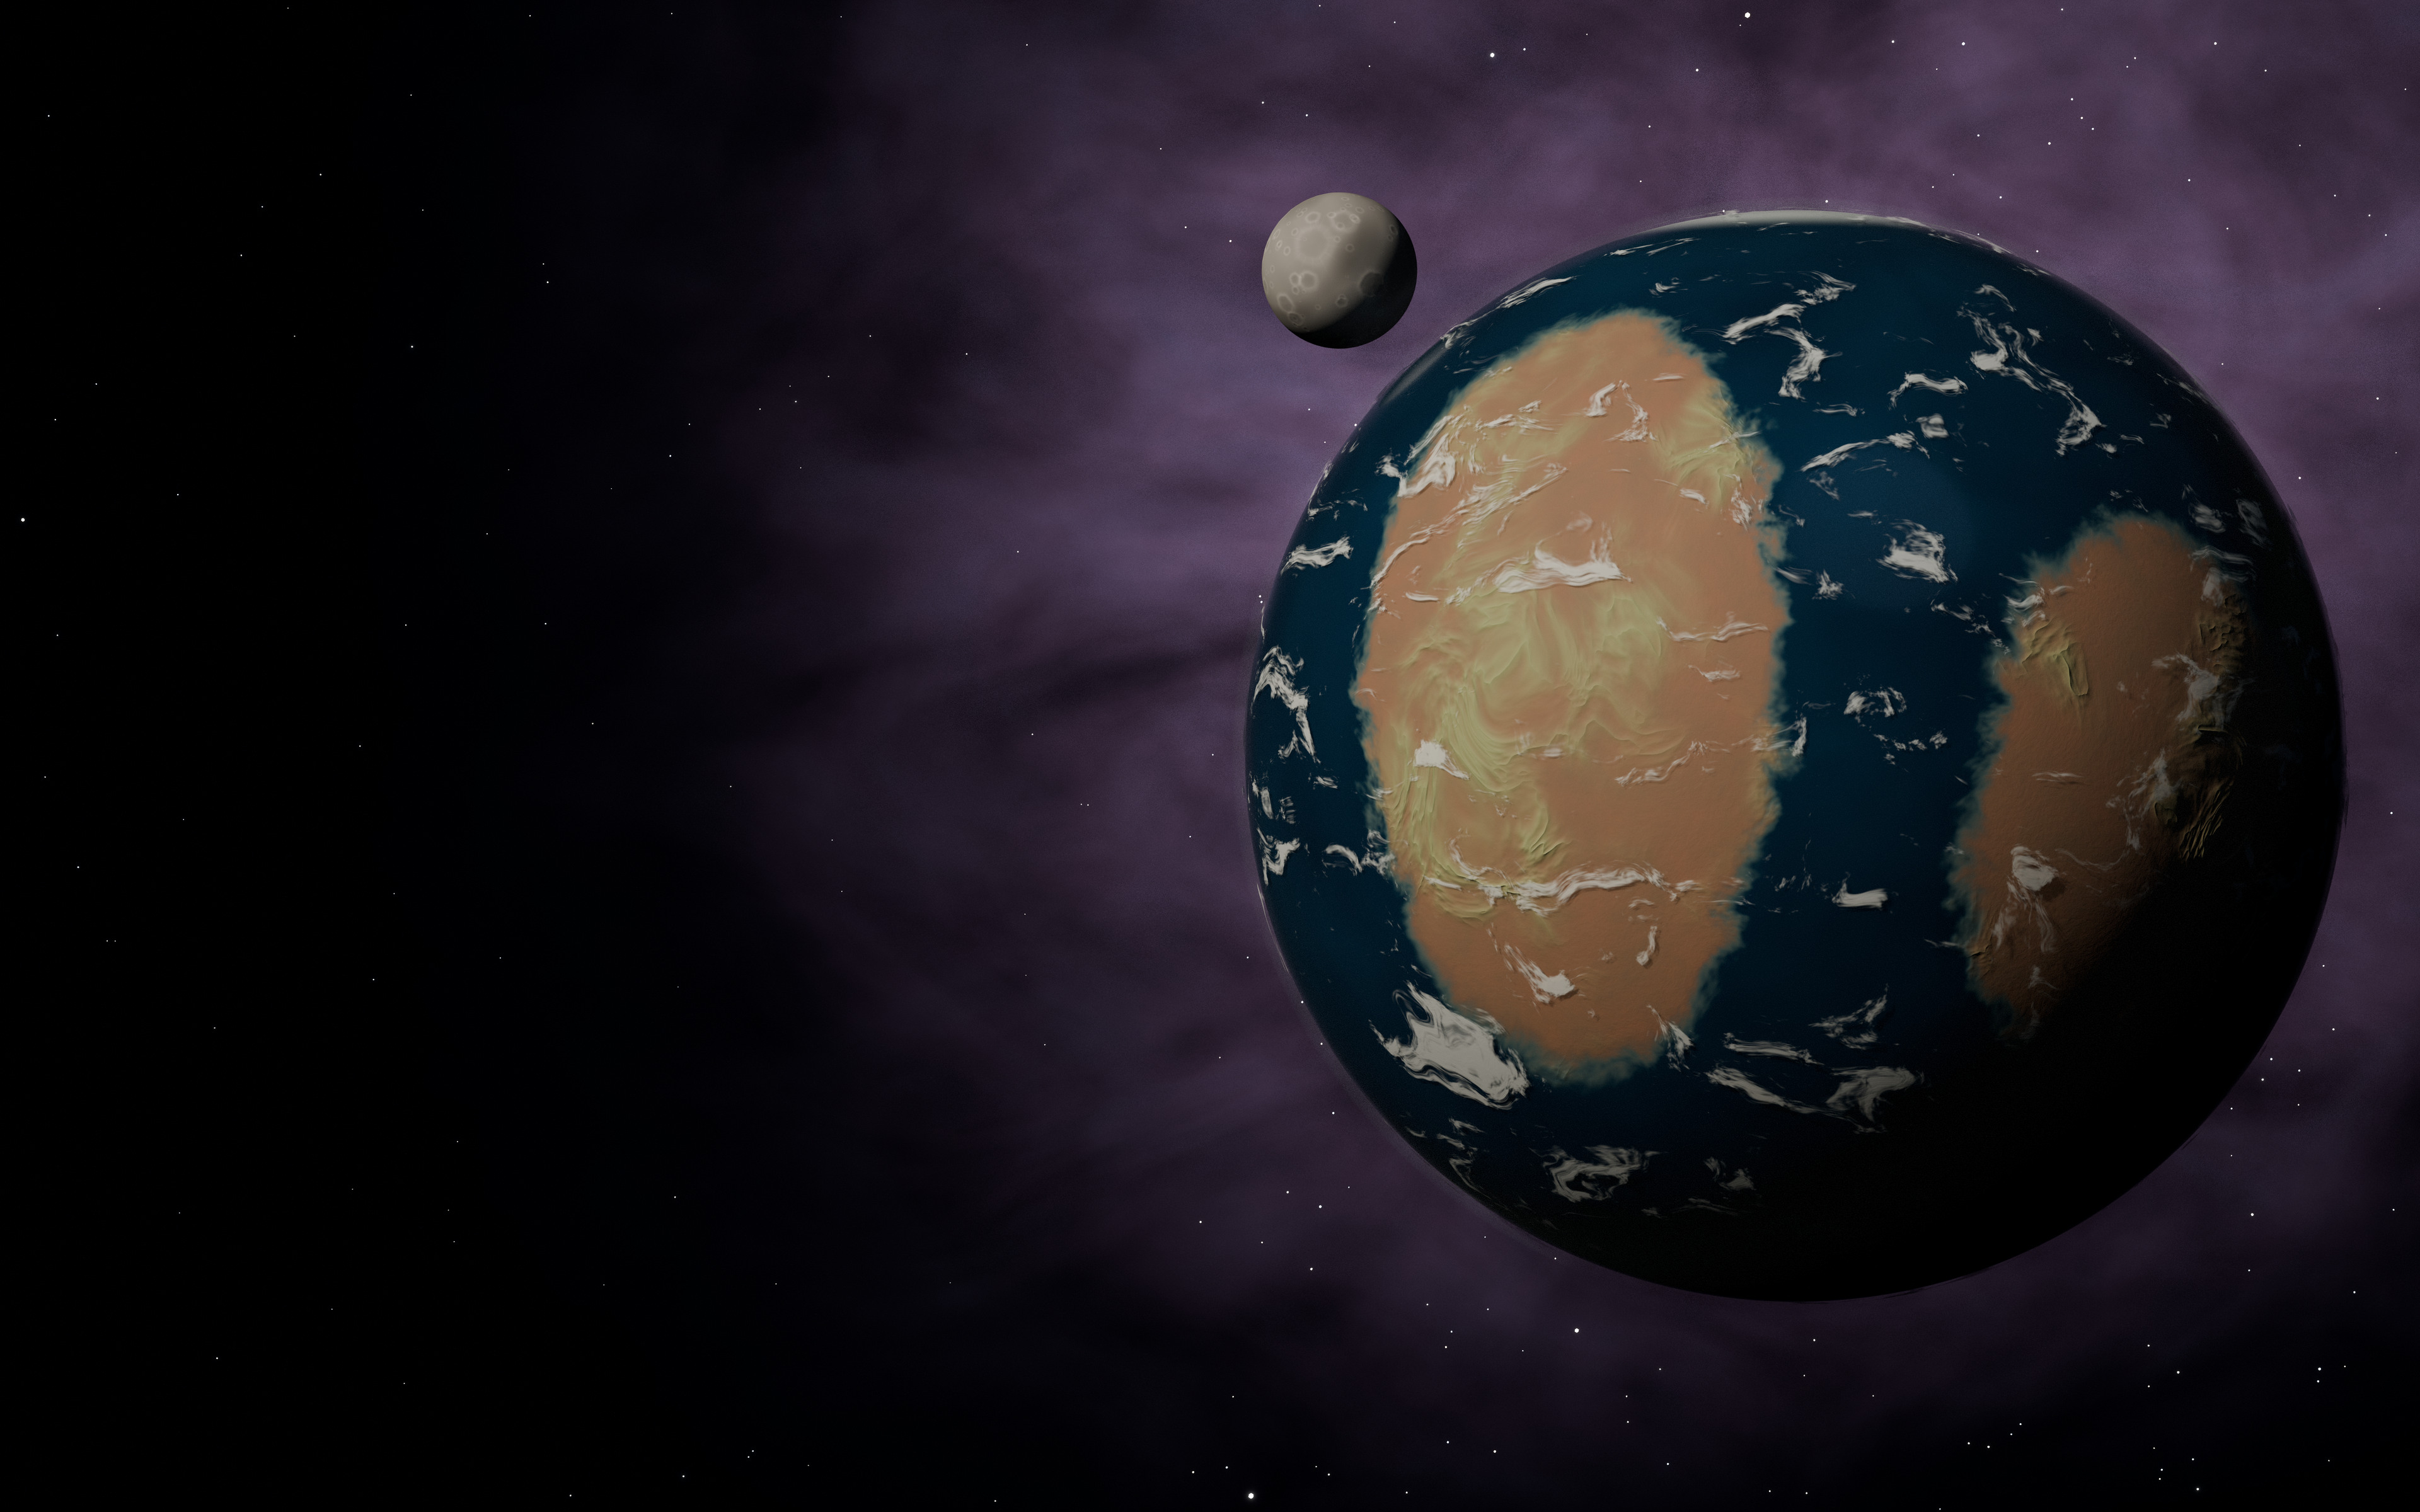
\includegraphics[width=\paperwidth,height=\paperheight]{Risorse/Copertine/M06_Gemina.jpg}};

\node[anchor=north west,inner sep=0,text width=9.2cm] at
 ([xshift=1.05cm,yshift=-1.10cm]current page.north west)
 {\color{Mint}\bfseries\fontsize{23}{27}\selectfont GEMINA};
\node[anchor=north west,inner sep=0,text width=9.2cm] at
 ([xshift=1.07cm,yshift=-2.16cm]current page.north west)
 {\color{white}\fontsize{9.0}{12}\selectfont MODULO M06 · SCIENZE DELLA TERRA};
\draw[Mint,line width=1.4pt] ([xshift=1.05cm,yshift=-2.78cm]current page.north west)--
 ([xshift=2.60cm,yshift=-2.78cm]current page.north west);
\node[anchor=north west,inner sep=0] at
 ([xshift=1.05cm,yshift=-3.35cm]current page.north west)
 {\begin{minipage}{9.2cm}\raggedright\color{white}\bfseries
 \fontsize{30}{36}\selectfont Confrontare\\gruppi e valutare\\ipotesi\end{minipage}};
\node[anchor=north west,inner sep=0] at
 ([xshift=1.07cm,yshift=-7.88cm]current page.north west)
 {\begin{minipage}{9.0cm}\raggedright\color{Lilac}
 \fontsize{12.2}{17}\selectfont Contrasti, test statistici\\e interpretazione dell’evidenza\end{minipage}};
\node[anchor=north west,inner sep=0,text width=9.2cm] at
 ([xshift=1.07cm,yshift=-10.52cm]current page.north west)
 {\color{white}\fontsize{11.5}{15}\selectfont Marzio De Corato};
\node[anchor=north west,inner sep=0,text width=9.2cm] at
 ([xshift=1.07cm,yshift=-11.17cm]current page.north west)
 {\color{Lilac}\fontsize{8.8}{11}\selectfont \href{https://creativecommons.org/licenses/by-nc-sa/4.0/}{\textcopyright{} 2026 · CC BY-NC-SA 4.0}};
\end{tikzpicture}
\end{frame}


\begin{frame}[plain]\hypertarget{slide2}{}
\bookmark[level=0,page=2]{Domanda centrale}
\begin{tikzpicture}[remember picture,overlay]
\node[anchor=north west,inner sep=0] at ([xshift=.95cm,yshift=-.67cm]current page.north west) {\color{Navy}\bfseries\fontsize{23}{27}\selectfont Quando una differenza è evidenza?};
\draw[Classical,line width=1.4pt] ([xshift=.95cm,yshift=-1.73cm]current page.north west)--([xshift=2.5cm,yshift=-1.73cm]current page.north west);
\node[anchor=north west,inner sep=0,fill=GeoTint,rounded corners=2mm,text width=17.7cm,inner sep=3.5mm] at ([xshift=1.0cm,yshift=-2.26cm]current page.north west) {\color{Navy}\fontsize{14.1}{19}\selectfont Come distinguere uno scarto osservato da una conclusione giustificata?};
\node[draw=Rule,line width=.7pt,fill=GeoTint,rounded corners=2.5mm,minimum width=4.8cm,minimum height=2.15cm,text width=4.38cm,align=center,inner sep=3mm] (n0) at ([xshift=4cm,yshift=-6.15cm]current page.north west) {\color{Navy}\bfseries\fontsize{13}{16}\selectfont CONTRASTO\\[2mm]\color{Ink}\normalfont\fontsize{10.5}{14}\selectfont Verso, unità e disegno};
\node[draw=Rule,line width=.7pt,fill=Paper,rounded corners=2.5mm,minimum width=4.8cm,minimum height=2.15cm,text width=4.38cm,align=center,inner sep=3mm] (n1) at ([xshift=10cm,yshift=-6.15cm]current page.north west) {\color{Navy}\bfseries\fontsize{13}{16}\selectfont RIFERIMENTO\\[2mm]\color{Ink}\normalfont\fontsize{10.5}{14}\selectfont Ipotesi nulla e scambiabilità};
\node[draw=Rule,line width=.7pt,fill=GeoTint,rounded corners=2.5mm,minimum width=4.8cm,minimum height=2.15cm,text width=4.38cm,align=center,inner sep=3mm] (n2) at ([xshift=16cm,yshift=-6.15cm]current page.north west) {\color{Navy}\bfseries\fontsize{13}{16}\selectfont EVIDENZA\\[2mm]\color{Ink}\normalfont\fontsize{10.5}{14}\selectfont Effetto, intervallo e test};
\draw[-{Stealth[length=3.0mm]},draw=Classical,line width=1.45pt] ([xshift=6.65cm,yshift=-6.15cm]current page.north west)--([xshift=7.35cm,yshift=-6.15cm]current page.north west);
\draw[-{Stealth[length=3.0mm]},draw=Classical,line width=1.45pt] ([xshift=12.65cm,yshift=-6.15cm]current page.north west)--([xshift=13.35cm,yshift=-6.15cm]current page.north west);
\node[anchor=north west,inner sep=0,text width=17.9cm] at ([xshift=1.05cm,yshift=-8.25cm]current page.north west) {\color{Classical}\bfseries\fontsize{10.4}{13.4}\selectfont IDEA GUIDA};
\node[anchor=north west,inner sep=0,text width=17.85cm] at ([xshift=1.05cm,yshift=-8.71cm]current page.north west) {\color{Ink}\fontsize{11.9}{16.0}\selectfont Un p-value non descrive da solo la grandezza dell’effetto: il confronto deve conservare stima, intervallo e ipotesi.};
\draw[Rule,line width=.35pt] ([xshift=.95cm,yshift=-11.92cm]current page.north west)--([xshift=19.05cm,yshift=-11.92cm]current page.north west);
\node[anchor=north west,inner sep=0] at ([xshift=.95cm,yshift=-12.06cm]current page.north west) {\color{Muted}\fontsize{7.7}{9.3}\selectfont Gemina · Confrontare gruppi e valutare ipotesi};
\node[anchor=north east,inner sep=0] at ([xshift=19.05cm,yshift=-12.06cm]current page.north west) {\color{Muted}\fontsize{7.7}{9.3}\selectfont 2/93};
\end{tikzpicture}
\end{frame}
% SLIDE 003 | Dalla stima al confronto con un’ipotesi
\begin{lrbox}{\PilotLeftBox}%
\begin{minipage}[t]{10.05cm}\raggedright\color{Ink}\fontsize{11.3}{14.8}\selectfont

\PLabel{Il passaggio da Pelago a Gemina}
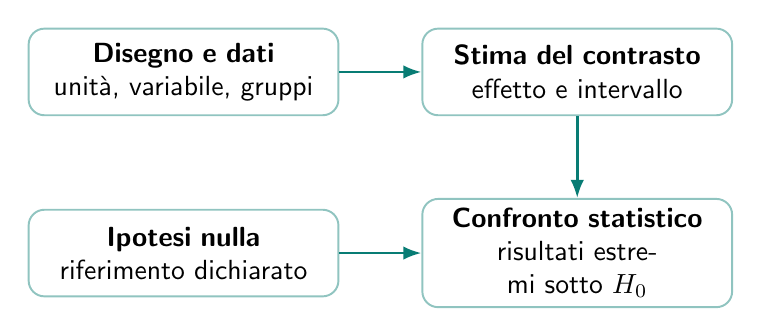
\begin{tikzpicture}[x=1cm,y=1cm]
\node[pFlow,text width=3.7cm] (d) at(2.2,3.4){\textbf{Disegno e dati}\\unità, variabile, gruppi};
\node[pFlow,text width=3.7cm] (s) at(7.2,3.4){\textbf{Stima del contrasto}\\effetto e intervallo};
\node[pFlow,text width=3.7cm] (h) at(2.2,1.1){\textbf{Ipotesi nulla}\\riferimento dichiarato};
\node[pFlow,text width=3.7cm] (t) at(7.2,1.1){\textbf{Confronto statistico}\\risultati estremi sotto $H_0$};
\draw[pEdge](d)--(s);\draw[pEdge](h)--(t);\draw[pEdge](s)--(t);
\end{tikzpicture}
\PBody{Pelago ha introdotto stima e incertezza. Qui aggiungiamo un riferimento nullo, conservando la domanda scientifica e le ipotesi sul campione.}

\end{minipage}% 
\end{lrbox}
\begin{lrbox}{\PilotRightBox}%
\begin{minipage}[t]{7.55cm}\raggedright\color{Ink}\fontsize{11.3}{14.8}\selectfont

\PCode{R · avviare il progetto}{003_avvio.R}
\PSmall{Il file completo \texttt{Lezione\_Gemina.R} raccoglie i frammenti nell’ordine della presentazione.}
\PInfo{Prerequisiti: vettori, tabelle, media, varianza, errore standard e intervalli di confidenza.}

\end{minipage}% 
\end{lrbox}

\begin{frame}[plain]\hypertarget{slide3}{}
\bookmark[level=1,page=3]{Dalla stima al confronto con un’ipotesi}
\begin{tikzpicture}[remember picture,overlay]
\PilotChrome{Dalla stima al confronto con un’ipotesi}{I · DEFINIRE IL CONFRONTO}{3}{Il confronto statistico riguarda un parametro e un disegno espliciti. Stima e incertezza restano parte della conclusione.}
\node[anchor=north west,inner sep=0] at ([xshift=0.96cm,yshift=-2.13cm]current page.north west) {\usebox{\PilotLeftBox}};
\node[anchor=north west,inner sep=0] at ([xshift=11.52cm,yshift=-2.13cm]current page.north west) {\usebox{\PilotRightBox}};

\end{tikzpicture}\end{frame}

% SLIDE 004 | Precisare la domanda prima del calcolo
\begin{lrbox}{\PilotLeftBox}%
\begin{minipage}[t]{10.05cm}\raggedright\color{Ink}\fontsize{11.3}{14.8}\selectfont

\PLabel{Un esempio che attraversa il modulo}
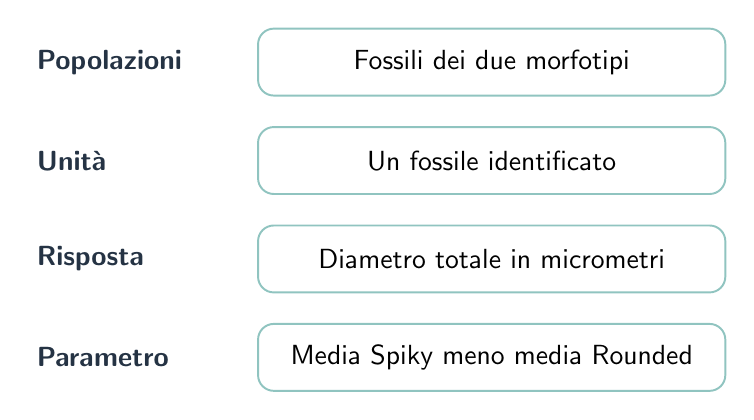
\begin{tikzpicture}[x=1cm,y=1cm]
\foreach \y/\tit/\val in {
4.2/{Popolazioni}/{Fossili dei due morfotipi},
2.95/{Unità}/{Un fossile identificato},
1.7/{Risposta}/{Diametro totale in micrometri},
.45/{Parametro}/{Media Spiky meno media Rounded}}{
\node[pLabel,anchor=west,text width=2.8cm,align=left] at(.25,\y){\textbf{\tit}};
\node[pFlow,text width=5.7cm,minimum height=.85cm] at(6.15,\y){\val};
}
\end{tikzpicture}
\PSmall{Il file del corso contiene 160 fossili sintetici: 80 Rounded e 80 Spiky. Non sono osservazioni raccolte sul terreno.}

\end{minipage}% 
\end{lrbox}
\typeout{FULLBOX:004:L:\the\ht\PilotLeftBox:\the\dp\PilotLeftBox}
\begin{lrbox}{\PilotRightBox}%
\begin{minipage}[t]{7.55cm}\raggedright\color{Ink}\fontsize{11.3}{14.8}\selectfont

\PCode{R · controllare unità e gruppi}{004_domanda.R}
\PSmall{\texttt{table()} conta le osservazioni per gruppo. L’identificativo serve a riconoscere duplicati e abbinamenti.}
\PInfo{L’indipendenza deriva dal disegno. Un identificativo diverso per ogni riga, da solo, non la dimostra.}

\end{minipage}% 
\end{lrbox}
\typeout{FULLBOX:004:R:\the\ht\PilotRightBox:\the\dp\PilotRightBox}
\begin{frame}[plain]\hypertarget{slide4}{}
\bookmark[level=1,page=4]{Precisare la domanda prima del calcolo}
\begin{tikzpicture}[remember picture,overlay]
\PilotChrome{Precisare la domanda prima del calcolo}{I · DEFINIRE IL CONFRONTO}{4}{Una domanda completa specifica popolazioni, unità, variabile, unità di misura e caratteristica da confrontare.}
\node[anchor=north west,inner sep=0] at ([xshift=0.96cm,yshift=-2.13cm]current page.north west) {\usebox{\PilotLeftBox}};
\node[anchor=north west,inner sep=0] at ([xshift=11.52cm,yshift=-2.13cm]current page.north west) {\usebox{\PilotRightBox}};

\end{tikzpicture}\end{frame}

% SLIDE 005 | Il contrasto ha un ordine e un’unità
\begin{lrbox}{\PilotLeftBox}%
\begin{minipage}[t]{10.05cm}\raggedright\color{Ink}\fontsize{11.3}{14.8}\selectfont

\PLabel{Parametro e stima}
\[
\Delta=\mu_B-\mu_A,\qquad
\widehat\Delta=\bar y_B-\bar y_A.
\]
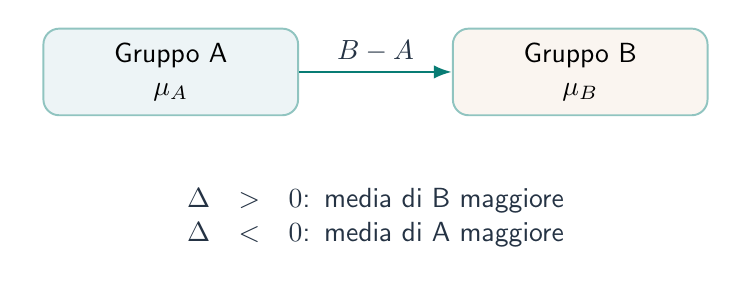
\begin{tikzpicture}[x=1cm,y=1cm]
\node[pFlow,fill=GeoA!8,text width=3.0cm] (a) at(2.0,2.7){Gruppo A\\$\mu_A$};
\node[pFlow,fill=GeoB!8,text width=3.0cm] (b) at(7.2,2.7){Gruppo B\\$\mu_B$};
\draw[pEdge](a.east)--node[above,pLabel]{$B-A$}(b.west);
\node[pLabel,text width=8.6cm] at(4.6,.85){$\Delta>0$: media di B maggiore\\$\Delta<0$: media di A maggiore};
\end{tikzpicture}
\PSmall{$\mu_g$ è la media della popolazione $g$; $\bar y_g$ è la media del campione. Il contrasto mantiene l’unità della variabile.}

\end{minipage}% 
\end{lrbox}
\typeout{FULLBOX:005:L:\the\ht\PilotLeftBox:\the\dp\PilotLeftBox}
\begin{lrbox}{\PilotRightBox}%
\begin{minipage}[t]{7.55cm}\raggedright\color{Ink}\fontsize{11.3}{14.8}\selectfont

\PCode{R · differenza fra due medie}{005_contrasto.R}
\PSmall{\texttt{split()} separa i diametri per morfotipo. Si sottraggono le medie, senza appaiare fossili appartenenti a gruppi indipendenti.}
\PInfo{Nel caso del corso: $A=$ Rounded, $B=$ Spiky; $\Delta$ è espresso in $\mu$m.}

\end{minipage}% 
\end{lrbox}
\typeout{FULLBOX:005:R:\the\ht\PilotRightBox:\the\dp\PilotRightBox}
\begin{frame}[plain]\hypertarget{slide5}{}
\bookmark[level=1,page=5]{Il contrasto ha un ordine e un’unità}
\begin{tikzpicture}[remember picture,overlay]
\PilotChrome{Il contrasto ha un ordine e un’unità}{I · DEFINIRE IL CONFRONTO}{5}{Il segno descrive una direzione convenzionale. Va dichiarato prima di leggere stima, intervallo e risultato del test.}
\node[anchor=north west,inner sep=0] at ([xshift=0.96cm,yshift=-2.13cm]current page.north west) {\usebox{\PilotLeftBox}};
\node[anchor=north west,inner sep=0] at ([xshift=11.52cm,yshift=-2.13cm]current page.north west) {\usebox{\PilotRightBox}};

\end{tikzpicture}\end{frame}

% SLIDE 006 | Cambiare segno o unità cambia la lettura
\begin{lrbox}{\PilotLeftBox}%
\begin{minipage}[t]{10.05cm}\raggedright\color{Ink}\fontsize{11.3}{14.8}\selectfont

\PLabel{La stessa differenza, due rappresentazioni}
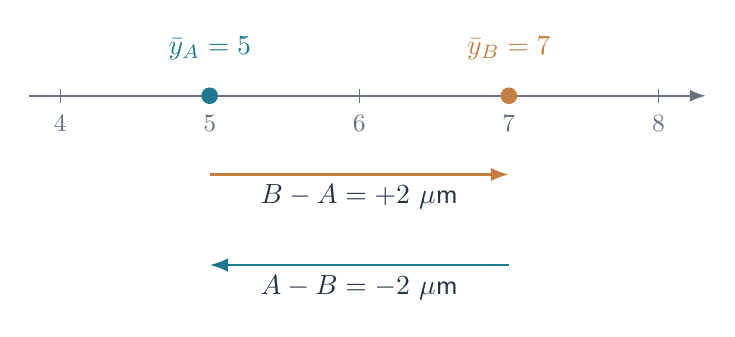
\begin{tikzpicture}[x=1cm,y=1cm]
\draw[pAxis](.6,2.65)--(9.2,2.65);
\foreach \x/\v in {1.0/4,2.9/5,4.8/6,6.7/7,8.6/8}{
\draw[Muted](\x,2.56)--(\x,2.74);
\node[pNote] at(\x,2.3){$\v$};}
\fill[GeoA](2.9,2.65) circle(3pt);
\fill[GeoB](6.7,2.65) circle(3pt);
\node[pLabel,text=GeoA] at(2.9,3.25){$\bar y_A=5$};
\node[pLabel,text=GeoB] at(6.7,3.25){$\bar y_B=7$};
\draw[pEdge,GeoB](2.9,1.65)--node[below,pLabel]{$B-A=+2\ \mu$m}(6.7,1.65);
\draw[pEdge,GeoA](6.7,.5)--node[below,pLabel]{$A-B=-2\ \mu$m}(2.9,.5);
\end{tikzpicture}
\PSmall{Convertendo da $\mu$m a mm, $2\ \mu$m diventano $0{,}002$ mm. Anche errore standard e limiti dell’intervallo vanno convertiti.}

\end{minipage}% 
\end{lrbox}
\typeout{FULLBOX:006:L:\the\ht\PilotLeftBox:\the\dp\PilotLeftBox}
\begin{lrbox}{\PilotRightBox}%
\begin{minipage}[t]{7.55cm}\raggedright\color{Ink}\fontsize{11.3}{14.8}\selectfont

\PCode{R · mantenere coerente il contrasto}{006_segno.R}
\PSmall{Il test bilaterale restituisce lo stesso $p$ invertendo i gruppi. Il segno della statistica cambia e l’intervallo si riflette rispetto a zero.}
\PInfo{Se $IC_{B-A}=[L,U]$, allora $IC_{A-B}=[-U,-L]$.}

\end{minipage}% 
\end{lrbox}
\typeout{FULLBOX:006:R:\the\ht\PilotRightBox:\the\dp\PilotRightBox}
\begin{frame}[plain]\hypertarget{slide6}{}
\bookmark[level=1,page=6]{Cambiare segno o unità cambia la lettura}
\begin{tikzpicture}[remember picture,overlay]
\PilotChrome{Cambiare segno o unità cambia la lettura}{I · DEFINIRE IL CONFRONTO}{6}{La direzione della sottrazione e l’unità devono restare coerenti in codice, grafici e relazione.}
\node[anchor=north west,inner sep=0] at ([xshift=0.96cm,yshift=-2.13cm]current page.north west) {\usebox{\PilotLeftBox}};
\node[anchor=north west,inner sep=0] at ([xshift=11.52cm,yshift=-2.13cm]current page.north west) {\usebox{\PilotRightBox}};

\end{tikzpicture}\end{frame}

% SLIDE 007 | Il disegno stabilisce le unità indipendenti
\begin{lrbox}{\PilotLeftBox}%
\begin{minipage}[t]{10.05cm}\raggedright\color{Ink}\fontsize{11.3}{14.8}\selectfont

\PLabel{Tre strutture da riconoscere}
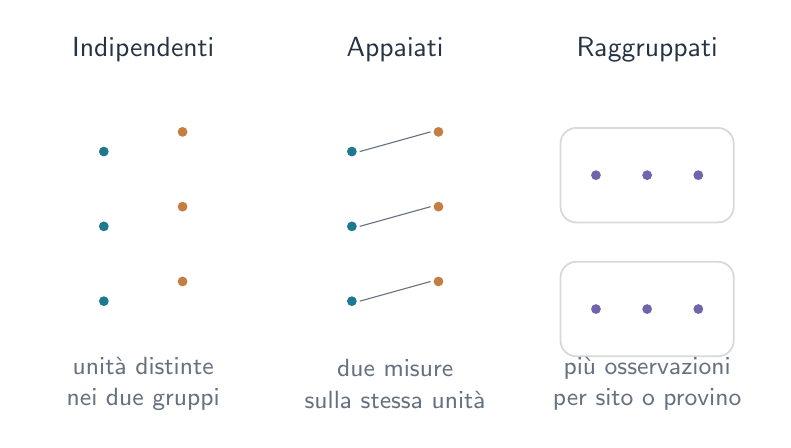
\begin{tikzpicture}[x=1cm,y=1cm]
\node[pLabel] at(1.6,4.5){Indipendenti};
\node[pLabel] at(4.8,4.5){Appaiati};
\node[pLabel] at(8.0,4.5){Raggruppati};
\foreach \y in {1.3,2.25,3.2}{
\node[pDotA] at(1.1,\y){};
\node[pDotB] at(2.1,\y+.25){};
\node[pDotA] at(4.25,\y){};
\node[pDotB] at(5.35,\y+.25){};
\draw[Muted](4.35,\y)--(5.25,\y+.25);
}
\foreach \y in {1.2,2.9}{
\draw[pGroup](6.9,\y-.6) rectangle(9.1,\y+.6);
\foreach \x in {7.35,8,8.65}\node[pDotC] at(\x,\y){};
}
\node[pNote,text width=2.7cm] at(1.6,.25){unità distinte\\nei due gruppi};
\node[pNote,text width=2.7cm] at(4.8,.25){due misure\\sulla stessa unità};
\node[pNote,text width=2.7cm] at(8,.25){più osservazioni\\per sito o provino};
\end{tikzpicture}
\PSmall{Le linee indicano legami del disegno. I gruppi di osservazioni dello stesso sito possono condividere condizioni ambientali.}

\end{minipage}% 
\end{lrbox}
\typeout{FULLBOX:007:L:\the\ht\PilotLeftBox:\the\dp\PilotLeftBox}
\begin{lrbox}{\PilotRightBox}%
\begin{minipage}[t]{7.55cm}\raggedright\color{Ink}\fontsize{11.3}{14.8}\selectfont

\PCode{R · contare righe e coppie}{007_disegno.R}
\PSmall{Il numero di righe è 8; le unità con una misura prima e una dopo sono 4. Nel test appaiato $n$ conta coppie complete.}
\PInfo{Un test per campioni indipendenti richiede una giustificazione dell’indipendenza fra le unità utilizzate.}

\end{minipage}% 
\end{lrbox}
\typeout{FULLBOX:007:R:\the\ht\PilotRightBox:\the\dp\PilotRightBox}
\begin{frame}[plain]\hypertarget{slide7}{}
\bookmark[level=1,page=7]{Il disegno stabilisce le unità indipendenti}
\begin{tikzpicture}[remember picture,overlay]
\PilotChrome{Il disegno stabilisce le unità indipendenti}{I · DEFINIRE IL CONFRONTO}{7}{L’unità di analisi dipende dal prelievo e dagli abbinamenti. Contare le righe non basta a determinare la numerosità informativa.}
\node[anchor=north west,inner sep=0] at ([xshift=0.96cm,yshift=-2.13cm]current page.north west) {\usebox{\PilotLeftBox}};
\node[anchor=north west,inner sep=0] at ([xshift=11.52cm,yshift=-2.13cm]current page.north west) {\usebox{\PilotRightBox}};

\end{tikzpicture}\end{frame}

% SLIDE 008 | Osservare tutti i valori dei due gruppi
\begin{lrbox}{\PilotLeftBox}%
\begin{minipage}[t]{10.05cm}\raggedright\color{Ink}\fontsize{11.3}{14.8}\selectfont
\PLabel{Diametri sintetici del corso}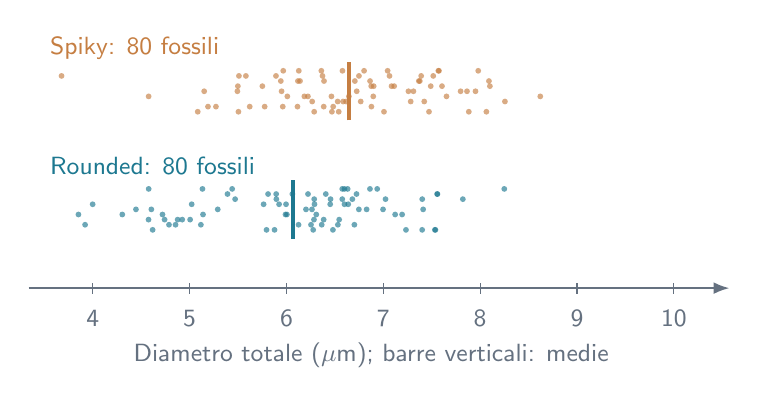
\begin{tikzpicture}[x=1cm,y=1cm]
\draw[pAxis](.45,.5)--(9.35,.5);
\draw[Muted](1.265,.43)--(1.265,.57);
\node[pNote] at(1.265,.12){4};
\draw[Muted](2.495,.43)--(2.495,.57);
\node[pNote] at(2.495,.12){5};
\draw[Muted](3.725,.43)--(3.725,.57);
\node[pNote] at(3.725,.12){6};
\draw[Muted](4.955,.43)--(4.955,.57);
\node[pNote] at(4.955,.12){7};
\draw[Muted](6.185,.43)--(6.185,.57);
\node[pNote] at(6.185,.12){8};
\draw[Muted](7.415,.43)--(7.415,.57);
\node[pNote] at(7.415,.12){9};
\draw[Muted](8.645,.43)--(8.645,.57);
\node[pNote] at(8.645,.12){10};
\node[pNote,text=GeoA,anchor=west] at(.6,2.05){Rounded: 80 fossili};
\fill[GeoA,opacity=.65](5.2430,1.2400) circle(1.05pt);
\fill[GeoA,opacity=.65](3.4916,1.6950) circle(1.05pt);
\fill[GeoA,opacity=.65](4.5096,1.5650) circle(1.05pt);
\fill[GeoA,opacity=.65](1.6404,1.4350) circle(1.05pt);
\fill[GeoA,opacity=.65](4.1727,1.3050) circle(1.05pt);
\fill[GeoA,opacity=.65](4.8777,1.7600) circle(1.05pt);
\fill[GeoA,opacity=.65](4.0774,1.6300) circle(1.05pt);
\fill[GeoA,opacity=.65](4.6448,1.5000) circle(1.05pt);
\fill[GeoA,opacity=.65](2.3431,1.3700) circle(1.05pt);
\fill[GeoA,opacity=.65](4.0646,1.2400) circle(1.05pt);
\fill[GeoA,opacity=.65](3.5946,1.6950) circle(1.05pt);
\fill[GeoA,opacity=.65](3.7198,1.5650) circle(1.05pt);
\fill[GeoA,opacity=.65](2.1506,1.4350) circle(1.05pt);
\fill[GeoA,opacity=.65](1.1678,1.3050) circle(1.05pt);
\fill[GeoA,opacity=.65](4.7856,1.7600) circle(1.05pt);
\fill[GeoA,opacity=.65](5.4495,1.6300) circle(1.05pt);
\fill[GeoA,opacity=.65](2.0094,1.5000) circle(1.05pt);
\fill[GeoA,opacity=.65](4.1976,1.3700) circle(1.05pt);
\fill[GeoA,opacity=.65](5.4485,1.2400) circle(1.05pt);
\fill[GeoA,opacity=.65](3.8001,1.6950) circle(1.05pt);
\fill[GeoA,opacity=.65](4.2805,1.5650) circle(1.05pt);
\fill[GeoA,opacity=.65](4.1037,1.4350) circle(1.05pt);
\fill[GeoA,opacity=.65](2.3166,1.3050) circle(1.05pt);
\fill[GeoA,opacity=.65](2.6584,1.7600) circle(1.05pt);
\fill[GeoA,opacity=.65](4.4339,1.6300) circle(1.05pt);
\fill[GeoA,opacity=.65](5.4609,1.5000) circle(1.05pt);
\fill[GeoA,opacity=.65](1.9735,1.3700) circle(1.05pt);
\fill[GeoA,opacity=.65](3.5737,1.2400) circle(1.05pt);
\fill[GeoA,opacity=.65](5.6422,1.6950) circle(1.05pt);
\fill[GeoA,opacity=.65](2.5214,1.5650) circle(1.05pt);
\fill[GeoA,opacity=.65](3.7306,1.4350) circle(1.05pt);
\fill[GeoA,opacity=.65](2.2334,1.3050) circle(1.05pt);
\fill[GeoA,opacity=.65](4.4618,1.7600) circle(1.05pt);
\fill[GeoA,opacity=.65](5.9652,1.6300) circle(1.05pt);
\fill[GeoA,opacity=.65](2.8525,1.5000) circle(1.05pt);
\fill[GeoA,opacity=.65](2.5015,1.3700) circle(1.05pt);
\fill[GeoA,opacity=.65](2.0255,1.2400) circle(1.05pt);
\fill[GeoA,opacity=.65](3.9989,1.6950) circle(1.05pt);
\fill[GeoA,opacity=.65](3.6316,1.5650) circle(1.05pt);
\fill[GeoA,opacity=.65](1.0833,1.4350) circle(1.05pt);
\fill[GeoA,opacity=.65](4.5878,1.3050) circle(1.05pt);
\fill[GeoA,opacity=.65](3.0355,1.7600) circle(1.05pt);
\fill[GeoA,opacity=.65](4.5622,1.6300) circle(1.05pt);
\fill[GeoA,opacity=.65](4.7431,1.5000) circle(1.05pt);
\fill[GeoA,opacity=.65](2.4011,1.3700) circle(1.05pt);
\fill[GeoA,opacity=.65](5.6103,1.2400) circle(1.05pt);
\fill[GeoA,opacity=.65](4.6149,1.6950) circle(1.05pt);
\fill[GeoA,opacity=.65](3.4349,1.5650) circle(1.05pt);
\fill[GeoA,opacity=.65](2.6655,1.4350) circle(1.05pt);
\fill[GeoA,opacity=.65](3.8788,1.3050) circle(1.05pt);
\fill[GeoA,opacity=.65](1.9751,1.7600) circle(1.05pt);
\fill[GeoA,opacity=.65](4.2849,1.6300) circle(1.05pt);
\fill[GeoA,opacity=.65](1.8136,1.5000) circle(1.05pt);
\fill[GeoA,opacity=.65](2.1775,1.3700) circle(1.05pt);
\fill[GeoA,opacity=.65](4.3150,1.2400) circle(1.05pt);
\fill[GeoA,opacity=.65](5.6390,1.6950) circle(1.05pt);
\fill[GeoA,opacity=.65](4.4620,1.5650) circle(1.05pt);
\fill[GeoA,opacity=.65](5.1055,1.4350) circle(1.05pt);
\fill[GeoA,opacity=.65](4.0369,1.3050) circle(1.05pt);
\fill[GeoA,opacity=.65](4.5021,1.7600) circle(1.05pt);
\fill[GeoA,opacity=.65](4.9831,1.6300) circle(1.05pt);
\fill[GeoA,opacity=.65](4.9517,1.5000) circle(1.05pt);
\fill[GeoA,opacity=.65](4.3944,1.3700) circle(1.05pt);
\fill[GeoA,opacity=.65](3.4719,1.2400) circle(1.05pt);
\fill[GeoA,opacity=.65](2.9763,1.6950) circle(1.05pt);
\fill[GeoA,opacity=.65](4.0809,1.5650) circle(1.05pt);
\fill[GeoA,opacity=.65](5.1939,1.4350) circle(1.05pt);
\fill[GeoA,opacity=.65](4.3780,1.3050) circle(1.05pt);
\fill[GeoA,opacity=.65](6.4916,1.7600) circle(1.05pt);
\fill[GeoA,opacity=.65](3.0732,1.6300) circle(1.05pt);
\fill[GeoA,opacity=.65](4.0491,1.5000) circle(1.05pt);
\fill[GeoA,opacity=.65](4.0746,1.3700) circle(1.05pt);
\fill[GeoA,opacity=.65](5.6168,1.2400) circle(1.05pt);
\fill[GeoA,opacity=.65](4.2247,1.6950) circle(1.05pt);
\fill[GeoA,opacity=.65](1.2638,1.5650) circle(1.05pt);
\fill[GeoA,opacity=.65](3.7123,1.4350) circle(1.05pt);
\fill[GeoA,opacity=.65](2.6382,1.3050) circle(1.05pt);
\fill[GeoA,opacity=.65](4.4338,1.7600) circle(1.05pt);
\fill[GeoA,opacity=.65](3.5967,1.6300) circle(1.05pt);
\fill[GeoA,opacity=.65](3.9728,1.5000) circle(1.05pt);
\draw[GeoA,line width=1.4pt](3.8033,1.13)--(3.8033,1.87);
\node[pNote,text=GeoB,anchor=west] at(.6,3.55){Spiky: 80 fossili};
\fill[GeoB,opacity=.65](5.5354,2.7400) circle(1.05pt);
\fill[GeoB,opacity=.65](5.0337,3.1950) circle(1.05pt);
\fill[GeoB,opacity=.65](3.1080,3.0650) circle(1.05pt);
\fill[GeoB,opacity=.65](4.5180,2.9350) circle(1.05pt);
\fill[GeoB,opacity=.65](3.8652,2.8050) circle(1.05pt);
\fill[GeoB,opacity=.65](3.6844,3.2600) circle(1.05pt);
\fill[GeoB,opacity=.65](4.7867,3.1300) circle(1.05pt);
\fill[GeoB,opacity=.65](3.1021,3.0000) circle(1.05pt);
\fill[GeoB,opacity=.65](6.4997,2.8700) circle(1.05pt);
\fill[GeoB,opacity=.65](2.5984,2.7400) circle(1.05pt);
\fill[GeoB,opacity=.65](0.8688,3.1950) circle(1.05pt);
\fill[GeoB,opacity=.65](5.0930,3.0650) circle(1.05pt);
\fill[GeoB,opacity=.65](3.7365,2.9350) circle(1.05pt);
\fill[GeoB,opacity=.65](3.2584,2.8050) circle(1.05pt);
\fill[GeoB,opacity=.65](6.1605,3.2600) circle(1.05pt);
\fill[GeoB,opacity=.65](3.8974,3.1300) circle(1.05pt);
\fill[GeoB,opacity=.65](5.9365,3.0000) circle(1.05pt);
\fill[GeoB,opacity=.65](5.4750,2.8700) circle(1.05pt);
\fill[GeoB,opacity=.65](4.3023,2.7400) circle(1.05pt);
\fill[GeoB,opacity=.65](3.5920,3.1950) circle(1.05pt);
\fill[GeoB,opacity=.65](3.4193,3.0650) circle(1.05pt);
\fill[GeoB,opacity=.65](5.7576,2.9350) circle(1.05pt);
\fill[GeoB,opacity=.65](3.4481,2.8050) circle(1.05pt);
\fill[GeoB,opacity=.65](5.6541,3.2600) circle(1.05pt);
\fill[GeoB,opacity=.65](4.2022,3.1300) circle(1.05pt);
\fill[GeoB,opacity=.65](2.6801,3.0000) circle(1.05pt);
\fill[GeoB,opacity=.65](4.6679,2.8700) circle(1.05pt);
\fill[GeoB,opacity=.65](3.1152,2.7400) circle(1.05pt);
\fill[GeoB,opacity=.65](3.2099,3.1950) circle(1.05pt);
\fill[GeoB,opacity=.65](5.0595,3.0650) circle(1.05pt);
\fill[GeoB,opacity=.65](4.2961,2.9350) circle(1.05pt);
\fill[GeoB,opacity=.65](2.7285,2.8050) circle(1.05pt);
\fill[GeoB,opacity=.65](5.0100,3.2600) circle(1.05pt);
\fill[GeoB,opacity=.65](3.8708,3.1300) circle(1.05pt);
\fill[GeoB,opacity=.65](3.6631,3.0000) circle(1.05pt);
\fill[GeoB,opacity=.65](4.3755,2.8700) circle(1.05pt);
\fill[GeoB,opacity=.65](6.0410,2.7400) circle(1.05pt);
\fill[GeoB,opacity=.65](5.4360,3.1950) circle(1.05pt);
\fill[GeoB,opacity=.65](5.5573,3.0650) circle(1.05pt);
\fill[GeoB,opacity=.65](6.9488,2.9350) circle(1.05pt);
\fill[GeoB,opacity=.65](2.8295,2.8050) circle(1.05pt);
\fill[GeoB,opacity=.65](4.1683,3.2600) circle(1.05pt);
\fill[GeoB,opacity=.65](5.4187,3.1300) circle(1.05pt);
\fill[GeoB,opacity=.65](6.0178,3.0000) circle(1.05pt);
\fill[GeoB,opacity=.65](4.4445,2.8700) circle(1.05pt);
\fill[GeoB,opacity=.65](4.3890,2.7400) circle(1.05pt);
\fill[GeoB,opacity=.65](4.1829,3.1950) circle(1.05pt);
\fill[GeoB,opacity=.65](4.8326,3.0650) circle(1.05pt);
\fill[GeoB,opacity=.65](3.9977,2.9350) circle(1.05pt);
\fill[GeoB,opacity=.65](3.6784,2.8050) circle(1.05pt);
\fill[GeoB,opacity=.65](3.8818,3.2600) circle(1.05pt);
\fill[GeoB,opacity=.65](4.5937,3.1300) circle(1.05pt);
\fill[GeoB,opacity=.65](6.1260,3.0000) circle(1.05pt);
\fill[GeoB,opacity=.65](4.4827,2.8700) circle(1.05pt);
\fill[GeoB,opacity=.65](4.9637,2.7400) circle(1.05pt);
\fill[GeoB,opacity=.65](4.6457,3.1950) circle(1.05pt);
\fill[GeoB,opacity=.65](6.3086,3.0650) circle(1.05pt);
\fill[GeoB,opacity=.65](1.9746,2.9350) circle(1.05pt);
\fill[GeoB,opacity=.65](4.3183,2.8050) circle(1.05pt);
\fill[GeoB,opacity=.65](5.6621,3.2600) circle(1.05pt);
\fill[GeoB,opacity=.65](6.2966,3.1300) circle(1.05pt);
\fill[GeoB,opacity=.65](5.2742,3.0000) circle(1.05pt);
\fill[GeoB,opacity=.65](4.0517,2.8700) circle(1.05pt);
\fill[GeoB,opacity=.65](6.2642,2.7400) circle(1.05pt);
\fill[GeoB,opacity=.65](3.1214,3.1950) circle(1.05pt);
\fill[GeoB,opacity=.65](5.7005,3.0650) circle(1.05pt);
\fill[GeoB,opacity=.65](4.8276,2.9350) circle(1.05pt);
\fill[GeoB,opacity=.65](4.1983,2.8050) circle(1.05pt);
\fill[GeoB,opacity=.65](4.7110,3.2600) circle(1.05pt);
\fill[GeoB,opacity=.65](5.4060,3.1300) circle(1.05pt);
\fill[GeoB,opacity=.65](5.3377,3.0000) circle(1.05pt);
\fill[GeoB,opacity=.65](5.3027,2.8700) circle(1.05pt);
\fill[GeoB,opacity=.65](4.0771,2.7400) circle(1.05pt);
\fill[GeoB,opacity=.65](5.5894,3.1950) circle(1.05pt);
\fill[GeoB,opacity=.65](4.8014,3.0650) circle(1.05pt);
\fill[GeoB,opacity=.65](3.9525,2.9350) circle(1.05pt);
\fill[GeoB,opacity=.65](4.8038,2.8050) circle(1.05pt);
\fill[GeoB,opacity=.65](4.4362,3.2600) circle(1.05pt);
\fill[GeoB,opacity=.65](3.6535,3.1300) circle(1.05pt);
\fill[GeoB,opacity=.65](4.6171,3.0000) circle(1.05pt);
\draw[GeoB,line width=1.4pt](4.5192,2.63)--(4.5192,3.37);
\node[pNote] at(4.8,-.35){Diametro totale ($\mu$m); barre verticali: medie};
\end{tikzpicture}
\PSmall{Ogni punto rappresenta un fossile. Lo spostamento verticale rende visibili le sovrapposizioni; l’altezza dei punti non è una seconda variabile.}

\end{minipage}% 
\end{lrbox}
\typeout{FULLBOX:008:L:\the\ht\PilotLeftBox:\the\dp\PilotLeftBox}
\begin{lrbox}{\PilotRightBox}%
\begin{minipage}[t]{7.55cm}\raggedright\color{Ink}\fontsize{11.3}{14.8}\selectfont

\PCode{R · distribuzioni e medie}{008_punti.R}
\PSmall{Il codice impila i punti sovrapposti. Si osservano dispersione, asimmetria e valori estremi.}
\PInfo{I valori individuali permettono di valutare quanto la media rappresenti il gruppo.}

\end{minipage}% 
\end{lrbox}
\typeout{FULLBOX:008:R:\the\ht\PilotRightBox:\the\dp\PilotRightBox}
\begin{frame}[plain]\hypertarget{slide8}{}
\bookmark[level=1,page=8]{Osservare tutti i valori dei due gruppi}
\begin{tikzpicture}[remember picture,overlay]
\PilotChrome{Osservare tutti i valori dei due gruppi}{I · DEFINIRE IL CONFRONTO}{8}{Il grafico dei dati precede l’interpretazione del test e permette di riconoscere aspetti che una media da sola non descrive.}
\node[anchor=north west,inner sep=0] at ([xshift=0.96cm,yshift=-2.13cm]current page.north west) {\usebox{\PilotLeftBox}};
\node[anchor=north west,inner sep=0] at ([xshift=11.52cm,yshift=-2.13cm]current page.north west) {\usebox{\PilotRightBox}};

\end{tikzpicture}\end{frame}

% SLIDE 009 | Medie diverse e individui sovrapposti
\begin{lrbox}{\PilotLeftBox}%
\begin{minipage}[t]{10.05cm}\raggedright\color{Ink}\fontsize{11.3}{14.8}\selectfont

\PLabel{Due quantità rispondono a domande diverse}
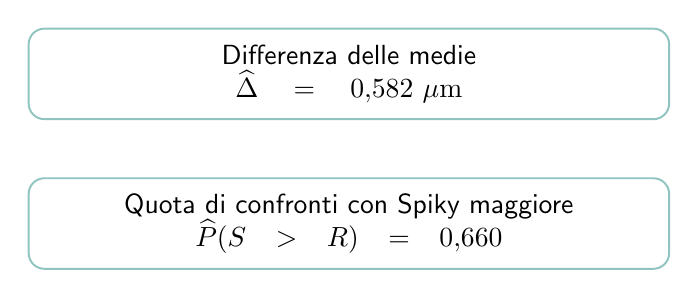
\begin{tikzpicture}[x=1cm,y=1cm]
\node[pFlow,text width=7.9cm,minimum height=1.15cm] at(4.7,3.7)
{Differenza delle medie\\$\widehat\Delta=0{,}582\ \mu\mathrm m$};
\node[pFlow,text width=7.9cm,minimum height=1.15cm] at(4.7,1.8)
{Quota di confronti con Spiky maggiore\\$\widehat P(S>R)=0{,}660$};
\end{tikzpicture}
\PBody{Una differenza media positiva può accompagnarsi a molti individui Rounded più grandi di alcuni Spiky.}
\PSmall{Qui non ci sono pareggi. Per la probabilità di superiorità con pareggi assegneremo metà contributo a ciascuna uguaglianza.}

\end{minipage}% 
\end{lrbox}
\typeout{FULLBOX:009:L:\the\ht\PilotLeftBox:\the\dp\PilotLeftBox}
\begin{lrbox}{\PilotRightBox}%
\begin{minipage}[t]{7.55cm}\raggedright\color{Ink}\fontsize{11.3}{14.8}\selectfont

\PCode{R · medie e confronti individuali}{009_medie_individui.R}
\PSmall{\texttt{outer()} confronta ciascuno degli 80 Spiky con ciascuno degli 80 Rounded: $80\times80=6400$ confronti.}
\PInfo{I 6400 confronti condividono gli stessi 160 individui. Non costituiscono 6400 osservazioni indipendenti.}

\end{minipage}% 
\end{lrbox}
\typeout{FULLBOX:009:R:\the\ht\PilotRightBox:\the\dp\PilotRightBox}
\begin{frame}[plain]\hypertarget{slide9}{}
\bookmark[level=1,page=9]{Medie diverse e individui sovrapposti}
\begin{tikzpicture}[remember picture,overlay]
\PilotChrome{Medie diverse e individui sovrapposti}{I · DEFINIRE IL CONFRONTO}{9}{Una differenza fra medie non separa necessariamente gli individui. La probabilità di superiorità è un altro parametro.}
\node[anchor=north west,inner sep=0] at ([xshift=0.96cm,yshift=-2.13cm]current page.north west) {\usebox{\PilotLeftBox}};
\node[anchor=north west,inner sep=0] at ([xshift=11.52cm,yshift=-2.13cm]current page.north west) {\usebox{\PilotRightBox}};

\end{tikzpicture}\end{frame}

% SLIDE 010 | Accompagnare l’effetto con l’incertezza
\begin{lrbox}{\PilotLeftBox}%
\begin{minipage}[t]{10.05cm}\raggedright\color{Ink}\fontsize{11.3}{14.8}\selectfont
\PLabel{Intervallo di Welch per la differenza}
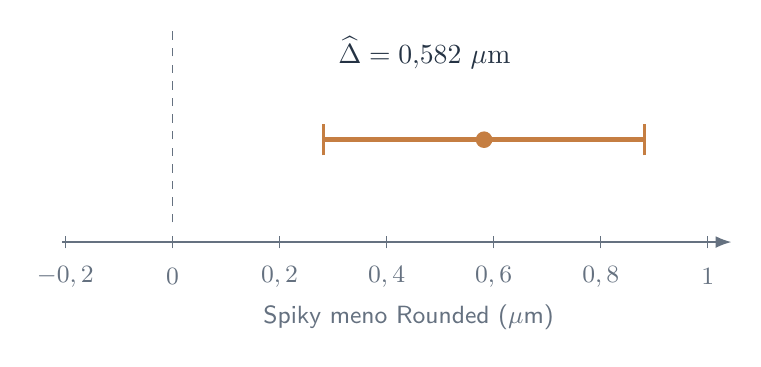
\begin{tikzpicture}[x=1cm,y=1cm]
\draw[pAxis](.6,.8)--(9.1,.8);
\foreach \v/\lab in {-.2/{-0,2},0/0,.2/{0,2},.4/{0,4},.6/{0,6},.8/{0,8},1/1}{
\pgfmathsetmacro{\xx}{2+6.8*\v}
\draw[Muted](\xx,.72)--(\xx,.88);
\node[pNote] at(\xx,.36){$\lab$};}
\draw[Muted,dashed](2,1.05)--(2,3.5);
\draw[GeoB,line width=2pt](3.9173,2.1)--(7.9983,2.1);
\foreach \xx in {3.9173,7.9983}
\draw[GeoB,line width=1pt](\xx,1.9)--(\xx,2.3);
\fill[GeoB](5.9578,2.1) circle(3pt);
\node[pLabel] at(5.2,3.2){$\widehat\Delta=0{,}582\ \mu\mathrm m$};
\node[pNote] at(5.0,-.15){Spiky meno Rounded ($\mu$m)};
\end{tikzpicture}

\PSmall{Nel caso dei fossili: $IC_{95\%}=[0{,}282;0{,}882]\ \mu$m e $SE=0{,}152\ \mu$m. La derivazione di Welch inizia alla slide 37.}

\end{minipage}% 
\end{lrbox}
\typeout{FULLBOX:010:L:\the\ht\PilotLeftBox:\the\dp\PilotLeftBox}
\begin{lrbox}{\PilotRightBox}%
\begin{minipage}[t]{7.55cm}\raggedright\color{Ink}\fontsize{11.3}{14.8}\selectfont

\PCode{R · estrarre intervallo e SE}{010_intervallo.R}
\PSmall{La copertura del 95\% riguarda il procedimento nelle ripetizioni previste dal modello. L’intervallo ottenuto riguarda il contrasto fra medie.}
\PInfo{L’interpretazione richiede unità indipendenti e condizioni adeguate per l’approssimazione del metodo.}

\end{minipage}% 
\end{lrbox}
\typeout{FULLBOX:010:R:\the\ht\PilotRightBox:\the\dp\PilotRightBox}
\begin{frame}[plain]\hypertarget{slide10}{}
\bookmark[level=1,page=10]{Accompagnare l’effetto con l’incertezza}
\begin{tikzpicture}[remember picture,overlay]
\PilotChrome{Accompagnare l’effetto con l’incertezza}{I · DEFINIRE IL CONFRONTO}{10}{La stima indica la differenza osservata; l’intervallo ne descrive l’incertezza secondo il modello e il disegno dichiarati.}
\node[anchor=north west,inner sep=0] at ([xshift=0.96cm,yshift=-2.13cm]current page.north west) {\usebox{\PilotLeftBox}};
\node[anchor=north west,inner sep=0] at ([xshift=11.52cm,yshift=-2.13cm]current page.north west) {\usebox{\PilotRightBox}};

\end{tikzpicture}\end{frame}

% SLIDE 011 | Dichiarare ipotesi e direzione del confronto
\begin{lrbox}{\PilotLeftBox}%
\begin{minipage}[t]{10.05cm}\raggedright\color{Ink}\fontsize{11.3}{14.8}\selectfont

\PLabel{Una differenza di medie come parametro}
\[
H_0:\Delta=\Delta_0,\qquad \Delta_0=0
\]
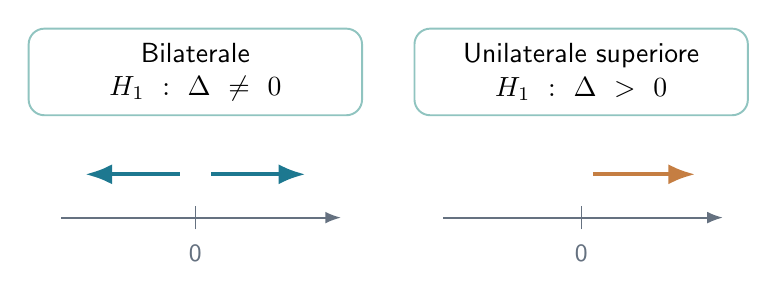
\begin{tikzpicture}[x=1cm,y=1cm]
\node[pFlow,text width=4.0cm] at(2.3,2.75){Bilaterale\\$H_1:\Delta\ne0$};
\node[pFlow,text width=4.0cm] at(7.2,2.75){Unilaterale superiore\\$H_1:\Delta>0$};
\draw[pAxis](.6,.9)--(4.15,.9);
\draw[pAxis](5.45,.9)--(9,.9);
\foreach \x in {2.3,7.2}{
\draw[Muted](\x,.75)--(\x,1.05);
\node[pNote] at(\x,.45){0};}
\draw[GeoA,line width=1.5pt,-{Latex}](2.1,1.45)--(.9,1.45);
\draw[GeoA,line width=1.5pt,-{Latex}](2.5,1.45)--(3.7,1.45);
\draw[GeoB,line width=1.5pt,-{Latex}](7.35,1.45)--(8.65,1.45);
\end{tikzpicture}
\PSmall{La direzione dipende dalla domanda. Le condizioni sulla distribuzione e sul disegno completano il modello sotto cui il test è calibrato.}

\end{minipage}% 
\end{lrbox}
\typeout{FULLBOX:011:L:\the\ht\PilotLeftBox:\the\dp\PilotLeftBox}
\begin{lrbox}{\PilotRightBox}%
\begin{minipage}[t]{7.55cm}\raggedright\color{Ink}\fontsize{11.3}{14.8}\selectfont

\PCode{R · specificare l’alternativa}{011_ipotesi.R}
\PSmall{\texttt{mu=0} indica il contrasto ipotizzato. Con \texttt{t.test(b,a)}, \texttt{"greater"} si riferisce alla media di B maggiore di quella di A.}
\PInfo{Scegliere una coda dopo aver osservato il segno modifica la procedura e il suo controllo dell’errore.}

\end{minipage}% 
\end{lrbox}
\typeout{FULLBOX:011:R:\the\ht\PilotRightBox:\the\dp\PilotRightBox}
\begin{frame}[plain]\hypertarget{slide11}{}
\bookmark[level=1,page=11]{Dichiarare ipotesi e direzione del confronto}
\begin{tikzpicture}[remember picture,overlay]
\PilotChrome{Dichiarare ipotesi e direzione del confronto}{I · DEFINIRE IL CONFRONTO}{11}{Il valore nullo, la direzione e il metodo si definiscono prima di usare il risultato per sostenere una conclusione.}
\node[anchor=north west,inner sep=0] at ([xshift=0.96cm,yshift=-2.13cm]current page.north west) {\usebox{\PilotLeftBox}};
\node[anchor=north west,inner sep=0] at ([xshift=11.52cm,yshift=-2.13cm]current page.north west) {\usebox{\PilotRightBox}};

\end{tikzpicture}\end{frame}

% SLIDE 012 | Quando le etichette sono scambiabili
\begin{lrbox}{\PilotLeftBox}%
\begin{minipage}[t]{10.05cm}\raggedright\color{Ink}\fontsize{11.3}{14.8}\selectfont

\PLabel{La giustificazione della permutazione}
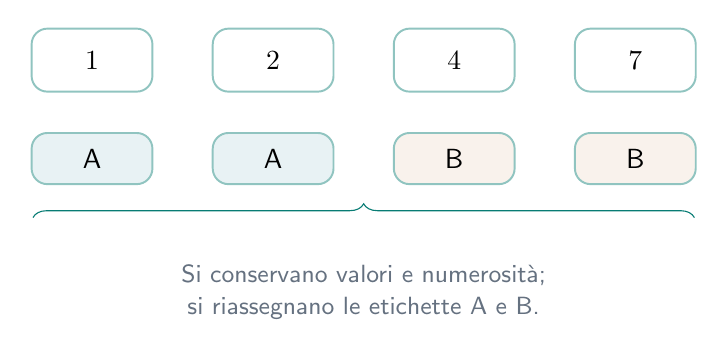
\begin{tikzpicture}[x=1cm,y=1cm]
\foreach \x/\v/\g/\col in {1.3/1/A/GeoA,3.6/2/A/GeoA,5.9/4/B/GeoB,8.2/7/B/GeoB}{
\node[pFlow,text width=1.3cm,minimum height=.8cm] at(\x,3.55){$\v$};
\node[pFlow,fill=\col!10,text width=1.3cm,minimum height=.65cm] at(\x,2.3){\g};
}
\draw[decorate,decoration={brace,amplitude=5pt},Classical](.55,1.55)--(8.95,1.55);
\node[pNote,text width=8.3cm] at(4.75,.6){Si conservano valori e numerosità;\\si riassegnano le etichette A e B.};
\end{tikzpicture}
\PBody{Per campioni IID dalla stessa distribuzione, sotto $H_0$ le etichette non distinguono i valori. Anche una randomizzazione nota può fornire le assegnazioni ammesse.}

\end{minipage}% 
\end{lrbox}
\typeout{FULLBOX:012:L:\the\ht\PilotLeftBox:\the\dp\PilotLeftBox}
\begin{lrbox}{\PilotRightBox}%
\begin{minipage}[t]{7.55cm}\raggedright\color{Ink}\fontsize{11.3}{14.8}\selectfont

\PCode{R · riassegnare i gruppi}{012_etichette.R}
\PSmall{\texttt{sample(g12)} riordina il vettore senza rimpiazzo: restano due A e due B.}
\PInfo{L’uguaglianza delle sole medie non assicura la scambiabilità se cambiano dispersione o forma. La permutazione libera va giustificata.}

\end{minipage}% 
\end{lrbox}
\typeout{FULLBOX:012:R:\the\ht\PilotRightBox:\the\dp\PilotRightBox}
\begin{frame}[plain]\hypertarget{slide12}{}
\bookmark[level=1,page=12]{Quando le etichette sono scambiabili}
\begin{tikzpicture}[remember picture,overlay]
\PilotChrome{Quando le etichette sono scambiabili}{I · DEFINIRE IL CONFRONTO}{12}{La validità di una permutazione deriva dalle assegnazioni ammesse dal modello o dal disegno, non dalla disponibilità del comando sample().}
\node[anchor=north west,inner sep=0] at ([xshift=0.96cm,yshift=-2.13cm]current page.north west) {\usebox{\PilotLeftBox}};
\node[anchor=north west,inner sep=0] at ([xshift=11.52cm,yshift=-2.13cm]current page.north west) {\usebox{\PilotRightBox}};

\end{tikzpicture}\end{frame}

% SLIDE 013 | Quattro valori, sei assegnazioni distinte
\begin{lrbox}{\PilotLeftBox}%
\begin{minipage}[t]{10.05cm}\raggedright\color{Ink}\fontsize{11.3}{14.8}\selectfont

\PLabel{Enumerare tutto il riferimento}
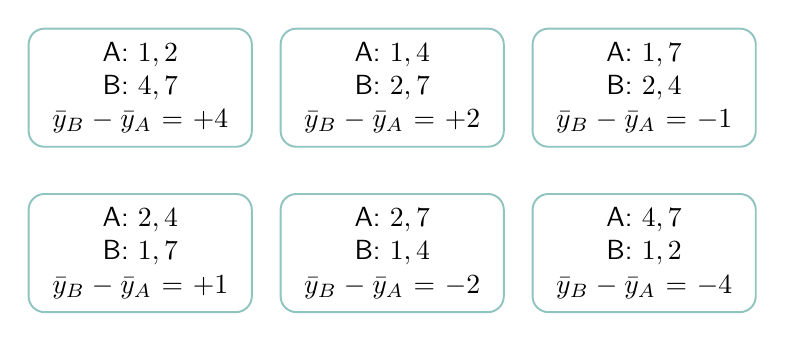
\begin{tikzpicture}[x=1cm,y=1cm]
\foreach \x/\y/\aa/\bb/\tt in {
1.6/3.3/{1,2}/{4,7}/{+4},
4.8/3.3/{1,4}/{2,7}/{+2},
8.0/3.3/{1,7}/{2,4}/{-1},
1.6/1.2/{2,4}/{1,7}/{+1},
4.8/1.2/{2,7}/{1,4}/{-2},
8.0/1.2/{4,7}/{1,2}/{-4}}{
\node[pFlow,text width=2.6cm,minimum height=1.5cm] at(\x,\y)
{A: $\aa$\\B: $\bb$\\$\bar y_B-\bar y_A=\tt$};
}
\end{tikzpicture}
\[
N=\binom42=6,\qquad p_{\mathrm{esatto}}=\frac26
\quad\text{per }|T_{\mathrm{oss}}|=4.
\]
\PSmall{Ogni assegnazione ha lo stesso peso sotto il riferimento dichiarato. Si contano entrambe le direzioni.}

\end{minipage}% 
\end{lrbox}
\typeout{FULLBOX:013:L:\the\ht\PilotLeftBox:\the\dp\PilotLeftBox}
\begin{lrbox}{\PilotRightBox}%
\begin{minipage}[t]{7.55cm}\raggedright\color{Ink}\fontsize{11.3}{14.8}\selectfont

\PCode{R · tutte le combinazioni}{013_sei_assegnazioni.R}
\PSmall{\texttt{combn(4,2)} elenca i possibili indici di A. Il segno meno in \texttt{x13[-i]} seleziona gli indici rimasti per B.}
\PInfo{Questa è un’enumerazione completa. La formula Monte Carlo con $+1$ servirà quando estraiamo soltanto un insieme di permutazioni.}

\end{minipage}% 
\end{lrbox}
\typeout{FULLBOX:013:R:\the\ht\PilotRightBox:\the\dp\PilotRightBox}
\begin{frame}[plain]\hypertarget{slide13}{}
\bookmark[level=1,page=13]{Quattro valori, sei assegnazioni distinte}
\begin{tikzpicture}[remember picture,overlay]
\PilotChrome{Quattro valori, sei assegnazioni distinte}{I · DEFINIRE IL CONFRONTO}{13}{Un riferimento esatto può essere costruito enumerando tutte le assegnazioni ammesse e contando i risultati almeno altrettanto estremi.}
\node[anchor=north west,inner sep=0] at ([xshift=0.96cm,yshift=-2.13cm]current page.north west) {\usebox{\PilotLeftBox}};
\node[anchor=north west,inner sep=0] at ([xshift=11.52cm,yshift=-2.13cm]current page.north west) {\usebox{\PilotRightBox}};

\end{tikzpicture}\end{frame}

% SLIDE 014 | Seguire una singola riassegnazione
\begin{lrbox}{\PilotLeftBox}%
\begin{minipage}[t]{10.05cm}\raggedright\color{Ink}\fontsize{11.3}{14.8}\selectfont

\PLabel{Valori invariati, appartenenza diversa}
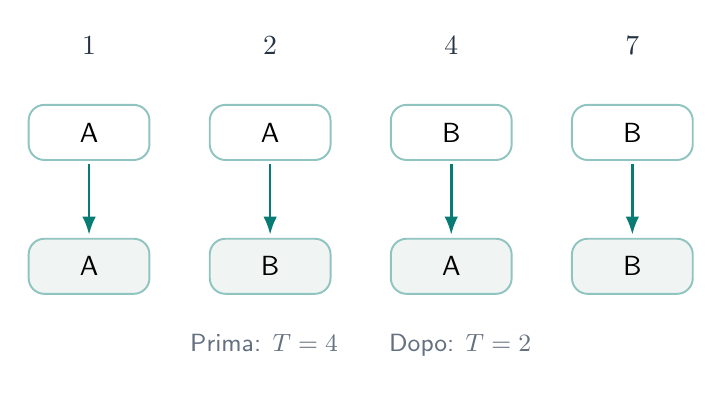
\begin{tikzpicture}[x=1cm,y=1cm]
\foreach \x/\v/\g/\gp in {1.3/1/A/A,3.6/2/A/B,5.9/4/B/A,8.2/7/B/B}{
\node[pLabel] at(\x,4.3){$\v$};
\node[pFlow,text width=1.3cm,minimum height=.7cm] at(\x,3.2){\g};
\node[pFlow,text width=1.3cm,minimum height=.7cm,fill=GeoTint] at(\x,1.5){\gp};
}
\foreach \x in {1.3,3.6,5.9,8.2}\draw[pEdge](\x,2.8)--(\x,1.9);
\node[pNote] at(4.75,.5){Prima: $T=4$\qquad Dopo: $T=2$};
\end{tikzpicture}
\PSmall{Nel secondo assetto A contiene 1 e 4, B contiene 2 e 7. Si applica la stessa statistica a una diversa assegnazione.}

\end{minipage}% 
\end{lrbox}
\typeout{FULLBOX:014:L:\the\ht\PilotLeftBox:\the\dp\PilotLeftBox}
\begin{lrbox}{\PilotRightBox}%
\begin{minipage}[t]{7.55cm}\raggedright\color{Ink}\fontsize{11.3}{14.8}\selectfont

\PCode{R · ricalcolare la statistica}{014_una_permutazione.R}
\PSmall{\texttt{tapply()} calcola le medie seguendo i gruppi. Con i nomi A e B, \texttt{diff()} restituisce B meno A.}
\PInfo{Mantenere una statistica e un ordine fissi evita che il significato del confronto cambi fra le permutazioni.}

\end{minipage}% 
\end{lrbox}
\typeout{FULLBOX:014:R:\the\ht\PilotRightBox:\the\dp\PilotRightBox}
\begin{frame}[plain]\hypertarget{slide14}{}
\bookmark[level=1,page=14]{Seguire una singola riassegnazione}
\begin{tikzpicture}[remember picture,overlay]
\PilotChrome{Seguire una singola riassegnazione}{I · DEFINIRE IL CONFRONTO}{14}{La permutazione modifica le etichette; la regola di calcolo del contrasto rimane identica.}
\node[anchor=north west,inner sep=0] at ([xshift=0.96cm,yshift=-2.13cm]current page.north west) {\usebox{\PilotLeftBox}};
\node[anchor=north west,inner sep=0] at ([xshift=11.52cm,yshift=-2.13cm]current page.north west) {\usebox{\PilotRightBox}};

\end{tikzpicture}\end{frame}

% SLIDE 015 | Ripetere la riassegnazione delle etichette
\begin{lrbox}{\PilotLeftBox}%
\begin{minipage}[t]{10.05cm}\raggedright\color{Ink}\fontsize{11.3}{14.8}\selectfont
\PLabel{Il generatore del laboratorio di permutazione}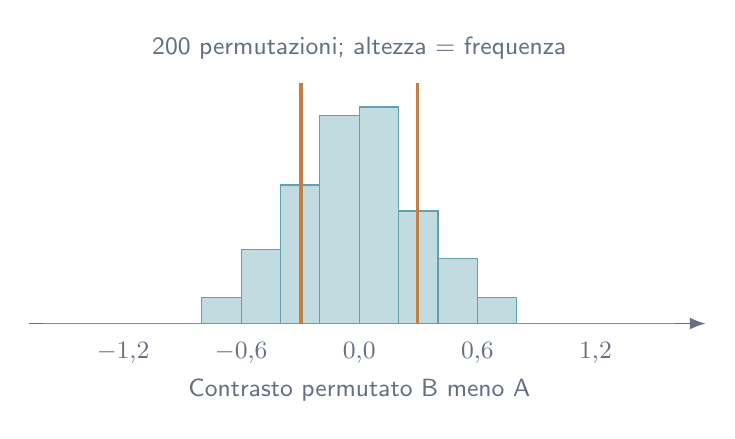
\begin{tikzpicture}[x=1cm,y=1cm]
\draw[pAxis](.6,.5)--(9.2,.5);
\draw[GeoA!70,fill=GeoA!27](0.800,.5) rectangle(1.300,0.500);
\draw[GeoA!70,fill=GeoA!27](1.300,.5) rectangle(1.800,0.500);
\draw[GeoA!70,fill=GeoA!27](1.800,.5) rectangle(2.300,0.500);
\draw[GeoA!70,fill=GeoA!27](2.300,.5) rectangle(2.800,0.500);
\draw[GeoA!70,fill=GeoA!27](2.800,.5) rectangle(3.300,0.830);
\draw[GeoA!70,fill=GeoA!27](3.300,.5) rectangle(3.800,1.435);
\draw[GeoA!70,fill=GeoA!27](3.800,.5) rectangle(4.300,2.260);
\draw[GeoA!70,fill=GeoA!27](4.300,.5) rectangle(4.800,3.140);
\draw[GeoA!70,fill=GeoA!27](4.800,.5) rectangle(5.300,3.250);
\draw[GeoA!70,fill=GeoA!27](5.300,.5) rectangle(5.800,1.930);
\draw[GeoA!70,fill=GeoA!27](5.800,.5) rectangle(6.300,1.325);
\draw[GeoA!70,fill=GeoA!27](6.300,.5) rectangle(6.800,0.830);
\draw[GeoA!70,fill=GeoA!27](6.800,.5) rectangle(7.300,0.500);
\draw[GeoA!70,fill=GeoA!27](7.300,.5) rectangle(7.800,0.500);
\draw[GeoA!70,fill=GeoA!27](7.800,.5) rectangle(8.300,0.500);
\draw[GeoA!70,fill=GeoA!27](8.300,.5) rectangle(8.800,0.500);
\node[pNote] at(1.800,.13){$ -1{,}2 $};
\node[pNote] at(3.300,.13){$ -0{,}6 $};
\node[pNote] at(4.800,.13){$ 0{,}0 $};
\node[pNote] at(6.300,.13){$ 0{,}6 $};
\node[pNote] at(7.800,.13){$ 1{,}2 $};
\draw[GeoB,line width=1.2pt](4.0596,.5)--(4.0596,3.55);
\draw[GeoB,line width=1.2pt](5.5404,.5)--(5.5404,3.55);
\node[pNote] at(4.8,4.0){200 permutazioni; altezza = frequenza};
\node[pNote] at(4.8,-.35){Contrasto permutato B meno A};
\end{tikzpicture}
\PSmall{Campione: 20 osservazioni per gruppo, risposta senza unità fisica. Con seme 17 e $\Delta=0{,}6$, il contrasto osservato è $ -0{,}296$. Le linee indicano $\pm|T_{\mathrm{oss}}|$.}

\end{minipage}% 
\end{lrbox}
\typeout{FULLBOX:015:L:\the\ht\PilotLeftBox:\the\dp\PilotLeftBox}
\begin{lrbox}{\PilotRightBox}%
\begin{minipage}[t]{7.55cm}\raggedright\color{Ink}\fontsize{11.3}{14.8}\selectfont

\PCode{R · 200 contrasti sotto il riferimento}{015_molte_permutazioni.R}
\PSmall{\texttt{replicate()} cambia le etichette dei 40 valori generati una sola volta.}
\PInfo{Parametro e stima possono avere segni diversi in un singolo campione.}

\end{minipage}% 
\end{lrbox}
\typeout{FULLBOX:015:R:\the\ht\PilotRightBox:\the\dp\PilotRightBox}
\begin{frame}[plain]\hypertarget{slide15}{}
\bookmark[level=1,page=15]{Ripetere la riassegnazione delle etichette}
\begin{tikzpicture}[remember picture,overlay]
\PilotChrome{Ripetere la riassegnazione delle etichette}{I · DEFINIRE IL CONFRONTO}{15}{Le permutazioni descrivono il riferimento condizionato ai dati osservati. Aumentarle non aggiunge nuove osservazioni al campione.}
\node[anchor=north west,inner sep=0] at ([xshift=0.96cm,yshift=-2.13cm]current page.north west) {\usebox{\PilotLeftBox}};
\node[anchor=north west,inner sep=0] at ([xshift=11.52cm,yshift=-2.13cm]current page.north west) {\usebox{\PilotRightBox}};

\end{tikzpicture}\end{frame}

% SLIDE 016 | Definire ciò che conta come estremo
\begin{lrbox}{\PilotLeftBox}%
\begin{minipage}[t]{10.05cm}\raggedright\color{Ink}\fontsize{11.3}{14.8}\selectfont

\PLabel{Confronto bilaterale della differenza}
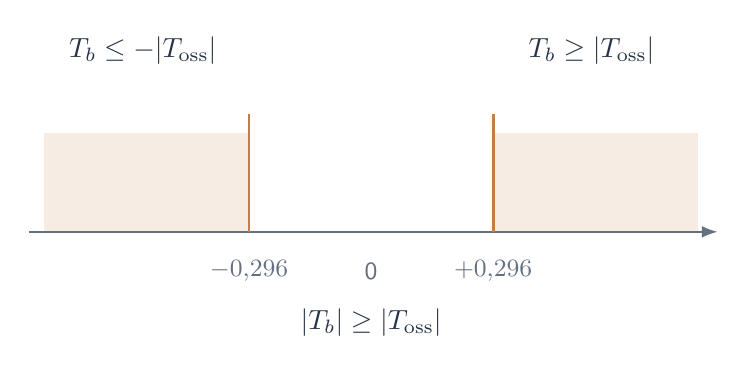
\begin{tikzpicture}[x=1cm,y=1cm]
\fill[GeoB!15](.65,1.2) rectangle(3.25,2.45);
\fill[GeoB!15](6.35,1.2) rectangle(8.95,2.45);
\draw[pAxis](.45,1.2)--(9.2,1.2);
\draw[GeoB,line width=1pt](3.25,1.2)--(3.25,2.7);
\draw[GeoB,line width=1pt](6.35,1.2)--(6.35,2.7);
\node[pLabel] at(1.9,3.5){$T_b\le-|T_{\rm oss}|$};
\node[pLabel] at(7.6,3.5){$T_b\ge|T_{\rm oss}|$};
\node[pNote] at(3.25,.7){$-0{,}296$};
\node[pNote] at(6.35,.7){$+0{,}296$};
\node[pNote] at(4.8,.7){0};
\node[pLabel] at(4.8,.05){$|T_b|\ge|T_{\rm oss}|$};
\end{tikzpicture}
\PSmall{Schema della regola, asse non in scala. Nel campione precedente $ 66$ dei $ 200$ contrasti permutati raggiungono o superano la soglia.}

\end{minipage}% 
\end{lrbox}
\typeout{FULLBOX:016:L:\the\ht\PilotLeftBox:\the\dp\PilotLeftBox}
\begin{lrbox}{\PilotRightBox}%
\begin{minipage}[t]{7.55cm}\raggedright\color{Ink}\fontsize{11.3}{14.8}\selectfont

\PCode{R · contare entrambe le code}{016_estremita.R}
\PSmall{\texttt{abs()} elimina il segno; \texttt{>=} include anche le uguaglianze. La somma dei valori logici conta i risultati che soddisfano la regola.}
\PInfo{Una regola di estremità deve essere fissata e applicata allo stesso modo al dato osservato e a tutte le riassegnazioni.}

\end{minipage}% 
\end{lrbox}
\typeout{FULLBOX:016:R:\the\ht\PilotRightBox:\the\dp\PilotRightBox}
\begin{frame}[plain]\hypertarget{slide16}{}
\bookmark[level=1,page=16]{Definire ciò che conta come estremo}
\begin{tikzpicture}[remember picture,overlay]
\PilotChrome{Definire ciò che conta come estremo}{I · DEFINIRE IL CONFRONTO}{16}{Nel confronto bilaterale con differenza di medie sono estremi i contrasti grandi in valore assoluto, in entrambe le direzioni.}
\node[anchor=north west,inner sep=0] at ([xshift=0.96cm,yshift=-2.13cm]current page.north west) {\usebox{\PilotLeftBox}};
\node[anchor=north west,inner sep=0] at ([xshift=11.52cm,yshift=-2.13cm]current page.north west) {\usebox{\PilotRightBox}};

\end{tikzpicture}\end{frame}

% SLIDE 017 | Il p-value Monte Carlo e la risoluzione
\begin{lrbox}{\PilotLeftBox}%
\begin{minipage}[t]{10.05cm}\raggedright\color{Ink}\fontsize{11.3}{14.8}\selectfont

\PLabel{Un conteggio finito di permutazioni}
\[
p_{MC}=\frac{1+\sum_{b=1}^B
\mathbf1(|T_b|\ge|T_{\mathrm{oss}}|)}{B+1}
=\frac{1+66}{200+1}=0{,}333.
\]
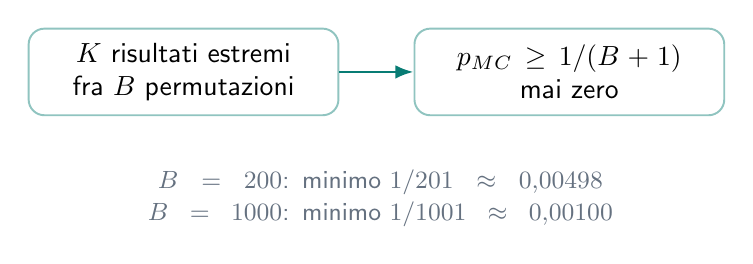
\begin{tikzpicture}[x=1cm,y=1cm]
\node[pFlow,text width=3.7cm] (k) at(2.2,2.4){$K$ risultati estremi\\fra $B$ permutazioni};
\node[pFlow,text width=3.7cm] (p) at(7.1,2.4){$p_{MC}\ge1/(B+1)$\\mai zero};
\draw[pEdge](k)--(p);
\node[pNote,text width=8.5cm] at(4.7,.8){$B=200$: minimo $1/201\approx0{,}00498$\\$B=1000$: minimo $1/1001\approx0{,}00100$};
\end{tikzpicture}
\PSmall{$B$ conta permutazioni estratte; $K$ conta quelle almeno altrettanto estreme. La validità richiede il riferimento di permutazione già giustificato.}

\end{minipage}% 
\end{lrbox}
\typeout{FULLBOX:017:L:\the\ht\PilotLeftBox:\the\dp\PilotLeftBox}
\begin{lrbox}{\PilotRightBox}%
\begin{minipage}[t]{7.55cm}\raggedright\color{Ink}\fontsize{11.3}{14.8}\selectfont

\PCode{R · calcolare senza restituire zero}{017_p_monte_carlo.R}
\PSmall{Aumentando $B$ si raffina il calcolo sullo stesso campione. La variazione Monte Carlo va distinta dalla variabilità fra nuovi campioni.}
\PInfo{Con permutazioni indipendenti, $q$ è la probabilità di coda nel riferimento fissato; l’errore Monte Carlo ha scala circa $\sqrt{q(1-q)/B}$.}

\end{minipage}% 
\end{lrbox}
\typeout{FULLBOX:017:R:\the\ht\PilotRightBox:\the\dp\PilotRightBox}
\begin{frame}[plain]\hypertarget{slide17}{}
\bookmark[level=1,page=17]{Il p-value Monte Carlo e la risoluzione}
\begin{tikzpicture}[remember picture,overlay]
\PilotChrome{Il p-value Monte Carlo e la risoluzione}{I · DEFINIRE IL CONFRONTO}{17}{Nessun estremo osservato in un insieme finito di permutazioni non equivale a probabilità nulla.}
\node[anchor=north west,inner sep=0] at ([xshift=0.96cm,yshift=-2.13cm]current page.north west) {\usebox{\PilotLeftBox}};
\node[anchor=north west,inner sep=0] at ([xshift=11.52cm,yshift=-2.13cm]current page.north west) {\usebox{\PilotRightBox}};

\end{tikzpicture}\end{frame}

% SLIDE 018 | Bootstrap e permutazione hanno scopi diversi
\begin{lrbox}{\PilotLeftBox}%
\begin{minipage}[t]{10.05cm}\raggedright\color{Ink}\fontsize{11.3}{14.8}\selectfont

\PLabel{Quali elementi cambiano?}
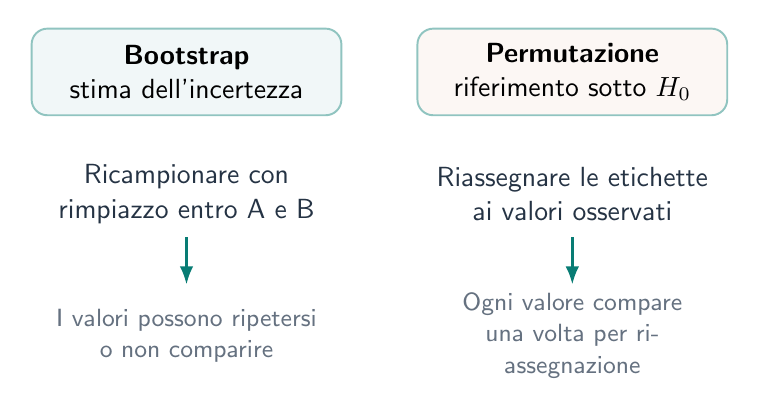
\begin{tikzpicture}[x=1cm,y=1cm]
\node[pFlow,text width=3.7cm,fill=GeoA!6] at(2.2,3.9){\textbf{Bootstrap}\\stima dell’incertezza};
\node[pFlow,text width=3.7cm,fill=GeoB!6] at(7.1,3.9){\textbf{Permutazione}\\riferimento sotto $H_0$};
\node[pLabel,text width=3.7cm] at(2.2,2.35){Ricampionare con\\rimpiazzo entro A e B};
\node[pLabel,text width=3.7cm] at(7.1,2.35){Riassegnare le etichette\\ai valori osservati};
\draw[pEdge](2.2,1.8)--(2.2,1.2);
\draw[pEdge](7.1,1.8)--(7.1,1.2);
\node[pNote,text width=3.8cm] at(2.2,.55){I valori possono ripetersi\\o non comparire};
\node[pNote,text width=3.8cm] at(7.1,.55){Ogni valore compare\\una volta per riassegnazione};
\end{tikzpicture}
\PSmall{Gli schemi mostrati assumono unità indipendenti. Entrambi i procedimenti devono rispettare il disegno.}

\end{minipage}% 
\end{lrbox}
\typeout{FULLBOX:018:L:\the\ht\PilotLeftBox:\the\dp\PilotLeftBox}
\begin{lrbox}{\PilotRightBox}%
\begin{minipage}[t]{7.55cm}\raggedright\color{Ink}\fontsize{11.3}{14.8}\selectfont

\PCode{R · riconoscere le operazioni}{018_bootstrap_permutazione.R}
\PSmall{\texttt{replace=TRUE} permette ripetizioni nel bootstrap. Per la permutazione delle etichette, il valore predefinito è \texttt{FALSE}.}
\PInfo{Il bootstrap ordinario della differenza non impone automaticamente il contrasto nullo. I due riferimenti non sono intercambiabili.}

\end{minipage}% 
\end{lrbox}
\typeout{FULLBOX:018:R:\the\ht\PilotRightBox:\the\dp\PilotRightBox}
\begin{frame}[plain]\hypertarget{slide18}{}
\bookmark[level=1,page=18]{Bootstrap e permutazione hanno scopi diversi}
\begin{tikzpicture}[remember picture,overlay]
\PilotChrome{Bootstrap e permutazione hanno scopi diversi}{I · DEFINIRE IL CONFRONTO}{18}{Prima di ricampionare occorre precisare se interessa l’incertezza della stima oppure un riferimento sotto l’ipotesi nulla.}
\node[anchor=north west,inner sep=0] at ([xshift=0.96cm,yshift=-2.13cm]current page.north west) {\usebox{\PilotLeftBox}};
\node[anchor=north west,inner sep=0] at ([xshift=11.52cm,yshift=-2.13cm]current page.north west) {\usebox{\PilotRightBox}};

\end{tikzpicture}\end{frame}

% SLIDE 019 | Conservare i vincoli del disegno
\begin{lrbox}{\PilotLeftBox}%
\begin{minipage}[t]{10.05cm}\raggedright\color{Ink}\fontsize{11.3}{14.8}\selectfont

\PLabel{Permutazioni ammesse e unità dell’assegnazione}
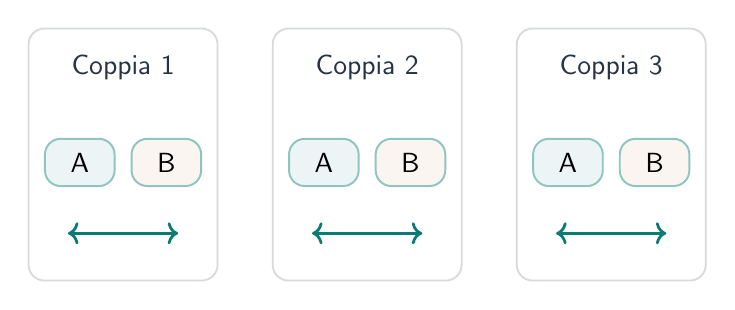
\begin{tikzpicture}[x=1cm,y=1cm]
\foreach \x/\id in {1.7/1,4.8/2,7.9/3}{
\draw[pGroup](\x-1.2,.9) rectangle(\x+1.2,4.1);
\node[pLabel] at(\x,3.6){Coppia \id};
\node[pFlow,fill=GeoA!8,text width=.65cm,minimum height=.6cm] at(\x-.55,2.4){A};
\node[pFlow,fill=GeoB!8,text width=.65cm,minimum height=.6cm] at(\x+.55,2.4){B};
\draw[Classical,<->,line width=1pt](\x-.7,1.5)--(\x+.7,1.5);
}
\end{tikzpicture}
\PSmall{Nelle coppie si può scambiare A e B entro la stessa unità se la randomizzazione lo consente o se il modello nullo giustifica il cambio di segno.}

\end{minipage}% 
\end{lrbox}
\typeout{FULLBOX:019:L:\the\ht\PilotLeftBox:\the\dp\PilotLeftBox}
\begin{lrbox}{\PilotRightBox}%
\begin{minipage}[t]{7.55cm}\raggedright\color{Ink}\fontsize{11.3}{14.8}\selectfont

\PCode{R · una trasformazione entro coppia}{019_vincoli.R}
\PSmall{Moltiplicare $D_i=B_i-A_i$ per $-1$ equivale a invertire A e B nella coppia.}
\PInfo{Per dati osservazionali il cambio di segno richiede, per esempio, differenze indipendenti e simmetriche attorno a zero sotto $H_0$.}

\end{minipage}% 
\end{lrbox}
\typeout{FULLBOX:019:R:\the\ht\PilotRightBox:\the\dp\PilotRightBox}
\begin{frame}[plain]\hypertarget{slide19}{}
\bookmark[level=1,page=19]{Conservare i vincoli del disegno}
\begin{tikzpicture}[remember picture,overlay]
\PilotChrome{Conservare i vincoli del disegno}{I · DEFINIRE IL CONFRONTO}{19}{Coppie, siti e blocchi limitano le trasformazioni ammesse. Una permutazione libera può distruggere la struttura da cui dipende la validità del test.}
\node[anchor=north west,inner sep=0] at ([xshift=0.96cm,yshift=-2.13cm]current page.north west) {\usebox{\PilotLeftBox}};
\node[anchor=north west,inner sep=0] at ([xshift=11.52cm,yshift=-2.13cm]current page.north west) {\usebox{\PilotRightBox}};

\end{tikzpicture}\end{frame}

% SLIDE 020 | Il p-value è un’area nel riferimento
\begin{lrbox}{\PilotLeftBox}%
\begin{minipage}[t]{10.05cm}\raggedright\color{Ink}\fontsize{11.3}{14.8}\selectfont

\PLabel{Due code per una differenza bilaterale}
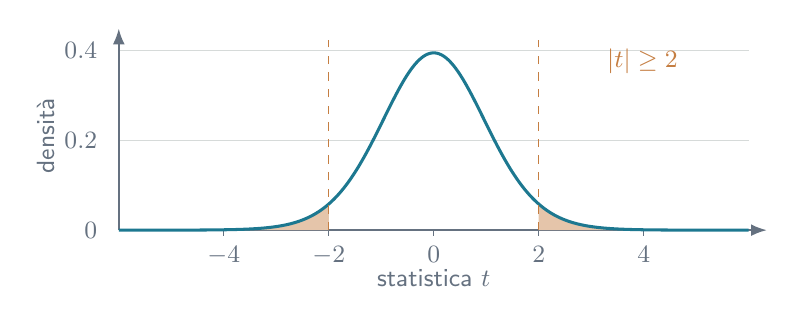
\begin{tikzpicture}[x=1cm,y=1cm]
\draw[Rule](.75,0.0000)--(8.75,0.0000);
\node[pNote,anchor=east] at(.60,0.0000){$ 0 $};
\draw[Rule](.75,1.1429)--(8.75,1.1429);
\node[pNote,anchor=east] at(.60,1.1429){$ 0.2 $};
\draw[Rule](.75,2.2857)--(8.75,2.2857);
\node[pNote,anchor=east] at(.60,2.2857){$ 0.4 $};
\draw[pAxis](.75,0)--(8.98,0);
\draw[pAxis](.75,0)--(.75,2.56);
\draw[Muted](2.0833,0)--(2.0833,-.07);
\node[pNote,below] at(2.0833,-.08){$ -4 $};
\draw[Muted](3.4167,0)--(3.4167,-.07);
\node[pNote,below] at(3.4167,-.08){$ -2 $};
\draw[Muted](4.7500,0)--(4.7500,-.07);
\node[pNote,below] at(4.7500,-.08){$ 0 $};
\draw[Muted](6.0833,0)--(6.0833,-.07);
\node[pNote,below] at(6.0833,-.08){$ 2 $};
\draw[Muted](7.4167,0)--(7.4167,-.07);
\node[pNote,below] at(7.4167,-.08){$ 4 $};
\node[pNote] at(4.75,-.61){statistica $t$};
\node[pNote,rotate=90] at(-.18,1.2){densità};
\fill[GeoB!45] (0.75000,0)-- plot coordinates{(0.75000,0.00005) (0.76333,0.00005) (0.77667,0.00005) (0.79000,0.00005) (0.80333,0.00005) (0.81667,0.00006) (0.83000,0.00006) (0.84333,0.00006) (0.85667,0.00007) (0.87000,0.00007) (0.88333,0.00007) (0.89667,0.00007) (0.91000,0.00008) (0.92333,0.00008) (0.93667,0.00009) (0.95000,0.00009) (0.96333,0.00009) (0.97667,0.00010) (0.99000,0.00010) (1.00333,0.00011) (1.01667,0.00011) (1.03000,0.00012) (1.04333,0.00012) (1.05667,0.00013) (1.07000,0.00014) (1.08333,0.00014) (1.09667,0.00015) (1.11000,0.00016) (1.12333,0.00016) (1.13667,0.00017) (1.15000,0.00018) (1.16333,0.00019) (1.17667,0.00020) (1.19000,0.00020) (1.20333,0.00021) (1.21667,0.00022) (1.23000,0.00024) (1.24333,0.00025) (1.25667,0.00026) (1.27000,0.00027) (1.28333,0.00028) (1.29667,0.00030) (1.31000,0.00031) (1.32333,0.00033) (1.33667,0.00034) (1.35000,0.00036) (1.36333,0.00037) (1.37667,0.00039) (1.39000,0.00041) (1.40333,0.00043) (1.41667,0.00045) (1.43000,0.00047) (1.44333,0.00050) (1.45667,0.00052) (1.47000,0.00054) (1.48333,0.00057) (1.49667,0.00060) (1.51000,0.00063) (1.52333,0.00066) (1.53667,0.00069) (1.55000,0.00072) (1.56333,0.00076) (1.57667,0.00079) (1.59000,0.00083) (1.60333,0.00087) (1.61667,0.00091) (1.63000,0.00095) (1.64333,0.00100) (1.65667,0.00105) (1.67000,0.00110) (1.68333,0.00115) (1.69667,0.00121) (1.71000,0.00126) (1.72333,0.00133) (1.73667,0.00139) (1.75000,0.00146) (1.76333,0.00153) (1.77667,0.00160) (1.79000,0.00168) (1.80333,0.00176) (1.81667,0.00184) (1.83000,0.00193) (1.84333,0.00202) (1.85667,0.00212) (1.87000,0.00222) (1.88333,0.00233) (1.89667,0.00244) (1.91000,0.00256) (1.92333,0.00268) (1.93667,0.00281) (1.95000,0.00294) (1.96333,0.00309) (1.97667,0.00323) (1.99000,0.00339) (2.00333,0.00355) (2.01667,0.00372) (2.03000,0.00390) (2.04333,0.00409) (2.05667,0.00428) (2.07000,0.00449) (2.08333,0.00470) (2.09667,0.00492) (2.11000,0.00516) (2.12333,0.00541) (2.13667,0.00566) (2.15000,0.00593) (2.16333,0.00622) (2.17667,0.00651) (2.19000,0.00682) (2.20333,0.00714) (2.21667,0.00748) (2.23000,0.00784) (2.24333,0.00821) (2.25667,0.00860) (2.27000,0.00900) (2.28333,0.00943) (2.29667,0.00987) (2.31000,0.01034) (2.32333,0.01083) (2.33667,0.01134) (2.35000,0.01187) (2.36333,0.01243) (2.37667,0.01301) (2.39000,0.01362) (2.40333,0.01425) (2.41667,0.01492) (2.43000,0.01561) (2.44333,0.01634) (2.45667,0.01710) (2.47000,0.01789) (2.48333,0.01872) (2.49667,0.01959) (2.51000,0.02049) (2.52333,0.02144) (2.53667,0.02242) (2.55000,0.02345) (2.56333,0.02453) (2.57667,0.02565) (2.59000,0.02682) (2.60333,0.02804) (2.61667,0.02932) (2.63000,0.03065) (2.64333,0.03204) (2.65667,0.03349) (2.67000,0.03500) (2.68333,0.03657) (2.69667,0.03821) (2.71000,0.03993) (2.72333,0.04171) (2.73667,0.04357) (2.75000,0.04551) (2.76333,0.04753) (2.77667,0.04963) (2.79000,0.05182) (2.80333,0.05410) (2.81667,0.05647) (2.83000,0.05894) (2.84333,0.06151) (2.85667,0.06418) (2.87000,0.06697) (2.88333,0.06986) (2.89667,0.07287) (2.91000,0.07600) (2.92333,0.07925) (2.93667,0.08263) (2.95000,0.08614) (2.96333,0.08979) (2.97667,0.09358) (2.99000,0.09752) (3.00333,0.10160) (3.01667,0.10584) (3.03000,0.11024) (3.04333,0.11481) (3.05667,0.11954) (3.07000,0.12445) (3.08333,0.12954) (3.09667,0.13481) (3.11000,0.14028) (3.12333,0.14594) (3.13667,0.15181) (3.15000,0.15788) (3.16333,0.16417) (3.17667,0.17067) (3.19000,0.17740) (3.20333,0.18436) (3.21667,0.19156) (3.23000,0.19900) (3.24333,0.20668) (3.25667,0.21463) (3.27000,0.22283) (3.28333,0.23130) (3.29667,0.24004) (3.31000,0.24906) (3.32333,0.25836) (3.33667,0.26795) (3.35000,0.27784) (3.36333,0.28803) (3.37667,0.29853) (3.39000,0.30934) (3.40333,0.32047) (3.41667,0.33193)}--(3.41667,0)--cycle;
\fill[GeoB!45] (6.08333,0)-- plot coordinates{(6.08333,0.33193) (6.09667,0.32047) (6.11000,0.30934) (6.12333,0.29853) (6.13667,0.28803) (6.15000,0.27784) (6.16333,0.26795) (6.17667,0.25836) (6.19000,0.24906) (6.20333,0.24004) (6.21667,0.23130) (6.23000,0.22283) (6.24333,0.21463) (6.25667,0.20668) (6.27000,0.19900) (6.28333,0.19156) (6.29667,0.18436) (6.31000,0.17740) (6.32333,0.17067) (6.33667,0.16417) (6.35000,0.15788) (6.36333,0.15181) (6.37667,0.14594) (6.39000,0.14028) (6.40333,0.13481) (6.41667,0.12954) (6.43000,0.12445) (6.44333,0.11954) (6.45667,0.11481) (6.47000,0.11024) (6.48333,0.10584) (6.49667,0.10160) (6.51000,0.09752) (6.52333,0.09358) (6.53667,0.08979) (6.55000,0.08614) (6.56333,0.08263) (6.57667,0.07925) (6.59000,0.07600) (6.60333,0.07287) (6.61667,0.06986) (6.63000,0.06697) (6.64333,0.06418) (6.65667,0.06151) (6.67000,0.05894) (6.68333,0.05647) (6.69667,0.05410) (6.71000,0.05182) (6.72333,0.04963) (6.73667,0.04753) (6.75000,0.04551) (6.76333,0.04357) (6.77667,0.04171) (6.79000,0.03993) (6.80333,0.03821) (6.81667,0.03657) (6.83000,0.03500) (6.84333,0.03349) (6.85667,0.03204) (6.87000,0.03065) (6.88333,0.02932) (6.89667,0.02804) (6.91000,0.02682) (6.92333,0.02565) (6.93667,0.02453) (6.95000,0.02345) (6.96333,0.02242) (6.97667,0.02144) (6.99000,0.02049) (7.00333,0.01959) (7.01667,0.01872) (7.03000,0.01789) (7.04333,0.01710) (7.05667,0.01634) (7.07000,0.01561) (7.08333,0.01492) (7.09667,0.01425) (7.11000,0.01362) (7.12333,0.01301) (7.13667,0.01243) (7.15000,0.01187) (7.16333,0.01134) (7.17667,0.01083) (7.19000,0.01034) (7.20333,0.00987) (7.21667,0.00943) (7.23000,0.00900) (7.24333,0.00860) (7.25667,0.00821) (7.27000,0.00784) (7.28333,0.00748) (7.29667,0.00714) (7.31000,0.00682) (7.32333,0.00651) (7.33667,0.00622) (7.35000,0.00593) (7.36333,0.00566) (7.37667,0.00541) (7.39000,0.00516) (7.40333,0.00492) (7.41667,0.00470) (7.43000,0.00449) (7.44333,0.00428) (7.45667,0.00409) (7.47000,0.00390) (7.48333,0.00372) (7.49667,0.00355) (7.51000,0.00339) (7.52333,0.00323) (7.53667,0.00309) (7.55000,0.00294) (7.56333,0.00281) (7.57667,0.00268) (7.59000,0.00256) (7.60333,0.00244) (7.61667,0.00233) (7.63000,0.00222) (7.64333,0.00212) (7.65667,0.00202) (7.67000,0.00193) (7.68333,0.00184) (7.69667,0.00176) (7.71000,0.00168) (7.72333,0.00160) (7.73667,0.00153) (7.75000,0.00146) (7.76333,0.00139) (7.77667,0.00133) (7.79000,0.00126) (7.80333,0.00121) (7.81667,0.00115) (7.83000,0.00110) (7.84333,0.00105) (7.85667,0.00100) (7.87000,0.00095) (7.88333,0.00091) (7.89667,0.00087) (7.91000,0.00083) (7.92333,0.00079) (7.93667,0.00076) (7.95000,0.00072) (7.96333,0.00069) (7.97667,0.00066) (7.99000,0.00063) (8.00333,0.00060) (8.01667,0.00057) (8.03000,0.00054) (8.04333,0.00052) (8.05667,0.00050) (8.07000,0.00047) (8.08333,0.00045) (8.09667,0.00043) (8.11000,0.00041) (8.12333,0.00039) (8.13667,0.00037) (8.15000,0.00036) (8.16333,0.00034) (8.17667,0.00033) (8.19000,0.00031) (8.20333,0.00030) (8.21667,0.00028) (8.23000,0.00027) (8.24333,0.00026) (8.25667,0.00025) (8.27000,0.00024) (8.28333,0.00022) (8.29667,0.00021) (8.31000,0.00020) (8.32333,0.00020) (8.33667,0.00019) (8.35000,0.00018) (8.36333,0.00017) (8.37667,0.00016) (8.39000,0.00016) (8.40333,0.00015) (8.41667,0.00014) (8.43000,0.00014) (8.44333,0.00013) (8.45667,0.00012) (8.47000,0.00012) (8.48333,0.00011) (8.49667,0.00011) (8.51000,0.00010) (8.52333,0.00010) (8.53667,0.00009) (8.55000,0.00009) (8.56333,0.00009) (8.57667,0.00008) (8.59000,0.00008) (8.60333,0.00007) (8.61667,0.00007) (8.63000,0.00007) (8.64333,0.00007) (8.65667,0.00006) (8.67000,0.00006) (8.68333,0.00006) (8.69667,0.00005) (8.71000,0.00005) (8.72333,0.00005) (8.73667,0.00005) (8.75000,0.00005)}--(8.75000,0)--cycle;
\draw[GeoA,line width=1.1pt,] plot coordinates{(0.75000,0.00005) (0.76333,0.00005) (0.77667,0.00005) (0.79000,0.00005) (0.80333,0.00005) (0.81667,0.00006) (0.83000,0.00006) (0.84333,0.00006) (0.85667,0.00007) (0.87000,0.00007) (0.88333,0.00007) (0.89667,0.00007) (0.91000,0.00008) (0.92333,0.00008) (0.93667,0.00009) (0.95000,0.00009) (0.96333,0.00009) (0.97667,0.00010) (0.99000,0.00010) (1.00333,0.00011) (1.01667,0.00011) (1.03000,0.00012) (1.04333,0.00012) (1.05667,0.00013) (1.07000,0.00014) (1.08333,0.00014) (1.09667,0.00015) (1.11000,0.00016) (1.12333,0.00016) (1.13667,0.00017) (1.15000,0.00018) (1.16333,0.00019) (1.17667,0.00020) (1.19000,0.00020) (1.20333,0.00021) (1.21667,0.00022) (1.23000,0.00024) (1.24333,0.00025) (1.25667,0.00026) (1.27000,0.00027) (1.28333,0.00028) (1.29667,0.00030) (1.31000,0.00031) (1.32333,0.00033) (1.33667,0.00034) (1.35000,0.00036) (1.36333,0.00037) (1.37667,0.00039) (1.39000,0.00041) (1.40333,0.00043) (1.41667,0.00045) (1.43000,0.00047) (1.44333,0.00050) (1.45667,0.00052) (1.47000,0.00054) (1.48333,0.00057) (1.49667,0.00060) (1.51000,0.00063) (1.52333,0.00066) (1.53667,0.00069) (1.55000,0.00072) (1.56333,0.00076) (1.57667,0.00079) (1.59000,0.00083) (1.60333,0.00087) (1.61667,0.00091) (1.63000,0.00095) (1.64333,0.00100) (1.65667,0.00105) (1.67000,0.00110) (1.68333,0.00115) (1.69667,0.00121) (1.71000,0.00126) (1.72333,0.00133) (1.73667,0.00139) (1.75000,0.00146) (1.76333,0.00153) (1.77667,0.00160) (1.79000,0.00168) (1.80333,0.00176) (1.81667,0.00184) (1.83000,0.00193) (1.84333,0.00202) (1.85667,0.00212) (1.87000,0.00222) (1.88333,0.00233) (1.89667,0.00244) (1.91000,0.00256) (1.92333,0.00268) (1.93667,0.00281) (1.95000,0.00294) (1.96333,0.00309) (1.97667,0.00323) (1.99000,0.00339) (2.00333,0.00355) (2.01667,0.00372) (2.03000,0.00390) (2.04333,0.00409) (2.05667,0.00428) (2.07000,0.00449) (2.08333,0.00470) (2.09667,0.00492) (2.11000,0.00516) (2.12333,0.00541) (2.13667,0.00566) (2.15000,0.00593) (2.16333,0.00622) (2.17667,0.00651) (2.19000,0.00682) (2.20333,0.00714) (2.21667,0.00748) (2.23000,0.00784) (2.24333,0.00821) (2.25667,0.00860) (2.27000,0.00900) (2.28333,0.00943) (2.29667,0.00987) (2.31000,0.01034) (2.32333,0.01083) (2.33667,0.01134) (2.35000,0.01187) (2.36333,0.01243) (2.37667,0.01301) (2.39000,0.01362) (2.40333,0.01425) (2.41667,0.01492) (2.43000,0.01561) (2.44333,0.01634) (2.45667,0.01710) (2.47000,0.01789) (2.48333,0.01872) (2.49667,0.01959) (2.51000,0.02049) (2.52333,0.02144) (2.53667,0.02242) (2.55000,0.02345) (2.56333,0.02453) (2.57667,0.02565) (2.59000,0.02682) (2.60333,0.02804) (2.61667,0.02932) (2.63000,0.03065) (2.64333,0.03204) (2.65667,0.03349) (2.67000,0.03500) (2.68333,0.03657) (2.69667,0.03821) (2.71000,0.03993) (2.72333,0.04171) (2.73667,0.04357) (2.75000,0.04551) (2.76333,0.04753) (2.77667,0.04963) (2.79000,0.05182) (2.80333,0.05410) (2.81667,0.05647) (2.83000,0.05894) (2.84333,0.06151) (2.85667,0.06418) (2.87000,0.06697) (2.88333,0.06986) (2.89667,0.07287) (2.91000,0.07600) (2.92333,0.07925) (2.93667,0.08263) (2.95000,0.08614) (2.96333,0.08979) (2.97667,0.09358) (2.99000,0.09752) (3.00333,0.10160) (3.01667,0.10584) (3.03000,0.11024) (3.04333,0.11481) (3.05667,0.11954) (3.07000,0.12445) (3.08333,0.12954) (3.09667,0.13481) (3.11000,0.14028) (3.12333,0.14594) (3.13667,0.15181) (3.15000,0.15788) (3.16333,0.16417) (3.17667,0.17067) (3.19000,0.17740) (3.20333,0.18436) (3.21667,0.19156) (3.23000,0.19900) (3.24333,0.20668) (3.25667,0.21463) (3.27000,0.22283) (3.28333,0.23130) (3.29667,0.24004) (3.31000,0.24906) (3.32333,0.25836) (3.33667,0.26795) (3.35000,0.27784) (3.36333,0.28803) (3.37667,0.29853) (3.39000,0.30934) (3.40333,0.32047) (3.41667,0.33193) (3.43000,0.34371) (3.44333,0.35583) (3.45667,0.36828) (3.47000,0.38108) (3.48333,0.39423) (3.49667,0.40773) (3.51000,0.42159) (3.52333,0.43581) (3.53667,0.45040) (3.55000,0.46535) (3.56333,0.48068) (3.57667,0.49637) (3.59000,0.51245) (3.60333,0.52890) (3.61667,0.54573) (3.63000,0.56295) (3.64333,0.58054) (3.65667,0.59852) (3.67000,0.61688) (3.68333,0.63562) (3.69667,0.65475) (3.71000,0.67425) (3.72333,0.69413) (3.73667,0.71439) (3.75000,0.73501) (3.76333,0.75601) (3.77667,0.77737) (3.79000,0.79908) (3.80333,0.82115) (3.81667,0.84357) (3.83000,0.86633) (3.84333,0.88941) (3.85667,0.91283) (3.87000,0.93655) (3.88333,0.96058) (3.89667,0.98491) (3.91000,1.00952) (3.92333,1.03440) (3.93667,1.05954) (3.95000,1.08493) (3.96333,1.11054) (3.97667,1.13638) (3.99000,1.16241) (4.00333,1.18863) (4.01667,1.21502) (4.03000,1.24156) (4.04333,1.26823) (4.05667,1.29501) (4.07000,1.32188) (4.08333,1.34883) (4.09667,1.37583) (4.11000,1.40286) (4.12333,1.42990) (4.13667,1.45692) (4.15000,1.48390) (4.16333,1.51082) (4.17667,1.53765) (4.19000,1.56437) (4.20333,1.59095) (4.21667,1.61737) (4.23000,1.64360) (4.24333,1.66961) (4.25667,1.69539) (4.27000,1.72089) (4.28333,1.74610) (4.29667,1.77099) (4.31000,1.79553) (4.32333,1.81969) (4.33667,1.84345) (4.35000,1.86678) (4.36333,1.88966) (4.37667,1.91205) (4.39000,1.93392) (4.40333,1.95527) (4.41667,1.97605) (4.43000,1.99624) (4.44333,2.01583) (4.45667,2.03477) (4.47000,2.05306) (4.48333,2.07067) (4.49667,2.08757) (4.51000,2.10374) (4.52333,2.11916) (4.53667,2.13382) (4.55000,2.14769) (4.56333,2.16075) (4.57667,2.17299) (4.59000,2.18440) (4.60333,2.19494) (4.61667,2.20462) (4.63000,2.21342) (4.64333,2.22133) (4.65667,2.22833) (4.67000,2.23441) (4.68333,2.23958) (4.69667,2.24381) (4.71000,2.24711) (4.72333,2.24947) (4.73667,2.25089) (4.75000,2.25136) (4.76333,2.25089) (4.77667,2.24947) (4.79000,2.24711) (4.80333,2.24381) (4.81667,2.23958) (4.83000,2.23441) (4.84333,2.22833) (4.85667,2.22133) (4.87000,2.21342) (4.88333,2.20462) (4.89667,2.19494) (4.91000,2.18440) (4.92333,2.17299) (4.93667,2.16075) (4.95000,2.14769) (4.96333,2.13382) (4.97667,2.11916) (4.99000,2.10374) (5.00333,2.08757) (5.01667,2.07067) (5.03000,2.05306) (5.04333,2.03477) (5.05667,2.01583) (5.07000,1.99624) (5.08333,1.97605) (5.09667,1.95527) (5.11000,1.93392) (5.12333,1.91205) (5.13667,1.88966) (5.15000,1.86678) (5.16333,1.84345) (5.17667,1.81969) (5.19000,1.79553) (5.20333,1.77099) (5.21667,1.74610) (5.23000,1.72089) (5.24333,1.69539) (5.25667,1.66961) (5.27000,1.64360) (5.28333,1.61737) (5.29667,1.59095) (5.31000,1.56437) (5.32333,1.53765) (5.33667,1.51082) (5.35000,1.48390) (5.36333,1.45692) (5.37667,1.42990) (5.39000,1.40286) (5.40333,1.37583) (5.41667,1.34883) (5.43000,1.32188) (5.44333,1.29501) (5.45667,1.26823) (5.47000,1.24156) (5.48333,1.21502) (5.49667,1.18863) (5.51000,1.16241) (5.52333,1.13638) (5.53667,1.11054) (5.55000,1.08493) (5.56333,1.05954) (5.57667,1.03440) (5.59000,1.00952) (5.60333,0.98491) (5.61667,0.96058) (5.63000,0.93655) (5.64333,0.91283) (5.65667,0.88941) (5.67000,0.86633) (5.68333,0.84357) (5.69667,0.82115) (5.71000,0.79908) (5.72333,0.77737) (5.73667,0.75601) (5.75000,0.73501) (5.76333,0.71439) (5.77667,0.69413) (5.79000,0.67425) (5.80333,0.65475) (5.81667,0.63562) (5.83000,0.61688) (5.84333,0.59852) (5.85667,0.58054) (5.87000,0.56295) (5.88333,0.54573) (5.89667,0.52890) (5.91000,0.51245) (5.92333,0.49637) (5.93667,0.48068) (5.95000,0.46535) (5.96333,0.45040) (5.97667,0.43581) (5.99000,0.42159) (6.00333,0.40773) (6.01667,0.39423) (6.03000,0.38108) (6.04333,0.36828) (6.05667,0.35583) (6.07000,0.34371) (6.08333,0.33193) (6.09667,0.32047) (6.11000,0.30934) (6.12333,0.29853) (6.13667,0.28803) (6.15000,0.27784) (6.16333,0.26795) (6.17667,0.25836) (6.19000,0.24906) (6.20333,0.24004) (6.21667,0.23130) (6.23000,0.22283) (6.24333,0.21463) (6.25667,0.20668) (6.27000,0.19900) (6.28333,0.19156) (6.29667,0.18436) (6.31000,0.17740) (6.32333,0.17067) (6.33667,0.16417) (6.35000,0.15788) (6.36333,0.15181) (6.37667,0.14594) (6.39000,0.14028) (6.40333,0.13481) (6.41667,0.12954) (6.43000,0.12445) (6.44333,0.11954) (6.45667,0.11481) (6.47000,0.11024) (6.48333,0.10584) (6.49667,0.10160) (6.51000,0.09752) (6.52333,0.09358) (6.53667,0.08979) (6.55000,0.08614) (6.56333,0.08263) (6.57667,0.07925) (6.59000,0.07600) (6.60333,0.07287) (6.61667,0.06986) (6.63000,0.06697) (6.64333,0.06418) (6.65667,0.06151) (6.67000,0.05894) (6.68333,0.05647) (6.69667,0.05410) (6.71000,0.05182) (6.72333,0.04963) (6.73667,0.04753) (6.75000,0.04551) (6.76333,0.04357) (6.77667,0.04171) (6.79000,0.03993) (6.80333,0.03821) (6.81667,0.03657) (6.83000,0.03500) (6.84333,0.03349) (6.85667,0.03204) (6.87000,0.03065) (6.88333,0.02932) (6.89667,0.02804) (6.91000,0.02682) (6.92333,0.02565) (6.93667,0.02453) (6.95000,0.02345) (6.96333,0.02242) (6.97667,0.02144) (6.99000,0.02049) (7.00333,0.01959) (7.01667,0.01872) (7.03000,0.01789) (7.04333,0.01710) (7.05667,0.01634) (7.07000,0.01561) (7.08333,0.01492) (7.09667,0.01425) (7.11000,0.01362) (7.12333,0.01301) (7.13667,0.01243) (7.15000,0.01187) (7.16333,0.01134) (7.17667,0.01083) (7.19000,0.01034) (7.20333,0.00987) (7.21667,0.00943) (7.23000,0.00900) (7.24333,0.00860) (7.25667,0.00821) (7.27000,0.00784) (7.28333,0.00748) (7.29667,0.00714) (7.31000,0.00682) (7.32333,0.00651) (7.33667,0.00622) (7.35000,0.00593) (7.36333,0.00566) (7.37667,0.00541) (7.39000,0.00516) (7.40333,0.00492) (7.41667,0.00470) (7.43000,0.00449) (7.44333,0.00428) (7.45667,0.00409) (7.47000,0.00390) (7.48333,0.00372) (7.49667,0.00355) (7.51000,0.00339) (7.52333,0.00323) (7.53667,0.00309) (7.55000,0.00294) (7.56333,0.00281) (7.57667,0.00268) (7.59000,0.00256) (7.60333,0.00244) (7.61667,0.00233) (7.63000,0.00222) (7.64333,0.00212) (7.65667,0.00202) (7.67000,0.00193) (7.68333,0.00184) (7.69667,0.00176) (7.71000,0.00168) (7.72333,0.00160) (7.73667,0.00153) (7.75000,0.00146) (7.76333,0.00139) (7.77667,0.00133) (7.79000,0.00126) (7.80333,0.00121) (7.81667,0.00115) (7.83000,0.00110) (7.84333,0.00105) (7.85667,0.00100) (7.87000,0.00095) (7.88333,0.00091) (7.89667,0.00087) (7.91000,0.00083) (7.92333,0.00079) (7.93667,0.00076) (7.95000,0.00072) (7.96333,0.00069) (7.97667,0.00066) (7.99000,0.00063) (8.00333,0.00060) (8.01667,0.00057) (8.03000,0.00054) (8.04333,0.00052) (8.05667,0.00050) (8.07000,0.00047) (8.08333,0.00045) (8.09667,0.00043) (8.11000,0.00041) (8.12333,0.00039) (8.13667,0.00037) (8.15000,0.00036) (8.16333,0.00034) (8.17667,0.00033) (8.19000,0.00031) (8.20333,0.00030) (8.21667,0.00028) (8.23000,0.00027) (8.24333,0.00026) (8.25667,0.00025) (8.27000,0.00024) (8.28333,0.00022) (8.29667,0.00021) (8.31000,0.00020) (8.32333,0.00020) (8.33667,0.00019) (8.35000,0.00018) (8.36333,0.00017) (8.37667,0.00016) (8.39000,0.00016) (8.40333,0.00015) (8.41667,0.00014) (8.43000,0.00014) (8.44333,0.00013) (8.45667,0.00012) (8.47000,0.00012) (8.48333,0.00011) (8.49667,0.00011) (8.51000,0.00010) (8.52333,0.00010) (8.53667,0.00009) (8.55000,0.00009) (8.56333,0.00009) (8.57667,0.00008) (8.59000,0.00008) (8.60333,0.00007) (8.61667,0.00007) (8.63000,0.00007) (8.64333,0.00007) (8.65667,0.00006) (8.67000,0.00006) (8.68333,0.00006) (8.69667,0.00005) (8.71000,0.00005) (8.72333,0.00005) (8.73667,0.00005) (8.75000,0.00005)};
\draw[GeoB,dashed](3.4166666666666665,0)--(3.4166666666666665,2.42);
\draw[GeoB,dashed](6.083333333333333,0)--(6.083333333333333,2.42);
\node[pNote,text=GeoB] at(7.4,2.15){$|t|\geq 2$};
\end{tikzpicture}
\[
p=\Pr_{H_0}\!\left(|T|\geq|t_{\mathrm{obs}}|\right).
\]
\PSmall{La probabilità usa il modello nullo, il disegno e la regola di estremità dichiarati. Il grafico mostra $T\sim t_{20}$ e $t_{\mathrm{obs}}=2$.}

\end{minipage}% 
\end{lrbox}
\typeout{FULLBOX:020:L:\the\ht\PilotLeftBox:\the\dp\PilotLeftBox}
\begin{lrbox}{\PilotRightBox}%
\begin{minipage}[t]{7.55cm}\raggedright\color{Ink}\fontsize{11.3}{14.8}\selectfont

\PCode{R · probabilità nelle due code}{020_p_bilaterale.R}
\PBody{\texttt{pt()} è la funzione di ripartizione della distribuzione $t$. La simmetria permette di raddoppiare la coda a sinistra di $-|t_{\mathrm{obs}}|$.}
\PInfo{Qui $p\simeq0{,}0593$. L’area è calcolata sull’intera distribuzione; il disegno visualizza soltanto l’intervallo da $-6$ a $6$.}

\end{minipage}% 
\end{lrbox}
\typeout{FULLBOX:020:R:\the\ht\PilotRightBox:\the\dp\PilotRightBox}
\begin{frame}[plain]\hypertarget{slide20}{}
\bookmark[level=1,page=20]{Il p-value è un’area nel riferimento}
\begin{tikzpicture}[remember picture,overlay]
\PilotChrome{Il p-value è un’area nel riferimento}{II · INTERPRETARE L’EVIDENZA}{20}{Il p-value confronta la statistica osservata con risultati almeno altrettanto estremi sotto il riferimento nullo.}
\node[anchor=north west,inner sep=0] at ([xshift=0.96cm,yshift=-2.13cm]current page.north west) {\usebox{\PilotLeftBox}};
\node[anchor=north west,inner sep=0] at ([xshift=11.52cm,yshift=-2.13cm]current page.north west) {\usebox{\PilotRightBox}};

\end{tikzpicture}\end{frame}

% SLIDE 021 | La statistica richiede un riferimento
\begin{lrbox}{\PilotLeftBox}%
\begin{minipage}[t]{10.05cm}\raggedright\color{Ink}\fontsize{11.3}{14.8}\selectfont

\PLabel{Le code dipendono dai gradi di libertà}
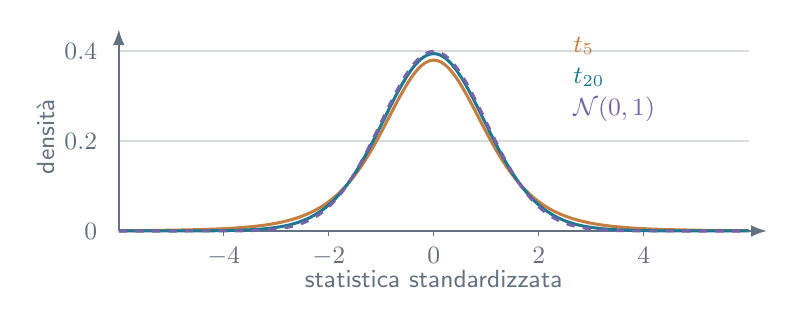
\begin{tikzpicture}[x=1cm,y=1cm]
\draw[Rule](.75,0.0000)--(8.75,0.0000);
\node[pNote,anchor=east] at(.60,0.0000){$ 0 $};
\draw[Rule](.75,1.1429)--(8.75,1.1429);
\node[pNote,anchor=east] at(.60,1.1429){$ 0.2 $};
\draw[Rule](.75,2.2857)--(8.75,2.2857);
\node[pNote,anchor=east] at(.60,2.2857){$ 0.4 $};
\draw[pAxis](.75,0)--(8.98,0);
\draw[pAxis](.75,0)--(.75,2.56);
\draw[Muted](2.0833,0)--(2.0833,-.07);
\node[pNote,below] at(2.0833,-.08){$ -4 $};
\draw[Muted](3.4167,0)--(3.4167,-.07);
\node[pNote,below] at(3.4167,-.08){$ -2 $};
\draw[Muted](4.7500,0)--(4.7500,-.07);
\node[pNote,below] at(4.7500,-.08){$ 0 $};
\draw[Muted](6.0833,0)--(6.0833,-.07);
\node[pNote,below] at(6.0833,-.08){$ 2 $};
\draw[Muted](7.4167,0)--(7.4167,-.07);
\node[pNote,below] at(7.4167,-.08){$ 4 $};
\node[pNote] at(4.75,-.61){statistica standardizzata};
\node[pNote,rotate=90] at(-.18,1.2){densità};
\draw[GeoB,line width=1.1pt,] plot coordinates{(0.75000,0.00393) (0.76333,0.00400) (0.77667,0.00408) (0.79000,0.00415) (0.80333,0.00422) (0.81667,0.00430) (0.83000,0.00437) (0.84333,0.00445) (0.85667,0.00453) (0.87000,0.00462) (0.88333,0.00470) (0.89667,0.00479) (0.91000,0.00487) (0.92333,0.00496) (0.93667,0.00505) (0.95000,0.00515) (0.96333,0.00524) (0.97667,0.00534) (0.99000,0.00544) (1.00333,0.00554) (1.01667,0.00564) (1.03000,0.00575) (1.04333,0.00585) (1.05667,0.00596) (1.07000,0.00608) (1.08333,0.00619) (1.09667,0.00631) (1.11000,0.00643) (1.12333,0.00655) (1.13667,0.00667) (1.15000,0.00680) (1.16333,0.00693) (1.17667,0.00707) (1.19000,0.00720) (1.20333,0.00734) (1.21667,0.00748) (1.23000,0.00763) (1.24333,0.00778) (1.25667,0.00793) (1.27000,0.00809) (1.28333,0.00824) (1.29667,0.00841) (1.31000,0.00857) (1.32333,0.00874) (1.33667,0.00892) (1.35000,0.00909) (1.36333,0.00927) (1.37667,0.00946) (1.39000,0.00965) (1.40333,0.00984) (1.41667,0.01004) (1.43000,0.01025) (1.44333,0.01045) (1.45667,0.01067) (1.47000,0.01088) (1.48333,0.01111) (1.49667,0.01133) (1.51000,0.01157) (1.52333,0.01181) (1.53667,0.01205) (1.55000,0.01230) (1.56333,0.01255) (1.57667,0.01282) (1.59000,0.01308) (1.60333,0.01336) (1.61667,0.01364) (1.63000,0.01393) (1.64333,0.01422) (1.65667,0.01452) (1.67000,0.01483) (1.68333,0.01515) (1.69667,0.01547) (1.71000,0.01580) (1.72333,0.01614) (1.73667,0.01649) (1.75000,0.01684) (1.76333,0.01721) (1.77667,0.01758) (1.79000,0.01796) (1.80333,0.01836) (1.81667,0.01876) (1.83000,0.01917) (1.84333,0.01959) (1.85667,0.02002) (1.87000,0.02047) (1.88333,0.02092) (1.89667,0.02139) (1.91000,0.02186) (1.92333,0.02235) (1.93667,0.02285) (1.95000,0.02337) (1.96333,0.02389) (1.97667,0.02443) (1.99000,0.02499) (2.00333,0.02555) (2.01667,0.02614) (2.03000,0.02673) (2.04333,0.02735) (2.05667,0.02797) (2.07000,0.02862) (2.08333,0.02928) (2.09667,0.02996) (2.11000,0.03065) (2.12333,0.03136) (2.13667,0.03210) (2.15000,0.03285) (2.16333,0.03362) (2.17667,0.03441) (2.19000,0.03522) (2.20333,0.03605) (2.21667,0.03691) (2.23000,0.03778) (2.24333,0.03869) (2.25667,0.03961) (2.27000,0.04056) (2.28333,0.04153) (2.29667,0.04253) (2.31000,0.04356) (2.32333,0.04461) (2.33667,0.04569) (2.35000,0.04680) (2.36333,0.04795) (2.37667,0.04912) (2.39000,0.05032) (2.40333,0.05156) (2.41667,0.05282) (2.43000,0.05413) (2.44333,0.05547) (2.45667,0.05684) (2.47000,0.05826) (2.48333,0.05971) (2.49667,0.06120) (2.51000,0.06273) (2.52333,0.06430) (2.53667,0.06592) (2.55000,0.06758) (2.56333,0.06929) (2.57667,0.07104) (2.59000,0.07285) (2.60333,0.07470) (2.61667,0.07660) (2.63000,0.07856) (2.64333,0.08057) (2.65667,0.08264) (2.67000,0.08476) (2.68333,0.08695) (2.69667,0.08919) (2.71000,0.09150) (2.72333,0.09387) (2.73667,0.09631) (2.75000,0.09881) (2.76333,0.10139) (2.77667,0.10404) (2.79000,0.10676) (2.80333,0.10956) (2.81667,0.11244) (2.83000,0.11540) (2.84333,0.11844) (2.85667,0.12157) (2.87000,0.12478) (2.88333,0.12809) (2.89667,0.13149) (2.91000,0.13498) (2.92333,0.13857) (2.93667,0.14227) (2.95000,0.14607) (2.96333,0.14997) (2.97667,0.15399) (2.99000,0.15811) (3.00333,0.16236) (3.01667,0.16672) (3.03000,0.17120) (3.04333,0.17581) (3.05667,0.18055) (3.07000,0.18543) (3.08333,0.19044) (3.09667,0.19558) (3.11000,0.20088) (3.12333,0.20632) (3.13667,0.21191) (3.15000,0.21766) (3.16333,0.22356) (3.17667,0.22963) (3.19000,0.23587) (3.20333,0.24228) (3.21667,0.24886) (3.23000,0.25563) (3.24333,0.26258) (3.25667,0.26972) (3.27000,0.27706) (3.28333,0.28459) (3.29667,0.29233) (3.31000,0.30028) (3.32333,0.30844) (3.33667,0.31681) (3.35000,0.32541) (3.36333,0.33424) (3.37667,0.34331) (3.39000,0.35261) (3.40333,0.36215) (3.41667,0.37194) (3.43000,0.38199) (3.44333,0.39230) (3.45667,0.40286) (3.47000,0.41370) (3.48333,0.42481) (3.49667,0.43620) (3.51000,0.44787) (3.52333,0.45984) (3.53667,0.47209) (3.55000,0.48465) (3.56333,0.49750) (3.57667,0.51067) (3.59000,0.52414) (3.60333,0.53793) (3.61667,0.55205) (3.63000,0.56648) (3.64333,0.58125) (3.65667,0.59634) (3.67000,0.61177) (3.68333,0.62754) (3.69667,0.64365) (3.71000,0.66010) (3.72333,0.67689) (3.73667,0.69404) (3.75000,0.71153) (3.76333,0.72937) (3.77667,0.74756) (3.79000,0.76610) (3.80333,0.78499) (3.81667,0.80423) (3.83000,0.82381) (3.84333,0.84374) (3.85667,0.86402) (3.87000,0.88463) (3.88333,0.90558) (3.89667,0.92686) (3.91000,0.94847) (3.92333,0.97040) (3.93667,0.99264) (3.95000,1.01519) (3.96333,1.03804) (3.97667,1.06118) (3.99000,1.08459) (4.00333,1.10828) (4.01667,1.13222) (4.03000,1.15641) (4.04333,1.18082) (4.05667,1.20546) (4.07000,1.23029) (4.08333,1.25531) (4.09667,1.28050) (4.11000,1.30584) (4.12333,1.33130) (4.13667,1.35688) (4.15000,1.38254) (4.16333,1.40827) (4.17667,1.43404) (4.19000,1.45983) (4.20333,1.48561) (4.21667,1.51136) (4.23000,1.53705) (4.24333,1.56266) (4.25667,1.58815) (4.27000,1.61349) (4.28333,1.63866) (4.29667,1.66362) (4.31000,1.68835) (4.32333,1.71281) (4.33667,1.73698) (4.35000,1.76081) (4.36333,1.78427) (4.37667,1.80734) (4.39000,1.82997) (4.40333,1.85215) (4.41667,1.87382) (4.43000,1.89496) (4.44333,1.91555) (4.45667,1.93553) (4.47000,1.95489) (4.48333,1.97359) (4.49667,1.99160) (4.51000,2.00889) (4.52333,2.02542) (4.53667,2.04118) (4.55000,2.05614) (4.56333,2.07026) (4.57667,2.08353) (4.59000,2.09591) (4.60333,2.10739) (4.61667,2.11794) (4.63000,2.12755) (4.64333,2.13620) (4.65667,2.14387) (4.67000,2.15055) (4.68333,2.15622) (4.69667,2.16087) (4.71000,2.16450) (4.72333,2.16710) (4.73667,2.16866) (4.75000,2.16918) (4.76333,2.16866) (4.77667,2.16710) (4.79000,2.16450) (4.80333,2.16087) (4.81667,2.15622) (4.83000,2.15055) (4.84333,2.14387) (4.85667,2.13620) (4.87000,2.12755) (4.88333,2.11794) (4.89667,2.10739) (4.91000,2.09591) (4.92333,2.08353) (4.93667,2.07026) (4.95000,2.05614) (4.96333,2.04118) (4.97667,2.02542) (4.99000,2.00889) (5.00333,1.99160) (5.01667,1.97359) (5.03000,1.95489) (5.04333,1.93553) (5.05667,1.91555) (5.07000,1.89496) (5.08333,1.87382) (5.09667,1.85215) (5.11000,1.82997) (5.12333,1.80734) (5.13667,1.78427) (5.15000,1.76081) (5.16333,1.73698) (5.17667,1.71281) (5.19000,1.68835) (5.20333,1.66362) (5.21667,1.63866) (5.23000,1.61349) (5.24333,1.58815) (5.25667,1.56266) (5.27000,1.53705) (5.28333,1.51136) (5.29667,1.48561) (5.31000,1.45983) (5.32333,1.43404) (5.33667,1.40827) (5.35000,1.38254) (5.36333,1.35688) (5.37667,1.33130) (5.39000,1.30584) (5.40333,1.28050) (5.41667,1.25531) (5.43000,1.23029) (5.44333,1.20546) (5.45667,1.18082) (5.47000,1.15641) (5.48333,1.13222) (5.49667,1.10828) (5.51000,1.08459) (5.52333,1.06118) (5.53667,1.03804) (5.55000,1.01519) (5.56333,0.99264) (5.57667,0.97040) (5.59000,0.94847) (5.60333,0.92686) (5.61667,0.90558) (5.63000,0.88463) (5.64333,0.86402) (5.65667,0.84374) (5.67000,0.82381) (5.68333,0.80423) (5.69667,0.78499) (5.71000,0.76610) (5.72333,0.74756) (5.73667,0.72937) (5.75000,0.71153) (5.76333,0.69404) (5.77667,0.67689) (5.79000,0.66010) (5.80333,0.64365) (5.81667,0.62754) (5.83000,0.61177) (5.84333,0.59634) (5.85667,0.58125) (5.87000,0.56648) (5.88333,0.55205) (5.89667,0.53793) (5.91000,0.52414) (5.92333,0.51067) (5.93667,0.49750) (5.95000,0.48465) (5.96333,0.47209) (5.97667,0.45984) (5.99000,0.44787) (6.00333,0.43620) (6.01667,0.42481) (6.03000,0.41370) (6.04333,0.40286) (6.05667,0.39230) (6.07000,0.38199) (6.08333,0.37194) (6.09667,0.36215) (6.11000,0.35261) (6.12333,0.34331) (6.13667,0.33424) (6.15000,0.32541) (6.16333,0.31681) (6.17667,0.30844) (6.19000,0.30028) (6.20333,0.29233) (6.21667,0.28459) (6.23000,0.27706) (6.24333,0.26972) (6.25667,0.26258) (6.27000,0.25563) (6.28333,0.24886) (6.29667,0.24228) (6.31000,0.23587) (6.32333,0.22963) (6.33667,0.22356) (6.35000,0.21766) (6.36333,0.21191) (6.37667,0.20632) (6.39000,0.20088) (6.40333,0.19558) (6.41667,0.19044) (6.43000,0.18543) (6.44333,0.18055) (6.45667,0.17581) (6.47000,0.17120) (6.48333,0.16672) (6.49667,0.16236) (6.51000,0.15811) (6.52333,0.15399) (6.53667,0.14997) (6.55000,0.14607) (6.56333,0.14227) (6.57667,0.13857) (6.59000,0.13498) (6.60333,0.13149) (6.61667,0.12809) (6.63000,0.12478) (6.64333,0.12157) (6.65667,0.11844) (6.67000,0.11540) (6.68333,0.11244) (6.69667,0.10956) (6.71000,0.10676) (6.72333,0.10404) (6.73667,0.10139) (6.75000,0.09881) (6.76333,0.09631) (6.77667,0.09387) (6.79000,0.09150) (6.80333,0.08919) (6.81667,0.08695) (6.83000,0.08476) (6.84333,0.08264) (6.85667,0.08057) (6.87000,0.07856) (6.88333,0.07660) (6.89667,0.07470) (6.91000,0.07285) (6.92333,0.07104) (6.93667,0.06929) (6.95000,0.06758) (6.96333,0.06592) (6.97667,0.06430) (6.99000,0.06273) (7.00333,0.06120) (7.01667,0.05971) (7.03000,0.05826) (7.04333,0.05684) (7.05667,0.05547) (7.07000,0.05413) (7.08333,0.05282) (7.09667,0.05156) (7.11000,0.05032) (7.12333,0.04912) (7.13667,0.04795) (7.15000,0.04680) (7.16333,0.04569) (7.17667,0.04461) (7.19000,0.04356) (7.20333,0.04253) (7.21667,0.04153) (7.23000,0.04056) (7.24333,0.03961) (7.25667,0.03869) (7.27000,0.03778) (7.28333,0.03691) (7.29667,0.03605) (7.31000,0.03522) (7.32333,0.03441) (7.33667,0.03362) (7.35000,0.03285) (7.36333,0.03210) (7.37667,0.03136) (7.39000,0.03065) (7.40333,0.02996) (7.41667,0.02928) (7.43000,0.02862) (7.44333,0.02797) (7.45667,0.02735) (7.47000,0.02673) (7.48333,0.02614) (7.49667,0.02555) (7.51000,0.02499) (7.52333,0.02443) (7.53667,0.02389) (7.55000,0.02337) (7.56333,0.02285) (7.57667,0.02235) (7.59000,0.02186) (7.60333,0.02139) (7.61667,0.02092) (7.63000,0.02047) (7.64333,0.02002) (7.65667,0.01959) (7.67000,0.01917) (7.68333,0.01876) (7.69667,0.01836) (7.71000,0.01796) (7.72333,0.01758) (7.73667,0.01721) (7.75000,0.01684) (7.76333,0.01649) (7.77667,0.01614) (7.79000,0.01580) (7.80333,0.01547) (7.81667,0.01515) (7.83000,0.01483) (7.84333,0.01452) (7.85667,0.01422) (7.87000,0.01393) (7.88333,0.01364) (7.89667,0.01336) (7.91000,0.01308) (7.92333,0.01282) (7.93667,0.01255) (7.95000,0.01230) (7.96333,0.01205) (7.97667,0.01181) (7.99000,0.01157) (8.00333,0.01133) (8.01667,0.01111) (8.03000,0.01088) (8.04333,0.01067) (8.05667,0.01045) (8.07000,0.01025) (8.08333,0.01004) (8.09667,0.00984) (8.11000,0.00965) (8.12333,0.00946) (8.13667,0.00927) (8.15000,0.00909) (8.16333,0.00892) (8.17667,0.00874) (8.19000,0.00857) (8.20333,0.00841) (8.21667,0.00824) (8.23000,0.00809) (8.24333,0.00793) (8.25667,0.00778) (8.27000,0.00763) (8.28333,0.00748) (8.29667,0.00734) (8.31000,0.00720) (8.32333,0.00707) (8.33667,0.00693) (8.35000,0.00680) (8.36333,0.00667) (8.37667,0.00655) (8.39000,0.00643) (8.40333,0.00631) (8.41667,0.00619) (8.43000,0.00608) (8.44333,0.00596) (8.45667,0.00585) (8.47000,0.00575) (8.48333,0.00564) (8.49667,0.00554) (8.51000,0.00544) (8.52333,0.00534) (8.53667,0.00524) (8.55000,0.00515) (8.56333,0.00505) (8.57667,0.00496) (8.59000,0.00487) (8.60333,0.00479) (8.61667,0.00470) (8.63000,0.00462) (8.64333,0.00453) (8.65667,0.00445) (8.67000,0.00437) (8.68333,0.00430) (8.69667,0.00422) (8.71000,0.00415) (8.72333,0.00408) (8.73667,0.00400) (8.75000,0.00393)};
\draw[GeoA,line width=1.1pt,] plot coordinates{(0.75000,0.00005) (0.76333,0.00005) (0.77667,0.00005) (0.79000,0.00005) (0.80333,0.00005) (0.81667,0.00006) (0.83000,0.00006) (0.84333,0.00006) (0.85667,0.00007) (0.87000,0.00007) (0.88333,0.00007) (0.89667,0.00007) (0.91000,0.00008) (0.92333,0.00008) (0.93667,0.00009) (0.95000,0.00009) (0.96333,0.00009) (0.97667,0.00010) (0.99000,0.00010) (1.00333,0.00011) (1.01667,0.00011) (1.03000,0.00012) (1.04333,0.00012) (1.05667,0.00013) (1.07000,0.00014) (1.08333,0.00014) (1.09667,0.00015) (1.11000,0.00016) (1.12333,0.00016) (1.13667,0.00017) (1.15000,0.00018) (1.16333,0.00019) (1.17667,0.00020) (1.19000,0.00020) (1.20333,0.00021) (1.21667,0.00022) (1.23000,0.00024) (1.24333,0.00025) (1.25667,0.00026) (1.27000,0.00027) (1.28333,0.00028) (1.29667,0.00030) (1.31000,0.00031) (1.32333,0.00033) (1.33667,0.00034) (1.35000,0.00036) (1.36333,0.00037) (1.37667,0.00039) (1.39000,0.00041) (1.40333,0.00043) (1.41667,0.00045) (1.43000,0.00047) (1.44333,0.00050) (1.45667,0.00052) (1.47000,0.00054) (1.48333,0.00057) (1.49667,0.00060) (1.51000,0.00063) (1.52333,0.00066) (1.53667,0.00069) (1.55000,0.00072) (1.56333,0.00076) (1.57667,0.00079) (1.59000,0.00083) (1.60333,0.00087) (1.61667,0.00091) (1.63000,0.00095) (1.64333,0.00100) (1.65667,0.00105) (1.67000,0.00110) (1.68333,0.00115) (1.69667,0.00121) (1.71000,0.00126) (1.72333,0.00133) (1.73667,0.00139) (1.75000,0.00146) (1.76333,0.00153) (1.77667,0.00160) (1.79000,0.00168) (1.80333,0.00176) (1.81667,0.00184) (1.83000,0.00193) (1.84333,0.00202) (1.85667,0.00212) (1.87000,0.00222) (1.88333,0.00233) (1.89667,0.00244) (1.91000,0.00256) (1.92333,0.00268) (1.93667,0.00281) (1.95000,0.00294) (1.96333,0.00309) (1.97667,0.00323) (1.99000,0.00339) (2.00333,0.00355) (2.01667,0.00372) (2.03000,0.00390) (2.04333,0.00409) (2.05667,0.00428) (2.07000,0.00449) (2.08333,0.00470) (2.09667,0.00492) (2.11000,0.00516) (2.12333,0.00541) (2.13667,0.00566) (2.15000,0.00593) (2.16333,0.00622) (2.17667,0.00651) (2.19000,0.00682) (2.20333,0.00714) (2.21667,0.00748) (2.23000,0.00784) (2.24333,0.00821) (2.25667,0.00860) (2.27000,0.00900) (2.28333,0.00943) (2.29667,0.00987) (2.31000,0.01034) (2.32333,0.01083) (2.33667,0.01134) (2.35000,0.01187) (2.36333,0.01243) (2.37667,0.01301) (2.39000,0.01362) (2.40333,0.01425) (2.41667,0.01492) (2.43000,0.01561) (2.44333,0.01634) (2.45667,0.01710) (2.47000,0.01789) (2.48333,0.01872) (2.49667,0.01959) (2.51000,0.02049) (2.52333,0.02144) (2.53667,0.02242) (2.55000,0.02345) (2.56333,0.02453) (2.57667,0.02565) (2.59000,0.02682) (2.60333,0.02804) (2.61667,0.02932) (2.63000,0.03065) (2.64333,0.03204) (2.65667,0.03349) (2.67000,0.03500) (2.68333,0.03657) (2.69667,0.03821) (2.71000,0.03993) (2.72333,0.04171) (2.73667,0.04357) (2.75000,0.04551) (2.76333,0.04753) (2.77667,0.04963) (2.79000,0.05182) (2.80333,0.05410) (2.81667,0.05647) (2.83000,0.05894) (2.84333,0.06151) (2.85667,0.06418) (2.87000,0.06697) (2.88333,0.06986) (2.89667,0.07287) (2.91000,0.07600) (2.92333,0.07925) (2.93667,0.08263) (2.95000,0.08614) (2.96333,0.08979) (2.97667,0.09358) (2.99000,0.09752) (3.00333,0.10160) (3.01667,0.10584) (3.03000,0.11024) (3.04333,0.11481) (3.05667,0.11954) (3.07000,0.12445) (3.08333,0.12954) (3.09667,0.13481) (3.11000,0.14028) (3.12333,0.14594) (3.13667,0.15181) (3.15000,0.15788) (3.16333,0.16417) (3.17667,0.17067) (3.19000,0.17740) (3.20333,0.18436) (3.21667,0.19156) (3.23000,0.19900) (3.24333,0.20668) (3.25667,0.21463) (3.27000,0.22283) (3.28333,0.23130) (3.29667,0.24004) (3.31000,0.24906) (3.32333,0.25836) (3.33667,0.26795) (3.35000,0.27784) (3.36333,0.28803) (3.37667,0.29853) (3.39000,0.30934) (3.40333,0.32047) (3.41667,0.33193) (3.43000,0.34371) (3.44333,0.35583) (3.45667,0.36828) (3.47000,0.38108) (3.48333,0.39423) (3.49667,0.40773) (3.51000,0.42159) (3.52333,0.43581) (3.53667,0.45040) (3.55000,0.46535) (3.56333,0.48068) (3.57667,0.49637) (3.59000,0.51245) (3.60333,0.52890) (3.61667,0.54573) (3.63000,0.56295) (3.64333,0.58054) (3.65667,0.59852) (3.67000,0.61688) (3.68333,0.63562) (3.69667,0.65475) (3.71000,0.67425) (3.72333,0.69413) (3.73667,0.71439) (3.75000,0.73501) (3.76333,0.75601) (3.77667,0.77737) (3.79000,0.79908) (3.80333,0.82115) (3.81667,0.84357) (3.83000,0.86633) (3.84333,0.88941) (3.85667,0.91283) (3.87000,0.93655) (3.88333,0.96058) (3.89667,0.98491) (3.91000,1.00952) (3.92333,1.03440) (3.93667,1.05954) (3.95000,1.08493) (3.96333,1.11054) (3.97667,1.13638) (3.99000,1.16241) (4.00333,1.18863) (4.01667,1.21502) (4.03000,1.24156) (4.04333,1.26823) (4.05667,1.29501) (4.07000,1.32188) (4.08333,1.34883) (4.09667,1.37583) (4.11000,1.40286) (4.12333,1.42990) (4.13667,1.45692) (4.15000,1.48390) (4.16333,1.51082) (4.17667,1.53765) (4.19000,1.56437) (4.20333,1.59095) (4.21667,1.61737) (4.23000,1.64360) (4.24333,1.66961) (4.25667,1.69539) (4.27000,1.72089) (4.28333,1.74610) (4.29667,1.77099) (4.31000,1.79553) (4.32333,1.81969) (4.33667,1.84345) (4.35000,1.86678) (4.36333,1.88966) (4.37667,1.91205) (4.39000,1.93392) (4.40333,1.95527) (4.41667,1.97605) (4.43000,1.99624) (4.44333,2.01583) (4.45667,2.03477) (4.47000,2.05306) (4.48333,2.07067) (4.49667,2.08757) (4.51000,2.10374) (4.52333,2.11916) (4.53667,2.13382) (4.55000,2.14769) (4.56333,2.16075) (4.57667,2.17299) (4.59000,2.18440) (4.60333,2.19494) (4.61667,2.20462) (4.63000,2.21342) (4.64333,2.22133) (4.65667,2.22833) (4.67000,2.23441) (4.68333,2.23958) (4.69667,2.24381) (4.71000,2.24711) (4.72333,2.24947) (4.73667,2.25089) (4.75000,2.25136) (4.76333,2.25089) (4.77667,2.24947) (4.79000,2.24711) (4.80333,2.24381) (4.81667,2.23958) (4.83000,2.23441) (4.84333,2.22833) (4.85667,2.22133) (4.87000,2.21342) (4.88333,2.20462) (4.89667,2.19494) (4.91000,2.18440) (4.92333,2.17299) (4.93667,2.16075) (4.95000,2.14769) (4.96333,2.13382) (4.97667,2.11916) (4.99000,2.10374) (5.00333,2.08757) (5.01667,2.07067) (5.03000,2.05306) (5.04333,2.03477) (5.05667,2.01583) (5.07000,1.99624) (5.08333,1.97605) (5.09667,1.95527) (5.11000,1.93392) (5.12333,1.91205) (5.13667,1.88966) (5.15000,1.86678) (5.16333,1.84345) (5.17667,1.81969) (5.19000,1.79553) (5.20333,1.77099) (5.21667,1.74610) (5.23000,1.72089) (5.24333,1.69539) (5.25667,1.66961) (5.27000,1.64360) (5.28333,1.61737) (5.29667,1.59095) (5.31000,1.56437) (5.32333,1.53765) (5.33667,1.51082) (5.35000,1.48390) (5.36333,1.45692) (5.37667,1.42990) (5.39000,1.40286) (5.40333,1.37583) (5.41667,1.34883) (5.43000,1.32188) (5.44333,1.29501) (5.45667,1.26823) (5.47000,1.24156) (5.48333,1.21502) (5.49667,1.18863) (5.51000,1.16241) (5.52333,1.13638) (5.53667,1.11054) (5.55000,1.08493) (5.56333,1.05954) (5.57667,1.03440) (5.59000,1.00952) (5.60333,0.98491) (5.61667,0.96058) (5.63000,0.93655) (5.64333,0.91283) (5.65667,0.88941) (5.67000,0.86633) (5.68333,0.84357) (5.69667,0.82115) (5.71000,0.79908) (5.72333,0.77737) (5.73667,0.75601) (5.75000,0.73501) (5.76333,0.71439) (5.77667,0.69413) (5.79000,0.67425) (5.80333,0.65475) (5.81667,0.63562) (5.83000,0.61688) (5.84333,0.59852) (5.85667,0.58054) (5.87000,0.56295) (5.88333,0.54573) (5.89667,0.52890) (5.91000,0.51245) (5.92333,0.49637) (5.93667,0.48068) (5.95000,0.46535) (5.96333,0.45040) (5.97667,0.43581) (5.99000,0.42159) (6.00333,0.40773) (6.01667,0.39423) (6.03000,0.38108) (6.04333,0.36828) (6.05667,0.35583) (6.07000,0.34371) (6.08333,0.33193) (6.09667,0.32047) (6.11000,0.30934) (6.12333,0.29853) (6.13667,0.28803) (6.15000,0.27784) (6.16333,0.26795) (6.17667,0.25836) (6.19000,0.24906) (6.20333,0.24004) (6.21667,0.23130) (6.23000,0.22283) (6.24333,0.21463) (6.25667,0.20668) (6.27000,0.19900) (6.28333,0.19156) (6.29667,0.18436) (6.31000,0.17740) (6.32333,0.17067) (6.33667,0.16417) (6.35000,0.15788) (6.36333,0.15181) (6.37667,0.14594) (6.39000,0.14028) (6.40333,0.13481) (6.41667,0.12954) (6.43000,0.12445) (6.44333,0.11954) (6.45667,0.11481) (6.47000,0.11024) (6.48333,0.10584) (6.49667,0.10160) (6.51000,0.09752) (6.52333,0.09358) (6.53667,0.08979) (6.55000,0.08614) (6.56333,0.08263) (6.57667,0.07925) (6.59000,0.07600) (6.60333,0.07287) (6.61667,0.06986) (6.63000,0.06697) (6.64333,0.06418) (6.65667,0.06151) (6.67000,0.05894) (6.68333,0.05647) (6.69667,0.05410) (6.71000,0.05182) (6.72333,0.04963) (6.73667,0.04753) (6.75000,0.04551) (6.76333,0.04357) (6.77667,0.04171) (6.79000,0.03993) (6.80333,0.03821) (6.81667,0.03657) (6.83000,0.03500) (6.84333,0.03349) (6.85667,0.03204) (6.87000,0.03065) (6.88333,0.02932) (6.89667,0.02804) (6.91000,0.02682) (6.92333,0.02565) (6.93667,0.02453) (6.95000,0.02345) (6.96333,0.02242) (6.97667,0.02144) (6.99000,0.02049) (7.00333,0.01959) (7.01667,0.01872) (7.03000,0.01789) (7.04333,0.01710) (7.05667,0.01634) (7.07000,0.01561) (7.08333,0.01492) (7.09667,0.01425) (7.11000,0.01362) (7.12333,0.01301) (7.13667,0.01243) (7.15000,0.01187) (7.16333,0.01134) (7.17667,0.01083) (7.19000,0.01034) (7.20333,0.00987) (7.21667,0.00943) (7.23000,0.00900) (7.24333,0.00860) (7.25667,0.00821) (7.27000,0.00784) (7.28333,0.00748) (7.29667,0.00714) (7.31000,0.00682) (7.32333,0.00651) (7.33667,0.00622) (7.35000,0.00593) (7.36333,0.00566) (7.37667,0.00541) (7.39000,0.00516) (7.40333,0.00492) (7.41667,0.00470) (7.43000,0.00449) (7.44333,0.00428) (7.45667,0.00409) (7.47000,0.00390) (7.48333,0.00372) (7.49667,0.00355) (7.51000,0.00339) (7.52333,0.00323) (7.53667,0.00309) (7.55000,0.00294) (7.56333,0.00281) (7.57667,0.00268) (7.59000,0.00256) (7.60333,0.00244) (7.61667,0.00233) (7.63000,0.00222) (7.64333,0.00212) (7.65667,0.00202) (7.67000,0.00193) (7.68333,0.00184) (7.69667,0.00176) (7.71000,0.00168) (7.72333,0.00160) (7.73667,0.00153) (7.75000,0.00146) (7.76333,0.00139) (7.77667,0.00133) (7.79000,0.00126) (7.80333,0.00121) (7.81667,0.00115) (7.83000,0.00110) (7.84333,0.00105) (7.85667,0.00100) (7.87000,0.00095) (7.88333,0.00091) (7.89667,0.00087) (7.91000,0.00083) (7.92333,0.00079) (7.93667,0.00076) (7.95000,0.00072) (7.96333,0.00069) (7.97667,0.00066) (7.99000,0.00063) (8.00333,0.00060) (8.01667,0.00057) (8.03000,0.00054) (8.04333,0.00052) (8.05667,0.00050) (8.07000,0.00047) (8.08333,0.00045) (8.09667,0.00043) (8.11000,0.00041) (8.12333,0.00039) (8.13667,0.00037) (8.15000,0.00036) (8.16333,0.00034) (8.17667,0.00033) (8.19000,0.00031) (8.20333,0.00030) (8.21667,0.00028) (8.23000,0.00027) (8.24333,0.00026) (8.25667,0.00025) (8.27000,0.00024) (8.28333,0.00022) (8.29667,0.00021) (8.31000,0.00020) (8.32333,0.00020) (8.33667,0.00019) (8.35000,0.00018) (8.36333,0.00017) (8.37667,0.00016) (8.39000,0.00016) (8.40333,0.00015) (8.41667,0.00014) (8.43000,0.00014) (8.44333,0.00013) (8.45667,0.00012) (8.47000,0.00012) (8.48333,0.00011) (8.49667,0.00011) (8.51000,0.00010) (8.52333,0.00010) (8.53667,0.00009) (8.55000,0.00009) (8.56333,0.00009) (8.57667,0.00008) (8.59000,0.00008) (8.60333,0.00007) (8.61667,0.00007) (8.63000,0.00007) (8.64333,0.00007) (8.65667,0.00006) (8.67000,0.00006) (8.68333,0.00006) (8.69667,0.00005) (8.71000,0.00005) (8.72333,0.00005) (8.73667,0.00005) (8.75000,0.00005)};
\draw[GeoC,line width=1.1pt,dashed] plot coordinates{(0.75000,0.00000) (0.76333,0.00000) (0.77667,0.00000) (0.79000,0.00000) (0.80333,0.00000) (0.81667,0.00000) (0.83000,0.00000) (0.84333,0.00000) (0.85667,0.00000) (0.87000,0.00000) (0.88333,0.00000) (0.89667,0.00000) (0.91000,0.00000) (0.92333,0.00000) (0.93667,0.00000) (0.95000,0.00000) (0.96333,0.00000) (0.97667,0.00000) (0.99000,0.00000) (1.00333,0.00000) (1.01667,0.00000) (1.03000,0.00000) (1.04333,0.00000) (1.05667,0.00000) (1.07000,0.00000) (1.08333,0.00000) (1.09667,0.00000) (1.11000,0.00000) (1.12333,0.00000) (1.13667,0.00000) (1.15000,0.00000) (1.16333,0.00000) (1.17667,0.00000) (1.19000,0.00000) (1.20333,0.00000) (1.21667,0.00000) (1.23000,0.00000) (1.24333,0.00000) (1.25667,0.00000) (1.27000,0.00000) (1.28333,0.00000) (1.29667,0.00000) (1.31000,0.00000) (1.32333,0.00000) (1.33667,0.00000) (1.35000,0.00001) (1.36333,0.00001) (1.37667,0.00001) (1.39000,0.00001) (1.40333,0.00001) (1.41667,0.00001) (1.43000,0.00001) (1.44333,0.00001) (1.45667,0.00001) (1.47000,0.00001) (1.48333,0.00001) (1.49667,0.00002) (1.51000,0.00002) (1.52333,0.00002) (1.53667,0.00002) (1.55000,0.00002) (1.56333,0.00002) (1.57667,0.00003) (1.59000,0.00003) (1.60333,0.00003) (1.61667,0.00004) (1.63000,0.00004) (1.64333,0.00004) (1.65667,0.00005) (1.67000,0.00005) (1.68333,0.00006) (1.69667,0.00006) (1.71000,0.00007) (1.72333,0.00008) (1.73667,0.00008) (1.75000,0.00009) (1.76333,0.00010) (1.77667,0.00011) (1.79000,0.00012) (1.80333,0.00013) (1.81667,0.00014) (1.83000,0.00016) (1.84333,0.00017) (1.85667,0.00019) (1.87000,0.00020) (1.88333,0.00022) (1.89667,0.00024) (1.91000,0.00026) (1.92333,0.00028) (1.93667,0.00031) (1.95000,0.00034) (1.96333,0.00037) (1.97667,0.00040) (1.99000,0.00043) (2.00333,0.00047) (2.01667,0.00051) (2.03000,0.00055) (2.04333,0.00060) (2.05667,0.00065) (2.07000,0.00071) (2.08333,0.00076) (2.09667,0.00083) (2.11000,0.00090) (2.12333,0.00097) (2.13667,0.00105) (2.15000,0.00114) (2.16333,0.00123) (2.17667,0.00133) (2.19000,0.00143) (2.20333,0.00155) (2.21667,0.00167) (2.23000,0.00180) (2.24333,0.00194) (2.25667,0.00209) (2.27000,0.00225) (2.28333,0.00243) (2.29667,0.00261) (2.31000,0.00281) (2.32333,0.00303) (2.33667,0.00325) (2.35000,0.00350) (2.36333,0.00376) (2.37667,0.00403) (2.39000,0.00433) (2.40333,0.00465) (2.41667,0.00499) (2.43000,0.00535) (2.44333,0.00573) (2.45667,0.00614) (2.47000,0.00658) (2.48333,0.00704) (2.49667,0.00754) (2.51000,0.00806) (2.52333,0.00862) (2.53667,0.00921) (2.55000,0.00984) (2.56333,0.01051) (2.57667,0.01122) (2.59000,0.01198) (2.60333,0.01278) (2.61667,0.01362) (2.63000,0.01452) (2.64333,0.01547) (2.65667,0.01648) (2.67000,0.01754) (2.68333,0.01867) (2.69667,0.01986) (2.71000,0.02112) (2.72333,0.02244) (2.73667,0.02385) (2.75000,0.02532) (2.76333,0.02689) (2.77667,0.02853) (2.79000,0.03026) (2.80333,0.03209) (2.81667,0.03401) (2.83000,0.03604) (2.84333,0.03817) (2.85667,0.04041) (2.87000,0.04276) (2.88333,0.04523) (2.89667,0.04783) (2.91000,0.05055) (2.92333,0.05341) (2.93667,0.05641) (2.95000,0.05955) (2.96333,0.06284) (2.97667,0.06629) (2.99000,0.06989) (3.00333,0.07367) (3.01667,0.07762) (3.03000,0.08174) (3.04333,0.08605) (3.05667,0.09056) (3.07000,0.09526) (3.08333,0.10016) (3.09667,0.10528) (3.11000,0.11061) (3.12333,0.11616) (3.13667,0.12195) (3.15000,0.12797) (3.16333,0.13423) (3.17667,0.14075) (3.19000,0.14752) (3.20333,0.15456) (3.21667,0.16187) (3.23000,0.16945) (3.24333,0.17733) (3.25667,0.18549) (3.27000,0.19395) (3.28333,0.20271) (3.29667,0.21179) (3.31000,0.22118) (3.32333,0.23090) (3.33667,0.24095) (3.35000,0.25133) (3.36333,0.26206) (3.37667,0.27314) (3.39000,0.28457) (3.40333,0.29636) (3.41667,0.30852) (3.43000,0.32105) (3.44333,0.33395) (3.45667,0.34723) (3.47000,0.36089) (3.48333,0.37495) (3.49667,0.38939) (3.51000,0.40423) (3.52333,0.41947) (3.53667,0.43510) (3.55000,0.45114) (3.56333,0.46759) (3.57667,0.48444) (3.59000,0.50169) (3.60333,0.51935) (3.61667,0.53742) (3.63000,0.55590) (3.64333,0.57478) (3.65667,0.59406) (3.67000,0.61375) (3.68333,0.63383) (3.69667,0.65431) (3.71000,0.67518) (3.72333,0.69644) (3.73667,0.71808) (3.75000,0.74010) (3.76333,0.76249) (3.77667,0.78524) (3.79000,0.80834) (3.80333,0.83180) (3.81667,0.85559) (3.83000,0.87970) (3.84333,0.90414) (3.85667,0.92889) (3.87000,0.95393) (3.88333,0.97925) (3.89667,1.00484) (3.91000,1.03069) (3.92333,1.05678) (3.93667,1.08310) (3.95000,1.10963) (3.96333,1.13636) (3.97667,1.16327) (3.99000,1.19033) (4.00333,1.21754) (4.01667,1.24487) (4.03000,1.27231) (4.04333,1.29983) (4.05667,1.32741) (4.07000,1.35504) (4.08333,1.38269) (4.09667,1.41034) (4.11000,1.43797) (4.12333,1.46555) (4.13667,1.49306) (4.15000,1.52049) (4.16333,1.54779) (4.17667,1.57496) (4.19000,1.60196) (4.20333,1.62878) (4.21667,1.65538) (4.23000,1.68174) (4.24333,1.70784) (4.25667,1.73365) (4.27000,1.75915) (4.28333,1.78431) (4.29667,1.80910) (4.31000,1.83351) (4.32333,1.85750) (4.33667,1.88105) (4.35000,1.90414) (4.36333,1.92674) (4.37667,1.94883) (4.39000,1.97039) (4.40333,1.99139) (4.41667,2.01180) (4.43000,2.03161) (4.44333,2.05080) (4.45667,2.06934) (4.47000,2.08722) (4.48333,2.10440) (4.49667,2.12088) (4.51000,2.13663) (4.52333,2.15164) (4.53667,2.16589) (4.55000,2.17936) (4.56333,2.19204) (4.57667,2.20390) (4.59000,2.21495) (4.60333,2.22516) (4.61667,2.23453) (4.63000,2.24304) (4.64333,2.25068) (4.65667,2.25744) (4.67000,2.26332) (4.68333,2.26830) (4.69667,2.27239) (4.71000,2.27557) (4.72333,2.27785) (4.73667,2.27921) (4.75000,2.27967) (4.76333,2.27921) (4.77667,2.27785) (4.79000,2.27557) (4.80333,2.27239) (4.81667,2.26830) (4.83000,2.26332) (4.84333,2.25744) (4.85667,2.25068) (4.87000,2.24304) (4.88333,2.23453) (4.89667,2.22516) (4.91000,2.21495) (4.92333,2.20390) (4.93667,2.19204) (4.95000,2.17936) (4.96333,2.16589) (4.97667,2.15164) (4.99000,2.13663) (5.00333,2.12088) (5.01667,2.10440) (5.03000,2.08722) (5.04333,2.06934) (5.05667,2.05080) (5.07000,2.03161) (5.08333,2.01180) (5.09667,1.99139) (5.11000,1.97039) (5.12333,1.94883) (5.13667,1.92674) (5.15000,1.90414) (5.16333,1.88105) (5.17667,1.85750) (5.19000,1.83351) (5.20333,1.80910) (5.21667,1.78431) (5.23000,1.75915) (5.24333,1.73365) (5.25667,1.70784) (5.27000,1.68174) (5.28333,1.65538) (5.29667,1.62878) (5.31000,1.60196) (5.32333,1.57496) (5.33667,1.54779) (5.35000,1.52049) (5.36333,1.49306) (5.37667,1.46555) (5.39000,1.43797) (5.40333,1.41034) (5.41667,1.38269) (5.43000,1.35504) (5.44333,1.32741) (5.45667,1.29983) (5.47000,1.27231) (5.48333,1.24487) (5.49667,1.21754) (5.51000,1.19033) (5.52333,1.16327) (5.53667,1.13636) (5.55000,1.10963) (5.56333,1.08310) (5.57667,1.05678) (5.59000,1.03069) (5.60333,1.00484) (5.61667,0.97925) (5.63000,0.95393) (5.64333,0.92889) (5.65667,0.90414) (5.67000,0.87970) (5.68333,0.85559) (5.69667,0.83180) (5.71000,0.80834) (5.72333,0.78524) (5.73667,0.76249) (5.75000,0.74010) (5.76333,0.71808) (5.77667,0.69644) (5.79000,0.67518) (5.80333,0.65431) (5.81667,0.63383) (5.83000,0.61375) (5.84333,0.59406) (5.85667,0.57478) (5.87000,0.55590) (5.88333,0.53742) (5.89667,0.51935) (5.91000,0.50169) (5.92333,0.48444) (5.93667,0.46759) (5.95000,0.45114) (5.96333,0.43510) (5.97667,0.41947) (5.99000,0.40423) (6.00333,0.38939) (6.01667,0.37495) (6.03000,0.36089) (6.04333,0.34723) (6.05667,0.33395) (6.07000,0.32105) (6.08333,0.30852) (6.09667,0.29636) (6.11000,0.28457) (6.12333,0.27314) (6.13667,0.26206) (6.15000,0.25133) (6.16333,0.24095) (6.17667,0.23090) (6.19000,0.22118) (6.20333,0.21179) (6.21667,0.20271) (6.23000,0.19395) (6.24333,0.18549) (6.25667,0.17733) (6.27000,0.16945) (6.28333,0.16187) (6.29667,0.15456) (6.31000,0.14752) (6.32333,0.14075) (6.33667,0.13423) (6.35000,0.12797) (6.36333,0.12195) (6.37667,0.11616) (6.39000,0.11061) (6.40333,0.10528) (6.41667,0.10016) (6.43000,0.09526) (6.44333,0.09056) (6.45667,0.08605) (6.47000,0.08174) (6.48333,0.07762) (6.49667,0.07367) (6.51000,0.06989) (6.52333,0.06629) (6.53667,0.06284) (6.55000,0.05955) (6.56333,0.05641) (6.57667,0.05341) (6.59000,0.05055) (6.60333,0.04783) (6.61667,0.04523) (6.63000,0.04276) (6.64333,0.04041) (6.65667,0.03817) (6.67000,0.03604) (6.68333,0.03401) (6.69667,0.03209) (6.71000,0.03026) (6.72333,0.02853) (6.73667,0.02689) (6.75000,0.02532) (6.76333,0.02385) (6.77667,0.02244) (6.79000,0.02112) (6.80333,0.01986) (6.81667,0.01867) (6.83000,0.01754) (6.84333,0.01648) (6.85667,0.01547) (6.87000,0.01452) (6.88333,0.01362) (6.89667,0.01278) (6.91000,0.01198) (6.92333,0.01122) (6.93667,0.01051) (6.95000,0.00984) (6.96333,0.00921) (6.97667,0.00862) (6.99000,0.00806) (7.00333,0.00754) (7.01667,0.00704) (7.03000,0.00658) (7.04333,0.00614) (7.05667,0.00573) (7.07000,0.00535) (7.08333,0.00499) (7.09667,0.00465) (7.11000,0.00433) (7.12333,0.00403) (7.13667,0.00376) (7.15000,0.00350) (7.16333,0.00325) (7.17667,0.00303) (7.19000,0.00281) (7.20333,0.00261) (7.21667,0.00243) (7.23000,0.00225) (7.24333,0.00209) (7.25667,0.00194) (7.27000,0.00180) (7.28333,0.00167) (7.29667,0.00155) (7.31000,0.00143) (7.32333,0.00133) (7.33667,0.00123) (7.35000,0.00114) (7.36333,0.00105) (7.37667,0.00097) (7.39000,0.00090) (7.40333,0.00083) (7.41667,0.00076) (7.43000,0.00071) (7.44333,0.00065) (7.45667,0.00060) (7.47000,0.00055) (7.48333,0.00051) (7.49667,0.00047) (7.51000,0.00043) (7.52333,0.00040) (7.53667,0.00037) (7.55000,0.00034) (7.56333,0.00031) (7.57667,0.00028) (7.59000,0.00026) (7.60333,0.00024) (7.61667,0.00022) (7.63000,0.00020) (7.64333,0.00019) (7.65667,0.00017) (7.67000,0.00016) (7.68333,0.00014) (7.69667,0.00013) (7.71000,0.00012) (7.72333,0.00011) (7.73667,0.00010) (7.75000,0.00009) (7.76333,0.00008) (7.77667,0.00008) (7.79000,0.00007) (7.80333,0.00006) (7.81667,0.00006) (7.83000,0.00005) (7.84333,0.00005) (7.85667,0.00004) (7.87000,0.00004) (7.88333,0.00004) (7.89667,0.00003) (7.91000,0.00003) (7.92333,0.00003) (7.93667,0.00002) (7.95000,0.00002) (7.96333,0.00002) (7.97667,0.00002) (7.99000,0.00002) (8.00333,0.00002) (8.01667,0.00001) (8.03000,0.00001) (8.04333,0.00001) (8.05667,0.00001) (8.07000,0.00001) (8.08333,0.00001) (8.09667,0.00001) (8.11000,0.00001) (8.12333,0.00001) (8.13667,0.00001) (8.15000,0.00001) (8.16333,0.00000) (8.17667,0.00000) (8.19000,0.00000) (8.20333,0.00000) (8.21667,0.00000) (8.23000,0.00000) (8.24333,0.00000) (8.25667,0.00000) (8.27000,0.00000) (8.28333,0.00000) (8.29667,0.00000) (8.31000,0.00000) (8.32333,0.00000) (8.33667,0.00000) (8.35000,0.00000) (8.36333,0.00000) (8.37667,0.00000) (8.39000,0.00000) (8.40333,0.00000) (8.41667,0.00000) (8.43000,0.00000) (8.44333,0.00000) (8.45667,0.00000) (8.47000,0.00000) (8.48333,0.00000) (8.49667,0.00000) (8.51000,0.00000) (8.52333,0.00000) (8.53667,0.00000) (8.55000,0.00000) (8.56333,0.00000) (8.57667,0.00000) (8.59000,0.00000) (8.60333,0.00000) (8.61667,0.00000) (8.63000,0.00000) (8.64333,0.00000) (8.65667,0.00000) (8.67000,0.00000) (8.68333,0.00000) (8.69667,0.00000) (8.71000,0.00000) (8.72333,0.00000) (8.73667,0.00000) (8.75000,0.00000)};
\node[pNote,anchor=west,text=GeoB] at(6.4,2.35){$t_5$};
\node[pNote,anchor=west,text=GeoA] at(6.4,1.95){$t_{20}$};
\node[pNote,anchor=west,text=GeoC] at(6.4,1.55){$\mathcal N(0,1)$};
\end{tikzpicture}
\[
p_{t_5}=0{,}1019,\quad
p_{t_{20}}=0{,}0593,\quad
p_Z=0{,}0455.
\]
\PSmall{Tutti e tre i valori usano $|t_{\mathrm{obs}}|=2$. La normale standard è il limite della famiglia $t_\nu$ per $\nu\to\infty$.}

\end{minipage}% 
\end{lrbox}
\typeout{FULLBOX:021:L:\the\ht\PilotLeftBox:\the\dp\PilotLeftBox}
\begin{lrbox}{\PilotRightBox}%
\begin{minipage}[t]{7.55cm}\raggedright\color{Ink}\fontsize{11.3}{14.8}\selectfont

\PCode{R · la stessa distanza dal centro}{021_gradi_liberta.R}
\PSmall{Pochi gradi di libertà corrispondono a code più pesanti: una stessa statistica ha probabilità di coda differenti.}
\PInfo{I gradi di libertà derivano dal modello e dalla stima della variabilità.}

\end{minipage}% 
\end{lrbox}
\typeout{FULLBOX:021:R:\the\ht\PilotRightBox:\the\dp\PilotRightBox}
\begin{frame}[plain]\hypertarget{slide21}{}
\bookmark[level=1,page=21]{La statistica richiede un riferimento}
\begin{tikzpicture}[remember picture,overlay]
\PilotChrome{La statistica richiede un riferimento}{II · INTERPRETARE L’EVIDENZA}{21}{Un valore della statistica, senza modello e gradi di libertà, non determina il p-value.}
\node[anchor=north west,inner sep=0] at ([xshift=0.96cm,yshift=-2.13cm]current page.north west) {\usebox{\PilotLeftBox}};
\node[anchor=north west,inner sep=0] at ([xshift=11.52cm,yshift=-2.13cm]current page.north west) {\usebox{\PilotRightBox}};

\end{tikzpicture}\end{frame}

% SLIDE 022 | Scegliere prima la direzione
\begin{lrbox}{\PilotLeftBox}%
\begin{minipage}[t]{10.05cm}\raggedright\color{Ink}\fontsize{11.3}{14.8}\selectfont

\PLabel{Due domande sullo stesso contrasto}
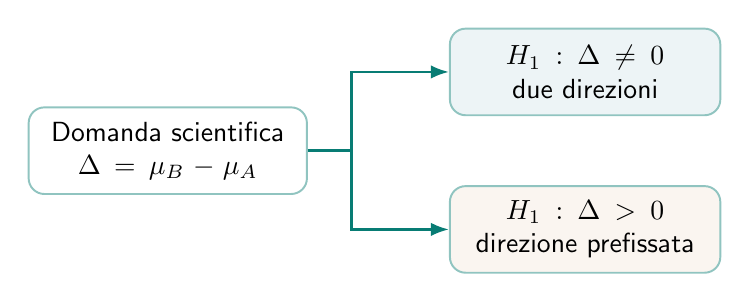
\begin{tikzpicture}[x=1cm,y=1cm]
\node[pFlow,text width=3.3cm] (q) at(1.9,2.0){Domanda scientifica\\$\Delta=\mu_B-\mu_A$};
\node[pFlow,text width=3.2cm,fill=GeoA!8] (b) at(7.2,3.0){$H_1:\Delta\ne0$\\due direzioni};
\node[pFlow,text width=3.2cm,fill=GeoB!8] (u) at(7.2,1.0){$H_1:\Delta>0$\\direzione prefissata};
\draw[pEdge](q.east)--++(.55,0)|-(b.west);
\draw[pEdge](q.east)--++(.55,0)|-(u.west);
\end{tikzpicture}
\[
p_{\mathrm{due}}=2\Pr(T\leq-|t_{\mathrm{obs}}|),\qquad
p_{\mathrm{destra}}=\Pr(T\geq t_{\mathrm{obs}}).
\]
\PSmall{Formule per un riferimento continuo simmetrico. Per un’alternativa a destra, un effetto osservato negativo non è evidenza nella direzione prevista.}

\end{minipage}% 
\end{lrbox}
\typeout{FULLBOX:022:L:\the\ht\PilotLeftBox:\the\dp\PilotLeftBox}
\begin{lrbox}{\PilotRightBox}%
\begin{minipage}[t]{7.55cm}\raggedright\color{Ink}\fontsize{11.3}{14.8}\selectfont

\PCode{R · alternativa dichiarata}{022_direzione.R}
\PBody{Per $t_{\mathrm{obs}}=2$ e $\nu=20$, la coda destra vale circa $0{,}0296$. Il valore bilaterale è circa $0{,}0593$.}
\PInfo{Scegliere la direzione dopo aver visto il segno cambia la procedura. La calibrazione del test deve tenere conto di tale scelta.}

\end{minipage}% 
\end{lrbox}
\typeout{FULLBOX:022:R:\the\ht\PilotRightBox:\the\dp\PilotRightBox}
\begin{frame}[plain]\hypertarget{slide22}{}
\bookmark[level=1,page=22]{Scegliere prima la direzione}
\begin{tikzpicture}[remember picture,overlay]
\PilotChrome{Scegliere prima la direzione}{II · INTERPRETARE L’EVIDENZA}{22}{La direzione dell’alternativa deriva dalla domanda e si definisce prima di osservare il risultato.}
\node[anchor=north west,inner sep=0] at ([xshift=0.96cm,yshift=-2.13cm]current page.north west) {\usebox{\PilotLeftBox}};
\node[anchor=north west,inner sep=0] at ([xshift=11.52cm,yshift=-2.13cm]current page.north west) {\usebox{\PilotRightBox}};

\end{tikzpicture}\end{frame}

% SLIDE 023 | Le probabilità condizionate hanno un verso
\begin{lrbox}{\PilotLeftBox}%
\begin{minipage}[t]{10.05cm}\raggedright\color{Ink}\fontsize{11.3}{14.8}\selectfont

\PLabel{Quale quantità è nota e quale è calcolata?}
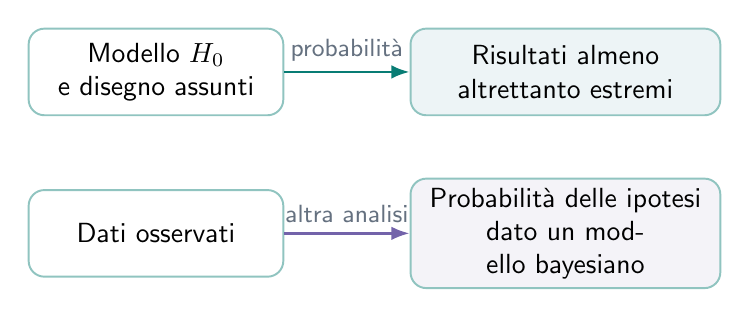
\begin{tikzpicture}[x=1cm,y=1cm]
\node[pFlow,text width=3.0cm] (h) at(1.8,3.1){Modello $H_0$\\e disegno assunti};
\node[pFlow,text width=3.7cm,fill=GeoA!8] (d) at(7.0,3.1){Risultati almeno\\altrettanto estremi};
\draw[pEdge](h)--node[pNote,above]{probabilità}(d);
\node[pFlow,text width=3.0cm] (obs) at(1.8,1.05){Dati osservati};
\node[pFlow,text width=3.7cm,fill=GeoC!8] (post) at(7.0,1.05){Probabilità delle ipotesi\\dato un modello bayesiano};
\draw[pEdge,draw=GeoC](obs)--node[pNote,above]{altra analisi}(post);
\end{tikzpicture}
\[
\Pr(\text{estremità}\mid H_0)\ne\Pr(H_0\mid\text{dati}).
\]

\end{minipage}% 
\end{lrbox}
\typeout{FULLBOX:023:L:\the\ht\PilotLeftBox:\the\dp\PilotLeftBox}
\begin{lrbox}{\PilotRightBox}%
\begin{minipage}[t]{7.55cm}\raggedright\color{Ink}\fontsize{11.3}{14.8}\selectfont

\PLabel{Un’interpretazione corretta}
\PBody{«Se il modello nullo e le ipotesi del test valgono, una statistica almeno altrettanto estrema ha probabilità $p$.»}
\vspace{2mm}
\PLabel{Due conclusioni da correggere}
\PSmall{«$p=0{,}03$: l’ipotesi nulla ha probabilità $3\%$.»\\
«$p=0{,}03$: il risultato è dovuto al caso con probabilità $3\%$.»}
\PInfo{Il p-value non assegna probabilità alle ipotesi e non misura la quota di effetto attribuibile al caso.}

\end{minipage}% 
\end{lrbox}
\typeout{FULLBOX:023:R:\the\ht\PilotRightBox:\the\dp\PilotRightBox}
\begin{frame}[plain]\hypertarget{slide23}{}
\bookmark[level=1,page=23]{Le probabilità condizionate hanno un verso}
\begin{tikzpicture}[remember picture,overlay]
\PilotChrome{Le probabilità condizionate hanno un verso}{II · INTERPRETARE L’EVIDENZA}{23}{Condizionare su un’ipotesi e assegnare una probabilità a quell’ipotesi sono operazioni differenti.}
\node[anchor=north west,inner sep=0] at ([xshift=0.96cm,yshift=-2.13cm]current page.north west) {\usebox{\PilotLeftBox}};
\node[anchor=north west,inner sep=0] at ([xshift=11.52cm,yshift=-2.13cm]current page.north west) {\usebox{\PilotRightBox}};

\end{tikzpicture}\end{frame}

% SLIDE 024 | Due valori vicini alla soglia
\begin{lrbox}{\PilotLeftBox}%
\begin{minipage}[t]{10.05cm}\raggedright\color{Ink}\fontsize{11.3}{14.8}\selectfont

\PLabel{La decisione cambia al confine; l’evidenza è vicina}
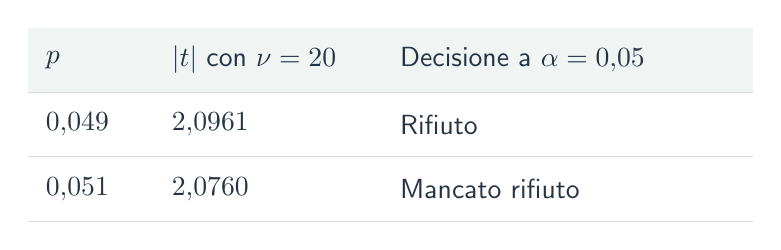
\begin{tikzpicture}[x=1cm,y=1cm]
\fill[GeoTint](0,0)rectangle(9.2,0.82);
\node[pLabel,anchor=west] at(0.1,0.41){$p$};
\node[pLabel,anchor=west] at(1.7000000000000002,0.41){$|t|$ con $\nu=20$};
\node[pLabel,anchor=west] at(4.6,0.41){Decisione a $\alpha=0{,}05$};
\draw[Rule](0,0.0)--(9.2,0.0);
\node[pLabel,anchor=west] at(0.1,-0.41){$0{,}049$};
\node[pLabel,anchor=west] at(1.7000000000000002,-0.41){$2{,}0961$};
\node[pLabel,anchor=west] at(4.6,-0.41){Rifiuto};
\draw[Rule](0,-0.82)--(9.2,-0.82);
\node[pLabel,anchor=west] at(0.1,-1.23){$0{,}051$};
\node[pLabel,anchor=west] at(1.7000000000000002,-1.23){$2{,}0760$};
\node[pLabel,anchor=west] at(4.6,-1.23){Mancato rifiuto};
\draw[Rule](0,-1.64)--(9.2,-1.64);
\end{tikzpicture}
\vspace{3mm}
\PBody{La regola di decisione è discreta. La distanza fra i due p-value rimane piccola e non giustifica descrizioni scientifiche opposte.}
\[
\text{riportare:}\quad\widehat\Delta,\quad IC,\quad p,\quad n,\quad\text{metodo}.
\]

\end{minipage}% 
\end{lrbox}
\typeout{FULLBOX:024:L:\the\ht\PilotLeftBox:\the\dp\PilotLeftBox}
\begin{lrbox}{\PilotRightBox}%
\begin{minipage}[t]{7.55cm}\raggedright\color{Ink}\fontsize{11.3}{14.8}\selectfont

\PCode{R · due punti attorno al confine}{024_soglie_vicine.R}
\PBody{\texttt{qt()} inverte la funzione di ripartizione. Ricostruisce qui le statistiche bilaterali corrispondenti ai due p-value.}
\PInfo{Usare «significativo» e «non significativo» come descrizioni complete nasconde l’entità dell’effetto e la precisione.}

\end{minipage}% 
\end{lrbox}
\typeout{FULLBOX:024:R:\the\ht\PilotRightBox:\the\dp\PilotRightBox}
\begin{frame}[plain]\hypertarget{slide24}{}
\bookmark[level=1,page=24]{Due valori vicini alla soglia}
\begin{tikzpicture}[remember picture,overlay]
\PilotChrome{Due valori vicini alla soglia}{II · INTERPRETARE L’EVIDENZA}{24}{Una soglia rende operativa una decisione; il resoconto conserva stima, intervallo e valore numerico del p-value.}
\node[anchor=north west,inner sep=0] at ([xshift=0.96cm,yshift=-2.13cm]current page.north west) {\usebox{\PilotLeftBox}};
\node[anchor=north west,inner sep=0] at ([xshift=11.52cm,yshift=-2.13cm]current page.north west) {\usebox{\PilotRightBox}};

\end{tikzpicture}\end{frame}

% SLIDE 025 | Effetto e precisione sono due informazioni
\begin{lrbox}{\PilotLeftBox}%
\begin{minipage}[t]{10.05cm}\raggedright\color{Ink}\fontsize{11.3}{14.8}\selectfont

\PLabel{Quattro intervalli costruiti per illustrare la lettura}
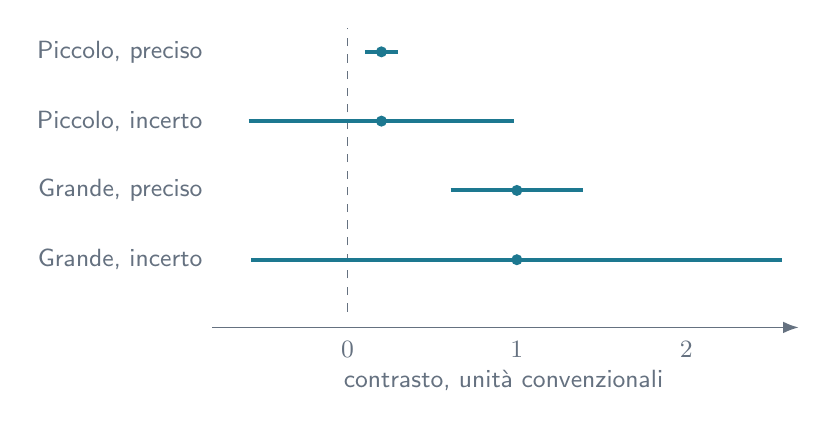
\begin{tikzpicture}[x=1cm,y=1cm]
\draw[Muted,dashed](3.7199999999999998,.1)--(3.7199999999999998,3.7);
\node[pNote,anchor=east] at(2.0,3.4){Piccolo, preciso};
\draw[GeoA,line width=1.4pt](3.9393000000000002,3.4)--(4.3607,3.4);
\fill[GeoA](4.15,3.4)circle(2pt);
\node[pNote,anchor=east] at(2.0,2.52){Piccolo, incerto};
\draw[GeoA,line width=1.4pt](2.4644,2.52)--(5.8355999999999995,2.52);
\fill[GeoA](4.15,2.52)circle(2pt);
\node[pNote,anchor=east] at(2.0,1.64){Grande, preciso};
\draw[GeoA,line width=1.4pt](5.0272,1.64)--(6.7128000000000005,1.64);
\fill[GeoA](5.87,1.64)circle(2pt);
\node[pNote,anchor=east] at(2.0,0.7599999999999998){Grande, incerto};
\draw[GeoA,line width=1.4pt](2.4988,0.7599999999999998)--(9.2412,0.7599999999999998);
\fill[GeoA](5.87,0.7599999999999998)circle(2pt);
\draw[pAxis](2,-.1)--(9.45,-.1);
\node[pNote,below] at(3.7199999999999998,-.15){$ 0 $};
\node[pNote,below] at(5.87,-.15){$ 1 $};
\node[pNote,below] at(8.02,-.15){$ 2 $};
\node[pNote] at(5.7,-.77){contrasto, unità convenzionali};
\end{tikzpicture}
\PSmall{Punti: stime. Segmenti: $\widehat\Delta\pm1{,}96\,SE$. Sono esempi didattici, senza dati osservati sottostanti. «Piccolo» e «grande» richiedono un contesto scientifico.}

\end{minipage}% 
\end{lrbox}
\typeout{FULLBOX:025:L:\the\ht\PilotLeftBox:\the\dp\PilotLeftBox}
\begin{lrbox}{\PilotRightBox}%
\begin{minipage}[t]{7.55cm}\raggedright\color{Ink}\fontsize{11.3}{14.8}\selectfont

\PCode{R · cambiare stima e incertezza}{025_effetto_precisione.R}
\PBody{Un effetto vicino a zero può essere stimato con grande precisione. Un effetto numericamente ampio può avere un intervallo molto largo.}
\PInfo{La precisione riguarda l’incertezza della stima. La rilevanza riguarda le conseguenze scientifiche della differenza.}

\end{minipage}% 
\end{lrbox}
\typeout{FULLBOX:025:R:\the\ht\PilotRightBox:\the\dp\PilotRightBox}
\begin{frame}[plain]\hypertarget{slide25}{}
\bookmark[level=1,page=25]{Effetto e precisione sono due informazioni}
\begin{tikzpicture}[remember picture,overlay]
\PilotChrome{Effetto e precisione sono due informazioni}{II · INTERPRETARE L’EVIDENZA}{25}{Leggere insieme posizione e ampiezza dell’intervallo permette di distinguere entità dell’effetto e incertezza.}
\node[anchor=north west,inner sep=0] at ([xshift=0.96cm,yshift=-2.13cm]current page.north west) {\usebox{\PilotLeftBox}};
\node[anchor=north west,inner sep=0] at ([xshift=11.52cm,yshift=-2.13cm]current page.north west) {\usebox{\PilotRightBox}};

\end{tikzpicture}\end{frame}

% SLIDE 026 | La rilevanza richiede un criterio scientifico
\begin{lrbox}{\PilotLeftBox}%
\begin{minipage}[t]{10.05cm}\raggedright\color{Ink}\fontsize{11.3}{14.8}\selectfont

\PLabel{Una differenza minima da motivare nel problema}
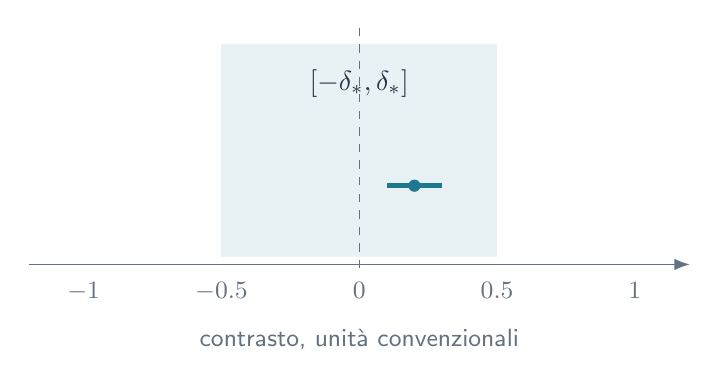
\begin{tikzpicture}[x=1cm,y=1cm]
\fill[GeoA!10](3.25,.4)rectangle(6.75,3.1);
\draw[Muted,dashed](5,.25)--(5,3.3);
\draw[pAxis](.8,.3)--(9.2,.3);
\foreach \x/\v in {1.5/-1,3.25/-0.5,5/0,6.75/0.5,8.5/1}{\node[pNote,below] at(\x,.2){$\v$};}
\draw[GeoA,line width=1.6pt](5.35,1.3)--(6.05,1.3);
\fill[GeoA](5.7,1.3)circle(2.2pt);
\node[pLabel] at(5,2.6){$[-\delta_*,\delta_*]$};
\node[pNote] at(5,-.65){contrasto, unità convenzionali};
\end{tikzpicture}
\PBody{Esempio: $\delta_*=0{,}5$ e intervallo $[0{,}10;0{,}30]$. Lo zero è escluso, ma l’intero intervallo rimane entro il margine scientifico dichiarato.}

\end{minipage}% 
\end{lrbox}
\typeout{FULLBOX:026:L:\the\ht\PilotLeftBox:\the\dp\PilotLeftBox}
\begin{lrbox}{\PilotRightBox}%
\begin{minipage}[t]{7.55cm}\raggedright\color{Ink}\fontsize{11.3}{14.8}\selectfont

\PCode{R · collocare un intervallo}{026_margine_scientifico.R}
\PSmall{Il margine deriva dal problema scientifico e ha le stesse unità di $\Delta$.}
\PInfo{Questo controllo descrive la posizione dell’intervallo. L’equivalenza richiede una procedura inferenziale specifica.}

\end{minipage}% 
\end{lrbox}
\typeout{FULLBOX:026:R:\the\ht\PilotRightBox:\the\dp\PilotRightBox}
\begin{frame}[plain]\hypertarget{slide26}{}
\bookmark[level=1,page=26]{La rilevanza richiede un criterio scientifico}
\begin{tikzpicture}[remember picture,overlay]
\PilotChrome{La rilevanza richiede un criterio scientifico}{II · INTERPRETARE L’EVIDENZA}{26}{Il criterio di rilevanza si definisce con conoscenze del problema; un p-value piccolo non ne stabilisce l’entità.}
\node[anchor=north west,inner sep=0] at ([xshift=0.96cm,yshift=-2.13cm]current page.north west) {\usebox{\PilotLeftBox}};
\node[anchor=north west,inner sep=0] at ([xshift=11.52cm,yshift=-2.13cm]current page.north west) {\usebox{\PilotRightBox}};

\end{tikzpicture}\end{frame}

% SLIDE 027 | Un mancato rifiuto conserva più possibilità
\begin{lrbox}{\PilotLeftBox}%
\begin{minipage}[t]{10.05cm}\raggedright\color{Ink}\fontsize{11.3}{14.8}\selectfont

\PLabel{Intervalli diversi possono entrambi contenere zero}
\begin{tikzpicture}[x=1cm,y=1cm]
\fill[GeoA!10](3.75,.1)rectangle(6.25,3.6);
\draw[Muted,dashed](5,.05)--(5,3.6);
\draw[GeoA,line width=1.6pt](4.4,2.7)--(5.6,2.7);
\fill[GeoA](5,2.7)circle(2pt);
\node[pNote,anchor=east] at(3.3,2.7){stima precisa};
\draw[GeoB,line width=1.6pt](1.3,1.4)--(8.7,1.4);
\fill[GeoB](5,1.4)circle(2pt);
\node[pNote,anchor=west] at(1.3,.75){stima poco precisa};
\draw[pAxis](.8,0)--(9.2,0);
\node[pNote,below] at(3.75,-.1){$-\delta_*$};
\node[pNote,below] at(5,-.1){$0$};
\node[pNote,below] at(6.25,-.1){$\delta_*$};
\end{tikzpicture}
\PBody{Un intervallo ampio può comprendere sia differenze trascurabili sia differenze scientificamente importanti.}

\end{minipage}% 
\end{lrbox}
\typeout{FULLBOX:027:L:\the\ht\PilotLeftBox:\the\dp\PilotLeftBox}
\begin{lrbox}{\PilotRightBox}%
\begin{minipage}[t]{7.55cm}\raggedright\color{Ink}\fontsize{11.3}{14.8}\selectfont

\PLabel{Formulazioni utili}
\PBody{«I dati non consentono di escludere differenze comprese fra questi limiti.»}
\vspace{2mm}
\PBody{«La stima è vicina a zero, ma l’incertezza è ampia rispetto al margine di interesse.»}
\PInfo{Per sostenere l’equivalenza occorre mostrare, con una procedura appropriata e margini prefissati, che le differenze incompatibili con l’equivalenza sono escluse.}

\end{minipage}% 
\end{lrbox}
\typeout{FULLBOX:027:R:\the\ht\PilotRightBox:\the\dp\PilotRightBox}
\begin{frame}[plain]\hypertarget{slide27}{}
\bookmark[level=1,page=27]{Un mancato rifiuto conserva più possibilità}
\begin{tikzpicture}[remember picture,overlay]
\PilotChrome{Un mancato rifiuto conserva più possibilità}{II · INTERPRETARE L’EVIDENZA}{27}{Non rifiutare una differenza nulla non dimostra uguaglianza, assenza di effetto o equivalenza scientifica.}
\node[anchor=north west,inner sep=0] at ([xshift=0.96cm,yshift=-2.13cm]current page.north west) {\usebox{\PilotLeftBox}};
\node[anchor=north west,inner sep=0] at ([xshift=11.52cm,yshift=-2.13cm]current page.north west) {\usebox{\PilotRightBox}};

\end{tikzpicture}\end{frame}

% SLIDE 028 | Gli errori si definiscono nelle ripetizioni
\begin{lrbox}{\PilotLeftBox}%
\begin{minipage}[t]{10.05cm}\raggedright\color{Ink}\fontsize{11.3}{14.8}\selectfont

\PLabel{Stato della popolazione e decisione della procedura}
\begin{tikzpicture}[x=1cm,y=1cm]
\fill[GeoTint](0,0)rectangle(9.35,0.95);
\node[pLabel,anchor=west] at(0.1,0.475){Decisione};
\node[pLabel,anchor=west] at(2.6,0.475){$H_0$ vera};
\node[pLabel,anchor=west] at(5.8,0.475){$H_0$ falsa};
\draw[Rule](0,0.0)--(9.35,0.0);
\node[pLabel,anchor=west] at(0.1,-0.475){Rifiutare $H_0$};
\node[pLabel,anchor=west] at(2.6,-0.475){Errore di I tipo};
\node[pLabel,anchor=west] at(5.8,-0.475){Rifiuto corretto};
\draw[Rule](0,-0.95)--(9.35,-0.95);
\node[pLabel,anchor=west] at(0.1,-1.4249999999999998){Non rifiutare};
\node[pLabel,anchor=west] at(2.6,-1.4249999999999998){Mancato rifiuto\\corretto};
\node[pLabel,anchor=west] at(5.8,-1.4249999999999998){Errore di II tipo};
\draw[Rule](0,-1.9)--(9.35,-1.9);
\end{tikzpicture}
\[
\Pr_{H_0}(\text{rifiuto})\leq\alpha,
\qquad\operatorname{Potenza}(\Delta)=1-\beta(\Delta).
\]
\PSmall{La seconda probabilità dipende dall’alternativa vera, dalla variabilità, dalla numerosità e dal disegno.}

\end{minipage}% 
\end{lrbox}
\typeout{FULLBOX:028:L:\the\ht\PilotLeftBox:\the\dp\PilotLeftBox}
\begin{lrbox}{\PilotRightBox}%
\begin{minipage}[t]{7.55cm}\raggedright\color{Ink}\fontsize{11.3}{14.8}\selectfont

\PLabel{Che cosa controlla il livello?}
\PBody{Con $\alpha=0{,}05$, una procedura valida rifiuta al massimo nel $5\%$ delle ripetizioni compatibili con $H_0$, alle condizioni dichiarate.}
\PInfo{Il livello non è la probabilità che la singola conclusione riportata sia errata. Anche una decisione corretta deve essere accompagnata dalla stima dell’effetto.}

\end{minipage}% 
\end{lrbox}
\typeout{FULLBOX:028:R:\the\ht\PilotRightBox:\the\dp\PilotRightBox}
\begin{frame}[plain]\hypertarget{slide28}{}
\bookmark[level=1,page=28]{Gli errori si definiscono nelle ripetizioni}
\begin{tikzpicture}[remember picture,overlay]
\PilotChrome{Gli errori si definiscono nelle ripetizioni}{II · INTERPRETARE L’EVIDENZA}{28}{Livello e potenza descrivono le prestazioni della procedura su campioni ripetuti, con stati della popolazione specificati.}
\node[anchor=north west,inner sep=0] at ([xshift=0.96cm,yshift=-2.13cm]current page.north west) {\usebox{\PilotLeftBox}};
\node[anchor=north west,inner sep=0] at ([xshift=11.52cm,yshift=-2.13cm]current page.north west) {\usebox{\PilotRightBox}};

\end{tikzpicture}\end{frame}

% SLIDE 029 | Un p-value valido è calibrato sotto $H_0$
\begin{lrbox}{\PilotLeftBox}%
\begin{minipage}[t]{10.05cm}\raggedright\color{Ink}\fontsize{11.3}{14.8}\selectfont

\PLabel{Un riferimento continuo esatto produce p uniformi}
\begin{tikzpicture}[x=1cm,y=1cm]
\draw[Rule](.75,0.0000)--(8.75,0.0000);
\node[pNote,anchor=east] at(.60,0.0000){$ 0 $};
\draw[Rule](.75,1.3250)--(8.75,1.3250);
\node[pNote,anchor=east] at(.60,1.3250){$ 0.5 $};
\draw[Rule](.75,2.6500)--(8.75,2.6500);
\node[pNote,anchor=east] at(.60,2.6500){$ 1 $};
\draw[pAxis](.75,0)--(8.98,0);
\draw[pAxis](.75,0)--(.75,2.81);
\draw[Muted](0.7500,0)--(0.7500,-.07);
\node[pNote,below] at(0.7500,-.08){$ 0 $};
\draw[Muted](2.7500,0)--(2.7500,-.07);
\node[pNote,below] at(2.7500,-.08){$ 0.25 $};
\draw[Muted](4.7500,0)--(4.7500,-.07);
\node[pNote,below] at(4.7500,-.08){$ 0.5 $};
\draw[Muted](6.7500,0)--(6.7500,-.07);
\node[pNote,below] at(6.7500,-.08){$ 0.75 $};
\draw[Muted](8.7500,0)--(8.7500,-.07);
\node[pNote,below] at(8.7500,-.08){$ 1 $};
\node[pNote] at(4.75,-.61){soglia $u$};
\node[pNote,rotate=90] at(-.18,1.325){frequenza $p\leq u$};
\draw[GeoC,dashed,line width=1pt](0.75,0)--(8.75,2.65);
\draw[GeoA,line width=1.1pt,] plot coordinates{(0.75000,0.00000) (0.83000,0.02756) (0.91000,0.05406) (0.99000,0.08162) (1.07000,0.10759) (1.15000,0.13939) (1.23000,0.16271) (1.31000,0.18497) (1.39000,0.20564) (1.47000,0.23002) (1.55000,0.25440) (1.63000,0.27825) (1.71000,0.30369) (1.79000,0.32436) (1.87000,0.34874) (1.95000,0.37365) (2.03000,0.40757) (2.11000,0.43142) (2.19000,0.45898) (2.27000,0.48336) (2.35000,0.51304) (2.43000,0.53477) (2.51000,0.55597) (2.59000,0.58141) (2.67000,0.60791) (2.75000,0.63441) (2.83000,0.65614) (2.91000,0.68476) (2.99000,0.71285) (3.07000,0.73458) (3.15000,0.75790) (3.23000,0.78970) (3.31000,0.81090) (3.39000,0.83846) (3.47000,0.86920) (3.55000,0.89623) (3.63000,0.92008) (3.71000,0.95241) (3.79000,0.98368) (3.87000,1.01124) (3.95000,1.03986) (4.03000,1.06901) (4.11000,1.10081) (4.19000,1.12678) (4.27000,1.15699) (4.35000,1.18402) (4.43000,1.20840) (4.51000,1.23702) (4.59000,1.26246) (4.67000,1.28419) (4.75000,1.31864) (4.83000,1.34037) (4.91000,1.36475) (4.99000,1.40079) (5.07000,1.42888) (5.15000,1.45591) (5.23000,1.48294) (5.31000,1.50096) (5.39000,1.52746) (5.47000,1.56456) (5.55000,1.58894) (5.63000,1.61703) (5.71000,1.64247) (5.79000,1.66950) (5.87000,1.70077) (5.95000,1.72621) (6.03000,1.75695) (6.11000,1.78080) (6.19000,1.81366) (6.27000,1.84228) (6.35000,1.86772) (6.43000,1.89687) (6.51000,1.92390) (6.59000,1.95093) (6.67000,1.98008) (6.75000,2.00923) (6.83000,2.03467) (6.91000,2.06011) (6.99000,2.09350) (7.07000,2.12689) (7.15000,2.16081) (7.23000,2.18572) (7.31000,2.21116) (7.39000,2.23342) (7.47000,2.25303) (7.55000,2.27529) (7.63000,2.30338) (7.71000,2.32988) (7.79000,2.35002) (7.87000,2.37652) (7.95000,2.39878) (8.03000,2.42422) (8.11000,2.45178) (8.19000,2.47828) (8.27000,2.50637) (8.35000,2.52969) (8.43000,2.56255) (8.51000,2.58640) (8.59000,2.60707) (8.67000,2.62562) (8.75000,2.65000)};
\node[pNote,text=GeoA] at(6.6,.6){5\,000 campioni};
\end{tikzpicture}
\[
\Pr_{H_0}(p\leq u)\leq u,\qquad 0\leq u\leq1.
\]
\PSmall{Nel caso continuo esatto vale l’uguaglianza. Con statistiche discrete il test può essere conservativo. La curva empirica oscilla attorno alla diagonale.}

\end{minipage}% 
\end{lrbox}
\typeout{FULLBOX:029:L:\the\ht\PilotLeftBox:\the\dp\PilotLeftBox}
\begin{lrbox}{\PilotRightBox}%
\begin{minipage}[t]{7.55cm}\raggedright\color{Ink}\fontsize{11.3}{14.8}\selectfont

\PCode{R · ripetere un riferimento nullo}{029_calibrazione.R}
\PBody{Qui ogni $Z$ simulato rappresenta una statistica sotto $H_0$. Il modello normale noto rende il p-value continuo ed esatto.}
\PInfo{Una verifica di calibrazione riguarda il procedimento completo, comprese selezioni del modello, filtri e regole di arresto.}

\end{minipage}% 
\end{lrbox}
\typeout{FULLBOX:029:R:\the\ht\PilotRightBox:\the\dp\PilotRightBox}
\begin{frame}[plain]\hypertarget{slide29}{}
\bookmark[level=1,page=29]{Un p-value valido è calibrato sotto $H_0$}
\begin{tikzpicture}[remember picture,overlay]
\PilotChrome{Un p-value valido è calibrato sotto $H_0$}{II · INTERPRETARE L’EVIDENZA}{29}{La calibrazione confronta la frequenza dei p-value piccoli sotto $H_0$ con la soglia usata per decidere.}
\node[anchor=north west,inner sep=0] at ([xshift=0.96cm,yshift=-2.13cm]current page.north west) {\usebox{\PilotLeftBox}};
\node[anchor=north west,inner sep=0] at ([xshift=11.52cm,yshift=-2.13cm]current page.north west) {\usebox{\PilotRightBox}};

\end{tikzpicture}\end{frame}

% SLIDE 030 | La potenza dipende dall’effetto vero
\begin{lrbox}{\PilotLeftBox}%
\begin{minipage}[t]{10.05cm}\raggedright\color{Ink}\fontsize{11.3}{14.8}\selectfont

\PLabel{Esempio normale: varianze note e due gruppi indipendenti}
\begin{tikzpicture}[x=1cm,y=1cm]
\draw[Rule](.75,0.0000)--(8.75,0.0000);
\node[pNote,anchor=east] at(.60,0.0000){$ 0 $};
\draw[Rule](.75,1.1905)--(8.75,1.1905);
\node[pNote,anchor=east] at(.60,1.1905){$ 0.2 $};
\draw[Rule](.75,2.3810)--(8.75,2.3810);
\node[pNote,anchor=east] at(.60,2.3810){$ 0.4 $};
\draw[pAxis](.75,0)--(8.98,0);
\draw[pAxis](.75,0)--(.75,2.66);
\draw[Muted](2.0833,0)--(2.0833,-.07);
\node[pNote,below] at(2.0833,-.08){$ -4 $};
\draw[Muted](3.4167,0)--(3.4167,-.07);
\node[pNote,below] at(3.4167,-.08){$ -2 $};
\draw[Muted](4.7500,0)--(4.7500,-.07);
\node[pNote,below] at(4.7500,-.08){$ 0 $};
\draw[Muted](6.0833,0)--(6.0833,-.07);
\node[pNote,below] at(6.0833,-.08){$ 2 $};
\draw[Muted](7.4167,0)--(7.4167,-.07);
\node[pNote,below] at(7.4167,-.08){$ 4 $};
\node[pNote] at(4.75,-.61){statistica $Z$};
\node[pNote,rotate=90] at(-.18,1.25){densità};
\fill[GeoB!45] (0.75000,0)-- plot coordinates{(0.75000,0.00000) (0.76333,0.00000) (0.77667,0.00000) (0.79000,0.00000) (0.80333,0.00000) (0.81667,0.00000) (0.83000,0.00000) (0.84333,0.00000) (0.85667,0.00000) (0.87000,0.00000) (0.88333,0.00000) (0.89667,0.00000) (0.91000,0.00000) (0.92333,0.00000) (0.93667,0.00000) (0.95000,0.00000) (0.96333,0.00000) (0.97667,0.00000) (0.99000,0.00000) (1.00333,0.00000) (1.01667,0.00000) (1.03000,0.00000) (1.04333,0.00000) (1.05667,0.00000) (1.07000,0.00000) (1.08333,0.00000) (1.09667,0.00000) (1.11000,0.00000) (1.12333,0.00000) (1.13667,0.00000) (1.15000,0.00000) (1.16333,0.00000) (1.17667,0.00000) (1.19000,0.00000) (1.20333,0.00000) (1.21667,0.00000) (1.23000,0.00000) (1.24333,0.00000) (1.25667,0.00000) (1.27000,0.00000) (1.28333,0.00000) (1.29667,0.00000) (1.31000,0.00000) (1.32333,0.00000) (1.33667,0.00000) (1.35000,0.00000) (1.36333,0.00000) (1.37667,0.00000) (1.39000,0.00000) (1.40333,0.00000) (1.41667,0.00000) (1.43000,0.00000) (1.44333,0.00000) (1.45667,0.00000) (1.47000,0.00000) (1.48333,0.00000) (1.49667,0.00000) (1.51000,0.00000) (1.52333,0.00000) (1.53667,0.00000) (1.55000,0.00000) (1.56333,0.00000) (1.57667,0.00000) (1.59000,0.00000) (1.60333,0.00000) (1.61667,0.00000) (1.63000,0.00000) (1.64333,0.00000) (1.65667,0.00000) (1.67000,0.00000) (1.68333,0.00000) (1.69667,0.00000) (1.71000,0.00000) (1.72333,0.00000) (1.73667,0.00000) (1.75000,0.00000) (1.76333,0.00000) (1.77667,0.00000) (1.79000,0.00000) (1.80333,0.00000) (1.81667,0.00000) (1.83000,0.00000) (1.84333,0.00000) (1.85667,0.00000) (1.87000,0.00000) (1.88333,0.00000) (1.89667,0.00000) (1.91000,0.00000) (1.92333,0.00000) (1.93667,0.00000) (1.95000,0.00000) (1.96333,0.00000) (1.97667,0.00000) (1.99000,0.00000) (2.00333,0.00000) (2.01667,0.00000) (2.03000,0.00000) (2.04333,0.00000) (2.05667,0.00000) (2.07000,0.00000) (2.08333,0.00000) (2.09667,0.00000) (2.11000,0.00000) (2.12333,0.00000) (2.13667,0.00000) (2.15000,0.00000) (2.16333,0.00000) (2.17667,0.00000) (2.19000,0.00000) (2.20333,0.00000) (2.21667,0.00000) (2.23000,0.00000) (2.24333,0.00000) (2.25667,0.00000) (2.27000,0.00000) (2.28333,0.00000) (2.29667,0.00000) (2.31000,0.00000) (2.32333,0.00000) (2.33667,0.00000) (2.35000,0.00000) (2.36333,0.00000) (2.37667,0.00000) (2.39000,0.00000) (2.40333,0.00000) (2.41667,0.00000) (2.43000,0.00000) (2.44333,0.00000) (2.45667,0.00000) (2.47000,0.00000) (2.48333,0.00000) (2.49667,0.00000) (2.51000,0.00000) (2.52333,0.00000) (2.53667,0.00000) (2.55000,0.00000) (2.56333,0.00000) (2.57667,0.00000) (2.59000,0.00000) (2.60333,0.00000) (2.61667,0.00000) (2.63000,0.00000) (2.64333,0.00001) (2.65667,0.00001) (2.67000,0.00001) (2.68333,0.00001) (2.69667,0.00001) (2.71000,0.00001) (2.72333,0.00001) (2.73667,0.00001) (2.75000,0.00001) (2.76333,0.00001) (2.77667,0.00001) (2.79000,0.00002) (2.80333,0.00002) (2.81667,0.00002) (2.83000,0.00002) (2.84333,0.00002) (2.85667,0.00003) (2.87000,0.00003) (2.88333,0.00003) (2.89667,0.00004) (2.91000,0.00004) (2.92333,0.00004) (2.93667,0.00005) (2.95000,0.00005) (2.96333,0.00006) (2.97667,0.00006) (2.99000,0.00007) (3.00333,0.00007) (3.01667,0.00008) (3.03000,0.00009) (3.04333,0.00010) (3.05667,0.00011) (3.07000,0.00012) (3.08333,0.00013) (3.09667,0.00014) (3.11000,0.00015) (3.12333,0.00016) (3.13667,0.00018) (3.15000,0.00020) (3.16333,0.00021) (3.17667,0.00023) (3.19000,0.00025) (3.20333,0.00028) (3.21667,0.00030) (3.23000,0.00033) (3.24333,0.00036) (3.25667,0.00039) (3.27000,0.00042) (3.28333,0.00046) (3.29667,0.00050) (3.31000,0.00054) (3.32333,0.00058) (3.33667,0.00063) (3.35000,0.00069) (3.36333,0.00075) (3.37667,0.00081) (3.39000,0.00087) (3.40333,0.00095) (3.41667,0.00102) (3.43000,0.00111) (3.44333,0.00120)}--(3.44333,0)--cycle;
\fill[GeoB!45] (6.05667,0)-- plot coordinates{(6.05667,2.37400) (6.07000,2.37241) (6.08333,2.36987) (6.09667,2.36639) (6.11000,2.36197) (6.12333,2.35661) (6.13667,2.35033) (6.15000,2.34312) (6.16333,2.33501) (6.17667,2.32599) (6.19000,2.31608) (6.20333,2.30529) (6.21667,2.29363) (6.23000,2.28111) (6.24333,2.26776) (6.25667,2.25359) (6.27000,2.23861) (6.28333,2.22284) (6.29667,2.20629) (6.31000,2.18900) (6.32333,2.17097) (6.33667,2.15223) (6.35000,2.13279) (6.36333,2.11269) (6.37667,2.09194) (6.39000,2.07057) (6.40333,2.04859) (6.41667,2.02604) (6.43000,2.00293) (6.44333,1.97930) (6.45667,1.95516) (6.47000,1.93054) (6.48333,1.90547) (6.49667,1.87998) (6.51000,1.85408) (6.52333,1.82781) (6.53667,1.80120) (6.55000,1.77425) (6.56333,1.74702) (6.57667,1.71951) (6.59000,1.69176) (6.60333,1.66379) (6.61667,1.63563) (6.63000,1.60731) (6.64333,1.57884) (6.65667,1.55025) (6.67000,1.52158) (6.68333,1.49284) (6.69667,1.46405) (6.71000,1.43525) (6.72333,1.40645) (6.73667,1.37768) (6.75000,1.34895) (6.76333,1.32030) (6.77667,1.29174) (6.79000,1.26329) (6.80333,1.23497) (6.81667,1.20681) (6.83000,1.17881) (6.84333,1.15101) (6.85667,1.12341) (6.87000,1.09603) (6.88333,1.06890) (6.89667,1.04201) (6.91000,1.01540) (6.92333,0.98908) (6.93667,0.96305) (6.95000,0.93733) (6.96333,0.91193) (6.97667,0.88686) (6.99000,0.86214) (7.00333,0.83778) (7.01667,0.81377) (7.03000,0.79014) (7.04333,0.76689) (7.05667,0.74402) (7.07000,0.72155) (7.08333,0.69947) (7.09667,0.67780) (7.11000,0.65654) (7.12333,0.63569) (7.13667,0.61526) (7.15000,0.59525) (7.16333,0.57565) (7.17667,0.55648) (7.19000,0.53774) (7.20333,0.51941) (7.21667,0.50151) (7.23000,0.48403) (7.24333,0.46698) (7.25667,0.45035) (7.27000,0.43413) (7.28333,0.41833) (7.29667,0.40295) (7.31000,0.38797) (7.32333,0.37341) (7.33667,0.35924) (7.35000,0.34548) (7.36333,0.33211) (7.37667,0.31913) (7.39000,0.30653) (7.40333,0.29431) (7.41667,0.28247) (7.43000,0.27100) (7.44333,0.25988) (7.45667,0.24913) (7.47000,0.23872) (7.48333,0.22866) (7.49667,0.21893) (7.51000,0.20953) (7.52333,0.20046) (7.53667,0.19170) (7.55000,0.18325) (7.56333,0.17511) (7.57667,0.16726) (7.59000,0.15969) (7.60333,0.15241) (7.61667,0.14540) (7.63000,0.13866) (7.64333,0.13218) (7.65667,0.12595) (7.67000,0.11997) (7.68333,0.11423) (7.69667,0.10871) (7.71000,0.10342) (7.72333,0.09835) (7.73667,0.09349) (7.75000,0.08884) (7.76333,0.08438) (7.77667,0.08012) (7.79000,0.07604) (7.80333,0.07214) (7.81667,0.06841) (7.83000,0.06484) (7.84333,0.06144) (7.85667,0.05820) (7.87000,0.05510) (7.88333,0.05215) (7.89667,0.04934) (7.91000,0.04665) (7.92333,0.04410) (7.93667,0.04167) (7.95000,0.03936) (7.96333,0.03716) (7.97667,0.03507) (7.99000,0.03309) (8.00333,0.03120) (8.01667,0.02941) (8.03000,0.02771) (8.04333,0.02610) (8.05667,0.02458) (8.07000,0.02313) (8.08333,0.02176) (8.09667,0.02046) (8.11000,0.01923) (8.12333,0.01807) (8.13667,0.01698) (8.15000,0.01594) (8.16333,0.01496) (8.17667,0.01403) (8.19000,0.01316) (8.20333,0.01233) (8.21667,0.01156) (8.23000,0.01083) (8.24333,0.01014) (8.25667,0.00949) (8.27000,0.00887) (8.28333,0.00830) (8.29667,0.00776) (8.31000,0.00725) (8.32333,0.00677) (8.33667,0.00632) (8.35000,0.00590) (8.36333,0.00550) (8.37667,0.00513) (8.39000,0.00478) (8.40333,0.00446) (8.41667,0.00415) (8.43000,0.00386) (8.44333,0.00360) (8.45667,0.00335) (8.47000,0.00311) (8.48333,0.00289) (8.49667,0.00269) (8.51000,0.00250) (8.52333,0.00232) (8.53667,0.00215) (8.55000,0.00199) (8.56333,0.00185) (8.57667,0.00171) (8.59000,0.00159) (8.60333,0.00147) (8.61667,0.00136) (8.63000,0.00126) (8.64333,0.00117) (8.65667,0.00108) (8.67000,0.00100) (8.68333,0.00092) (8.69667,0.00085) (8.71000,0.00079) (8.72333,0.00072) (8.73667,0.00067) (8.75000,0.00062)}--(8.75000,0)--cycle;
\draw[GeoA,line width=1.1pt,] plot coordinates{(0.75000,0.00000) (0.76333,0.00000) (0.77667,0.00000) (0.79000,0.00000) (0.80333,0.00000) (0.81667,0.00000) (0.83000,0.00000) (0.84333,0.00000) (0.85667,0.00000) (0.87000,0.00000) (0.88333,0.00000) (0.89667,0.00000) (0.91000,0.00000) (0.92333,0.00000) (0.93667,0.00000) (0.95000,0.00000) (0.96333,0.00000) (0.97667,0.00000) (0.99000,0.00000) (1.00333,0.00000) (1.01667,0.00000) (1.03000,0.00000) (1.04333,0.00000) (1.05667,0.00000) (1.07000,0.00000) (1.08333,0.00000) (1.09667,0.00000) (1.11000,0.00000) (1.12333,0.00000) (1.13667,0.00000) (1.15000,0.00000) (1.16333,0.00000) (1.17667,0.00000) (1.19000,0.00000) (1.20333,0.00000) (1.21667,0.00000) (1.23000,0.00000) (1.24333,0.00000) (1.25667,0.00000) (1.27000,0.00000) (1.28333,0.00000) (1.29667,0.00000) (1.31000,0.00000) (1.32333,0.00000) (1.33667,0.00000) (1.35000,0.00001) (1.36333,0.00001) (1.37667,0.00001) (1.39000,0.00001) (1.40333,0.00001) (1.41667,0.00001) (1.43000,0.00001) (1.44333,0.00001) (1.45667,0.00001) (1.47000,0.00001) (1.48333,0.00001) (1.49667,0.00002) (1.51000,0.00002) (1.52333,0.00002) (1.53667,0.00002) (1.55000,0.00002) (1.56333,0.00003) (1.57667,0.00003) (1.59000,0.00003) (1.60333,0.00003) (1.61667,0.00004) (1.63000,0.00004) (1.64333,0.00005) (1.65667,0.00005) (1.67000,0.00006) (1.68333,0.00006) (1.69667,0.00007) (1.71000,0.00007) (1.72333,0.00008) (1.73667,0.00009) (1.75000,0.00010) (1.76333,0.00010) (1.77667,0.00011) (1.79000,0.00012) (1.80333,0.00014) (1.81667,0.00015) (1.83000,0.00016) (1.84333,0.00018) (1.85667,0.00019) (1.87000,0.00021) (1.88333,0.00023) (1.89667,0.00025) (1.91000,0.00027) (1.92333,0.00030) (1.93667,0.00032) (1.95000,0.00035) (1.96333,0.00038) (1.97667,0.00041) (1.99000,0.00045) (2.00333,0.00049) (2.01667,0.00053) (2.03000,0.00058) (2.04333,0.00063) (2.05667,0.00068) (2.07000,0.00074) (2.08333,0.00080) (2.09667,0.00086) (2.11000,0.00093) (2.12333,0.00101) (2.13667,0.00109) (2.15000,0.00118) (2.16333,0.00128) (2.17667,0.00138) (2.19000,0.00149) (2.20333,0.00161) (2.21667,0.00174) (2.23000,0.00187) (2.24333,0.00202) (2.25667,0.00218) (2.27000,0.00235) (2.28333,0.00253) (2.29667,0.00272) (2.31000,0.00293) (2.32333,0.00315) (2.33667,0.00339) (2.35000,0.00364) (2.36333,0.00391) (2.37667,0.00420) (2.39000,0.00451) (2.40333,0.00484) (2.41667,0.00519) (2.43000,0.00557) (2.44333,0.00597) (2.45667,0.00640) (2.47000,0.00685) (2.48333,0.00733) (2.49667,0.00785) (2.51000,0.00840) (2.52333,0.00898) (2.53667,0.00960) (2.55000,0.01025) (2.56333,0.01095) (2.57667,0.01169) (2.59000,0.01248) (2.60333,0.01331) (2.61667,0.01419) (2.63000,0.01513) (2.64333,0.01612) (2.65667,0.01716) (2.67000,0.01827) (2.68333,0.01945) (2.69667,0.02068) (2.71000,0.02199) (2.72333,0.02338) (2.73667,0.02484) (2.75000,0.02638) (2.76333,0.02801) (2.77667,0.02972) (2.79000,0.03153) (2.80333,0.03343) (2.81667,0.03543) (2.83000,0.03754) (2.84333,0.03976) (2.85667,0.04209) (2.87000,0.04454) (2.88333,0.04712) (2.89667,0.04982) (2.91000,0.05266) (2.92333,0.05563) (2.93667,0.05876) (2.95000,0.06203) (2.96333,0.06546) (2.97667,0.06905) (2.99000,0.07281) (3.00333,0.07674) (3.01667,0.08085) (3.03000,0.08515) (3.04333,0.08964) (3.05667,0.09433) (3.07000,0.09923) (3.08333,0.10434) (3.09667,0.10966) (3.11000,0.11522) (3.12333,0.12100) (3.13667,0.12703) (3.15000,0.13330) (3.16333,0.13983) (3.17667,0.14661) (3.19000,0.15367) (3.20333,0.16100) (3.21667,0.16861) (3.23000,0.17652) (3.24333,0.18471) (3.25667,0.19322) (3.27000,0.20203) (3.28333,0.21116) (3.29667,0.22061) (3.31000,0.23040) (3.32333,0.24052) (3.33667,0.25099) (3.35000,0.26181) (3.36333,0.27298) (3.37667,0.28452) (3.39000,0.29643) (3.40333,0.30871) (3.41667,0.32137) (3.43000,0.33442) (3.44333,0.34786) (3.45667,0.36170) (3.47000,0.37593) (3.48333,0.39057) (3.49667,0.40562) (3.51000,0.42107) (3.52333,0.43695) (3.53667,0.45323) (3.55000,0.46994) (3.56333,0.48707) (3.57667,0.50462) (3.59000,0.52260) (3.60333,0.54099) (3.61667,0.55982) (3.63000,0.57906) (3.64333,0.59873) (3.65667,0.61882) (3.67000,0.63932) (3.68333,0.66024) (3.69667,0.68158) (3.71000,0.70332) (3.72333,0.72546) (3.73667,0.74800) (3.75000,0.77094) (3.76333,0.79426) (3.77667,0.81796) (3.79000,0.84202) (3.80333,0.86645) (3.81667,0.89123) (3.83000,0.91636) (3.84333,0.94181) (3.85667,0.96759) (3.87000,0.99367) (3.88333,1.02005) (3.89667,1.04671) (3.91000,1.07364) (3.92333,1.10082) (3.93667,1.12823) (3.95000,1.15587) (3.96333,1.18371) (3.97667,1.21173) (3.99000,1.23993) (4.00333,1.26827) (4.01667,1.29674) (4.03000,1.32532) (4.04333,1.35399) (4.05667,1.38272) (4.07000,1.41150) (4.08333,1.44030) (4.09667,1.46910) (4.11000,1.49788) (4.12333,1.52661) (4.13667,1.55528) (4.15000,1.58384) (4.16333,1.61229) (4.17667,1.64058) (4.19000,1.66871) (4.20333,1.69664) (4.21667,1.72435) (4.23000,1.75182) (4.24333,1.77900) (4.25667,1.80589) (4.27000,1.83245) (4.28333,1.85865) (4.29667,1.88448) (4.31000,1.90990) (4.32333,1.93489) (4.33667,1.95943) (4.35000,1.98348) (4.36333,2.00702) (4.37667,2.03003) (4.39000,2.05249) (4.40333,2.07436) (4.41667,2.09563) (4.43000,2.11627) (4.44333,2.13625) (4.45667,2.15556) (4.47000,2.17418) (4.48333,2.19208) (4.49667,2.20925) (4.51000,2.22566) (4.52333,2.24129) (4.53667,2.25613) (4.55000,2.27017) (4.56333,2.28337) (4.57667,2.29573) (4.59000,2.30724) (4.60333,2.31788) (4.61667,2.32764) (4.63000,2.33650) (4.64333,2.34445) (4.65667,2.35150) (4.67000,2.35762) (4.68333,2.36281) (4.69667,2.36707) (4.71000,2.37039) (4.72333,2.37276) (4.73667,2.37418) (4.75000,2.37466) (4.76333,2.37418) (4.77667,2.37276) (4.79000,2.37039) (4.80333,2.36707) (4.81667,2.36281) (4.83000,2.35762) (4.84333,2.35150) (4.85667,2.34445) (4.87000,2.33650) (4.88333,2.32764) (4.89667,2.31788) (4.91000,2.30724) (4.92333,2.29573) (4.93667,2.28337) (4.95000,2.27017) (4.96333,2.25613) (4.97667,2.24129) (4.99000,2.22566) (5.00333,2.20925) (5.01667,2.19208) (5.03000,2.17418) (5.04333,2.15556) (5.05667,2.13625) (5.07000,2.11627) (5.08333,2.09563) (5.09667,2.07436) (5.11000,2.05249) (5.12333,2.03003) (5.13667,2.00702) (5.15000,1.98348) (5.16333,1.95943) (5.17667,1.93489) (5.19000,1.90990) (5.20333,1.88448) (5.21667,1.85865) (5.23000,1.83245) (5.24333,1.80589) (5.25667,1.77900) (5.27000,1.75182) (5.28333,1.72435) (5.29667,1.69664) (5.31000,1.66871) (5.32333,1.64058) (5.33667,1.61229) (5.35000,1.58384) (5.36333,1.55528) (5.37667,1.52661) (5.39000,1.49788) (5.40333,1.46910) (5.41667,1.44030) (5.43000,1.41150) (5.44333,1.38272) (5.45667,1.35399) (5.47000,1.32532) (5.48333,1.29674) (5.49667,1.26827) (5.51000,1.23993) (5.52333,1.21173) (5.53667,1.18371) (5.55000,1.15587) (5.56333,1.12823) (5.57667,1.10082) (5.59000,1.07364) (5.60333,1.04671) (5.61667,1.02005) (5.63000,0.99367) (5.64333,0.96759) (5.65667,0.94181) (5.67000,0.91636) (5.68333,0.89123) (5.69667,0.86645) (5.71000,0.84202) (5.72333,0.81796) (5.73667,0.79426) (5.75000,0.77094) (5.76333,0.74800) (5.77667,0.72546) (5.79000,0.70332) (5.80333,0.68158) (5.81667,0.66024) (5.83000,0.63932) (5.84333,0.61882) (5.85667,0.59873) (5.87000,0.57906) (5.88333,0.55982) (5.89667,0.54099) (5.91000,0.52260) (5.92333,0.50462) (5.93667,0.48707) (5.95000,0.46994) (5.96333,0.45323) (5.97667,0.43695) (5.99000,0.42107) (6.00333,0.40562) (6.01667,0.39057) (6.03000,0.37593) (6.04333,0.36170) (6.05667,0.34786) (6.07000,0.33442) (6.08333,0.32137) (6.09667,0.30871) (6.11000,0.29643) (6.12333,0.28452) (6.13667,0.27298) (6.15000,0.26181) (6.16333,0.25099) (6.17667,0.24052) (6.19000,0.23040) (6.20333,0.22061) (6.21667,0.21116) (6.23000,0.20203) (6.24333,0.19322) (6.25667,0.18471) (6.27000,0.17652) (6.28333,0.16861) (6.29667,0.16100) (6.31000,0.15367) (6.32333,0.14661) (6.33667,0.13983) (6.35000,0.13330) (6.36333,0.12703) (6.37667,0.12100) (6.39000,0.11522) (6.40333,0.10966) (6.41667,0.10434) (6.43000,0.09923) (6.44333,0.09433) (6.45667,0.08964) (6.47000,0.08515) (6.48333,0.08085) (6.49667,0.07674) (6.51000,0.07281) (6.52333,0.06905) (6.53667,0.06546) (6.55000,0.06203) (6.56333,0.05876) (6.57667,0.05563) (6.59000,0.05266) (6.60333,0.04982) (6.61667,0.04712) (6.63000,0.04454) (6.64333,0.04209) (6.65667,0.03976) (6.67000,0.03754) (6.68333,0.03543) (6.69667,0.03343) (6.71000,0.03153) (6.72333,0.02972) (6.73667,0.02801) (6.75000,0.02638) (6.76333,0.02484) (6.77667,0.02338) (6.79000,0.02199) (6.80333,0.02068) (6.81667,0.01945) (6.83000,0.01827) (6.84333,0.01716) (6.85667,0.01612) (6.87000,0.01513) (6.88333,0.01419) (6.89667,0.01331) (6.91000,0.01248) (6.92333,0.01169) (6.93667,0.01095) (6.95000,0.01025) (6.96333,0.00960) (6.97667,0.00898) (6.99000,0.00840) (7.00333,0.00785) (7.01667,0.00733) (7.03000,0.00685) (7.04333,0.00640) (7.05667,0.00597) (7.07000,0.00557) (7.08333,0.00519) (7.09667,0.00484) (7.11000,0.00451) (7.12333,0.00420) (7.13667,0.00391) (7.15000,0.00364) (7.16333,0.00339) (7.17667,0.00315) (7.19000,0.00293) (7.20333,0.00272) (7.21667,0.00253) (7.23000,0.00235) (7.24333,0.00218) (7.25667,0.00202) (7.27000,0.00187) (7.28333,0.00174) (7.29667,0.00161) (7.31000,0.00149) (7.32333,0.00138) (7.33667,0.00128) (7.35000,0.00118) (7.36333,0.00109) (7.37667,0.00101) (7.39000,0.00093) (7.40333,0.00086) (7.41667,0.00080) (7.43000,0.00074) (7.44333,0.00068) (7.45667,0.00063) (7.47000,0.00058) (7.48333,0.00053) (7.49667,0.00049) (7.51000,0.00045) (7.52333,0.00041) (7.53667,0.00038) (7.55000,0.00035) (7.56333,0.00032) (7.57667,0.00030) (7.59000,0.00027) (7.60333,0.00025) (7.61667,0.00023) (7.63000,0.00021) (7.64333,0.00019) (7.65667,0.00018) (7.67000,0.00016) (7.68333,0.00015) (7.69667,0.00014) (7.71000,0.00012) (7.72333,0.00011) (7.73667,0.00010) (7.75000,0.00010) (7.76333,0.00009) (7.77667,0.00008) (7.79000,0.00007) (7.80333,0.00007) (7.81667,0.00006) (7.83000,0.00006) (7.84333,0.00005) (7.85667,0.00005) (7.87000,0.00004) (7.88333,0.00004) (7.89667,0.00003) (7.91000,0.00003) (7.92333,0.00003) (7.93667,0.00003) (7.95000,0.00002) (7.96333,0.00002) (7.97667,0.00002) (7.99000,0.00002) (8.00333,0.00002) (8.01667,0.00001) (8.03000,0.00001) (8.04333,0.00001) (8.05667,0.00001) (8.07000,0.00001) (8.08333,0.00001) (8.09667,0.00001) (8.11000,0.00001) (8.12333,0.00001) (8.13667,0.00001) (8.15000,0.00001) (8.16333,0.00000) (8.17667,0.00000) (8.19000,0.00000) (8.20333,0.00000) (8.21667,0.00000) (8.23000,0.00000) (8.24333,0.00000) (8.25667,0.00000) (8.27000,0.00000) (8.28333,0.00000) (8.29667,0.00000) (8.31000,0.00000) (8.32333,0.00000) (8.33667,0.00000) (8.35000,0.00000) (8.36333,0.00000) (8.37667,0.00000) (8.39000,0.00000) (8.40333,0.00000) (8.41667,0.00000) (8.43000,0.00000) (8.44333,0.00000) (8.45667,0.00000) (8.47000,0.00000) (8.48333,0.00000) (8.49667,0.00000) (8.51000,0.00000) (8.52333,0.00000) (8.53667,0.00000) (8.55000,0.00000) (8.56333,0.00000) (8.57667,0.00000) (8.59000,0.00000) (8.60333,0.00000) (8.61667,0.00000) (8.63000,0.00000) (8.64333,0.00000) (8.65667,0.00000) (8.67000,0.00000) (8.68333,0.00000) (8.69667,0.00000) (8.71000,0.00000) (8.72333,0.00000) (8.73667,0.00000) (8.75000,0.00000)};
\draw[GeoB,line width=1.1pt,] plot coordinates{(0.75000,0.00000) (0.76333,0.00000) (0.77667,0.00000) (0.79000,0.00000) (0.80333,0.00000) (0.81667,0.00000) (0.83000,0.00000) (0.84333,0.00000) (0.85667,0.00000) (0.87000,0.00000) (0.88333,0.00000) (0.89667,0.00000) (0.91000,0.00000) (0.92333,0.00000) (0.93667,0.00000) (0.95000,0.00000) (0.96333,0.00000) (0.97667,0.00000) (0.99000,0.00000) (1.00333,0.00000) (1.01667,0.00000) (1.03000,0.00000) (1.04333,0.00000) (1.05667,0.00000) (1.07000,0.00000) (1.08333,0.00000) (1.09667,0.00000) (1.11000,0.00000) (1.12333,0.00000) (1.13667,0.00000) (1.15000,0.00000) (1.16333,0.00000) (1.17667,0.00000) (1.19000,0.00000) (1.20333,0.00000) (1.21667,0.00000) (1.23000,0.00000) (1.24333,0.00000) (1.25667,0.00000) (1.27000,0.00000) (1.28333,0.00000) (1.29667,0.00000) (1.31000,0.00000) (1.32333,0.00000) (1.33667,0.00000) (1.35000,0.00000) (1.36333,0.00000) (1.37667,0.00000) (1.39000,0.00000) (1.40333,0.00000) (1.41667,0.00000) (1.43000,0.00000) (1.44333,0.00000) (1.45667,0.00000) (1.47000,0.00000) (1.48333,0.00000) (1.49667,0.00000) (1.51000,0.00000) (1.52333,0.00000) (1.53667,0.00000) (1.55000,0.00000) (1.56333,0.00000) (1.57667,0.00000) (1.59000,0.00000) (1.60333,0.00000) (1.61667,0.00000) (1.63000,0.00000) (1.64333,0.00000) (1.65667,0.00000) (1.67000,0.00000) (1.68333,0.00000) (1.69667,0.00000) (1.71000,0.00000) (1.72333,0.00000) (1.73667,0.00000) (1.75000,0.00000) (1.76333,0.00000) (1.77667,0.00000) (1.79000,0.00000) (1.80333,0.00000) (1.81667,0.00000) (1.83000,0.00000) (1.84333,0.00000) (1.85667,0.00000) (1.87000,0.00000) (1.88333,0.00000) (1.89667,0.00000) (1.91000,0.00000) (1.92333,0.00000) (1.93667,0.00000) (1.95000,0.00000) (1.96333,0.00000) (1.97667,0.00000) (1.99000,0.00000) (2.00333,0.00000) (2.01667,0.00000) (2.03000,0.00000) (2.04333,0.00000) (2.05667,0.00000) (2.07000,0.00000) (2.08333,0.00000) (2.09667,0.00000) (2.11000,0.00000) (2.12333,0.00000) (2.13667,0.00000) (2.15000,0.00000) (2.16333,0.00000) (2.17667,0.00000) (2.19000,0.00000) (2.20333,0.00000) (2.21667,0.00000) (2.23000,0.00000) (2.24333,0.00000) (2.25667,0.00000) (2.27000,0.00000) (2.28333,0.00000) (2.29667,0.00000) (2.31000,0.00000) (2.32333,0.00000) (2.33667,0.00000) (2.35000,0.00000) (2.36333,0.00000) (2.37667,0.00000) (2.39000,0.00000) (2.40333,0.00000) (2.41667,0.00000) (2.43000,0.00000) (2.44333,0.00000) (2.45667,0.00000) (2.47000,0.00000) (2.48333,0.00000) (2.49667,0.00000) (2.51000,0.00000) (2.52333,0.00000) (2.53667,0.00000) (2.55000,0.00000) (2.56333,0.00000) (2.57667,0.00000) (2.59000,0.00000) (2.60333,0.00000) (2.61667,0.00000) (2.63000,0.00000) (2.64333,0.00001) (2.65667,0.00001) (2.67000,0.00001) (2.68333,0.00001) (2.69667,0.00001) (2.71000,0.00001) (2.72333,0.00001) (2.73667,0.00001) (2.75000,0.00001) (2.76333,0.00001) (2.77667,0.00001) (2.79000,0.00002) (2.80333,0.00002) (2.81667,0.00002) (2.83000,0.00002) (2.84333,0.00002) (2.85667,0.00003) (2.87000,0.00003) (2.88333,0.00003) (2.89667,0.00004) (2.91000,0.00004) (2.92333,0.00004) (2.93667,0.00005) (2.95000,0.00005) (2.96333,0.00006) (2.97667,0.00006) (2.99000,0.00007) (3.00333,0.00007) (3.01667,0.00008) (3.03000,0.00009) (3.04333,0.00010) (3.05667,0.00011) (3.07000,0.00012) (3.08333,0.00013) (3.09667,0.00014) (3.11000,0.00015) (3.12333,0.00016) (3.13667,0.00018) (3.15000,0.00020) (3.16333,0.00021) (3.17667,0.00023) (3.19000,0.00025) (3.20333,0.00028) (3.21667,0.00030) (3.23000,0.00033) (3.24333,0.00036) (3.25667,0.00039) (3.27000,0.00042) (3.28333,0.00046) (3.29667,0.00050) (3.31000,0.00054) (3.32333,0.00058) (3.33667,0.00063) (3.35000,0.00069) (3.36333,0.00075) (3.37667,0.00081) (3.39000,0.00087) (3.40333,0.00095) (3.41667,0.00102) (3.43000,0.00111) (3.44333,0.00120) (3.45667,0.00130) (3.47000,0.00140) (3.48333,0.00151) (3.49667,0.00163) (3.51000,0.00176) (3.52333,0.00190) (3.53667,0.00205) (3.55000,0.00221) (3.56333,0.00238) (3.57667,0.00256) (3.59000,0.00276) (3.60333,0.00297) (3.61667,0.00319) (3.63000,0.00343) (3.64333,0.00369) (3.65667,0.00396) (3.67000,0.00426) (3.68333,0.00457) (3.69667,0.00490) (3.71000,0.00526) (3.72333,0.00564) (3.73667,0.00604) (3.75000,0.00647) (3.76333,0.00693) (3.77667,0.00742) (3.79000,0.00794) (3.80333,0.00850) (3.81667,0.00908) (3.83000,0.00971) (3.84333,0.01037) (3.85667,0.01108) (3.87000,0.01183) (3.88333,0.01262) (3.89667,0.01346) (3.91000,0.01435) (3.92333,0.01530) (3.93667,0.01630) (3.95000,0.01735) (3.96333,0.01847) (3.97667,0.01966) (3.99000,0.02091) (4.00333,0.02223) (4.01667,0.02363) (4.03000,0.02510) (4.04333,0.02666) (4.05667,0.02830) (4.07000,0.03003) (4.08333,0.03185) (4.09667,0.03377) (4.11000,0.03579) (4.12333,0.03792) (4.13667,0.04016) (4.15000,0.04251) (4.16333,0.04498) (4.17667,0.04758) (4.19000,0.05031) (4.20333,0.05317) (4.21667,0.05617) (4.23000,0.05932) (4.24333,0.06262) (4.25667,0.06608) (4.27000,0.06970) (4.28333,0.07348) (4.29667,0.07745) (4.31000,0.08159) (4.32333,0.08592) (4.33667,0.09045) (4.35000,0.09517) (4.36333,0.10011) (4.37667,0.10525) (4.39000,0.11062) (4.40333,0.11621) (4.41667,0.12204) (4.43000,0.12811) (4.44333,0.13443) (4.45667,0.14100) (4.47000,0.14783) (4.48333,0.15494) (4.49667,0.16232) (4.51000,0.16998) (4.52333,0.17793) (4.53667,0.18618) (4.55000,0.19474) (4.56333,0.20361) (4.57667,0.21279) (4.59000,0.22230) (4.60333,0.23215) (4.61667,0.24233) (4.63000,0.25286) (4.64333,0.26374) (4.65667,0.27498) (4.67000,0.28658) (4.68333,0.29856) (4.69667,0.31091) (4.71000,0.32364) (4.72333,0.33675) (4.73667,0.35026) (4.75000,0.36417) (4.76333,0.37847) (4.77667,0.39318) (4.79000,0.40830) (4.80333,0.42383) (4.81667,0.43977) (4.83000,0.45613) (4.84333,0.47292) (4.85667,0.49012) (4.87000,0.50774) (4.88333,0.52579) (4.89667,0.54426) (4.91000,0.56316) (4.92333,0.58248) (4.93667,0.60222) (4.95000,0.62238) (4.96333,0.64296) (4.97667,0.66396) (4.99000,0.68536) (5.00333,0.70717) (5.01667,0.72939) (5.03000,0.75200) (5.04333,0.77500) (5.05667,0.79839) (5.07000,0.82215) (5.08333,0.84628) (5.09667,0.87078) (5.11000,0.89562) (5.12333,0.92080) (5.13667,0.94631) (5.15000,0.97214) (5.16333,0.99828) (5.17667,1.02471) (5.19000,1.05142) (5.20333,1.07839) (5.21667,1.10561) (5.23000,1.13307) (5.24333,1.16074) (5.25667,1.18861) (5.27000,1.21667) (5.28333,1.24489) (5.29667,1.27325) (5.31000,1.30175) (5.32333,1.33034) (5.33667,1.35902) (5.35000,1.38777) (5.36333,1.41655) (5.37667,1.44535) (5.39000,1.47415) (5.40333,1.50293) (5.41667,1.53165) (5.43000,1.56029) (5.44333,1.58884) (5.45667,1.61726) (5.47000,1.64553) (5.48333,1.67363) (5.49667,1.70152) (5.51000,1.72919) (5.52333,1.75661) (5.53667,1.78374) (5.55000,1.81057) (5.56333,1.83707) (5.57667,1.86321) (5.59000,1.88897) (5.60333,1.91432) (5.61667,1.93923) (5.63000,1.96368) (5.64333,1.98765) (5.65667,2.01110) (5.67000,2.03401) (5.68333,2.05637) (5.69667,2.07814) (5.71000,2.09929) (5.72333,2.11982) (5.73667,2.13969) (5.75000,2.15888) (5.76333,2.17738) (5.77667,2.19515) (5.79000,2.21218) (5.80333,2.22846) (5.81667,2.24395) (5.83000,2.25865) (5.84333,2.27254) (5.85667,2.28560) (5.87000,2.29782) (5.88333,2.30917) (5.89667,2.31965) (5.91000,2.32925) (5.92333,2.33796) (5.93667,2.34576) (5.95000,2.35264) (5.96333,2.35860) (5.97667,2.36363) (5.99000,2.36772) (6.00333,2.37087) (6.01667,2.37308) (6.03000,2.37433) (6.04333,2.37464) (6.05667,2.37400) (6.07000,2.37241) (6.08333,2.36987) (6.09667,2.36639) (6.11000,2.36197) (6.12333,2.35661) (6.13667,2.35033) (6.15000,2.34312) (6.16333,2.33501) (6.17667,2.32599) (6.19000,2.31608) (6.20333,2.30529) (6.21667,2.29363) (6.23000,2.28111) (6.24333,2.26776) (6.25667,2.25359) (6.27000,2.23861) (6.28333,2.22284) (6.29667,2.20629) (6.31000,2.18900) (6.32333,2.17097) (6.33667,2.15223) (6.35000,2.13279) (6.36333,2.11269) (6.37667,2.09194) (6.39000,2.07057) (6.40333,2.04859) (6.41667,2.02604) (6.43000,2.00293) (6.44333,1.97930) (6.45667,1.95516) (6.47000,1.93054) (6.48333,1.90547) (6.49667,1.87998) (6.51000,1.85408) (6.52333,1.82781) (6.53667,1.80120) (6.55000,1.77425) (6.56333,1.74702) (6.57667,1.71951) (6.59000,1.69176) (6.60333,1.66379) (6.61667,1.63563) (6.63000,1.60731) (6.64333,1.57884) (6.65667,1.55025) (6.67000,1.52158) (6.68333,1.49284) (6.69667,1.46405) (6.71000,1.43525) (6.72333,1.40645) (6.73667,1.37768) (6.75000,1.34895) (6.76333,1.32030) (6.77667,1.29174) (6.79000,1.26329) (6.80333,1.23497) (6.81667,1.20681) (6.83000,1.17881) (6.84333,1.15101) (6.85667,1.12341) (6.87000,1.09603) (6.88333,1.06890) (6.89667,1.04201) (6.91000,1.01540) (6.92333,0.98908) (6.93667,0.96305) (6.95000,0.93733) (6.96333,0.91193) (6.97667,0.88686) (6.99000,0.86214) (7.00333,0.83778) (7.01667,0.81377) (7.03000,0.79014) (7.04333,0.76689) (7.05667,0.74402) (7.07000,0.72155) (7.08333,0.69947) (7.09667,0.67780) (7.11000,0.65654) (7.12333,0.63569) (7.13667,0.61526) (7.15000,0.59525) (7.16333,0.57565) (7.17667,0.55648) (7.19000,0.53774) (7.20333,0.51941) (7.21667,0.50151) (7.23000,0.48403) (7.24333,0.46698) (7.25667,0.45035) (7.27000,0.43413) (7.28333,0.41833) (7.29667,0.40295) (7.31000,0.38797) (7.32333,0.37341) (7.33667,0.35924) (7.35000,0.34548) (7.36333,0.33211) (7.37667,0.31913) (7.39000,0.30653) (7.40333,0.29431) (7.41667,0.28247) (7.43000,0.27100) (7.44333,0.25988) (7.45667,0.24913) (7.47000,0.23872) (7.48333,0.22866) (7.49667,0.21893) (7.51000,0.20953) (7.52333,0.20046) (7.53667,0.19170) (7.55000,0.18325) (7.56333,0.17511) (7.57667,0.16726) (7.59000,0.15969) (7.60333,0.15241) (7.61667,0.14540) (7.63000,0.13866) (7.64333,0.13218) (7.65667,0.12595) (7.67000,0.11997) (7.68333,0.11423) (7.69667,0.10871) (7.71000,0.10342) (7.72333,0.09835) (7.73667,0.09349) (7.75000,0.08884) (7.76333,0.08438) (7.77667,0.08012) (7.79000,0.07604) (7.80333,0.07214) (7.81667,0.06841) (7.83000,0.06484) (7.84333,0.06144) (7.85667,0.05820) (7.87000,0.05510) (7.88333,0.05215) (7.89667,0.04934) (7.91000,0.04665) (7.92333,0.04410) (7.93667,0.04167) (7.95000,0.03936) (7.96333,0.03716) (7.97667,0.03507) (7.99000,0.03309) (8.00333,0.03120) (8.01667,0.02941) (8.03000,0.02771) (8.04333,0.02610) (8.05667,0.02458) (8.07000,0.02313) (8.08333,0.02176) (8.09667,0.02046) (8.11000,0.01923) (8.12333,0.01807) (8.13667,0.01698) (8.15000,0.01594) (8.16333,0.01496) (8.17667,0.01403) (8.19000,0.01316) (8.20333,0.01233) (8.21667,0.01156) (8.23000,0.01083) (8.24333,0.01014) (8.25667,0.00949) (8.27000,0.00887) (8.28333,0.00830) (8.29667,0.00776) (8.31000,0.00725) (8.32333,0.00677) (8.33667,0.00632) (8.35000,0.00590) (8.36333,0.00550) (8.37667,0.00513) (8.39000,0.00478) (8.40333,0.00446) (8.41667,0.00415) (8.43000,0.00386) (8.44333,0.00360) (8.45667,0.00335) (8.47000,0.00311) (8.48333,0.00289) (8.49667,0.00269) (8.51000,0.00250) (8.52333,0.00232) (8.53667,0.00215) (8.55000,0.00199) (8.56333,0.00185) (8.57667,0.00171) (8.59000,0.00159) (8.60333,0.00147) (8.61667,0.00136) (8.63000,0.00126) (8.64333,0.00117) (8.65667,0.00108) (8.67000,0.00100) (8.68333,0.00092) (8.69667,0.00085) (8.71000,0.00079) (8.72333,0.00072) (8.73667,0.00067) (8.75000,0.00062)};
\draw[Muted,dashed](3.443357343639967,0)--(3.443357343639967,2.5);
\draw[Muted,dashed](6.056642656360033,0)--(6.056642656360033,2.5);
\node[pNote,text=GeoA] at(1.85,2.2){$H_0$};
\node[pNote,text=GeoB] at(7.6,2.2){$\Delta=0{,}5$};
\end{tikzpicture}
\[
Z\sim\mathcal N\!\left(\frac{\Delta}{\sigma\sqrt{2/n}},1\right).
\]
\PSmall{Nel disegno $n=30$ per gruppo, $\sigma=1$, $\alpha=0{,}05$. L’area arancione oltre le due soglie è la potenza per $\Delta=0{,}5$.}

\end{minipage}% 
\end{lrbox}
\typeout{FULLBOX:030:L:\the\ht\PilotLeftBox:\the\dp\PilotLeftBox}
\begin{lrbox}{\PilotRightBox}%
\begin{minipage}[t]{7.55cm}\raggedright\color{Ink}\fontsize{11.3}{14.8}\selectfont

\PCode{R · area di rifiuto sotto l’alternativa}{030_potenza_normale.R}
\PSmall{La soglia viene fissata sotto $H_0$. La potenza usa poi la distribuzione dell’effetto vero specificato.}
\PInfo{Questo esempio assume varianza nota. Il laboratorio usa il test $t$ con dispersione comune.}

\end{minipage}% 
\end{lrbox}
\typeout{FULLBOX:030:R:\the\ht\PilotRightBox:\the\dp\PilotRightBox}
\begin{frame}[plain]\hypertarget{slide30}{}
\bookmark[level=1,page=30]{La potenza dipende dall’effetto vero}
\begin{tikzpicture}[remember picture,overlay]
\PilotChrome{La potenza dipende dall’effetto vero}{II · INTERPRETARE L’EVIDENZA}{30}{La stessa regola di rifiuto ha potenze diverse al variare dell’effetto vero e dell’errore standard.}
\node[anchor=north west,inner sep=0] at ([xshift=0.96cm,yshift=-2.13cm]current page.north west) {\usebox{\PilotLeftBox}};
\node[anchor=north west,inner sep=0] at ([xshift=11.52cm,yshift=-2.13cm]current page.north west) {\usebox{\PilotRightBox}};

\end{tikzpicture}\end{frame}

% SLIDE 031 | La potenza teorica del laboratorio
\begin{lrbox}{\PilotLeftBox}%
\begin{minipage}[t]{10.05cm}\raggedright\color{Ink}\fontsize{11.3}{14.8}\selectfont

\PLab{https://marzione00.github.io/Lab_Geo/\#laboratorio/m06-potenza}{Laboratorio · m06-potenza}
\begin{tikzpicture}[x=1cm,y=1cm]
\draw[Rule](.75,0.0000)--(8.75,0.0000);
\node[pNote,anchor=east] at(.60,0.0000){$ 0 $};
\draw[Rule](.75,1.3250)--(8.75,1.3250);
\node[pNote,anchor=east] at(.60,1.3250){$ 0.5 $};
\draw[Rule](.75,2.1200)--(8.75,2.1200);
\node[pNote,anchor=east] at(.60,2.1200){$ 0.8 $};
\draw[Rule](.75,2.6500)--(8.75,2.6500);
\node[pNote,anchor=east] at(.60,2.6500){$ 1 $};
\draw[pAxis](.75,0)--(8.98,0);
\draw[pAxis](.75,0)--(.75,2.81);
\draw[Muted](0.7500,0)--(0.7500,-.07);
\node[pNote,below] at(0.7500,-.08){$ 0 $};
\draw[Muted](2.0833,0)--(2.0833,-.07);
\node[pNote,below] at(2.0833,-.08){$ 50 $};
\draw[Muted](3.4167,0)--(3.4167,-.07);
\node[pNote,below] at(3.4167,-.08){$ 100 $};
\draw[Muted](6.0833,0)--(6.0833,-.07);
\node[pNote,below] at(6.0833,-.08){$ 200 $};
\draw[Muted](8.7500,0)--(8.7500,-.07);
\node[pNote,below] at(8.7500,-.08){$ 300 $};
\node[pNote] at(4.75,-.61){$n$ per gruppo};
\node[pNote,rotate=90] at(-.18,1.325){potenza};
\draw[GeoA,line width=1.1pt,] plot coordinates{(0.88333,0.28537) (1.01667,0.49050) (1.15000,0.69547) (1.28333,0.89554) (1.41667,1.08677) (1.55000,1.26643) (1.68333,1.43282) (1.81667,1.58509) (1.95000,1.72299) (2.08333,1.84677) (2.21667,1.95699) (2.35000,2.05445) (2.48333,2.14010) (2.61667,2.21493) (2.75000,2.27997) (2.88333,2.33625) (3.01667,2.38472) (3.15000,2.42631) (3.28333,2.46185) (3.41667,2.49213) (3.55000,2.51784) (3.68333,2.53960) (3.81667,2.55797) (3.95000,2.57344) (4.08333,2.58642) (4.21667,2.59730) (4.35000,2.60640) (4.48333,2.61398) (4.61667,2.62029) (4.75000,2.62553) (4.88333,2.62988) (5.01667,2.63348) (5.15000,2.63645) (5.28333,2.63891) (5.41667,2.64093) (5.55000,2.64259) (5.68333,2.64395) (5.81667,2.64507) (5.95000,2.64599) (6.08333,2.64674) (6.21667,2.64735) (6.35000,2.64785) (6.48333,2.64826) (6.61667,2.64859) (6.75000,2.64886) (6.88333,2.64908) (7.01667,2.64925) (7.15000,2.64940) (7.28333,2.64951) (7.41667,2.64961) (7.55000,2.64969) (7.68333,2.64975) (7.81667,2.64980) (7.95000,2.64984) (8.08333,2.64987) (8.21667,2.64989) (8.35000,2.64992) (8.48333,2.64993) (8.61667,2.64995) (8.75000,2.64996)};
\fill[GeoB](1.55,1.2664257800145537)circle(2.2pt);
\node[pNote,text=GeoB,anchor=west] at(2.1,1.0){$n=30$: circa $0{,}478$};
\end{tikzpicture}
\PSmall{Due gruppi normali indipendenti, uguale numerosità, deviazione standard comune $\sigma=1$, differenza $\Delta=0{,}5$, test bilaterale con $\alpha=0{,}05$.}

\end{minipage}% 
\end{lrbox}
\typeout{FULLBOX:031:L:\the\ht\PilotLeftBox:\the\dp\PilotLeftBox}
\begin{lrbox}{\PilotRightBox}%
\begin{minipage}[t]{7.55cm}\raggedright\color{Ink}\fontsize{11.3}{14.8}\selectfont

\PCode{R · potenza con varianza stimata}{031_potenza_t.R}
\PSmall{\texttt{strict=TRUE} include rifiuti in entrambe le code. Il calcolo usa la distribuzione $t$ non centrale.}
\PInfo{La curva è teorica: il seme non la modifica. Il modello assume una dispersione comune.}

\end{minipage}% 
\end{lrbox}
\typeout{FULLBOX:031:R:\the\ht\PilotRightBox:\the\dp\PilotRightBox}
\begin{frame}[plain]\hypertarget{slide31}{}
\bookmark[level=1,page=31]{La potenza teorica del laboratorio}
\begin{tikzpicture}[remember picture,overlay]
\PilotChrome{La potenza teorica del laboratorio}{II · INTERPRETARE L’EVIDENZA}{31}{Nel laboratorio n è il numero di osservazioni per gruppo; la potenza è teorica e assume una dispersione comune.}
\node[anchor=north west,inner sep=0] at ([xshift=0.96cm,yshift=-2.13cm]current page.north west) {\usebox{\PilotLeftBox}};
\node[anchor=north west,inner sep=0] at ([xshift=11.52cm,yshift=-2.13cm]current page.north west) {\usebox{\PilotRightBox}};

\end{tikzpicture}\end{frame}

% SLIDE 032 | Gli effetti piccoli richiedono più informazione
\begin{lrbox}{\PilotLeftBox}%
\begin{minipage}[t]{10.05cm}\raggedright\color{Ink}\fontsize{11.3}{14.8}\selectfont

\PLabel{Stesso modello, tre differenze da rilevare}
\begin{tikzpicture}[x=1cm,y=1cm]
\draw[Rule](.75,0.0000)--(8.75,0.0000);
\node[pNote,anchor=east] at(.60,0.0000){$ 0 $};
\draw[Rule](.75,1.3250)--(8.75,1.3250);
\node[pNote,anchor=east] at(.60,1.3250){$ 0.5 $};
\draw[Rule](.75,2.1200)--(8.75,2.1200);
\node[pNote,anchor=east] at(.60,2.1200){$ 0.8 $};
\draw[Rule](.75,2.6500)--(8.75,2.6500);
\node[pNote,anchor=east] at(.60,2.6500){$ 1 $};
\draw[pAxis](.75,0)--(8.98,0);
\draw[pAxis](.75,0)--(.75,2.81);
\draw[Muted](0.7500,0)--(0.7500,-.07);
\node[pNote,below] at(0.7500,-.08){$ 0 $};
\draw[Muted](2.0833,0)--(2.0833,-.07);
\node[pNote,below] at(2.0833,-.08){$ 50 $};
\draw[Muted](3.4167,0)--(3.4167,-.07);
\node[pNote,below] at(3.4167,-.08){$ 100 $};
\draw[Muted](6.0833,0)--(6.0833,-.07);
\node[pNote,below] at(6.0833,-.08){$ 200 $};
\draw[Muted](8.7500,0)--(8.7500,-.07);
\node[pNote,below] at(8.7500,-.08){$ 300 $};
\node[pNote] at(4.75,-.61){$n$ per gruppo};
\node[pNote,rotate=90] at(-.18,1.325){potenza};
\draw[GeoC,line width=1.1pt,] plot coordinates{(0.88333,0.15646) (1.01667,0.18768) (1.15000,0.21901) (1.28333,0.25060) (1.41667,0.28244) (1.55000,0.31450) (1.68333,0.34675) (1.81667,0.37916) (1.95000,0.41170) (2.08333,0.44434) (2.21667,0.47705) (2.35000,0.50979) (2.48333,0.54255) (2.61667,0.57530) (2.75000,0.60801) (2.88333,0.64066) (3.01667,0.67322) (3.15000,0.70568) (3.28333,0.73802) (3.41667,0.77021) (3.55000,0.80224) (3.68333,0.83409) (3.81667,0.86575) (3.95000,0.89719) (4.08333,0.92841) (4.21667,0.95939) (4.35000,0.99011) (4.48333,1.02058) (4.61667,1.05077) (4.75000,1.08068) (4.88333,1.11029) (5.01667,1.13960) (5.15000,1.16859) (5.28333,1.19727) (5.41667,1.22563) (5.55000,1.25365) (5.68333,1.28133) (5.81667,1.30868) (5.95000,1.33567) (6.08333,1.36232) (6.21667,1.38861) (6.35000,1.41454) (6.48333,1.44011) (6.61667,1.46532) (6.75000,1.49016) (6.88333,1.51464) (7.01667,1.53875) (7.15000,1.56249) (7.28333,1.58587) (7.41667,1.60887) (7.55000,1.63151) (7.68333,1.65379) (7.81667,1.67569) (7.95000,1.69723) (8.08333,1.71841) (8.21667,1.73922) (8.35000,1.75968) (8.48333,1.77977) (8.61667,1.79951) (8.75000,1.81890)};
\draw[GeoA,line width=1.1pt,] plot coordinates{(0.88333,0.28537) (1.01667,0.49050) (1.15000,0.69547) (1.28333,0.89554) (1.41667,1.08677) (1.55000,1.26643) (1.68333,1.43282) (1.81667,1.58509) (1.95000,1.72299) (2.08333,1.84677) (2.21667,1.95699) (2.35000,2.05445) (2.48333,2.14010) (2.61667,2.21493) (2.75000,2.27997) (2.88333,2.33625) (3.01667,2.38472) (3.15000,2.42631) (3.28333,2.46185) (3.41667,2.49213) (3.55000,2.51784) (3.68333,2.53960) (3.81667,2.55797) (3.95000,2.57344) (4.08333,2.58642) (4.21667,2.59730) (4.35000,2.60640) (4.48333,2.61398) (4.61667,2.62029) (4.75000,2.62553) (4.88333,2.62988) (5.01667,2.63348) (5.15000,2.63645) (5.28333,2.63891) (5.41667,2.64093) (5.55000,2.64259) (5.68333,2.64395) (5.81667,2.64507) (5.95000,2.64599) (6.08333,2.64674) (6.21667,2.64735) (6.35000,2.64785) (6.48333,2.64826) (6.61667,2.64859) (6.75000,2.64886) (6.88333,2.64908) (7.01667,2.64925) (7.15000,2.64940) (7.28333,2.64951) (7.41667,2.64961) (7.55000,2.64969) (7.68333,2.64975) (7.81667,2.64980) (7.95000,2.64984) (8.08333,2.64987) (8.21667,2.64989) (8.35000,2.64992) (8.48333,2.64993) (8.61667,2.64995) (8.75000,2.64996)};
\draw[GeoB,line width=1.1pt,] plot coordinates{(0.88333,0.53196) (1.01667,1.04693) (1.15000,1.48873) (1.28333,1.83752) (1.41667,2.09735) (1.55000,2.28277) (1.68333,2.41076) (1.81667,2.49678) (1.95000,2.55332) (2.08333,2.58979) (2.21667,2.61294) (2.35000,2.62743) (2.48333,2.63638) (2.61667,2.64185) (2.75000,2.64516) (2.88333,2.64715) (3.01667,2.64833) (3.15000,2.64903) (3.28333,2.64944) (3.41667,2.64968) (3.55000,2.64982) (3.68333,2.64990) (3.81667,2.64994) (3.95000,2.64997) (4.08333,2.64998) (4.21667,2.64999) (4.35000,2.64999) (4.48333,2.65000) (4.61667,2.65000) (4.75000,2.65000) (4.88333,2.65000) (5.01667,2.65000) (5.15000,2.65000) (5.28333,2.65000) (5.41667,2.65000) (5.55000,2.65000) (5.68333,2.65000) (5.81667,2.65000) (5.95000,2.65000) (6.08333,2.65000) (6.21667,2.65000) (6.35000,2.65000) (6.48333,2.65000) (6.61667,2.65000) (6.75000,2.65000) (6.88333,2.65000) (7.01667,2.65000) (7.15000,2.65000) (7.28333,2.65000) (7.41667,2.65000) (7.55000,2.65000) (7.68333,2.65000) (7.81667,2.65000) (7.95000,2.65000) (8.08333,2.65000) (8.21667,2.65000) (8.35000,2.65000) (8.48333,2.65000) (8.61667,2.65000) (8.75000,2.65000)};
\node[pNote,text=GeoB] at(3.2,2.92){$\Delta=0{,}8$};
\node[pNote,text=GeoA] at(6.0,2.45){$0{,}5$};
\node[pNote,text=GeoC] at(7.7,1.45){$0{,}2$};
\end{tikzpicture}
\PBody{Con dispersione e livello fissati, aumentare $n$ rende più probabile riconoscere una differenza presente. Rilevare una differenza minore richiede più osservazioni.}

\end{minipage}% 
\end{lrbox}
\typeout{FULLBOX:032:L:\the\ht\PilotLeftBox:\the\dp\PilotLeftBox}
\begin{lrbox}{\PilotRightBox}%
\begin{minipage}[t]{7.55cm}\raggedright\color{Ink}\fontsize{11.3}{14.8}\selectfont

\PCode{R · confronto a n fissato}{032_effetti_potenza.R}
\PSmall{Valutare una gamma plausibile di effetti e dispersioni riduce il rischio di pianificare un campione insufficiente.}
\PInfo{Ricalcolare la potenza sull’effetto stimato dagli stessi dati non sostituisce l’intervallo di confidenza.}

\end{minipage}% 
\end{lrbox}
\typeout{FULLBOX:032:R:\the\ht\PilotRightBox:\the\dp\PilotRightBox}
\begin{frame}[plain]\hypertarget{slide32}{}
\bookmark[level=1,page=32]{Gli effetti piccoli richiedono più informazione}
\begin{tikzpicture}[remember picture,overlay]
\PilotChrome{Gli effetti piccoli richiedono più informazione}{II · INTERPRETARE L’EVIDENZA}{32}{La pianificazione parte da effetti scientificamente interessanti e da ipotesi plausibili sulla variabilità.}
\node[anchor=north west,inner sep=0] at ([xshift=0.96cm,yshift=-2.13cm]current page.north west) {\usebox{\PilotLeftBox}};
\node[anchor=north west,inner sep=0] at ([xshift=11.52cm,yshift=-2.13cm]current page.north west) {\usebox{\PilotRightBox}};

\end{tikzpicture}\end{frame}

% SLIDE 033 | Una formula per pianificare la numerosità
\begin{lrbox}{\PilotLeftBox}%
\begin{minipage}[t]{10.05cm}\raggedright\color{Ink}\fontsize{11.3}{14.8}\selectfont

\PLabel{Approssimazione normale per due gruppi bilanciati}
\[
n\simeq
\frac{2\sigma^2\bigl(z_{1-\alpha/2}+z_{1-\beta}\bigr)^2}
{\Delta_*^2}.
\]
\begin{tikzpicture}[x=1cm,y=1cm]
\node[pFlow,text width=2.4cm] (a) at(1.45,1.1){Variabilità\\$\sigma$};
\node[pFlow,text width=2.4cm] (b) at(4.75,1.1){Effetto minimo\\$\Delta_*$};
\node[pFlow,text width=2.4cm] (c) at(8.05,1.1){Livello e potenza\\$\alpha,\ 1-\beta$};
\draw[Rule] (.3,.25)--(9.2,.25);
\end{tikzpicture}
\PSmall{$n$: unità indipendenti per gruppo. $\sigma$: deviazione standard comune. $z_q$: quantile della normale standard. L’approssimazione trascura la piccola coda opposta sotto l’alternativa.}

\end{minipage}% 
\end{lrbox}
\typeout{FULLBOX:033:L:\the\ht\PilotLeftBox:\the\dp\PilotLeftBox}
\begin{lrbox}{\PilotRightBox}%
\begin{minipage}[t]{7.55cm}\raggedright\color{Ink}\fontsize{11.3}{14.8}\selectfont

\PCode{R · numerosità approssimata}{033_n_approssimato.R}
\PSmall{Raddoppiare la deviazione standard moltiplica il fabbisogno per quattro. Dimezzare l’effetto minimo ha lo stesso effetto.}
\PInfo{Perdite di osservazioni, dipendenza, campioni sbilanciati e varianze differenti richiedono una pianificazione coerente con quel disegno.}

\end{minipage}% 
\end{lrbox}
\typeout{FULLBOX:033:R:\the\ht\PilotRightBox:\the\dp\PilotRightBox}
\begin{frame}[plain]\hypertarget{slide33}{}
\bookmark[level=1,page=33]{Una formula per pianificare la numerosità}
\begin{tikzpicture}[remember picture,overlay]
\PilotChrome{Una formula per pianificare la numerosità}{II · INTERPRETARE L’EVIDENZA}{33}{La numerosità è un risultato delle ipotesi su effetto, variabilità, disegno, livello e potenza desiderata.}
\node[anchor=north west,inner sep=0] at ([xshift=0.96cm,yshift=-2.13cm]current page.north west) {\usebox{\PilotLeftBox}};
\node[anchor=north west,inner sep=0] at ([xshift=11.52cm,yshift=-2.13cm]current page.north west) {\usebox{\PilotRightBox}};

\end{tikzpicture}\end{frame}

% SLIDE 034 | Verificare l’arrotondamento di n
\begin{lrbox}{\PilotLeftBox}%
\begin{minipage}[t]{10.05cm}\raggedright\color{Ink}\fontsize{11.3}{14.8}\selectfont

\PLabel{Il calcolo t tiene conto della varianza stimata}
\begin{tikzpicture}[x=1cm,y=1cm]
\fill[GeoTint](0,0)rectangle(9.2,0.88);
\node[pLabel,anchor=west] at(0.1,0.44){Calcolo};
\node[pLabel,anchor=west] at(5.0,0.44){$n$ teorico};
\node[pLabel,anchor=west] at(7.15,0.44){$n$ intero};
\draw[Rule](0,0.0)--(9.2,0.0);
\node[pLabel,anchor=west] at(0.1,-0.44){Approssimazione normale};
\node[pLabel,anchor=west] at(5.0,-0.44){$62{,}79$};
\node[pLabel,anchor=west] at(7.15,-0.44){$63$};
\draw[Rule](0,-0.88)--(9.2,-0.88);
\node[pLabel,anchor=west] at(0.1,-1.32){Test $t$, varianza comune};
\node[pLabel,anchor=west] at(5.0,-1.32){$63{,}77$};
\node[pLabel,anchor=west] at(7.15,-1.32){$64$};
\draw[Rule](0,-1.76)--(9.2,-1.76);
\end{tikzpicture}
\vspace{3mm}
\[
\operatorname{Potenza}(n=64,\Delta=0{,}5)\simeq0{,}8015.
\]
\PBody{Si arrotonda per eccesso e si ricalcola la potenza. Il progetto richiede quindi $128$ osservazioni indipendenti complessive.}

\end{minipage}% 
\end{lrbox}
\typeout{FULLBOX:034:L:\the\ht\PilotLeftBox:\the\dp\PilotLeftBox}
\begin{lrbox}{\PilotRightBox}%
\begin{minipage}[t]{7.55cm}\raggedright\color{Ink}\fontsize{11.3}{14.8}\selectfont

\PCode{R · numerosità intera}{034_n_test_t.R}
\PSmall{Il calcolo assume campioni normali indipendenti, uguale numerosità e deviazione standard comune pari a uno.}
\PInfo{Differenza minima e variabilità devono essere motivate con informazioni adeguate al futuro studio.}

\end{minipage}% 
\end{lrbox}
\typeout{FULLBOX:034:R:\the\ht\PilotRightBox:\the\dp\PilotRightBox}
\begin{frame}[plain]\hypertarget{slide34}{}
\bookmark[level=1,page=34]{Verificare l’arrotondamento di n}
\begin{tikzpicture}[remember picture,overlay]
\PilotChrome{Verificare l’arrotondamento di n}{II · INTERPRETARE L’EVIDENZA}{34}{Il numero di osservazioni deve essere intero; dopo l’arrotondamento controllare la potenza e il costo complessivo.}
\node[anchor=north west,inner sep=0] at ([xshift=0.96cm,yshift=-2.13cm]current page.north west) {\usebox{\PilotLeftBox}};
\node[anchor=north west,inner sep=0] at ([xshift=11.52cm,yshift=-2.13cm]current page.north west) {\usebox{\PilotRightBox}};

\end{tikzpicture}\end{frame}

% SLIDE 035 | La regola di arresto fa parte del test
\begin{lrbox}{\PilotLeftBox}%
\begin{minipage}[t]{10.05cm}\raggedright\color{Ink}\fontsize{11.3}{14.8}\selectfont

\PLabel{Controllare ripetutamente cambia la probabilità di rifiuto}
\begin{tikzpicture}[x=1cm,y=1cm]
\draw[Rule](.75,0.0000)--(8.75,0.0000);
\node[pNote,anchor=east] at(.60,0.0000){$ 0 $};
\draw[Rule](.75,0.4333)--(8.75,0.4333);
\node[pNote,anchor=east] at(.60,0.4333){$ 0.05 $};
\draw[Rule](.75,1.3000)--(8.75,1.3000);
\node[pNote,anchor=east] at(.60,1.3000){$ 0.15 $};
\draw[Rule](.75,2.1667)--(8.75,2.1667);
\node[pNote,anchor=east] at(.60,2.1667){$ 0.25 $};
\draw[pAxis](.75,0)--(8.98,0);
\draw[pAxis](.75,0)--(.75,2.7600000000000002);
\draw[Muted](0.7500,0)--(0.7500,-.07);
\node[pNote,below] at(0.7500,-.08){$ 0 $};
\draw[Muted](2.3500,0)--(2.3500,-.07);
\node[pNote,below] at(2.3500,-.08){$ 20 $};
\draw[Muted](3.9500,0)--(3.9500,-.07);
\node[pNote,below] at(3.9500,-.08){$ 40 $};
\draw[Muted](5.5500,0)--(5.5500,-.07);
\node[pNote,below] at(5.5500,-.08){$ 60 $};
\draw[Muted](7.1500,0)--(7.1500,-.07);
\node[pNote,below] at(7.1500,-.08){$ 80 $};
\draw[Muted](8.7500,0)--(8.7500,-.07);
\node[pNote,below] at(8.7500,-.08){$ 100 $};
\node[pNote] at(4.75,-.61){osservazioni accumulate};
\node[pNote,rotate=90] at(-.18,1.3){frequenza di rifiuto};
\draw[GeoB,line width=1.1pt,] plot coordinates{(1.55000,0.44200) (2.35000,0.78693) (3.15000,0.97587) (3.95000,1.12667) (4.75000,1.26187) (5.55000,1.36760) (6.35000,1.47333) (7.15000,1.58600) (7.95000,1.66747) (8.75000,1.72813)};
\draw[GeoA,line width=1.1pt,] plot coordinates{(1.55000,0.44200) (2.35000,0.50960) (3.15000,0.40907) (3.95000,0.41600) (4.75000,0.41947) (5.55000,0.41253) (6.35000,0.43680) (7.15000,0.47320) (7.95000,0.45240) (8.75000,0.43160)};
\node[pNote,text=GeoB,anchor=west] at(2.1,2.25){almeno un superamento};
\node[pNote,text=GeoA,anchor=west] at(3.0,.82){un solo controllo finale};
\end{tikzpicture}
\PSmall{Simulazione: $5\,000$ sequenze di $100$ osservazioni $\mathcal N(0,1)$. Test $z$ bilaterale con varianza nota; controlli ogni $10$ osservazioni, sempre alla soglia nominale $0{,}05$.}

\end{minipage}% 
\end{lrbox}
\typeout{FULLBOX:035:L:\the\ht\PilotLeftBox:\the\dp\PilotLeftBox}
\begin{lrbox}{\PilotRightBox}%
\begin{minipage}[t]{7.55cm}\raggedright\color{Ink}\fontsize{11.3}{14.8}\selectfont

\PCode{R · seguire un campione progressivo}{035_regola_arresto.R}
\PBody{Fermarsi appena $p<0{,}05$ offre più occasioni di rifiutare. La regola risultante non mantiene il livello del singolo controllo.}
\PInfo{Fissare l’analisi finale in anticipo oppure usare un disegno sequenziale che controlli esplicitamente l’errore.}

\end{minipage}% 
\end{lrbox}
\typeout{FULLBOX:035:R:\the\ht\PilotRightBox:\the\dp\PilotRightBox}
\begin{frame}[plain]\hypertarget{slide35}{}
\bookmark[level=1,page=35]{La regola di arresto fa parte del test}
\begin{tikzpicture}[remember picture,overlay]
\PilotChrome{La regola di arresto fa parte del test}{II · INTERPRETARE L’EVIDENZA}{35}{La calibrazione riguarda anche quando si guarda il risultato e quando si decide di interrompere la raccolta.}
\node[anchor=north west,inner sep=0] at ([xshift=0.96cm,yshift=-2.13cm]current page.north west) {\usebox{\PilotLeftBox}};
\node[anchor=north west,inner sep=0] at ([xshift=11.52cm,yshift=-2.13cm]current page.north west) {\usebox{\PilotRightBox}};

\end{tikzpicture}\end{frame}

% SLIDE 036 | Dalla domanda a un piano di analisi
\begin{lrbox}{\PilotLeftBox}%
\begin{minipage}[t]{10.05cm}\raggedright\color{Ink}\fontsize{11.3}{14.8}\selectfont

\PLabel{Decisioni da documentare prima del risultato}
\begin{tikzpicture}[x=1cm,y=1cm]
\node[pFlow,text width=3.7cm] (a) at(2.1,3.4){Contrasto, unità\\e margine scientifico};
\node[pFlow,text width=3.7cm] (b) at(7.3,3.4){Campionamento\\e osservazioni indipendenti};
\node[pFlow,text width=3.7cm] (c) at(2.1,1.45){Metodo, alternativa\\e livello $\alpha$};
\node[pFlow,text width=3.7cm] (d) at(7.3,1.45){Numerosità, esclusioni\\e regola di arresto};
\draw[pEdge](a)--(b);
\draw[pEdge](a)--(c);
\draw[pEdge](b)--(d);
\end{tikzpicture}
\PBody{Gli esiti dell’analisi possono portare a nuove domande. Le analisi esplorative si descrivono come tali e conservano le scelte effettivamente compiute.}

\end{minipage}% 
\end{lrbox}
\typeout{FULLBOX:036:L:\the\ht\PilotLeftBox:\the\dp\PilotLeftBox}
\begin{lrbox}{\PilotRightBox}%
\begin{minipage}[t]{7.55cm}\raggedright\color{Ink}\fontsize{11.3}{14.8}\selectfont

\PCode{R · conservare le scelte}{036_piano_analisi.R}
\PSmall{Questo elenco registra soltanto alcune voci. Il metodo scelto deve essere compatibile con disegno e modello usati nella pianificazione.}
\PInfo{La lista R documenta il piano. Non corregge automaticamente p-value, selezioni o arresti non previsti.}

\end{minipage}% 
\end{lrbox}
\typeout{FULLBOX:036:R:\the\ht\PilotRightBox:\the\dp\PilotRightBox}
\begin{frame}[plain]\hypertarget{slide36}{}
\bookmark[level=1,page=36]{Dalla domanda a un piano di analisi}
\begin{tikzpicture}[remember picture,overlay]
\PilotChrome{Dalla domanda a un piano di analisi}{II · INTERPRETARE L’EVIDENZA}{36}{Un piano esplicito rende interpretabili sia le decisioni confermative sia le successive analisi esplorative.}
\node[anchor=north west,inner sep=0] at ([xshift=0.96cm,yshift=-2.13cm]current page.north west) {\usebox{\PilotLeftBox}};
\node[anchor=north west,inner sep=0] at ([xshift=11.52cm,yshift=-2.13cm]current page.north west) {\usebox{\PilotRightBox}};

\end{tikzpicture}\end{frame}

% SLIDE 037 | La varianza di una differenza di medie
\begin{lrbox}{\PilotLeftBox}%
\begin{minipage}[t]{10.05cm}\raggedright\color{Ink}\fontsize{11.3}{14.8}\selectfont

\PLabel{Due campioni indipendenti; contrasto B meno A}
\[
\begin{aligned}
\operatorname{Var}(\bar X_B-\bar X_A)
&=\operatorname{Var}(\bar X_B)+\operatorname{Var}(\bar X_A)\\
&=\frac{\sigma_B^2}{n_B}+\frac{\sigma_A^2}{n_A}.
\end{aligned}
\]
\begin{tikzpicture}[x=1cm,y=1cm]
\node[pFlow,text width=3.1cm,fill=GeoA!8] (a) at(1.9,1.6){Rounded, $n_A=80$\\$\bar X_A$};
\node[pFlow,text width=3.1cm,fill=GeoB!8] (b) at(7.3,1.6){Spiky, $n_B=80$\\$\bar X_B$};
\node[pNote] at(4.6,.4){indipendenza fra e dentro i gruppi};
\end{tikzpicture}
\PSmall{In generale compare anche $-2\operatorname{Cov}(\bar X_A,\bar X_B)$. L’indipendenza azzera questo termine. Le varianze devono essere finite.}

\end{minipage}% 
\end{lrbox}
\typeout{FULLBOX:037:L:\the\ht\PilotLeftBox:\the\dp\PilotLeftBox}
\begin{lrbox}{\PilotRightBox}%
\begin{minipage}[t]{7.55cm}\raggedright\color{Ink}\fontsize{11.3}{14.8}\selectfont

\PCode{R · due vettori, stesso significato}{037_dati_fossili.R}
\PSmall{Nei dati sintetici del corso confrontiamo il diametro totale, in micrometri: Spiky meno Rounded.}
\PInfo{Sotto indipendenza le varianze si sommano: il segno meno viene elevato al quadrato.}

\end{minipage}% 
\end{lrbox}
\typeout{FULLBOX:037:R:\the\ht\PilotRightBox:\the\dp\PilotRightBox}
\begin{frame}[plain]\hypertarget{slide37}{}
\bookmark[level=1,page=37]{La varianza di una differenza di medie}
\begin{tikzpicture}[remember picture,overlay]
\PilotChrome{La varianza di una differenza di medie}{III · CONFRONTARE DUE GRUPPI}{37}{L’indipendenza giustifica la somma delle varianze; in un disegno appaiato occorre considerare la covarianza.}
\node[anchor=north west,inner sep=0] at ([xshift=0.96cm,yshift=-2.13cm]current page.north west) {\usebox{\PilotLeftBox}};
\node[anchor=north west,inner sep=0] at ([xshift=11.52cm,yshift=-2.13cm]current page.north west) {\usebox{\PilotRightBox}};

\end{tikzpicture}\end{frame}

% SLIDE 038 | Ogni gruppo contribuisce all’incertezza
\begin{lrbox}{\PilotLeftBox}%
\begin{minipage}[t]{10.05cm}\raggedright\color{Ink}\fontsize{11.3}{14.8}\selectfont

\PLabel{La dispersione di ciascun gruppo è stimata separatamente}
\[
SE_W=\sqrt{\frac{s_A^2}{n_A}+\frac{s_B^2}{n_B}}.
\]
\begin{tikzpicture}[x=1cm,y=1cm]
\fill[GeoA!80](.5,.9)rectangle(5.22,1.9);
\fill[GeoB!85](5.22,.9)rectangle(9.2,1.9);
\node[pLabel,text=white] at(2.86,1.4){$s_A^2/n_A=0{,}01251$};
\node[pLabel,text=white] at(7.21,1.4){$s_B^2/n_B=0{,}01057$};
\node[pNote] at(4.85,.3){somma $0{,}02308\ \mu\mathrm m^2$};
\end{tikzpicture}
\[
SE_W=\sqrt{0{,}02308}\simeq0{,}15192\ \mu\mathrm m.
\]
\PSmall{$s_A^2,s_B^2$: varianze campionarie; $n_A,n_B$: unità indipendenti. I due termini sono rappresentati in proporzione al loro contributo.}

\end{minipage}% 
\end{lrbox}
\typeout{FULLBOX:038:L:\the\ht\PilotLeftBox:\the\dp\PilotLeftBox}
\begin{lrbox}{\PilotRightBox}%
\begin{minipage}[t]{7.55cm}\raggedright\color{Ink}\fontsize{11.3}{14.8}\selectfont

\PCode{R · costruire l’errore standard}{038_errore_standard.R}
\PBody{\texttt{var()} restituisce la varianza campionaria con denominatore $n-1$. Ogni varianza viene divisa per la propria numerosità.}
\PInfo{Le varianze hanno unità $\mu\mathrm m^2$. La radice riporta l’errore standard nelle stesse unità della differenza.}

\end{minipage}% 
\end{lrbox}
\typeout{FULLBOX:038:R:\the\ht\PilotRightBox:\the\dp\PilotRightBox}
\begin{frame}[plain]\hypertarget{slide38}{}
\bookmark[level=1,page=38]{Ogni gruppo contribuisce all’incertezza}
\begin{tikzpicture}[remember picture,overlay]
\PilotChrome{Ogni gruppo contribuisce all’incertezza}{III · CONFRONTARE DUE GRUPPI}{38}{Welch usa una stima separata della variabilità in ciascun gruppo; l’errore standard conserva le unità del contrasto.}
\node[anchor=north west,inner sep=0] at ([xshift=0.96cm,yshift=-2.13cm]current page.north west) {\usebox{\PilotLeftBox}};
\node[anchor=north west,inner sep=0] at ([xshift=11.52cm,yshift=-2.13cm]current page.north west) {\usebox{\PilotRightBox}};

\end{tikzpicture}\end{frame}

% SLIDE 039 | Esprimere la distanza in errori standard
\begin{lrbox}{\PilotLeftBox}%
\begin{minipage}[t]{10.05cm}\raggedright\color{Ink}\fontsize{11.3}{14.8}\selectfont

\PLabel{La statistica di Welch}
\[
t_W=\frac{\widehat\Delta-\Delta_0}{SE_W},
\qquad \widehat\Delta=\bar x_B-\bar x_A.
\]
\begin{tikzpicture}[x=1cm,y=1cm]
\draw[pAxis](.65,.8)--(9.1,.8);
\foreach \x/\v in {1/0,3/1,5/2,7/3,9/4}{\draw[Muted](\x,.8)--(\x,.67);\node[pNote,below] at(\x,.6){$\v$};}
\draw[GeoB,line width=1.5pt,-{Latex}](1,1.65)--(8.662,1.65);
\fill[GeoB](8.662,.8)circle(2.3pt);
\node[pLabel] at(5,2.25){$t_W\simeq3{,}831$};
\node[pNote] at(5,-.1){distanza da $\Delta_0=0$ in unità di $SE_W$};
\end{tikzpicture}
\PSmall{Fossili sintetici: $\widehat\Delta\simeq0{,}58203\ \mu\mathrm m$ e $SE_W\simeq0{,}15192\ \mu\mathrm m$.}

\end{minipage}% 
\end{lrbox}
\typeout{FULLBOX:039:L:\the\ht\PilotLeftBox:\the\dp\PilotLeftBox}
\begin{lrbox}{\PilotRightBox}%
\begin{minipage}[t]{7.55cm}\raggedright\color{Ink}\fontsize{11.3}{14.8}\selectfont

\PCode{R · standardizzare la differenza}{039_statistica_welch.R}
\PBody{La divisione elimina le unità fisiche. Il segno positivo indica una media campionaria maggiore per Spiky.}
\PInfo{La statistica misura una distanza dal contrasto nullo rispetto all’incertezza stimata. Non è una misura dell’importanza geologica.}

\end{minipage}% 
\end{lrbox}
\typeout{FULLBOX:039:R:\the\ht\PilotRightBox:\the\dp\PilotRightBox}
\begin{frame}[plain]\hypertarget{slide39}{}
\bookmark[level=1,page=39]{Esprimere la distanza in errori standard}
\begin{tikzpicture}[remember picture,overlay]
\PilotChrome{Esprimere la distanza in errori standard}{III · CONFRONTARE DUE GRUPPI}{39}{La statistica t esprime la distanza dal valore nullo in errori standard; segno e unità dell’effetto vanno riportati separatamente.}
\node[anchor=north west,inner sep=0] at ([xshift=0.96cm,yshift=-2.13cm]current page.north west) {\usebox{\PilotLeftBox}};
\node[anchor=north west,inner sep=0] at ([xshift=11.52cm,yshift=-2.13cm]current page.north west) {\usebox{\PilotRightBox}};

\end{tikzpicture}\end{frame}

% SLIDE 040 | I gradi di libertà di Welch
\begin{lrbox}{\PilotLeftBox}%
\begin{minipage}[t]{10.05cm}\raggedright\color{Ink}\fontsize{11.3}{14.8}\selectfont

\PLabel{Approssimazione di Welch–Satterthwaite}
\[
\nu=\frac{(v_A+v_B)^2}
{v_A^2/(n_A-1)+v_B^2/(n_B-1)},\qquad
v_g=\frac{s_g^2}{n_g}.
\]
\begin{tikzpicture}[x=1cm,y=1cm]
\draw[Rule](.75,0.7385)--(8.75,0.7385);
\node[pNote,anchor=east] at(.60,0.7385){$ 30 $};
\draw[Rule](.75,1.1077)--(8.75,1.1077);
\node[pNote,anchor=east] at(.60,1.1077){$ 45 $};
\draw[Rule](.75,1.4769)--(8.75,1.4769);
\node[pNote,anchor=east] at(.60,1.4769){$ 60 $};
\draw[pAxis](.75,0)--(8.98,0);
\draw[pAxis](.75,0)--(.75,1.76);
\draw[Muted](0.7500,0)--(0.7500,-.07);
\node[pNote,below] at(0.7500,-.08){$ 0.5 $};
\draw[Muted](1.8929,0)--(1.8929,-.07);
\node[pNote,below] at(1.8929,-.08){$ 1 $};
\draw[Muted](4.1786,0)--(4.1786,-.07);
\node[pNote,below] at(4.1786,-.08){$ 2 $};
\draw[Muted](6.4643,0)--(6.4643,-.07);
\node[pNote,below] at(6.4643,-.08){$ 3 $};
\draw[Muted](8.7500,0)--(8.7500,-.07);
\node[pNote,below] at(8.7500,-.08){$ 4 $};
\node[pNote] at(4.75,-.61){rapporto $s_B/s_A$};
\node[pNote,rotate=90] at(-.18,0.8){gradi di libertà};
\draw[GeoA,line width=1.1pt,] plot coordinates{(0.75000,1.04977) (0.86429,1.10952) (0.97857,1.16885) (1.09286,1.22568) (1.20714,1.27797) (1.32143,1.32390) (1.43571,1.36206) (1.55000,1.39158) (1.66429,1.41213) (1.77857,1.42395) (1.89286,1.42769) (2.00714,1.42431) (2.12143,1.41492) (2.23571,1.40068) (2.35000,1.38273) (2.46429,1.36206) (2.57857,1.33956) (2.69286,1.31594) (2.80714,1.29181) (2.92143,1.26762) (3.03571,1.24371) (3.15000,1.22035) (3.26429,1.19771) (3.37857,1.17591) (3.49286,1.15503) (3.60714,1.13511) (3.72143,1.11617) (3.83571,1.09818) (3.95000,1.08114) (4.06429,1.06502) (4.17857,1.04977) (4.29286,1.03537) (4.40714,1.02175) (4.52143,1.00890) (4.63571,0.99675) (4.75000,0.98527) (4.86429,0.97442) (4.97857,0.96416) (5.09286,0.95446) (5.20714,0.94527) (5.32143,0.93658) (5.43571,0.92833) (5.55000,0.92052) (5.66429,0.91311) (5.77857,0.90607) (5.89286,0.89939) (6.00714,0.89303) (6.12143,0.88699) (6.23571,0.88124) (6.35000,0.87576) (6.46429,0.87054) (6.57857,0.86557) (6.69286,0.86082) (6.80714,0.85628) (6.92143,0.85195) (7.03571,0.84781) (7.15000,0.84385) (7.26429,0.84006) (7.37857,0.83643) (7.49286,0.83295) (7.60714,0.82962) (7.72143,0.82642) (7.83571,0.82336) (7.95000,0.82041) (8.06429,0.81758) (8.17857,0.81486) (8.29286,0.81224) (8.40714,0.80973) (8.52143,0.80731) (8.63571,0.80498) (8.75000,0.80273)};
\end{tikzpicture}
\PSmall{Curva illustrativa con $n_A=n_B=30$: varia il rapporto fra le deviazioni standard campionarie. Contributi più sbilanciati riducono i gradi di libertà.}

\end{minipage}% 
\end{lrbox}
\typeout{FULLBOX:040:L:\the\ht\PilotLeftBox:\the\dp\PilotLeftBox}
\begin{lrbox}{\PilotRightBox}%
\begin{minipage}[t]{7.55cm}\raggedright\color{Ink}\fontsize{11.3}{14.8}\selectfont

\PCode{R · gradi di libertà effettivi}{040_gradi_welch.R}
\PBody{Nel caso dei fossili otteniamo $\nu\simeq156{,}89$. R accetta gradi di libertà non interi nella distribuzione $t$.}
\PInfo{Il riferimento è approssimato anche con popolazioni normali e varianze diverse. Non si impone una varianza comune.}

\end{minipage}% 
\end{lrbox}
\typeout{FULLBOX:040:R:\the\ht\PilotRightBox:\the\dp\PilotRightBox}
\begin{frame}[plain]\hypertarget{slide40}{}
\bookmark[level=1,page=40]{I gradi di libertà di Welch}
\begin{tikzpicture}[remember picture,overlay]
\PilotChrome{I gradi di libertà di Welch}{III · CONFRONTARE DUE GRUPPI}{40}{I gradi di libertà di Welch dipendono da numerosità e contributi di variabilità dei due gruppi.}
\node[anchor=north west,inner sep=0] at ([xshift=0.96cm,yshift=-2.13cm]current page.north west) {\usebox{\PilotLeftBox}};
\node[anchor=north west,inner sep=0] at ([xshift=11.52cm,yshift=-2.13cm]current page.north west) {\usebox{\PilotRightBox}};

\end{tikzpicture}\end{frame}

% SLIDE 041 | L’intervallo usa lo stesso riferimento
\begin{lrbox}{\PilotLeftBox}%
\begin{minipage}[t]{10.05cm}\raggedright\color{Ink}\fontsize{11.3}{14.8}\selectfont

\PLabel{Intervallo di Welch bilaterale al 95\%}
\[
\widehat\Delta\pm t_{\nu,\,0{,}975}\,SE_W.
\]
\begin{tikzpicture}[x=1cm,y=1cm]
\draw[pAxis](.5,.5)--(9.2,.5);
\draw[Muted,dashed](1,.5)--(1,2.6);
\draw[GeoA,line width=1.6pt](3.256,1.6)--(8.057,1.6);
\draw[GeoA,line width=1pt](3.256,1.43)--(3.256,1.77);
\draw[GeoA,line width=1pt](8.057,1.43)--(8.057,1.77);
\fill[GeoA](5.656,1.6)circle(2.4pt);
\node[pNote,above] at(5.656,1.85){$\widehat\Delta=0{,}582$};
\foreach \x/\v in {1/0,3.256/0.282,5.656/0.582,8.057/0.882}{\node[pNote,below] at(\x,.45){$\v$};}
\node[pNote] at(4.85,-.3){Spiky meno Rounded ($\mu\mathrm m$)};
\end{tikzpicture}
\PSmall{Il segmento non contiene zero; il p-value bilaterale vale circa $0{,}000184$. Entrambe le letture usano le medesime ipotesi di Welch.}

\end{minipage}% 
\end{lrbox}
\typeout{FULLBOX:041:L:\the\ht\PilotLeftBox:\the\dp\PilotLeftBox}
\begin{lrbox}{\PilotRightBox}%
\begin{minipage}[t]{7.55cm}\raggedright\color{Ink}\fontsize{11.3}{14.8}\selectfont

\PCode{R · quantile, intervallo e p-value}{041_intervallo_welch.R}
\PBody{L’intervallo conserva l’entità della differenza nelle unità originali e i valori compatibili con il procedimento inferenziale adottato.}
\PInfo{Il livello del $95\%$ riguarda la copertura del metodo nelle ripetizioni, alle condizioni del modello e del disegno.}

\end{minipage}% 
\end{lrbox}
\typeout{FULLBOX:041:R:\the\ht\PilotRightBox:\the\dp\PilotRightBox}
\begin{frame}[plain]\hypertarget{slide41}{}
\bookmark[level=1,page=41]{L’intervallo usa lo stesso riferimento}
\begin{tikzpicture}[remember picture,overlay]
\PilotChrome{L’intervallo usa lo stesso riferimento}{III · CONFRONTARE DUE GRUPPI}{41}{Per un medesimo test bilaterale e livello, l’esclusione del valore nullo dall’intervallo corrisponde al rifiuto del test.}
\node[anchor=north west,inner sep=0] at ([xshift=0.96cm,yshift=-2.13cm]current page.north west) {\usebox{\PilotLeftBox}};
\node[anchor=north west,inner sep=0] at ([xshift=11.52cm,yshift=-2.13cm]current page.north west) {\usebox{\PilotRightBox}};

\end{tikzpicture}\end{frame}

% SLIDE 042 | R restituisce tutti gli elementi del confronto
\begin{lrbox}{\PilotLeftBox}%
\begin{minipage}[t]{10.05cm}\raggedright\color{Ink}\fontsize{11.3}{14.8}\selectfont

\PLabel{Leggere l’output senza perdere l’ordine dei gruppi}
\begin{tikzpicture}[x=1cm,y=1cm]
\fill[GeoTint](0,0)rectangle(9.6,0.67);
\node[pLabel,anchor=west] at(0.1,0.335){Componente};
\node[pLabel,anchor=west] at(2.45,0.335){Significato};
\node[pLabel,anchor=west] at(7.25,0.335){Fossili};
\draw[Rule](0,0.0)--(9.6,0.0);
\node[pLabel,anchor=west] at(0.1,-0.335){\texttt{estimate}};
\node[pLabel,anchor=west] at(2.45,-0.335){Medie di B e A};
\node[pLabel,anchor=west] at(7.25,-0.335){$6{,}646;\ 6{,}064$};
\draw[Rule](0,-0.67)--(9.6,-0.67);
\node[pLabel,anchor=west] at(0.1,-1.0050000000000001){\texttt{statistic}};
\node[pLabel,anchor=west] at(2.45,-1.0050000000000001){$t_W$};
\node[pLabel,anchor=west] at(7.25,-1.0050000000000001){$3{,}831$};
\draw[Rule](0,-1.34)--(9.6,-1.34);
\node[pLabel,anchor=west] at(0.1,-1.6750000000000003){\texttt{parameter}};
\node[pLabel,anchor=west] at(2.45,-1.6750000000000003){$\nu$};
\node[pLabel,anchor=west] at(7.25,-1.6750000000000003){$156{,}889$};
\draw[Rule](0,-2.0100000000000002)--(9.6,-2.0100000000000002);
\node[pLabel,anchor=west] at(0.1,-2.345){\texttt{conf.int}};
\node[pLabel,anchor=west] at(2.45,-2.345){IC di B meno A};
\node[pLabel,anchor=west] at(7.25,-2.345){$[0{,}282;0{,}882]$};
\draw[Rule](0,-2.68)--(9.6,-2.68);
\node[pLabel,anchor=west] at(0.1,-3.015){\texttt{p.value}};
\node[pLabel,anchor=west] at(2.45,-3.015){Probabilità bilaterale};
\node[pLabel,anchor=west] at(7.25,-3.015){$0{,}000184$};
\draw[Rule](0,-3.35)--(9.6,-3.35);
\end{tikzpicture}
\PSmall{L’oggetto contiene le due medie, non soltanto la loro differenza. Il contrasto e l’intervallo seguono l’ordine degli argomenti.}

\end{minipage}% 
\end{lrbox}
\typeout{FULLBOX:042:L:\the\ht\PilotLeftBox:\the\dp\PilotLeftBox}
\begin{lrbox}{\PilotRightBox}%
\begin{minipage}[t]{7.55cm}\raggedright\color{Ink}\fontsize{11.3}{14.8}\selectfont

\PCode{R · t.test sui vettori}{042_t_test.R}
\PSmall{\texttt{var.equal=FALSE} richiede Welch ed è anche il valore predefinito. Specificarlo rende visibile la scelta nel codice.}
\PInfo{Invertire i due vettori cambia il segno del contrasto e ribalta l’intervallo. Nel test bilaterale il p-value resta uguale.}

\end{minipage}% 
\end{lrbox}
\typeout{FULLBOX:042:R:\the\ht\PilotRightBox:\the\dp\PilotRightBox}
\begin{frame}[plain]\hypertarget{slide42}{}
\bookmark[level=1,page=42]{R restituisce tutti gli elementi del confronto}
\begin{tikzpicture}[remember picture,overlay]
\PilotChrome{R restituisce tutti gli elementi del confronto}{III · CONFRONTARE DUE GRUPPI}{42}{Nell’output controllare sempre il metodo dichiarato, l’ordine dei gruppi, l’intervallo e le unità della variabile.}
\node[anchor=north west,inner sep=0] at ([xshift=0.96cm,yshift=-2.13cm]current page.north west) {\usebox{\PilotLeftBox}};
\node[anchor=north west,inner sep=0] at ([xshift=11.52cm,yshift=-2.13cm]current page.north west) {\usebox{\PilotRightBox}};

\end{tikzpicture}\end{frame}

% SLIDE 043 | Il controllo del disegno precede il calcolo
\begin{lrbox}{\PilotLeftBox}%
\begin{minipage}[t]{10.05cm}\raggedright\color{Ink}\fontsize{11.3}{14.8}\selectfont

\PLabel{Le osservazioni restano visibili}
\begin{tikzpicture}[x=1cm,y=1cm]
\fill[GeoA,opacity=.64](5.9453,1.1429)circle(1.2pt);
\fill[GeoA,opacity=.64](4.1813,1.1714)circle(1.2pt);
\fill[GeoA,opacity=.64](5.2066,1.2000)circle(1.2pt);
\fill[GeoA,opacity=.64](2.3169,1.2286)circle(1.2pt);
\fill[GeoA,opacity=.64](4.8674,1.2571)circle(1.2pt);
\fill[GeoA,opacity=.64](5.5774,1.2857)circle(1.2pt);
\fill[GeoA,opacity=.64](4.7713,1.1143)circle(1.2pt);
\fill[GeoA,opacity=.64](5.3428,1.1429)circle(1.2pt);
\fill[GeoA,opacity=.64](3.0247,1.1714)circle(1.2pt);
\fill[GeoA,opacity=.64](4.7585,1.2000)circle(1.2pt);
\fill[GeoA,opacity=.64](4.2851,1.2286)circle(1.2pt);
\fill[GeoA,opacity=.64](4.4111,1.2571)circle(1.2pt);
\fill[GeoA,opacity=.64](2.8307,1.2857)circle(1.2pt);
\fill[GeoA,opacity=.64](1.8409,1.1143)circle(1.2pt);
\fill[GeoA,opacity=.64](5.4846,1.1429)circle(1.2pt);
\fill[GeoA,opacity=.64](6.1532,1.1714)circle(1.2pt);
\fill[GeoA,opacity=.64](2.6885,1.2000)circle(1.2pt);
\fill[GeoA,opacity=.64](4.8924,1.2286)circle(1.2pt);
\fill[GeoA,opacity=.64](6.1523,1.2571)circle(1.2pt);
\fill[GeoA,opacity=.64](4.4920,1.2857)circle(1.2pt);
\fill[GeoA,opacity=.64](4.9759,1.1143)circle(1.2pt);
\fill[GeoA,opacity=.64](4.7978,1.1429)circle(1.2pt);
\fill[GeoA,opacity=.64](2.9979,1.1714)circle(1.2pt);
\fill[GeoA,opacity=.64](3.3422,1.2000)circle(1.2pt);
\fill[GeoA,opacity=.64](5.1304,1.2286)circle(1.2pt);
\fill[GeoA,opacity=.64](6.1647,1.2571)circle(1.2pt);
\fill[GeoA,opacity=.64](2.6524,1.2857)circle(1.2pt);
\fill[GeoA,opacity=.64](4.2641,1.1143)circle(1.2pt);
\fill[GeoA,opacity=.64](6.3474,1.1429)circle(1.2pt);
\fill[GeoA,opacity=.64](3.2042,1.1714)circle(1.2pt);
\fill[GeoA,opacity=.64](4.4221,1.2000)circle(1.2pt);
\fill[GeoA,opacity=.64](2.9141,1.2286)circle(1.2pt);
\fill[GeoA,opacity=.64](5.1584,1.2571)circle(1.2pt);
\fill[GeoA,opacity=.64](6.6726,1.2857)circle(1.2pt);
\fill[GeoA,opacity=.64](3.5377,1.1143)circle(1.2pt);
\fill[GeoA,opacity=.64](3.1841,1.1429)circle(1.2pt);
\fill[GeoA,opacity=.64](2.7047,1.1714)circle(1.2pt);
\fill[GeoA,opacity=.64](4.6923,1.2000)circle(1.2pt);
\fill[GeoA,opacity=.64](4.3223,1.2286)circle(1.2pt);
\fill[GeoA,opacity=.64](1.7558,1.2571)circle(1.2pt);
\fill[GeoA,opacity=.64](5.2854,1.2857)circle(1.2pt);
\fill[GeoA,opacity=.64](3.7219,1.1143)circle(1.2pt);
\fill[GeoA,opacity=.64](5.2596,1.1429)circle(1.2pt);
\fill[GeoA,opacity=.64](5.4419,1.1714)circle(1.2pt);
\fill[GeoA,opacity=.64](3.0830,1.2000)circle(1.2pt);
\fill[GeoA,opacity=.64](6.3152,1.2286)circle(1.2pt);
\fill[GeoA,opacity=.64](5.3126,1.2571)circle(1.2pt);
\fill[GeoA,opacity=.64](4.1243,1.2857)circle(1.2pt);
\fill[GeoA,opacity=.64](3.3493,1.1143)circle(1.2pt);
\fill[GeoA,opacity=.64](4.5713,1.1429)circle(1.2pt);
\fill[GeoA,opacity=.64](2.6540,1.1714)circle(1.2pt);
\fill[GeoA,opacity=.64](4.9804,1.2000)circle(1.2pt);
\fill[GeoA,opacity=.64](2.4914,1.2286)circle(1.2pt);
\fill[GeoA,opacity=.64](2.8579,1.2571)circle(1.2pt);
\fill[GeoA,opacity=.64](5.0107,1.2857)circle(1.2pt);
\fill[GeoA,opacity=.64](6.3442,1.1143)circle(1.2pt);
\fill[GeoA,opacity=.64](5.1587,1.1429)circle(1.2pt);
\fill[GeoA,opacity=.64](5.8068,1.1714)circle(1.2pt);
\fill[GeoA,opacity=.64](4.7305,1.2000)circle(1.2pt);
\fill[GeoA,opacity=.64](5.1991,1.2286)circle(1.2pt);
\fill[GeoA,opacity=.64](5.6836,1.2571)circle(1.2pt);
\fill[GeoA,opacity=.64](5.6519,1.2857)circle(1.2pt);
\fill[GeoA,opacity=.64](5.0906,1.1143)circle(1.2pt);
\fill[GeoA,opacity=.64](4.1615,1.1429)circle(1.2pt);
\fill[GeoA,opacity=.64](3.6624,1.1714)circle(1.2pt);
\fill[GeoA,opacity=.64](4.7748,1.2000)circle(1.2pt);
\fill[GeoA,opacity=.64](5.8958,1.2286)circle(1.2pt);
\fill[GeoA,opacity=.64](5.0741,1.2571)circle(1.2pt);
\fill[GeoA,opacity=.64](7.2028,1.2857)circle(1.2pt);
\fill[GeoA,opacity=.64](3.7600,1.1143)circle(1.2pt);
\fill[GeoA,opacity=.64](4.7428,1.1429)circle(1.2pt);
\fill[GeoA,opacity=.64](4.7685,1.1714)circle(1.2pt);
\fill[GeoA,opacity=.64](6.3218,1.2000)circle(1.2pt);
\fill[GeoA,opacity=.64](4.9197,1.2286)circle(1.2pt);
\fill[GeoA,opacity=.64](1.9376,1.2571)circle(1.2pt);
\fill[GeoA,opacity=.64](4.4037,1.2857)circle(1.2pt);
\fill[GeoA,opacity=.64](3.3218,1.1143)circle(1.2pt);
\fill[GeoA,opacity=.64](5.1303,1.1429)circle(1.2pt);
\fill[GeoA,opacity=.64](4.2872,1.1714)circle(1.2pt);
\fill[GeoA,opacity=.64](4.6660,1.2000)circle(1.2pt);
\fill[GeoB,opacity=.64](6.2397,2.4429)circle(1.2pt);
\fill[GeoB,opacity=.64](5.7345,2.4714)circle(1.2pt);
\fill[GeoB,opacity=.64](3.7950,2.5000)circle(1.2pt);
\fill[GeoB,opacity=.64](5.2151,2.5286)circle(1.2pt);
\fill[GeoB,opacity=.64](4.5576,2.5571)circle(1.2pt);
\fill[GeoB,opacity=.64](4.3755,2.5857)circle(1.2pt);
\fill[GeoB,opacity=.64](5.4857,2.4143)circle(1.2pt);
\fill[GeoB,opacity=.64](3.7891,2.4429)circle(1.2pt);
\fill[GeoB,opacity=.64](7.2110,2.4714)circle(1.2pt);
\fill[GeoB,opacity=.64](3.2818,2.5000)circle(1.2pt);
\fill[GeoB,opacity=.64](1.5398,2.5286)circle(1.2pt);
\fill[GeoB,opacity=.64](5.7942,2.5571)circle(1.2pt);
\fill[GeoB,opacity=.64](4.4280,2.5857)circle(1.2pt);
\fill[GeoB,opacity=.64](3.9465,2.4143)circle(1.2pt);
\fill[GeoB,opacity=.64](6.8694,2.4429)circle(1.2pt);
\fill[GeoB,opacity=.64](4.5901,2.4714)circle(1.2pt);
\fill[GeoB,opacity=.64](6.6437,2.5000)circle(1.2pt);
\fill[GeoB,opacity=.64](6.1790,2.5286)circle(1.2pt);
\fill[GeoB,opacity=.64](4.9979,2.5571)circle(1.2pt);
\fill[GeoB,opacity=.64](4.2825,2.5857)circle(1.2pt);
\fill[GeoB,opacity=.64](4.1085,2.4143)circle(1.2pt);
\fill[GeoB,opacity=.64](6.4636,2.4429)circle(1.2pt);
\fill[GeoB,opacity=.64](4.1376,2.4714)circle(1.2pt);
\fill[GeoB,opacity=.64](6.3594,2.5000)circle(1.2pt);
\fill[GeoB,opacity=.64](4.8970,2.5286)circle(1.2pt);
\fill[GeoB,opacity=.64](3.3640,2.5571)circle(1.2pt);
\fill[GeoB,opacity=.64](5.3660,2.5857)circle(1.2pt);
\fill[GeoB,opacity=.64](3.8022,2.4143)circle(1.2pt);
\fill[GeoB,opacity=.64](3.8976,2.4429)circle(1.2pt);
\fill[GeoB,opacity=.64](5.7604,2.4714)circle(1.2pt);
\fill[GeoB,opacity=.64](4.9916,2.5000)circle(1.2pt);
\fill[GeoB,opacity=.64](3.4128,2.5286)circle(1.2pt);
\fill[GeoB,opacity=.64](5.7106,2.5571)circle(1.2pt);
\fill[GeoB,opacity=.64](4.5632,2.5857)circle(1.2pt);
\fill[GeoB,opacity=.64](4.3541,2.4143)circle(1.2pt);
\fill[GeoB,opacity=.64](5.0716,2.4429)circle(1.2pt);
\fill[GeoB,opacity=.64](6.7490,2.4714)circle(1.2pt);
\fill[GeoB,opacity=.64](6.1396,2.5000)circle(1.2pt);
\fill[GeoB,opacity=.64](6.2619,2.5286)circle(1.2pt);
\fill[GeoB,opacity=.64](7.6633,2.5571)circle(1.2pt);
\fill[GeoB,opacity=.64](3.5145,2.5857)circle(1.2pt);
\fill[GeoB,opacity=.64](4.8629,2.4143)circle(1.2pt);
\fill[GeoB,opacity=.64](6.1222,2.4429)circle(1.2pt);
\fill[GeoB,opacity=.64](6.7256,2.4714)circle(1.2pt);
\fill[GeoB,opacity=.64](5.1410,2.5000)circle(1.2pt);
\fill[GeoB,opacity=.64](5.0852,2.5286)circle(1.2pt);
\fill[GeoB,opacity=.64](4.8776,2.5571)circle(1.2pt);
\fill[GeoB,opacity=.64](5.5320,2.5857)circle(1.2pt);
\fill[GeoB,opacity=.64](4.6910,2.4143)circle(1.2pt);
\fill[GeoB,opacity=.64](4.3695,2.4429)circle(1.2pt);
\fill[GeoB,opacity=.64](4.5744,2.4714)circle(1.2pt);
\fill[GeoB,opacity=.64](5.2913,2.5000)circle(1.2pt);
\fill[GeoB,opacity=.64](6.8346,2.5286)circle(1.2pt);
\fill[GeoB,opacity=.64](5.1795,2.5571)circle(1.2pt);
\fill[GeoB,opacity=.64](5.6640,2.5857)circle(1.2pt);
\fill[GeoB,opacity=.64](5.3437,2.4143)circle(1.2pt);
\fill[GeoB,opacity=.64](7.0185,2.4429)circle(1.2pt);
\fill[GeoB,opacity=.64](2.6535,2.4714)circle(1.2pt);
\fill[GeoB,opacity=.64](5.0140,2.5000)circle(1.2pt);
\fill[GeoB,opacity=.64](6.3673,2.5286)circle(1.2pt);
\fill[GeoB,opacity=.64](7.0064,2.5571)circle(1.2pt);
\fill[GeoB,opacity=.64](5.9767,2.5857)circle(1.2pt);
\fill[GeoB,opacity=.64](4.7455,2.4143)circle(1.2pt);
\fill[GeoB,opacity=.64](6.9738,2.4429)circle(1.2pt);
\fill[GeoB,opacity=.64](3.8085,2.4714)circle(1.2pt);
\fill[GeoB,opacity=.64](6.4061,2.5000)circle(1.2pt);
\fill[GeoB,opacity=.64](5.5270,2.5286)circle(1.2pt);
\fill[GeoB,opacity=.64](4.8931,2.5571)circle(1.2pt);
\fill[GeoB,opacity=.64](5.4095,2.5857)circle(1.2pt);
\fill[GeoB,opacity=.64](6.1094,2.4143)circle(1.2pt);
\fill[GeoB,opacity=.64](6.0406,2.4429)circle(1.2pt);
\fill[GeoB,opacity=.64](6.0054,2.4714)circle(1.2pt);
\fill[GeoB,opacity=.64](4.7711,2.5000)circle(1.2pt);
\fill[GeoB,opacity=.64](6.2942,2.5286)circle(1.2pt);
\fill[GeoB,opacity=.64](5.5005,2.5571)circle(1.2pt);
\fill[GeoB,opacity=.64](4.6455,2.5857)circle(1.2pt);
\fill[GeoB,opacity=.64](5.5030,2.4143)circle(1.2pt);
\fill[GeoB,opacity=.64](5.1327,2.4429)circle(1.2pt);
\fill[GeoB,opacity=.64](4.3444,2.4714)circle(1.2pt);
\fill[GeoB,opacity=.64](5.3149,2.5000)circle(1.2pt);
\draw[pAxis](.6,.4)--(9.2,.4);
\node[pNote,anchor=west,text=GeoA] at(.8,1.65){Rounded};
\node[pNote,anchor=west,text=GeoB] at(.8,2.95){Spiky};
\node[pNote,below] at(0.7,.32){$ 3 $};
\node[pNote,below] at(1.9388059701492537,.32){$ 4 $};
\node[pNote,below] at(3.1776119402985072,.32){$ 5 $};
\node[pNote,below] at(4.416417910447762,.32){$ 6 $};
\node[pNote,below] at(5.655223880597015,.32){$ 7 $};
\node[pNote,below] at(6.894029850746269,.32){$ 8 $};
\node[pNote,below] at(8.132835820895522,.32){$ 9 $};
\node[pNote] at(4.85,-.3){diametro totale ($\mu\mathrm m$)};
\end{tikzpicture}
\PBody{Verificare unità indipendenti, criteri di selezione, errori di misura e valori anomali. Campioni piccoli con forte asimmetria o code pesanti richiedono particolare attenzione.}

\end{minipage}% 
\end{lrbox}
\typeout{FULLBOX:043:L:\the\ht\PilotLeftBox:\the\dp\PilotLeftBox}
\begin{lrbox}{\PilotRightBox}%
\begin{minipage}[t]{7.55cm}\raggedright\color{Ink}\fontsize{11.3}{14.8}\selectfont

\PCode{R · descrivere senza eliminare dati}{043_osservare_gruppi.R}
\PSmall{L’inferenza normale è approssimata da Welch; in grandi campioni può essere sostenuta da risultati asintotici, con varianze finite e condizioni adeguate.}
\PInfo{Un grafico non dimostra indipendenza o rappresentatività. Il test non trasforma un campione osservazionale in un esperimento causale.}

\end{minipage}% 
\end{lrbox}
\typeout{FULLBOX:043:R:\the\ht\PilotRightBox:\the\dp\PilotRightBox}
\begin{frame}[plain]\hypertarget{slide43}{}
\bookmark[level=1,page=43]{Il controllo del disegno precede il calcolo}
\begin{tikzpicture}[remember picture,overlay]
\PilotChrome{Il controllo del disegno precede il calcolo}{III · CONFRONTARE DUE GRUPPI}{43}{La correttezza del comando non verifica il disegno: dipendenza, selezione e qualità delle misure richiedono informazioni sul campionamento.}
\node[anchor=north west,inner sep=0] at ([xshift=0.96cm,yshift=-2.13cm]current page.north west) {\usebox{\PilotLeftBox}};
\node[anchor=north west,inner sep=0] at ([xshift=11.52cm,yshift=-2.13cm]current page.north west) {\usebox{\PilotRightBox}};

\end{tikzpicture}\end{frame}

% SLIDE 044 | Varianze diverse: esplicitare il modello
\begin{lrbox}{\PilotLeftBox}%
\begin{minipage}[t]{10.05cm}\raggedright\color{Ink}\fontsize{11.3}{14.8}\selectfont

\PLabel{Una scelta coerente con la domanda e il disegno}
\begin{tikzpicture}[x=1cm,y=1cm]
\node[pFlow,text width=3.2cm] (a) at(1.9,2.8){Due medie\\campioni indipendenti};
\node[pFlow,text width=3.5cm,fill=GeoA!8] (w) at(7.0,3.65){Welch\\varianze separate};
\node[pFlow,text width=3.5cm,fill=GeoC!8] (s) at(7.0,1.75){Test $t$ a varianza comune\\ipotesi aggiuntiva};
\draw[pEdge](a.east)--++(.6,0)|-(w.west);
\draw[pEdge](a.east)--++(.6,0)|-(s.west);
\node[pNote,text width=8.7cm] at(4.8,.3){L’uguaglianza delle varianze è un’ipotesi sul modello.\\Un pretest non la certifica e introduce una scelta dipendente dai dati.};
\end{tikzpicture}

\end{minipage}% 
\end{lrbox}
\typeout{FULLBOX:044:L:\the\ht\PilotLeftBox:\the\dp\PilotLeftBox}
\begin{lrbox}{\PilotRightBox}%
\begin{minipage}[t]{7.55cm}\raggedright\color{Ink}\fontsize{11.3}{14.8}\selectfont

\PCode{R · dichiarare il metodo}{044_varianze_separate.R}
\PSmall{Welch confronta medie indipendenti senza imporre dispersioni uguali. Rimangono necessarie le altre condizioni del metodo.}
\PInfo{Anche la differenza di variabilità può avere interesse scientifico e va descritta.}

\end{minipage}% 
\end{lrbox}
\typeout{FULLBOX:044:R:\the\ht\PilotRightBox:\the\dp\PilotRightBox}
\begin{frame}[plain]\hypertarget{slide44}{}
\bookmark[level=1,page=44]{Varianze diverse: esplicitare il modello}
\begin{tikzpicture}[remember picture,overlay]
\PilotChrome{Varianze diverse: esplicitare il modello}{III · CONFRONTARE DUE GRUPPI}{44}{Usare varianze separate evita l’ipotesi di omoscedasticità; non risolve automaticamente dipendenza, selezione o code problematiche.}
\node[anchor=north west,inner sep=0] at ([xshift=0.96cm,yshift=-2.13cm]current page.north west) {\usebox{\PilotLeftBox}};
\node[anchor=north west,inner sep=0] at ([xshift=11.52cm,yshift=-2.13cm]current page.north west) {\usebox{\PilotRightBox}};

\end{tikzpicture}\end{frame}

% SLIDE 045 | Standardizzare richiede un denominatore
\begin{lrbox}{\PilotLeftBox}%
\begin{minipage}[t]{10.05cm}\raggedright\color{Ink}\fontsize{11.3}{14.8}\selectfont

\PLabel{La differenza nelle unità originali rimane il risultato primario}
\[
d=\frac{\widehat\Delta}{s_p},\qquad
s_p=\sqrt{\frac{(n_A-1)s_A^2+(n_B-1)s_B^2}{n_A+n_B-2}}.
\]
\begin{tikzpicture}[x=1cm,y=1cm]
\fill[GeoTint](0,0)rectangle(9.3,0.72);
\node[pLabel,anchor=west] at(0.1,0.36){Scala};
\node[pLabel,anchor=west] at(3.2,0.36){Definizione};
\node[pLabel,anchor=west] at(6.8,0.36){Valore};
\draw[Rule](0,0.0)--(9.3,0.0);
\node[pLabel,anchor=west] at(0.1,-0.36){Originale};
\node[pLabel,anchor=west] at(3.2,-0.36){$\widehat\Delta$};
\node[pLabel,anchor=west] at(6.8,-0.36){$0{,}582\ \mu\mathrm m$};
\draw[Rule](0,-0.72)--(9.3,-0.72);
\node[pLabel,anchor=west] at(0.1,-1.08){SD combinata};
\node[pLabel,anchor=west] at(3.2,-1.08){$\widehat\Delta/s_p$};
\node[pLabel,anchor=west] at(6.8,-1.08){$0{,}606$};
\draw[Rule](0,-1.44)--(9.3,-1.44);
\node[pLabel,anchor=west] at(0.1,-1.8000000000000003){SD di A};
\node[pLabel,anchor=west] at(3.2,-1.8000000000000003){$\widehat\Delta/s_A$};
\node[pLabel,anchor=west] at(6.8,-1.8000000000000003){$0{,}582$};
\draw[Rule](0,-2.16)--(9.3,-2.16);
\end{tikzpicture}
\PSmall{Con varianze diverse non esiste una dispersione comune unica. La standardizzazione va motivata e descritta, senza applicare soglie universali di rilevanza.}

\end{minipage}% 
\end{lrbox}
\typeout{FULLBOX:045:L:\the\ht\PilotLeftBox:\the\dp\PilotLeftBox}
\begin{lrbox}{\PilotRightBox}%
\begin{minipage}[t]{7.55cm}\raggedright\color{Ink}\fontsize{11.3}{14.8}\selectfont

\PCode{R · due denominatori dichiarati}{045_effetto_standardizzato.R}
\PSmall{Il rapporto con $s_p$ è descrittivo; il test rimane quello di Welch. Usare $s_A$ esprime l’effetto nella dispersione del gruppo A.}
\PInfo{Il significato dipende dal denominatore e dalla popolazione studiata.}

\end{minipage}% 
\end{lrbox}
\typeout{FULLBOX:045:R:\the\ht\PilotRightBox:\the\dp\PilotRightBox}
\begin{frame}[plain]\hypertarget{slide45}{}
\bookmark[level=1,page=45]{Standardizzare richiede un denominatore}
\begin{tikzpicture}[remember picture,overlay]
\PilotChrome{Standardizzare richiede un denominatore}{III · CONFRONTARE DUE GRUPPI}{45}{Un effetto standardizzato è interpretabile quando si dichiarano contrasto, denominatore e ragione scientifica della scelta.}
\node[anchor=north west,inner sep=0] at ([xshift=0.96cm,yshift=-2.13cm]current page.north west) {\usebox{\PilotLeftBox}};
\node[anchor=north west,inner sep=0] at ([xshift=11.52cm,yshift=-2.13cm]current page.north west) {\usebox{\PilotRightBox}};

\end{tikzpicture}\end{frame}

% SLIDE 046 | Laboratorio: aumentare la dispersione di B
\begin{lrbox}{\PilotLeftBox}%
\begin{minipage}[t]{10.05cm}\raggedright\color{Ink}\fontsize{11.3}{14.8}\selectfont

\PLab{https://marzione00.github.io/Lab_Geo/\#laboratorio/m06-welch}{Laboratorio · m06-welch}
\begin{tikzpicture}[x=1cm,y=1cm]
\fill[GeoA](4.1810,0.85)circle(1.4pt);
\fill[GeoA](4.8436,0.925)circle(1.4pt);
\fill[GeoA](4.7350,1.0)circle(1.4pt);
\fill[GeoA](4.3211,1.075)circle(1.4pt);
\fill[GeoA](5.4469,1.15)circle(1.4pt);
\fill[GeoA](4.7827,0.85)circle(1.4pt);
\fill[GeoA](5.5891,0.925)circle(1.4pt);
\fill[GeoA](6.1159,1.0)circle(1.4pt);
\fill[GeoA](5.0808,1.075)circle(1.4pt);
\fill[GeoA](5.1597,1.15)circle(1.4pt);
\fill[GeoA](5.7364,0.85)circle(1.4pt);
\fill[GeoA](5.3556,0.925)circle(1.4pt);
\fill[GeoA](5.8175,1.0)circle(1.4pt);
\fill[GeoA](5.0331,1.075)circle(1.4pt);
\fill[GeoA](6.0271,1.15)circle(1.4pt);
\fill[GeoA](4.8609,0.85)circle(1.4pt);
\fill[GeoA](5.4939,0.925)circle(1.4pt);
\fill[GeoA](5.0129,1.0)circle(1.4pt);
\fill[GeoA](5.3434,1.075)circle(1.4pt);
\fill[GeoA](5.3488,1.15)circle(1.4pt);
\fill[GeoA](5.3824,0.85)circle(1.4pt);
\fill[GeoA](4.4169,0.925)circle(1.4pt);
\fill[GeoA](4.3877,1.0)circle(1.4pt);
\fill[GeoA](6.0854,1.075)circle(1.4pt);
\fill[GeoA](4.4780,1.15)circle(1.4pt);
\fill[GeoA](5.7216,0.85)circle(1.4pt);
\fill[GeoA](4.9832,0.925)circle(1.4pt);
\fill[GeoA](5.0836,1.0)circle(1.4pt);
\fill[GeoA](5.1708,1.075)circle(1.4pt);
\fill[GeoA](4.3960,1.15)circle(1.4pt);
\fill[GeoB](3.5859,1.9500000000000002)circle(1.4pt);
\fill[GeoB](3.8939,2.025)circle(1.4pt);
\fill[GeoB](4.0090,2.1)circle(1.4pt);
\fill[GeoB](0.2163,2.1750000000000003)circle(1.4pt);
\fill[GeoB](3.2471,2.25)circle(1.4pt);
\fill[GeoB](4.6184,1.9500000000000002)circle(1.4pt);
\fill[GeoB](4.1549,2.025)circle(1.4pt);
\fill[GeoB](4.0757,2.1)circle(1.4pt);
\fill[GeoB](5.3276,2.1750000000000003)circle(1.4pt);
\fill[GeoB](4.3807,2.25)circle(1.4pt);
\fill[GeoB](5.6146,1.9500000000000002)circle(1.4pt);
\fill[GeoB](4.7845,2.025)circle(1.4pt);
\fill[GeoB](4.9619,2.1)circle(1.4pt);
\fill[GeoB](6.9759,2.1750000000000003)circle(1.4pt);
\fill[GeoB](7.9346,2.25)circle(1.4pt);
\fill[GeoB](5.3593,1.9500000000000002)circle(1.4pt);
\fill[GeoB](7.7357,2.025)circle(1.4pt);
\fill[GeoB](4.9262,2.1)circle(1.4pt);
\fill[GeoB](6.0241,2.1750000000000003)circle(1.4pt);
\fill[GeoB](3.8531,2.25)circle(1.4pt);
\fill[GeoB](5.7012,1.9500000000000002)circle(1.4pt);
\fill[GeoB](8.7141,2.025)circle(1.4pt);
\fill[GeoB](6.0329,2.1)circle(1.4pt);
\fill[GeoB](5.2127,2.1750000000000003)circle(1.4pt);
\fill[GeoB](4.0772,2.25)circle(1.4pt);
\fill[GeoB](7.0199,1.9500000000000002)circle(1.4pt);
\fill[GeoB](3.3052,2.025)circle(1.4pt);
\fill[GeoB](4.7851,2.1)circle(1.4pt);
\fill[GeoB](6.6438,2.1750000000000003)circle(1.4pt);
\fill[GeoB](8.3578,2.25)circle(1.4pt);
\draw[pAxis](.6,.3)--(9.3,.3);
\node[pNote,text=GeoA,anchor=west] at(.8,1.5){A: $\sigma_A=1$};
\node[pNote,text=GeoB,anchor=west] at(.8,2.6){B: $\sigma_B=2$};
\node[pNote,below] at(0.65,.25){$ -6 $};
\node[pNote,below] at(2.775,.25){$ -3 $};
\node[pNote,below] at(4.9,.25){$ 0 $};
\node[pNote,below] at(7.025,.25){$ 3 $};
\node[pNote,below] at(9.15,.25){$ 6 $};
\node[pNote] at(4.85,-.4){risposta adimensionale};
\end{tikzpicture}
\PSmall{Impostazioni iniziali: $n=30$ per gruppo, effetto vero $0{,}5$, rapporto fra SD pari a $2$, seme $17$. La stima osservata è circa $0{,}0536$; il suo IC95\% è $[-0{,}919;1{,}026]$.}

\end{minipage}% 
\end{lrbox}
\typeout{FULLBOX:046:L:\the\ht\PilotLeftBox:\the\dp\PilotLeftBox}
\begin{lrbox}{\PilotRightBox}%
\begin{minipage}[t]{7.55cm}\raggedright\color{Ink}\fontsize{11.3}{14.8}\selectfont

\PCode{R · riprodurre il caso iniziale}{046_browser_welch.R}
\PSmall{Il controllo \texttt{ratio} regola $\sigma_B/\sigma_A$: raddoppiarlo quadruplica la varianza relativa. L’effetto vero resta $0{,}5$.}
\PInfo{Predire come cambiano dispersione, errore standard e gradi di libertà. Poi variare il rapporto mantenendo fissi $n$ e seme.}

\end{minipage}% 
\end{lrbox}
\typeout{FULLBOX:046:R:\the\ht\PilotRightBox:\the\dp\PilotRightBox}
\begin{frame}[plain]\hypertarget{slide46}{}
\bookmark[level=1,page=46]{Laboratorio: aumentare la dispersione di B}
\begin{tikzpicture}[remember picture,overlay]
\PilotChrome{Laboratorio: aumentare la dispersione di B}{III · CONFRONTARE DUE GRUPPI}{46}{Il rapporto del laboratorio riguarda deviazioni standard: occorre elevarlo al quadrato per ottenere il rapporto delle varianze.}
\node[anchor=north west,inner sep=0] at ([xshift=0.96cm,yshift=-2.13cm]current page.north west) {\usebox{\PilotLeftBox}};
\node[anchor=north west,inner sep=0] at ([xshift=11.52cm,yshift=-2.13cm]current page.north west) {\usebox{\PilotRightBox}};

\end{tikzpicture}\end{frame}

% SLIDE 047 | La coppia identifica l’unità del confronto
\begin{lrbox}{\PilotLeftBox}%
\begin{minipage}[t]{10.05cm}\raggedright\color{Ink}\fontsize{11.3}{14.8}\selectfont

\PLabel{Tre provini: sei misure, tre cambiamenti}
\begin{tikzpicture}[x=1cm,y=1cm]
\node[pNote] at(1,4){identificativo};
\node[pNote,text=GeoA] at(3.45,4){prima};
\node[pNote,text=GeoB] at(5.9,4){dopo};
\node[pNote] at(8.3,4){differenza};
\foreach \y/\id/\a/\b/\d in {3.1/P01/10/11/{+1},1.9/P02/14/16/{+2},.7/P03/8/7/{-1}}{
\node[pLabel] at(1,\y){\id};
\node[pFlow,minimum width=1.2cm,minimum height=.75cm] (a\id) at(3.45,\y){$\a$};
\node[pFlow,minimum width=1.2cm,minimum height=.75cm] (b\id) at(5.9,\y){$\b$};
\node[pFlow,fill=GeoTint,minimum width=1.2cm,minimum height=.75cm] (d\id) at(8.3,\y){$\d$};
\draw[pEdge](a\id)--(b\id);\draw[pEdge](b\id)--(d\id);}
\end{tikzpicture}
\PSmall{Valori costruiti in unità convenzionali. Ogni riga riguarda lo stesso provino osservato in due condizioni.}

\end{minipage}% 
\end{lrbox}
\typeout{FULLBOX:047:L:\the\ht\PilotLeftBox:\the\dp\PilotLeftBox}
\begin{lrbox}{\PilotRightBox}%
\begin{minipage}[t]{7.55cm}\raggedright\color{Ink}\fontsize{11.3}{14.8}\selectfont

\PLabel{Parametro e verso}
\[
D_i=Y_{i,\mathrm{dopo}}-Y_{i,\mathrm{prima}},
\qquad \Delta=E(D_i).
\]
\PBody{Il campione per l’analisi è il vettore dei cambiamenti. Le coppie devono essere indipendenti secondo il disegno.}
\PInfo{Una misura ripetuta sullo stesso provino conserva l’abbinamento. Se più provini appartengono allo stesso sito, va valutata anche la dipendenza tra provini.}

\end{minipage}% 
\end{lrbox}
\typeout{FULLBOX:047:R:\the\ht\PilotRightBox:\the\dp\PilotRightBox}
\begin{frame}[plain]\hypertarget{slide47}{}
\bookmark[level=1,page=47]{La coppia identifica l’unità del confronto}
\begin{tikzpicture}[remember picture,overlay]
\PilotChrome{La coppia identifica l’unità del confronto}{COPPIE E DIFFERENZE}{47}{Il numero di coppie determina la numerosità dell’analisi; gli identificativi conservano l’abbinamento.}
\node[anchor=north west,inner sep=0] at ([xshift=0.96cm,yshift=-2.13cm]current page.north west) {\usebox{\PilotLeftBox}};
\node[anchor=north west,inner sep=0] at ([xshift=11.52cm,yshift=-2.13cm]current page.north west) {\usebox{\PilotRightBox}};

\end{tikzpicture}\end{frame}

% SLIDE 048 | Allineare le misure tramite identificativo
\begin{lrbox}{\PilotLeftBox}%
\begin{minipage}[t]{10.05cm}\raggedright\color{Ink}\fontsize{11.3}{14.8}\selectfont

\PLabel{Unione per chiave}
\begin{tikzpicture}[x=1cm,y=1cm]
\node[pFlow,text width=3cm] (p) at(2,3.65){Prima\\ordine: 1, 2, 3};
\node[pFlow,text width=3cm] (d) at(7.1,3.65){Dopo\\ordine: 3, 1, 2};
\node[pFlow,fill=GeoTint,text width=5.5cm] (j) at(4.55,1.8){Unire per \texttt{id}\\1: $(10,11)$ · 2: $(14,16)$ · 3: $(8,7)$};
\draw[pEdge](p.south)--++(0,-.45)-|(j.north);
\draw[pEdge](d.south)--++(0,-.45)-|(j.north);
\node[pNote,text width=8.5cm] at(4.55,.25){Controllare chiavi duplicate, identificativi assenti e coppie incomplete prima di sottrarre.};
\end{tikzpicture}
\PSmall{La sottrazione per posizione avrebbe prodotto $-3,-3,+8$: tre abbinamenti errati.}

\end{minipage}% 
\end{lrbox}
\typeout{FULLBOX:048:L:\the\ht\PilotLeftBox:\the\dp\PilotLeftBox}
\begin{lrbox}{\PilotRightBox}%
\begin{minipage}[t]{7.55cm}\raggedright\color{Ink}\fontsize{11.3}{14.8}\selectfont
\PCode{R · unire per chiave}{048_allineare_coppie.R}
\PBody{\texttt{merge()} associa le righe con lo stesso identificativo. Qui tutte le chiavi compaiono una sola volta in entrambe le tabelle.}
\end{minipage}% 
\end{lrbox}
\typeout{FULLBOX:048:R:\the\ht\PilotRightBox:\the\dp\PilotRightBox}
\begin{frame}[plain]\hypertarget{slide48}{}
\bookmark[level=1,page=48]{Allineare le misure tramite identificativo}
\begin{tikzpicture}[remember picture,overlay]
\PilotChrome{Allineare le misure tramite identificativo}{COPPIE E DIFFERENZE}{48}{L’ordine delle righe può cambiare; l’identificativo della coppia deve restare stabile.}
\node[anchor=north west,inner sep=0] at ([xshift=0.96cm,yshift=-2.13cm]current page.north west) {\usebox{\PilotLeftBox}};
\node[anchor=north west,inner sep=0] at ([xshift=11.52cm,yshift=-2.13cm]current page.north west) {\usebox{\PilotRightBox}};

\end{tikzpicture}\end{frame}

% SLIDE 049 | Osservare il cambiamento di ciascun provino
\begin{lrbox}{\PilotLeftBox}%
\begin{minipage}[t]{10.05cm}\raggedright\color{Ink}\fontsize{11.3}{14.8}\selectfont
\PLabel{24 coppie sintetiche del corso}\begin{tikzpicture}[x=1cm,y=1cm]
\draw[Rule](1.1,0.0)--(8.6,0.0);
\node[pNote,anchor=east] at(.95,0.0){$ 2{,}48 $};
\draw[Rule](1.1,1.133333333333332)--(8.6,1.133333333333332);
\node[pNote,anchor=east] at(.95,1.133333333333332){$ 2{,}61 $};
\draw[Rule](1.1,2.266666666666668)--(8.6,2.266666666666668);
\node[pNote,anchor=east] at(.95,2.266666666666668){$ 2{,}73 $};
\draw[Rule](1.1,3.4)--(8.6,3.4);
\node[pNote,anchor=east] at(.95,3.4){$ 2{,}85 $};
\draw[GeoC!45,line width=.6pt](2.4,2.39255)--(7.4,2.85783);
\fill[GeoA](2.4,2.39255) circle(1.4pt);
\fill[GeoB](7.4,2.85783) circle(1.4pt);
\draw[GeoC!45,line width=.6pt](2.4,0.81477)--(7.4,0.93360);
\fill[GeoA](2.4,0.81477) circle(1.4pt);
\fill[GeoB](7.4,0.93360) circle(1.4pt);
\draw[GeoC!45,line width=.6pt](2.4,1.47392)--(7.4,1.83089);
\fill[GeoA](2.4,1.47392) circle(1.4pt);
\fill[GeoB](7.4,1.83089) circle(1.4pt);
\draw[GeoC!45,line width=.6pt](2.4,1.29896)--(7.4,1.94300);
\fill[GeoA](2.4,1.29896) circle(1.4pt);
\fill[GeoB](7.4,1.94300) circle(1.4pt);
\draw[GeoC!45,line width=.6pt](2.4,2.65074)--(7.4,3.30808);
\fill[GeoA](2.4,2.65074) circle(1.4pt);
\fill[GeoB](7.4,3.30808) circle(1.4pt);
\draw[GeoC!45,line width=.6pt](2.4,0.09192)--(7.4,0.29581);
\fill[GeoA](2.4,0.09192) circle(1.4pt);
\fill[GeoB](7.4,0.29581) circle(1.4pt);
\draw[GeoC!45,line width=.6pt](2.4,0.22961)--(7.4,0.16197);
\fill[GeoA](2.4,0.22961) circle(1.4pt);
\fill[GeoB](7.4,0.16197) circle(1.4pt);
\draw[GeoC!45,line width=.6pt](2.4,1.13211)--(7.4,1.34295);
\fill[GeoA](2.4,1.13211) circle(1.4pt);
\fill[GeoB](7.4,1.34295) circle(1.4pt);
\draw[GeoC!45,line width=.6pt](2.4,0.93284)--(7.4,1.66358);
\fill[GeoA](2.4,0.93284) circle(1.4pt);
\fill[GeoB](7.4,1.66358) circle(1.4pt);
\draw[GeoC!45,line width=.6pt](2.4,2.57058)--(7.4,3.29770);
\fill[GeoA](2.4,2.57058) circle(1.4pt);
\fill[GeoB](7.4,3.29770) circle(1.4pt);
\draw[GeoC!45,line width=.6pt](2.4,0.84488)--(7.4,1.06924);
\fill[GeoA](2.4,0.84488) circle(1.4pt);
\fill[GeoB](7.4,1.06924) circle(1.4pt);
\draw[GeoC!45,line width=.6pt](2.4,1.28588)--(7.4,1.64379);
\fill[GeoA](2.4,1.28588) circle(1.4pt);
\fill[GeoB](7.4,1.64379) circle(1.4pt);
\draw[GeoC!45,line width=.6pt](2.4,0.24029)--(7.4,0.75687);
\fill[GeoA](2.4,0.24029) circle(1.4pt);
\fill[GeoB](7.4,0.75687) circle(1.4pt);
\draw[GeoC!45,line width=.6pt](2.4,1.63048)--(7.4,1.97626);
\fill[GeoA](2.4,1.63048) circle(1.4pt);
\fill[GeoB](7.4,1.97626) circle(1.4pt);
\draw[GeoC!45,line width=.6pt](2.4,1.04976)--(7.4,1.39864);
\fill[GeoA](2.4,1.04976) circle(1.4pt);
\fill[GeoB](7.4,1.39864) circle(1.4pt);
\draw[GeoC!45,line width=.6pt](2.4,0.94242)--(7.4,1.62642);
\fill[GeoA](2.4,0.94242) circle(1.4pt);
\fill[GeoB](7.4,1.62642) circle(1.4pt);
\draw[GeoC!45,line width=.6pt](2.4,2.87994)--(7.4,3.00958);
\fill[GeoA](2.4,2.87994) circle(1.4pt);
\fill[GeoB](7.4,3.00958) circle(1.4pt);
\draw[GeoC!45,line width=.6pt](2.4,1.62031)--(7.4,1.80662);
\fill[GeoA](2.4,1.62031) circle(1.4pt);
\fill[GeoB](7.4,1.80662) circle(1.4pt);
\draw[GeoC!45,line width=.6pt](2.4,1.99038)--(7.4,1.71378);
\fill[GeoA](2.4,1.99038) circle(1.4pt);
\fill[GeoB](7.4,1.71378) circle(1.4pt);
\draw[GeoC!45,line width=.6pt](2.4,0.81356)--(7.4,0.88650);
\fill[GeoA](2.4,0.81356) circle(1.4pt);
\fill[GeoB](7.4,0.88650) circle(1.4pt);
\draw[GeoC!45,line width=.6pt](2.4,2.71368)--(7.4,2.67604);
\fill[GeoA](2.4,2.71368) circle(1.4pt);
\fill[GeoB](7.4,2.67604) circle(1.4pt);
\draw[GeoC!45,line width=.6pt](2.4,1.82572)--(7.4,2.57034);
\fill[GeoA](2.4,1.82572) circle(1.4pt);
\fill[GeoB](7.4,2.57034) circle(1.4pt);
\draw[GeoC!45,line width=.6pt](2.4,0.75714)--(7.4,0.84095);
\fill[GeoA](2.4,0.75714) circle(1.4pt);
\fill[GeoB](7.4,0.84095) circle(1.4pt);
\draw[GeoC!45,line width=.6pt](2.4,2.15248)--(7.4,2.60673);
\fill[GeoA](2.4,2.15248) circle(1.4pt);
\fill[GeoB](7.4,2.60673) circle(1.4pt);
\node[pLabel,text=GeoA] at(2.4,-.35){Prima};
\node[pLabel,text=GeoB] at(7.4,-.35){Dopo};
\node[pNote,rotate=90] at(-.1,1.7){misura (u.c.)};
\end{tikzpicture}\PSmall{Ogni segmento conserva una coppia. Cambiamento medio: $\bar D=0{,}03573$ u.c.; la pendenza descrive il segno di ciascun cambiamento.}
\end{minipage}% 
\end{lrbox}
\typeout{FULLBOX:049:L:\the\ht\PilotLeftBox:\the\dp\PilotLeftBox}
\begin{lrbox}{\PilotRightBox}%
\begin{minipage}[t]{7.55cm}\raggedright\color{Ink}\fontsize{11.3}{14.8}\selectfont
\PCode{R · dati e differenze}{049_osservare_coppie.R}
\PBody{Il grafico dei cambiamenti mostra la risposta di ciascun provino; il grafico quantile-quantile aiuta a valutarne la forma rispetto alla normale.}
\end{minipage}% 
\end{lrbox}
\typeout{FULLBOX:049:R:\the\ht\PilotRightBox:\the\dp\PilotRightBox}
\begin{frame}[plain]\hypertarget{slide49}{}
\bookmark[level=1,page=49]{Osservare il cambiamento di ciascun provino}
\begin{tikzpicture}[remember picture,overlay]
\PilotChrome{Osservare il cambiamento di ciascun provino}{COPPIE E DIFFERENZE}{49}{Il grafico delle coppie conserva l’eterogeneità dei provini e rende visibili i cambiamenti individuali.}
\node[anchor=north west,inner sep=0] at ([xshift=0.96cm,yshift=-2.13cm]current page.north west) {\usebox{\PilotLeftBox}};
\node[anchor=north west,inner sep=0] at ([xshift=11.52cm,yshift=-2.13cm]current page.north west) {\usebox{\PilotRightBox}};

\end{tikzpicture}\end{frame}

% SLIDE 050 | La covarianza entra nella differenza
\begin{lrbox}{\PilotLeftBox}%
\begin{minipage}[t]{10.05cm}\raggedright\color{Ink}\fontsize{11.3}{14.8}\selectfont

\PLabel{Il termine condiviso si cancella}
\begin{tikzpicture}[x=1cm,y=1cm]
\node[pFlow,text width=3.6cm] (a) at(2.2,3.2){Prima\\$10+u_i+\varepsilon_{i,p}$};
\node[pFlow,text width=3.6cm] (b) at(7,3.2){Dopo\\$10+u_i+0{,}6+\varepsilon_{i,d}$};
\node[pFlow,text width=6.5cm,fill=GeoTint] (d) at(4.6,1.25){$D_i=0{,}6+\varepsilon_{i,d}-\varepsilon_{i,p}$};
\draw[pEdge](a.south)--++(0,-.35)-|(d.north);
\draw[pEdge](b.south)--++(0,-.35)-|(d.north);
\end{tikzpicture}
\[
\operatorname{Var}(D)=\sigma_d^2+\sigma_p^2-2\operatorname{Cov}(Y_d,Y_p).
\]
\PSmall{Modello del laboratorio: $u_i\sim N(0,\tau^2)$; errori indipendenti $N(0,1)$, indipendenti da $u_i$. Quindi $\operatorname{Var}(D)=2$.}

\end{minipage}% 
\end{lrbox}
\typeout{FULLBOX:050:L:\the\ht\PilotLeftBox:\the\dp\PilotLeftBox}
\begin{lrbox}{\PilotRightBox}%
\begin{minipage}[t]{7.55cm}\raggedright\color{Ink}\fontsize{11.3}{14.8}\selectfont
\PCode{R · verificare l’identità}{050_covarianza.R}
\PBody{La relazione vale anche per le varianze campionarie calcolate sulle stesse coppie complete. Una covarianza positiva riduce la variabilità della differenza.}
\end{minipage}% 
\end{lrbox}
\typeout{FULLBOX:050:R:\the\ht\PilotRightBox:\the\dp\PilotRightBox}
\begin{frame}[plain]\hypertarget{slide50}{}
\bookmark[level=1,page=50]{La covarianza entra nella differenza}
\begin{tikzpicture}[remember picture,overlay]
\PilotChrome{La covarianza entra nella differenza}{COPPIE E DIFFERENZE}{50}{La variabilità condivisa dalle due misure si elimina nella differenza entro coppia.}
\node[anchor=north west,inner sep=0] at ([xshift=0.96cm,yshift=-2.13cm]current page.north west) {\usebox{\PilotLeftBox}};
\node[anchor=north west,inner sep=0] at ([xshift=11.52cm,yshift=-2.13cm]current page.north west) {\usebox{\PilotRightBox}};

\end{tikzpicture}\end{frame}

% SLIDE 051 | Ignorare le coppie cambia l’errore standard
\begin{lrbox}{\PilotLeftBox}%
\begin{minipage}[t]{10.05cm}\raggedright\color{Ink}\fontsize{11.3}{14.8}\selectfont
\PLab{https://marzione00.github.io/Lab_Geo/\#laboratorio/m06-appaiati}{Laboratorio · appaiati}\begin{tikzpicture}[x=1cm,y=1cm]
\draw[Rule](.8,0.00000)--(8.8,0.00000);
\node[pNote,anchor=east] at(.65,0.00000){$ 0{,}00 $};
\draw[Rule](.8,0.67500)--(8.8,0.67500);
\node[pNote,anchor=east] at(.65,0.67500){$ 0{,}50 $};
\draw[Rule](.8,1.35000)--(8.8,1.35000);
\node[pNote,anchor=east] at(.65,1.35000){$ 1{,}00 $};
\draw[Rule](.8,2.02500)--(8.8,2.02500);
\node[pNote,anchor=east] at(.65,2.02500){$ 1{,}50 $};
\draw[Rule](.8,2.70000)--(8.8,2.70000);
\node[pNote,anchor=east] at(.65,2.70000){$ 2{,}00 $};
\draw[Muted](0.80000,0)--++(0,-.08);
\node[pNote,below] at(0.80000,-.08){$ 0 $};
\draw[Muted](3.46667,0)--++(0,-.08);
\node[pNote,below] at(3.46667,-.08){$ 2 $};
\draw[Muted](6.13333,0)--++(0,-.08);
\node[pNote,below] at(6.13333,-.08){$ 4 $};
\draw[Muted](8.80000,0)--++(0,-.08);
\node[pNote,below] at(8.80000,-.08){$ 6 $};
\draw[GeoA,line width=1pt] plot coordinates{(1.13333,0.43839) (1.46667,0.43839) (1.80000,0.43839) (2.13333,0.43839) (2.46667,0.43839) (2.80000,0.43839) (3.13333,0.43839) (3.46667,0.43839) (3.80000,0.43839) (4.13333,0.43839) (4.46667,0.43839) (4.80000,0.43839) (5.13333,0.43839) (5.46667,0.43839) (5.80000,0.43839) (6.13333,0.43839) (6.46667,0.43839) (6.80000,0.43839) (7.13333,0.43839) (7.46667,0.43839) (7.80000,0.43839) (8.13333,0.43839) (8.46667,0.43839) (8.80000,0.43839)};
\draw[GeoA,line width=1.5pt](0.8,3.12)--++(.4,0);
\node[pNote,anchor=west,text=GeoA] at(1.3,3.12){coppie conservate};
\draw[GeoB,line width=1pt] plot coordinates{(1.13333,0.42470) (1.46667,0.44416) (1.80000,0.47239) (2.13333,0.50792) (2.46667,0.54934) (2.80000,0.59542) (3.13333,0.64516) (3.46667,0.69779) (3.80000,0.75269) (4.13333,0.80940) (4.46667,0.86757) (4.80000,0.92693) (5.13333,0.98726) (5.46667,1.04838) (5.80000,1.11018) (6.13333,1.17254) (6.46667,1.23538) (6.80000,1.29863) (7.13333,1.36224) (7.46667,1.42614) (7.80000,1.49032) (8.13333,1.55472) (8.46667,1.61933) (8.80000,1.68413)};
\draw[GeoB,line width=1.5pt](5.1,3.12)--++(.4,0);
\node[pNote,anchor=west,text=GeoB] at(5.6,3.12){coppie ignorate};
\draw[pAxis](.8,0)--(9,0);
\draw[pAxis](.8,0)--(.8,2.8200000000000003);
\node[pNote] at(4.8,-.62){deviazione standard condivisa $\tau$};
\node[pNote,rotate=90] at(-.25,1.35){errore standard};
\end{tikzpicture}\PSmall{Trenta coppie, seme 17, $\tau>0$. A seme fisso i cambiamenti restano uguali. Con $\tau=0$, R cambia il consumo di numeri casuali: il confronto numerico richiede cautela.}
\end{minipage}% 
\end{lrbox}
\typeout{FULLBOX:051:L:\the\ht\PilotLeftBox:\the\dp\PilotLeftBox}
\begin{lrbox}{\PilotRightBox}%
\begin{minipage}[t]{7.55cm}\raggedright\color{Ink}\fontsize{11.3}{14.8}\selectfont
\PCode{R · due calcoli a confronto}{051_se_appaiato.R}
\PBody{L’errore standard appaiato usa la dispersione dei cambiamenti. Il secondo calcolo trascura la covarianza tra le due misure.}
\end{minipage}% 
\end{lrbox}
\typeout{FULLBOX:051:R:\the\ht\PilotRightBox:\the\dp\PilotRightBox}
\begin{frame}[plain]\hypertarget{slide51}{}
\bookmark[level=1,page=51]{Ignorare le coppie cambia l’errore standard}
\begin{tikzpicture}[remember picture,overlay]
\PilotChrome{Ignorare le coppie cambia l’errore standard}{COPPIE E DIFFERENZE}{51}{La maggiore precisione deriva dal disegno appaiato quando la covarianza è positiva, e non dal raddoppio della numerosità.}
\node[anchor=north west,inner sep=0] at ([xshift=0.96cm,yshift=-2.13cm]current page.north west) {\usebox{\PilotLeftBox}};
\node[anchor=north west,inner sep=0] at ([xshift=11.52cm,yshift=-2.13cm]current page.north west) {\usebox{\PilotRightBox}};

\end{tikzpicture}\end{frame}

% SLIDE 052 | Il test appaiato usa le differenze
\begin{lrbox}{\PilotLeftBox}%
\begin{minipage}[t]{10.05cm}\raggedright\color{Ink}\fontsize{11.3}{14.8}\selectfont

\PLabel{Una sola variabile per coppia}
\begin{tikzpicture}[x=1cm,y=1cm]
\node[pFlow,text width=2.45cm] (d) at(1.5,2.9){$D_1,\ldots,D_n$\\cambiamenti};
\node[pFlow,text width=2.35cm] (m) at(4.7,2.9){$\bar D$ e $s_D$\\media e dispersione};
\node[pFlow,text width=2.2cm,fill=GeoTint] (t) at(7.9,2.9){$t_{n-1}$\\riferimento nullo};
\draw[pEdge](d)--(m);\draw[pEdge](m)--(t);
\end{tikzpicture}
\[
t=\frac{\bar D-\Delta_0}{s_D/\sqrt n},\qquad
IC_{1-\alpha}:\ \bar D\pm t_{n-1,1-\alpha/2}\frac{s_D}{\sqrt n}.
\]
\PBody{Il riferimento $t$ è esatto se le differenze sono indipendenti e normali. Con $n=24$ coppie, i gradi di libertà sono 23.}
\PSmall{$\Delta_0$: cambiamento medio sotto l’ipotesi nulla; $s_D$: deviazione standard dei cambiamenti.}

\end{minipage}% 
\end{lrbox}
\typeout{FULLBOX:052:L:\the\ht\PilotLeftBox:\the\dp\PilotLeftBox}
\begin{lrbox}{\PilotRightBox}%
\begin{minipage}[t]{7.55cm}\raggedright\color{Ink}\fontsize{11.3}{14.8}\selectfont
\PCode{R · statistica e p-value}{052_t_differenze.R}
\PBody{\texttt{pt()} calcola probabilità della distribuzione $t$. Il raddoppio della coda inferiore produce il p-value bilaterale.}
\end{minipage}% 
\end{lrbox}
\typeout{FULLBOX:052:R:\the\ht\PilotRightBox:\the\dp\PilotRightBox}
\begin{frame}[plain]\hypertarget{slide52}{}
\bookmark[level=1,page=52]{Il test appaiato usa le differenze}
\begin{tikzpicture}[remember picture,overlay]
\PilotChrome{Il test appaiato usa le differenze}{COPPIE E DIFFERENZE}{52}{Le condizioni del test riguardano le differenze e l’indipendenza fra coppie.}
\node[anchor=north west,inner sep=0] at ([xshift=0.96cm,yshift=-2.13cm]current page.north west) {\usebox{\PilotLeftBox}};
\node[anchor=north west,inner sep=0] at ([xshift=11.52cm,yshift=-2.13cm]current page.north west) {\usebox{\PilotRightBox}};

\end{tikzpicture}\end{frame}

% SLIDE 053 | Due chiamate, lo stesso confronto
\begin{lrbox}{\PilotLeftBox}%
\begin{minipage}[t]{10.05cm}\raggedright\color{Ink}\fontsize{11.3}{14.8}\selectfont
\PLabel{Ventiquattro provini, dopo meno prima}\begin{tikzpicture}[x=1cm,y=1cm]
\draw[pAxis](.85,0)--(9,0);
\draw[Muted,dashed](1.91667,-.1)--(1.91667,2.15);
\draw[GeoA,line width=2pt](4.34699,1.15)--(7.10869,1.15);
\fill[GeoA](5.72784,1.15) circle(3pt);
\draw[GeoA](4.34699,.96)--(4.34699,1.34);
\draw[GeoA](7.10869,.96)--(7.10869,1.34);
\node[pLabel] at(4.8,2.1){Stima e intervallo al 95\%};
\node[pNote,below] at(0.85000,-.07){$ -0{,}01 $};
\node[pNote,below] at(1.91667,-.07){$ 0{,}00 $};
\node[pNote,below] at(8.85000,-.07){$ 0{,}07 $};
\node[pNote] at(4.8,-.62){cambiamento medio (u.c.)};
\end{tikzpicture}\PBody{$\bar D=0{,}03573$ u.c.; IC 95\% $[0{,}02278;\ 0{,}04868]$ u.c.}\PSmall{La procedura stima il cambiamento medio della popolazione rappresentata dai provini. L’attribuzione a un trattamento richiede un disegno adeguato.}
\end{minipage}% 
\end{lrbox}
\typeout{FULLBOX:053:L:\the\ht\PilotLeftBox:\the\dp\PilotLeftBox}
\begin{lrbox}{\PilotRightBox}%
\begin{minipage}[t]{7.55cm}\raggedright\color{Ink}\fontsize{11.3}{14.8}\selectfont
\PCode{R · verifica equivalente}{053_due_chiamate.R}
\PBody{\texttt{paired=TRUE} sottrae il secondo argomento dal primo. Invertire gli argomenti cambia segno a stima e intervallo, mantenendo il p-value bilaterale.}
\end{minipage}% 
\end{lrbox}
\typeout{FULLBOX:053:R:\the\ht\PilotRightBox:\the\dp\PilotRightBox}
\begin{frame}[plain]\hypertarget{slide53}{}
\bookmark[level=1,page=53]{Due chiamate, lo stesso confronto}
\begin{tikzpicture}[remember picture,overlay]
\PilotChrome{Due chiamate, lo stesso confronto}{COPPIE E DIFFERENZE}{53}{Un controllo equivalente verifica contemporaneamente verso, abbinamento e specificazione del test.}
\node[anchor=north west,inner sep=0] at ([xshift=0.96cm,yshift=-2.13cm]current page.north west) {\usebox{\PilotLeftBox}};
\node[anchor=north west,inner sep=0] at ([xshift=11.52cm,yshift=-2.13cm]current page.north west) {\usebox{\PilotRightBox}};

\end{tikzpicture}\end{frame}

% SLIDE 054 | I ranghi contano confronti a coppie
\begin{lrbox}{\PilotLeftBox}%
\begin{minipage}[t]{10.05cm}\raggedright\color{Ink}\fontsize{11.3}{14.8}\selectfont
\PLabel{Ogni osservazione B viene confrontata con ogni A}\begin{tikzpicture}[x=1cm,y=1cm]
\fill[Navy] (0,0.0) rectangle (8.600000000000001,0.73);
\node[pLabel,text=white] at(1.0,0.365){B / A};
\node[pLabel,text=white] at(3.1,0.365){1};
\node[pLabel,text=white] at(5.300000000000001,0.365){3};
\node[pLabel,text=white] at(7.5,0.365){5};
\fill[white] (0,-0.73) rectangle (8.600000000000001,0.0);
\node[pLabel,text=Ink] at(1.0,-0.365){2};
\node[pLabel,text=Ink] at(3.1,-0.365){1};
\node[pLabel,text=Ink] at(5.300000000000001,-0.365){0};
\node[pLabel,text=Ink] at(7.5,-0.365){0};
\fill[GeoTint] (0,-1.46) rectangle (8.600000000000001,-0.73);
\node[pLabel,text=Ink] at(1.0,-1.095){3};
\node[pLabel,text=Ink] at(3.1,-1.095){1};
\node[pLabel,text=Ink] at(5.300000000000001,-1.095){$1/2$};
\node[pLabel,text=Ink] at(7.5,-1.095){0};
\fill[white] (0,-2.19) rectangle (8.600000000000001,-1.46);
\node[pLabel,text=Ink] at(1.0,-1.825){6};
\node[pLabel,text=Ink] at(3.1,-1.825){1};
\node[pLabel,text=Ink] at(5.300000000000001,-1.825){1};
\node[pLabel,text=Ink] at(7.5,-1.825){1};
\end{tikzpicture}
\[
U=\sum_{i=1}^{n_B}\sum_{j=1}^{n_A}
\left[\mathbf1(B_i>A_j)+\tfrac12\mathbf1(B_i=A_j)\right].
\]
\PSmall{Nell’esempio $U=5{,}5$ su 9 confronti: $\widehat\theta=5{,}5/9\simeq0{,}611$. Un pareggio contribuisce per metà.}

\end{minipage}% 
\end{lrbox}
\typeout{FULLBOX:054:L:\the\ht\PilotLeftBox:\the\dp\PilotLeftBox}
\begin{lrbox}{\PilotRightBox}%
\begin{minipage}[t]{7.55cm}\raggedright\color{Ink}\fontsize{11.3}{14.8}\selectfont
\PCode{R · tutti i confronti}{054_confronti_ranghi.R}
\PBody{\texttt{outer()} applica un confronto a tutte le combinazioni. Il risultato descrive l’ordinamento relativo dei due campioni.}
\end{minipage}% 
\end{lrbox}
\typeout{FULLBOX:054:R:\the\ht\PilotRightBox:\the\dp\PilotRightBox}
\begin{frame}[plain]\hypertarget{slide54}{}
\bookmark[level=1,page=54]{I ranghi contano confronti a coppie}
\begin{tikzpicture}[remember picture,overlay]
\PilotChrome{I ranghi contano confronti a coppie}{CONFRONTI BASATI SUI RANGHI}{54}{La statistica dei ranghi conserva l’ordine dei valori; i pareggi ricevono un contributo esplicito.}
\node[anchor=north west,inner sep=0] at ([xshift=0.96cm,yshift=-2.13cm]current page.north west) {\usebox{\PilotLeftBox}};
\node[anchor=north west,inner sep=0] at ([xshift=11.52cm,yshift=-2.13cm]current page.north west) {\usebox{\PilotRightBox}};

\end{tikzpicture}\end{frame}

% SLIDE 055 | La probabilità di superiorità ha un verso
\begin{lrbox}{\PilotLeftBox}%
\begin{minipage}[t]{10.05cm}\raggedright\color{Ink}\fontsize{11.3}{14.8}\selectfont

\PLabel{Due estrazioni indipendenti dalle popolazioni}
\begin{tikzpicture}[x=1cm,y=1cm]
\node[pFlow,text width=3.2cm] (a) at(2.1,3.5){Una unità da A\\valore $A$};
\node[pFlow,text width=3.2cm] (b) at(7,3.5){Una unità da B\\valore $B$};
\node[pFlow,text width=5.6cm,fill=GeoTint] (c) at(4.55,1.6){Confrontare $B$ con $A$\\maggiore: 1 · pari: $1/2$ · minore: 0};
\draw[pEdge](a.south)--++(0,-.4)-|(c.north);
\draw[pEdge](b.south)--++(0,-.4)-|(c.north);
\end{tikzpicture}
\[
\theta=P(B>A)+\tfrac12P(B=A),\qquad
\widehat\theta=\frac{U}{n_Bn_A}.
\]
\PSmall{Con dati continui i pareggi hanno probabilità zero; con misure arrotondate o discrete possono essere frequenti.}

\end{minipage}% 
\end{lrbox}
\typeout{FULLBOX:055:L:\the\ht\PilotLeftBox:\the\dp\PilotLeftBox}
\begin{lrbox}{\PilotRightBox}%
\begin{minipage}[t]{7.55cm}\raggedright\color{Ink}\fontsize{11.3}{14.8}\selectfont

\PLabel{Parametro e riferimento del test}
\PBody{$\theta>1/2$ descrive una maggiore probabilità di osservare B sopra A. Scambiando i gruppi si ottiene $1-\theta$.}
\PInfo{Il rank-sum usuale è calibrato sotto l’uguaglianza delle distribuzioni, con osservazioni indipendenti. La sola ipotesi $\theta=1/2$ non basta a giustificare la stessa calibrazione per forme diverse.}
\PSmall{Se il modello ammette soltanto uno spostamento di posizione fra forme uguali, la lettura del confronto come spostamento è appropriata.}

\end{minipage}% 
\end{lrbox}
\typeout{FULLBOX:055:R:\the\ht\PilotRightBox:\the\dp\PilotRightBox}
\begin{frame}[plain]\hypertarget{slide55}{}
\bookmark[level=1,page=55]{La probabilità di superiorità ha un verso}
\begin{tikzpicture}[remember picture,overlay]
\PilotChrome{La probabilità di superiorità ha un verso}{CONFRONTI BASATI SUI RANGHI}{55}{Definire il parametro di interesse e le condizioni del riferimento nullo prima di interpretare il p-value dei ranghi.}
\node[anchor=north west,inner sep=0] at ([xshift=0.96cm,yshift=-2.13cm]current page.north west) {\usebox{\PilotLeftBox}};
\node[anchor=north west,inner sep=0] at ([xshift=11.52cm,yshift=-2.13cm]current page.north west) {\usebox{\PilotRightBox}};

\end{tikzpicture}\end{frame}

% SLIDE 056 | Ranghi e diametro dei fossili
\begin{lrbox}{\PilotLeftBox}%
\begin{minipage}[t]{10.05cm}\raggedright\color{Ink}\fontsize{11.3}{14.8}\selectfont

\PLabel{Spiky rispetto a Rounded}
\begin{tikzpicture}[x=1cm,y=1cm]
\draw[Rule,line width=10pt](.8,1.1)--(8.8,1.1);
\draw[GeoA,line width=10pt](.8,1.1)--(4.8,1.1);
\foreach \x/\t in {.8/0,4.8/{1/2},8.8/1}{
\draw[Muted](\x,.8)--(\x,1.4);\node[pLabel,below] at(\x,.65){$\t$};}
\node[pNote] at(4.8,2.8){probabilità di superiorità stimata};
\fill[GeoB](6.08125,1.1) circle(4pt);\node[pLabel,text=GeoB] at(6.08125,1.95){$\widehat\theta=0{,}660$};
\end{tikzpicture}
\PBody{I diametri sono sintetici; ciascun gruppo comprende 80 fossili. Il parametro mantiene il verso Spiky rispetto a Rounded.}
\PSmall{Si specificano approssimazione normale e correzione di continuità. Un confronto su una media risponde a una domanda diversa.}

\end{minipage}% 
\end{lrbox}
\typeout{FULLBOX:056:L:\the\ht\PilotLeftBox:\the\dp\PilotLeftBox}
\begin{lrbox}{\PilotRightBox}%
\begin{minipage}[t]{7.55cm}\raggedright\color{Ink}\fontsize{11.3}{14.8}\selectfont
\PCode{R · ipotesi e opzioni}{056_rank_sum.R}
\PBody{La lista \texttt{g56} contiene i diametri separati per morfotipo. La superiorità descrive l’effetto; il p-value riguarda l’ipotesi di distribuzioni uguali.}
\end{minipage}% 
\end{lrbox}
\typeout{FULLBOX:056:R:\the\ht\PilotRightBox:\the\dp\PilotRightBox}
\begin{frame}[plain]\hypertarget{slide56}{}
\bookmark[level=1,page=56]{Ranghi e diametro dei fossili}
\begin{tikzpicture}[remember picture,overlay]
\PilotChrome{Ranghi e diametro dei fossili}{CONFRONTI BASATI SUI RANGHI}{56}{La scelta del test segue la quantità da confrontare; le opzioni di calcolo fanno parte del risultato.}
\node[anchor=north west,inner sep=0] at ([xshift=0.96cm,yshift=-2.13cm]current page.north west) {\usebox{\PilotLeftBox}};
\node[anchor=north west,inner sep=0] at ([xshift=11.52cm,yshift=-2.13cm]current page.north west) {\usebox{\PilotRightBox}};

\end{tikzpicture}\end{frame}

% SLIDE 057 | Stessa mediana, dispersioni diverse
\begin{lrbox}{\PilotLeftBox}%
\begin{minipage}[t]{10.05cm}\raggedright\color{Ink}\fontsize{11.3}{14.8}\selectfont
\PLabel{Distribuzioni normali teoriche}\begin{tikzpicture}[x=1cm,y=1cm]
\draw[Rule](.8,0.00000)--(8.8,0.00000);
\node[pNote,anchor=east] at(.65,0.00000){$ 0{,}00 $};
\draw[Rule](.8,1.19048)--(8.8,1.19048);
\node[pNote,anchor=east] at(.65,1.19048){$ 0{,}20 $};
\draw[Rule](.8,2.38095)--(8.8,2.38095);
\node[pNote,anchor=east] at(.65,2.38095){$ 0{,}40 $};
\draw[Muted](0.80000,0)--++(0,-.08);
\node[pNote,below] at(0.80000,-.08){$ -6 $};
\draw[Muted](2.80000,0)--++(0,-.08);
\node[pNote,below] at(2.80000,-.08){$ -3 $};
\draw[Muted](4.80000,0)--++(0,-.08);
\node[pNote,below] at(4.80000,-.08){$ 0 $};
\draw[Muted](6.80000,0)--++(0,-.08);
\node[pNote,below] at(6.80000,-.08){$ 3 $};
\draw[Muted](8.80000,0)--++(0,-.08);
\node[pNote,below] at(8.80000,-.08){$ 6 $};
\draw[GeoA,line width=1pt] plot coordinates{(0.80000,0.00000) (0.83333,0.00000) (0.86667,0.00000) (0.90000,0.00000) (0.93333,0.00000) (0.96667,0.00000) (1.00000,0.00000) (1.03333,0.00000) (1.06667,0.00000) (1.10000,0.00000) (1.13333,0.00000) (1.16667,0.00000) (1.20000,0.00000) (1.23333,0.00000) (1.26667,0.00000) (1.30000,0.00000) (1.33333,0.00000) (1.36667,0.00000) (1.40000,0.00001) (1.43333,0.00001) (1.46667,0.00001) (1.50000,0.00001) (1.53333,0.00001) (1.56667,0.00002) (1.60000,0.00002) (1.63333,0.00003) (1.66667,0.00004) (1.70000,0.00005) (1.73333,0.00006) (1.76667,0.00008) (1.80000,0.00010) (1.83333,0.00012) (1.86667,0.00015) (1.90000,0.00018) (1.93333,0.00023) (1.96667,0.00028) (2.00000,0.00035) (2.03333,0.00043) (2.06667,0.00053) (2.10000,0.00065) (2.13333,0.00080) (2.16667,0.00097) (2.20000,0.00118) (2.23333,0.00144) (2.26667,0.00174) (2.30000,0.00210) (2.33333,0.00253) (2.36667,0.00304) (2.40000,0.00364) (2.43333,0.00436) (2.46667,0.00519) (2.50000,0.00618) (2.53333,0.00733) (2.56667,0.00868) (2.60000,0.01025) (2.63333,0.01208) (2.66667,0.01419) (2.70000,0.01663) (2.73333,0.01945) (2.76667,0.02268) (2.80000,0.02638) (2.83333,0.03061) (2.86667,0.03543) (2.90000,0.04091) (2.93333,0.04712) (2.96667,0.05413) (3.00000,0.06203) (3.03333,0.07091) (3.06667,0.08085) (3.10000,0.09196) (3.13333,0.10434) (3.16667,0.11808) (3.20000,0.13330) (3.23333,0.15011) (3.26667,0.16861) (3.30000,0.18893) (3.33333,0.21116) (3.36667,0.23542) (3.40000,0.26181) (3.43333,0.29043) (3.46667,0.32137) (3.50000,0.35473) (3.53333,0.39057) (3.56667,0.42896) (3.60000,0.46994) (3.63333,0.51356) (3.66667,0.55982) (3.70000,0.60872) (3.73333,0.66024) (3.76667,0.71434) (3.80000,0.77094) (3.83333,0.82994) (3.86667,0.89123) (3.90000,0.95466) (3.93333,1.02005) (3.96667,1.08720) (4.00000,1.15587) (4.03333,1.22581) (4.06667,1.29674) (4.10000,1.36835) (4.13333,1.44030) (4.16667,1.51226) (4.20000,1.58384) (4.23333,1.65467) (4.26667,1.72435) (4.30000,1.79248) (4.33333,1.85865) (4.36667,1.92245) (4.40000,1.98348) (4.43333,2.04133) (4.46667,2.09563) (4.50000,2.14599) (4.53333,2.19208) (4.56667,2.23357) (4.60000,2.27017) (4.63333,2.30160) (4.66667,2.32764) (4.70000,2.34809) (4.73333,2.36281) (4.76667,2.37169) (4.80000,2.37466) (4.83333,2.37169) (4.86667,2.36281) (4.90000,2.34809) (4.93333,2.32764) (4.96667,2.30160) (5.00000,2.27017) (5.03333,2.23357) (5.06667,2.19208) (5.10000,2.14599) (5.13333,2.09563) (5.16667,2.04133) (5.20000,1.98348) (5.23333,1.92245) (5.26667,1.85865) (5.30000,1.79248) (5.33333,1.72435) (5.36667,1.65467) (5.40000,1.58384) (5.43333,1.51226) (5.46667,1.44030) (5.50000,1.36835) (5.53333,1.29674) (5.56667,1.22581) (5.60000,1.15587) (5.63333,1.08720) (5.66667,1.02005) (5.70000,0.95466) (5.73333,0.89123) (5.76667,0.82994) (5.80000,0.77094) (5.83333,0.71434) (5.86667,0.66024) (5.90000,0.60872) (5.93333,0.55982) (5.96667,0.51356) (6.00000,0.46994) (6.03333,0.42896) (6.06667,0.39057) (6.10000,0.35473) (6.13333,0.32137) (6.16667,0.29043) (6.20000,0.26181) (6.23333,0.23542) (6.26667,0.21116) (6.30000,0.18893) (6.33333,0.16861) (6.36667,0.15011) (6.40000,0.13330) (6.43333,0.11808) (6.46667,0.10434) (6.50000,0.09196) (6.53333,0.08085) (6.56667,0.07091) (6.60000,0.06203) (6.63333,0.05413) (6.66667,0.04712) (6.70000,0.04091) (6.73333,0.03543) (6.76667,0.03061) (6.80000,0.02638) (6.83333,0.02268) (6.86667,0.01945) (6.90000,0.01663) (6.93333,0.01419) (6.96667,0.01208) (7.00000,0.01025) (7.03333,0.00868) (7.06667,0.00733) (7.10000,0.00618) (7.13333,0.00519) (7.16667,0.00436) (7.20000,0.00364) (7.23333,0.00304) (7.26667,0.00253) (7.30000,0.00210) (7.33333,0.00174) (7.36667,0.00144) (7.40000,0.00118) (7.43333,0.00097) (7.46667,0.00080) (7.50000,0.00065) (7.53333,0.00053) (7.56667,0.00043) (7.60000,0.00035) (7.63333,0.00028) (7.66667,0.00023) (7.70000,0.00018) (7.73333,0.00015) (7.76667,0.00012) (7.80000,0.00010) (7.83333,0.00008) (7.86667,0.00006) (7.90000,0.00005) (7.93333,0.00004) (7.96667,0.00003) (8.00000,0.00002) (8.03333,0.00002) (8.06667,0.00001) (8.10000,0.00001) (8.13333,0.00001) (8.16667,0.00001) (8.20000,0.00001) (8.23333,0.00000) (8.26667,0.00000) (8.30000,0.00000) (8.33333,0.00000) (8.36667,0.00000) (8.40000,0.00000) (8.43333,0.00000) (8.46667,0.00000) (8.50000,0.00000) (8.53333,0.00000) (8.56667,0.00000) (8.60000,0.00000) (8.63333,0.00000) (8.66667,0.00000) (8.70000,0.00000) (8.73333,0.00000) (8.76667,0.00000) (8.80000,0.00000)};
\draw[GeoA,line width=1.5pt](0.8,2.92)--++(.4,0);
\node[pNote,anchor=west,text=GeoA] at(1.3,2.92){$A\sim N(0,1)$};
\draw[GeoB,line width=1pt] plot coordinates{(0.80000,0.01319) (0.83333,0.01421) (0.86667,0.01531) (0.90000,0.01647) (0.93333,0.01772) (0.96667,0.01904) (1.00000,0.02045) (1.03333,0.02196) (1.06667,0.02356) (1.10000,0.02526) (1.13333,0.02706) (1.16667,0.02898) (1.20000,0.03101) (1.23333,0.03317) (1.26667,0.03545) (1.30000,0.03787) (1.33333,0.04043) (1.36667,0.04313) (1.40000,0.04598) (1.43333,0.04899) (1.46667,0.05217) (1.50000,0.05551) (1.53333,0.05904) (1.56667,0.06275) (1.60000,0.06665) (1.63333,0.07075) (1.66667,0.07505) (1.70000,0.07957) (1.73333,0.08431) (1.76667,0.08927) (1.80000,0.09446) (1.83333,0.09990) (1.86667,0.10558) (1.90000,0.11151) (1.93333,0.11771) (1.96667,0.12417) (2.00000,0.13090) (2.03333,0.13792) (2.06667,0.14521) (2.10000,0.15280) (2.13333,0.16069) (2.16667,0.16887) (2.20000,0.17737) (2.23333,0.18617) (2.26667,0.19529) (2.30000,0.20472) (2.33333,0.21448) (2.36667,0.22456) (2.40000,0.23497) (2.43333,0.24571) (2.46667,0.25678) (2.50000,0.26818) (2.53333,0.27991) (2.56667,0.29197) (2.60000,0.30436) (2.63333,0.31708) (2.66667,0.33012) (2.70000,0.34349) (2.73333,0.35717) (2.76667,0.37117) (2.80000,0.38547) (2.83333,0.40007) (2.86667,0.41497) (2.90000,0.43016) (2.93333,0.44562) (2.96667,0.46135) (3.00000,0.47733) (3.03333,0.49356) (3.06667,0.51003) (3.10000,0.52671) (3.13333,0.54360) (3.16667,0.56068) (3.20000,0.57793) (3.23333,0.59535) (3.26667,0.61291) (3.30000,0.63059) (3.33333,0.64837) (3.36667,0.66624) (3.40000,0.68417) (3.43333,0.70215) (3.46667,0.72015) (3.50000,0.73815) (3.53333,0.75613) (3.56667,0.77406) (3.60000,0.79192) (3.63333,0.80969) (3.66667,0.82734) (3.70000,0.84484) (3.73333,0.86218) (3.76667,0.87932) (3.80000,0.89624) (3.83333,0.91292) (3.86667,0.92933) (3.90000,0.94544) (3.93333,0.96123) (3.96667,0.97667) (4.00000,0.99174) (4.03333,1.00641) (4.06667,1.02067) (4.10000,1.03447) (4.13333,1.04781) (4.16667,1.06066) (4.20000,1.07300) (4.23333,1.08480) (4.26667,1.09604) (4.30000,1.10671) (4.33333,1.11679) (4.36667,1.12625) (4.40000,1.13508) (4.43333,1.14327) (4.46667,1.15080) (4.50000,1.15765) (4.53333,1.16382) (4.56667,1.16929) (4.60000,1.17405) (4.63333,1.17809) (4.66667,1.18141) (4.70000,1.18399) (4.73333,1.18584) (4.76667,1.18696) (4.80000,1.18733) (4.83333,1.18696) (4.86667,1.18584) (4.90000,1.18399) (4.93333,1.18141) (4.96667,1.17809) (5.00000,1.17405) (5.03333,1.16929) (5.06667,1.16382) (5.10000,1.15765) (5.13333,1.15080) (5.16667,1.14327) (5.20000,1.13508) (5.23333,1.12625) (5.26667,1.11679) (5.30000,1.10671) (5.33333,1.09604) (5.36667,1.08480) (5.40000,1.07300) (5.43333,1.06066) (5.46667,1.04781) (5.50000,1.03447) (5.53333,1.02067) (5.56667,1.00641) (5.60000,0.99174) (5.63333,0.97667) (5.66667,0.96123) (5.70000,0.94544) (5.73333,0.92933) (5.76667,0.91292) (5.80000,0.89624) (5.83333,0.87932) (5.86667,0.86218) (5.90000,0.84484) (5.93333,0.82734) (5.96667,0.80969) (6.00000,0.79192) (6.03333,0.77406) (6.06667,0.75613) (6.10000,0.73815) (6.13333,0.72015) (6.16667,0.70215) (6.20000,0.68417) (6.23333,0.66624) (6.26667,0.64837) (6.30000,0.63059) (6.33333,0.61291) (6.36667,0.59535) (6.40000,0.57793) (6.43333,0.56068) (6.46667,0.54360) (6.50000,0.52671) (6.53333,0.51003) (6.56667,0.49356) (6.60000,0.47733) (6.63333,0.46135) (6.66667,0.44562) (6.70000,0.43016) (6.73333,0.41497) (6.76667,0.40007) (6.80000,0.38547) (6.83333,0.37117) (6.86667,0.35717) (6.90000,0.34349) (6.93333,0.33012) (6.96667,0.31708) (7.00000,0.30436) (7.03333,0.29197) (7.06667,0.27991) (7.10000,0.26818) (7.13333,0.25678) (7.16667,0.24571) (7.20000,0.23497) (7.23333,0.22456) (7.26667,0.21448) (7.30000,0.20472) (7.33333,0.19529) (7.36667,0.18617) (7.40000,0.17737) (7.43333,0.16887) (7.46667,0.16069) (7.50000,0.15280) (7.53333,0.14521) (7.56667,0.13792) (7.60000,0.13090) (7.63333,0.12417) (7.66667,0.11771) (7.70000,0.11151) (7.73333,0.10558) (7.76667,0.09990) (7.80000,0.09446) (7.83333,0.08927) (7.86667,0.08431) (7.90000,0.07957) (7.93333,0.07505) (7.96667,0.07075) (8.00000,0.06665) (8.03333,0.06275) (8.06667,0.05904) (8.10000,0.05551) (8.13333,0.05217) (8.16667,0.04899) (8.20000,0.04598) (8.23333,0.04313) (8.26667,0.04043) (8.30000,0.03787) (8.33333,0.03545) (8.36667,0.03317) (8.40000,0.03101) (8.43333,0.02898) (8.46667,0.02706) (8.50000,0.02526) (8.53333,0.02356) (8.56667,0.02196) (8.60000,0.02045) (8.63333,0.01904) (8.66667,0.01772) (8.70000,0.01647) (8.73333,0.01531) (8.76667,0.01421) (8.80000,0.01319)};
\draw[GeoB,line width=1.5pt](5.1,2.92)--++(.4,0);
\node[pNote,anchor=west,text=GeoB] at(5.6,2.92){$B\sim N(0,4)$};
\draw[pAxis](.8,0)--(9,0);
\draw[pAxis](.8,0)--(.8,2.62);
\node[pNote] at(4.8,-.62){valore (adimensionale)};
\node[pNote,rotate=90] at(-.25,1.25){densità};
\end{tikzpicture}\PSmall{Entrambe hanno mediana zero. Per simmetria $P(B>A)=1/2$, benché le distribuzioni siano differenti. In $N(\mu,\sigma^2)$ il secondo parametro è la varianza.}
\end{minipage}% 
\end{lrbox}
\typeout{FULLBOX:057:L:\the\ht\PilotLeftBox:\the\dp\PilotLeftBox}
\begin{lrbox}{\PilotRightBox}%
\begin{minipage}[t]{7.55cm}\raggedright\color{Ink}\fontsize{11.3}{14.8}\selectfont
\PCode{R · un controesempio}{057_stessa_mediana.R}
\PBody{Il rank-sum non è un test universale di ogni differenza di forma. L’uguaglianza delle mediane e quella delle distribuzioni richiedono interpretazioni distinte.}
\end{minipage}% 
\end{lrbox}
\typeout{FULLBOX:057:R:\the\ht\PilotRightBox:\the\dp\PilotRightBox}
\begin{frame}[plain]\hypertarget{slide57}{}
\bookmark[level=1,page=57]{Stessa mediana, dispersioni diverse}
\begin{tikzpicture}[remember picture,overlay]
\PilotChrome{Stessa mediana, dispersioni diverse}{CONFRONTI BASATI SUI RANGHI}{57}{Una dispersione diversa può lasciare invariata la probabilità di superiorità; il confronto deve corrispondere alla domanda.}
\node[anchor=north west,inner sep=0] at ([xshift=0.96cm,yshift=-2.13cm]current page.north west) {\usebox{\PilotLeftBox}};
\node[anchor=north west,inner sep=0] at ([xshift=11.52cm,yshift=-2.13cm]current page.north west) {\usebox{\PilotRightBox}};

\end{tikzpicture}\end{frame}

% SLIDE 058 | Il signed-rank conserva segno e ampiezza
\begin{lrbox}{\PilotLeftBox}%
\begin{minipage}[t]{10.05cm}\raggedright\color{Ink}\fontsize{11.3}{14.8}\selectfont
\PLabel{Differenze costruite, senza pareggi}\begin{tikzpicture}[x=1cm,y=1cm]
\fill[Navy] (0,0.0) rectangle (8.6,0.62);
\node[pLabel,text=white] at(0.9,0.31){$D_i$};
\node[pLabel,text=white] at(2.7,0.31){$|D_i|$};
\node[pLabel,text=white] at(4.6,0.31){rango};
\node[pLabel,text=white] at(7.1,0.31){contributo a $W^+$};
\fill[white] (0,-0.62) rectangle (8.6,0.0);
\node[pLabel,text=Ink] at(0.9,-0.31){+1};
\node[pLabel,text=Ink] at(2.7,-0.31){1};
\node[pLabel,text=Ink] at(4.6,-0.31){1};
\node[pLabel,text=Ink] at(7.1,-0.31){1};
\fill[GeoTint] (0,-1.24) rectangle (8.6,-0.62);
\node[pLabel,text=Ink] at(0.9,-0.9299999999999999){−2};
\node[pLabel,text=Ink] at(2.7,-0.9299999999999999){2};
\node[pLabel,text=Ink] at(4.6,-0.9299999999999999){2};
\node[pLabel,text=Ink] at(7.1,-0.9299999999999999){0};
\fill[white] (0,-1.8599999999999999) rectangle (8.6,-1.2399999999999998);
\node[pLabel,text=Ink] at(0.9,-1.5499999999999998){+3};
\node[pLabel,text=Ink] at(2.7,-1.5499999999999998){3};
\node[pLabel,text=Ink] at(4.6,-1.5499999999999998){3};
\node[pLabel,text=Ink] at(7.1,-1.5499999999999998){3};
\fill[GeoTint] (0,-2.48) rectangle (8.6,-1.8599999999999999);
\node[pLabel,text=Ink] at(0.9,-2.17){−4};
\node[pLabel,text=Ink] at(2.7,-2.17){4};
\node[pLabel,text=Ink] at(4.6,-2.17){4};
\node[pLabel,text=Ink] at(7.1,-2.17){0};
\end{tikzpicture}
\[
W^+=\sum_{i:D_i>0}\operatorname{rank}(|D_i|)=1+3=4.
\]
\PSmall{Differenze indipendenti e simmetriche attorno al centro nullo. Gli zeri e i pareggi richiedono convenzioni esplicite di calcolo.}

\end{minipage}% 
\end{lrbox}
\typeout{FULLBOX:058:L:\the\ht\PilotLeftBox:\the\dp\PilotLeftBox}
\begin{lrbox}{\PilotRightBox}%
\begin{minipage}[t]{7.55cm}\raggedright\color{Ink}\fontsize{11.3}{14.8}\selectfont
\PCode{R · ranghi delle differenze}{058_signed_rank.R}
\PBody{\texttt{wilcox.test(D58)} usa il signed-rank. Qui sono dichiarate approssimazione normale e correzione di continuità.}
\end{minipage}% 
\end{lrbox}
\typeout{FULLBOX:058:R:\the\ht\PilotRightBox:\the\dp\PilotRightBox}
\begin{frame}[plain]\hypertarget{slide58}{}
\bookmark[level=1,page=58]{Il signed-rank conserva segno e ampiezza}
\begin{tikzpicture}[remember picture,overlay]
\PilotChrome{Il signed-rank conserva segno e ampiezza}{CONFRONTI BASATI SUI RANGHI}{58}{Il signed-rank appaiato richiede simmetria delle differenze attorno al centro specificato dall’ipotesi nulla.}
\node[anchor=north west,inner sep=0] at ([xshift=0.96cm,yshift=-2.13cm]current page.north west) {\usebox{\PilotLeftBox}};
\node[anchor=north west,inner sep=0] at ([xshift=11.52cm,yshift=-2.13cm]current page.north west) {\usebox{\PilotRightBox}};

\end{tikzpicture}\end{frame}

% SLIDE 059 | Quale caratteristica delle differenze?
\begin{lrbox}{\PilotLeftBox}%
\begin{minipage}[t]{10.05cm}\raggedright\color{Ink}\fontsize{11.3}{14.8}\selectfont
\PLabel{Tre domande, tre riferimenti}\begin{tikzpicture}[x=1cm,y=1cm]
\fill[Navy] (0,0.0) rectangle (9.3,0.8);
\node[pLabel,text=white] at(1.45,0.4){procedura};
\node[pLabel,text=white] at(6.1,0.4){caratteristica usata};
\fill[white] (0,-0.8) rectangle (9.3,0.0);
\node[pLabel,text=Ink] at(1.45,-0.4){$t$ appaiato};
\node[pLabel,text=Ink] at(6.1,-0.4){media e dispersione};
\fill[GeoTint] (0,-1.6) rectangle (9.3,-0.8);
\node[pLabel,text=Ink] at(1.45,-1.2000000000000002){signed-rank};
\node[pLabel,text=Ink] at(6.1,-1.2000000000000002){segni e ranghi delle ampiezze};
\fill[white] (0,-2.4000000000000004) rectangle (9.3,-1.6000000000000003);
\node[pLabel,text=Ink] at(1.45,-2.0000000000000004){test dei segni};
\node[pLabel,text=Ink] at(6.1,-2.0000000000000004){numero di cambiamenti positivi};
\end{tikzpicture}
\[
K=\sum_{i=1}^{n_*}\mathbf1(D_i>0),\qquad
K\sim\operatorname{Bin}(n_*,1/2)\quad\text{sotto }H_0.
\]
\PSmall{$n_*$ conta le differenze non nulle. L’ipotesi riguarda $P(D>0\mid D\ne0)=1/2$, con segni indipendenti.}

\end{minipage}% 
\end{lrbox}
\typeout{FULLBOX:059:L:\the\ht\PilotLeftBox:\the\dp\PilotLeftBox}
\begin{lrbox}{\PilotRightBox}%
\begin{minipage}[t]{7.55cm}\raggedright\color{Ink}\fontsize{11.3}{14.8}\selectfont
\PCode{R · positivo o negativo}{059_test_segni.R}
\PBody{L’esclusione degli zeri è dichiarata. Il test sui segni tratta una domanda diversa dal cambiamento medio e non usa le ampiezze osservate.}
\end{minipage}% 
\end{lrbox}
\typeout{FULLBOX:059:R:\the\ht\PilotRightBox:\the\dp\PilotRightBox}
\begin{frame}[plain]\hypertarget{slide59}{}
\bookmark[level=1,page=59]{Quale caratteristica delle differenze?}
\begin{tikzpicture}[remember picture,overlay]
\PilotChrome{Quale caratteristica delle differenze?}{CONFRONTI BASATI SUI RANGHI}{59}{Procedure applicate agli stessi dati possono confrontare parametri diversi; vanno motivate prima di conoscere il p-value.}
\node[anchor=north west,inner sep=0] at ([xshift=0.96cm,yshift=-2.13cm]current page.north west) {\usebox{\PilotLeftBox}};
\node[anchor=north west,inner sep=0] at ([xshift=11.52cm,yshift=-2.13cm]current page.north west) {\usebox{\PilotRightBox}};

\end{tikzpicture}\end{frame}

% SLIDE 060 | Le percentuali conservano il denominatore
\begin{lrbox}{\PilotLeftBox}%
\begin{minipage}[t]{10.05cm}\raggedright\color{Ink}\fontsize{11.3}{14.8}\selectfont

\PLabel{Presenza e assenza in due siti: esempio costruito}
\begin{tikzpicture}[x=1cm,y=1cm]
\node[pLabel,anchor=east] at(.75,2.75){A};
\node[pLabel,anchor=east] at(.75,1.2){B};
\fill[GeoA](1,2.35) rectangle(5.8,3.15);
\fill[GeoA!15](5.8,2.35) rectangle(9,3.15);
\fill[GeoB](1,.8) rectangle(3.4,1.6);
\fill[GeoB!15](3.4,.8) rectangle(9,1.6);
\node[pLabel,text=white] at(3.4,2.75){18 / 30 = 60\%};
\node[pLabel] at(7.4,2.75){12 assenze};
\node[pLabel,text=white] at(2.2,1.2){30\%};
\node[pLabel] at(6.2,1.2){21 assenze};
\node[pNote] at(2.2,.25){9 presenze su 30};
\node[pNote] at(5,3.75){lunghezza totale = 100\% del sito};
\end{tikzpicture}
\[
\widehat p_A=\frac{18}{30}=0{,}60,\qquad
\widehat p_B=\frac9{30}=0{,}30.
\]
\PSmall{Le quote descrivono i dati; la tabella dei conteggi alimenta il confronto statistico.}

\end{minipage}% 
\end{lrbox}
\typeout{FULLBOX:060:L:\the\ht\PilotLeftBox:\the\dp\PilotLeftBox}
\begin{lrbox}{\PilotRightBox}%
\begin{minipage}[t]{7.55cm}\raggedright\color{Ink}\fontsize{11.3}{14.8}\selectfont
\PCode{R · conteggi e quote}{060_conteggi_quote.R}
\PBody{Il secondo argomento di \texttt{prop.table()} vale 1 per normalizzare ciascuna riga. Nomi di righe e colonne rendono leggibile il verso del confronto.}
\end{minipage}% 
\end{lrbox}
\typeout{FULLBOX:060:R:\the\ht\PilotRightBox:\the\dp\PilotRightBox}
\begin{frame}[plain]\hypertarget{slide60}{}
\bookmark[level=1,page=60]{Le percentuali conservano il denominatore}
\begin{tikzpicture}[remember picture,overlay]
\PilotChrome{Le percentuali conservano il denominatore}{CONTEGGI E ASSOCIAZIONE}{60}{Una percentuale richiede un denominatore; le unità contate devono corrispondere al disegno di campionamento.}
\node[anchor=north west,inner sep=0] at ([xshift=0.96cm,yshift=-2.13cm]current page.north west) {\usebox{\PilotLeftBox}};
\node[anchor=north west,inner sep=0] at ([xshift=11.52cm,yshift=-2.13cm]current page.north west) {\usebox{\PilotRightBox}};

\end{tikzpicture}\end{frame}

% SLIDE 061 | Gli attesi derivano dai margini
\begin{lrbox}{\PilotLeftBox}%
\begin{minipage}[t]{10.05cm}\raggedright\color{Ink}\fontsize{11.3}{14.8}\selectfont
\PLabel{Indipendenza fra sito ed esito}\begin{tikzpicture}[x=1cm,y=1cm]
\fill[Navy] (0,0.0) rectangle (9.1,0.65);
\node[pLabel,text=white] at(1.1,0.325){osservati};
\node[pLabel,text=white] at(3.35,0.325){presenza};
\node[pLabel,text=white] at(5.65,0.325){assenza};
\node[pLabel,text=white] at(7.949999999999999,0.325){totale};
\fill[white] (0,-0.65) rectangle (9.1,0.0);
\node[pLabel,text=Ink] at(1.1,-0.325){A};
\node[pLabel,text=Ink] at(3.35,-0.325){18};
\node[pLabel,text=Ink] at(5.65,-0.325){12};
\node[pLabel,text=Ink] at(7.949999999999999,-0.325){30};
\fill[GeoTint] (0,-1.3) rectangle (9.1,-0.65);
\node[pLabel,text=Ink] at(1.1,-0.9750000000000001){B};
\node[pLabel,text=Ink] at(3.35,-0.9750000000000001){9};
\node[pLabel,text=Ink] at(5.65,-0.9750000000000001){21};
\node[pLabel,text=Ink] at(7.949999999999999,-0.9750000000000001){30};
\fill[white] (0,-1.9500000000000002) rectangle (9.1,-1.3000000000000003);
\node[pLabel,text=Ink] at(1.1,-1.6250000000000002){totale};
\node[pLabel,text=Ink] at(3.35,-1.6250000000000002){27};
\node[pLabel,text=Ink] at(5.65,-1.6250000000000002){33};
\node[pLabel,text=Ink] at(7.949999999999999,-1.6250000000000002){60};
\end{tikzpicture}
\[
E_{ij}=\frac{n_{i+}\,n_{+j}}n,\qquad
E_{A,\mathrm{presenza}}=\frac{30\cdot27}{60}=13{,}5.
\]
\PSmall{$n_{i+}$: totale della riga; $n_{+j}$: totale della colonna; $n$: totale generale. Gli attesi possono essere non interi.}

\end{minipage}% 
\end{lrbox}
\typeout{FULLBOX:061:L:\the\ht\PilotLeftBox:\the\dp\PilotLeftBox}
\begin{lrbox}{\PilotRightBox}%
\begin{minipage}[t]{7.55cm}\raggedright\color{Ink}\fontsize{11.3}{14.8}\selectfont
\PCode{R · ricostruire gli attesi}{061_attesi.R}
\PBody{Il prodotto esterno dei margini riproduce tutti i conteggi attesi sotto indipendenza. Il controllo con \texttt{chisq.test()} verifica il calcolo.}
\end{minipage}% 
\end{lrbox}
\typeout{FULLBOX:061:R:\the\ht\PilotRightBox:\the\dp\PilotRightBox}
\begin{frame}[plain]\hypertarget{slide61}{}
\bookmark[level=1,page=61]{Gli attesi derivano dai margini}
\begin{tikzpicture}[remember picture,overlay]
\PilotChrome{Gli attesi derivano dai margini}{CONTEGGI E ASSOCIAZIONE}{61}{Gli attesi sono valori del modello nullo stimati dai margini, non nuovi conteggi osservati.}
\node[anchor=north west,inner sep=0] at ([xshift=0.96cm,yshift=-2.13cm]current page.north west) {\usebox{\PilotLeftBox}};
\node[anchor=north west,inner sep=0] at ([xshift=11.52cm,yshift=-2.13cm]current page.north west) {\usebox{\PilotRightBox}};

\end{tikzpicture}\end{frame}

% SLIDE 062 | Ogni cella contribuisce al chi-quadrato
\begin{lrbox}{\PilotLeftBox}%
\begin{minipage}[t]{10.05cm}\raggedright\color{Ink}\fontsize{11.3}{14.8}\selectfont
\PLabel{Scarti quadratici rapportati agli attesi}\begin{tikzpicture}[x=1cm,y=1cm]
\fill[Navy] (0,0.0) rectangle (9.0,0.83);
\node[pLabel,text=white] at(0.7,0.415){cella};
\node[pLabel,text=white] at(3.3,0.415){presenza};
\node[pLabel,text=white] at(7.1,0.415){assenza};
\fill[white] (0,-0.83) rectangle (9.0,0.0);
\node[pLabel,text=Ink] at(0.7,-0.415){A};
\node[pLabel,text=Ink] at(3.3,-0.415){$20{,}25/13{,}5=1{,}500$};
\node[pLabel,text=Ink] at(7.1,-0.415){$20{,}25/16{,}5=1{,}227$};
\fill[GeoTint] (0,-1.66) rectangle (9.0,-0.83);
\node[pLabel,text=Ink] at(0.7,-1.2449999999999999){B};
\node[pLabel,text=Ink] at(3.3,-1.2449999999999999){$20{,}25/13{,}5=1{,}500$};
\node[pLabel,text=Ink] at(7.1,-1.2449999999999999){$20{,}25/16{,}5=1{,}227$};
\end{tikzpicture}
\[
X^2=\sum_{i,j}\frac{(O_{ij}-E_{ij})^2}{E_{ij}},\qquad
df=(r-1)(c-1).
\]
\PBody{Qui $X^2=5{,}455$, $df=1$, $p=0{,}0195$ senza correzione di continuità.}\PSmall{La calibrazione chi-quadrato è approssimata e richiede unità indipendenti e frequenze adeguate.}
\end{minipage}% 
\end{lrbox}
\typeout{FULLBOX:062:L:\the\ht\PilotLeftBox:\the\dp\PilotLeftBox}
\begin{lrbox}{\PilotRightBox}%
\begin{minipage}[t]{7.55cm}\raggedright\color{Ink}\fontsize{11.3}{14.8}\selectfont
\PCode{R · somma dei contributi}{062_chi_quadrato.R}
\PBody{\texttt{correct=FALSE} disattiva la correzione di Yates nella tabella $2\times2$. Confronti software richiedono le stesse opzioni.}
\end{minipage}% 
\end{lrbox}
\typeout{FULLBOX:062:R:\the\ht\PilotRightBox:\the\dp\PilotRightBox}
\begin{frame}[plain]\hypertarget{slide62}{}
\bookmark[level=1,page=62]{Ogni cella contribuisce al chi-quadrato}
\begin{tikzpicture}[remember picture,overlay]
\PilotChrome{Ogni cella contribuisce al chi-quadrato}{CONTEGGI E ASSOCIAZIONE}{62}{Gli scarti vengono standardizzati per gli attesi; l’accuratezza del riferimento dipende anche dalle frequenze e dal disegno.}
\node[anchor=north west,inner sep=0] at ([xshift=0.96cm,yshift=-2.13cm]current page.north west) {\usebox{\PilotLeftBox}};
\node[anchor=north west,inner sep=0] at ([xshift=11.52cm,yshift=-2.13cm]current page.north west) {\usebox{\PilotRightBox}};

\end{tikzpicture}\end{frame}

% SLIDE 063 | Fisher condiziona sui margini osservati
\begin{lrbox}{\PilotLeftBox}%
\begin{minipage}[t]{10.05cm}\raggedright\color{Ink}\fontsize{11.3}{14.8}\selectfont
\PLabel{Riferimento ipergeometrico sotto odds ratio = 1}\begin{tikzpicture}[x=1cm,y=1cm]
\draw[GeoB,line width=2.6pt](0.80000,0)--(0.80000,0.00000);
\draw[GeoB,line width=2.6pt](1.09630,0)--(1.09630,0.00000);
\draw[GeoB,line width=2.6pt](1.39259,0)--(1.39259,0.00000);
\draw[GeoB,line width=2.6pt](1.68889,0)--(1.68889,0.00000);
\draw[GeoB,line width=2.6pt](1.98519,0)--(1.98519,0.00001);
\draw[GeoB,line width=2.6pt](2.28148,0)--(2.28148,0.00011);
\draw[GeoB,line width=2.6pt](2.57778,0)--(2.57778,0.00110);
\draw[GeoB,line width=2.6pt](2.87407,0)--(2.87407,0.00794);
\draw[GeoB,line width=2.6pt](3.17037,0)--(3.17037,0.04152);
\draw[GeoB,line width=2.6pt](3.46667,0)--(3.46667,0.16070);
\draw[GeoA,line width=2.6pt](3.76296,0)--(3.76296,0.46727);
\draw[GeoA,line width=2.6pt](4.05926,0)--(4.05926,1.03164);
\draw[GeoA,line width=2.6pt](4.35556,0)--(4.35556,1.74232);
\draw[GeoA,line width=2.6pt](4.65185,0)--(4.65185,2.26167);
\draw[GeoA,line width=2.6pt](4.94815,0)--(4.94815,2.26167);
\draw[GeoA,line width=2.6pt](5.24444,0)--(5.24444,1.74232);
\draw[GeoA,line width=2.6pt](5.54074,0)--(5.54074,1.03164);
\draw[GeoA,line width=2.6pt](5.83704,0)--(5.83704,0.46727);
\draw[GeoB,line width=2.6pt](6.13333,0)--(6.13333,0.16070);
\draw[GeoB,line width=2.6pt](6.42963,0)--(6.42963,0.04152);
\draw[GeoB,line width=2.6pt](6.72593,0)--(6.72593,0.00794);
\draw[GeoB,line width=2.6pt](7.02222,0)--(7.02222,0.00110);
\draw[GeoB,line width=2.6pt](7.31852,0)--(7.31852,0.00011);
\draw[GeoB,line width=2.6pt](7.61481,0)--(7.61481,0.00001);
\draw[GeoB,line width=2.6pt](7.91111,0)--(7.91111,0.00000);
\draw[GeoB,line width=2.6pt](8.20741,0)--(8.20741,0.00000);
\draw[GeoB,line width=2.6pt](8.50370,0)--(8.50370,0.00000);
\draw[GeoB,line width=2.6pt](8.80000,0)--(8.80000,0.00000);
\node[pNote,below] at(0.80000,-.05){$ 0 $};
\node[pNote,below] at(3.46667,-.05){$ 9 $};
\node[pNote,below] at(6.13333,-.05){$ 18 $};
\node[pNote,below] at(8.80000,-.05){$ 27 $};
\node[pNote,anchor=east] at(.65,0.00000){$ 0{,}0 $};
\node[pNote,anchor=east] at(.65,1.14286){$ 0{,}1 $};
\node[pNote,anchor=east] at(.65,2.28571){$ 0{,}2 $};
\draw[pAxis](.8,0)--(9,0);\draw[pAxis](.8,0)--(.8,2.6);
\node[pNote,rotate=90] at(-.12,1.2){probabilità};
\node[pNote] at(4.8,-.6){presenze nel sito A, a margini fissati};
\node[pNote,text=GeoB] at(4.8,2.95){arancio: tabelle incluse nel p-value bilaterale};
\end{tikzpicture}
\[
P(A=a\mid\text{margini})=
\frac{\binom{27}{a}\binom{33}{30-a}}{\binom{60}{30}}.
\]
\PSmall{Il bilaterale di R somma le probabilità delle tabelle non più probabili dell’osservata: qui $p=0{,}0370$.}
\end{minipage}% 
\end{lrbox}
\typeout{FULLBOX:063:L:\the\ht\PilotLeftBox:\the\dp\PilotLeftBox}
\begin{lrbox}{\PilotRightBox}%
\begin{minipage}[t]{7.55cm}\raggedright\color{Ink}\fontsize{11.3}{14.8}\selectfont
\PCode{R · calcolo condizionato}{063_fisher.R}
\PBody{\texttt{dhyper()} assegna una probabilità a ciascuna tabella compatibile con i margini. La tolleranza numerica include correttamente probabilità uguali.}
\end{minipage}% 
\end{lrbox}
\typeout{FULLBOX:063:R:\the\ht\PilotRightBox:\the\dp\PilotRightBox}
\begin{frame}[plain]\hypertarget{slide63}{}
\bookmark[level=1,page=63]{Fisher condiziona sui margini osservati}
\begin{tikzpicture}[remember picture,overlay]
\PilotChrome{Fisher condiziona sui margini osservati}{CONTEGGI E ASSOCIAZIONE}{63}{Esatto descrive il riferimento condizionato; l’indipendenza delle unità e la coerenza del disegno restano necessarie.}
\node[anchor=north west,inner sep=0] at ([xshift=0.96cm,yshift=-2.13cm]current page.north west) {\usebox{\PilotLeftBox}};
\node[anchor=north west,inner sep=0] at ([xshift=11.52cm,yshift=-2.13cm]current page.north west) {\usebox{\PilotRightBox}};

\end{tikzpicture}\end{frame}

% SLIDE 064 | Leggere il laboratorio delle categorie
\begin{lrbox}{\PilotLeftBox}%
\begin{minipage}[t]{10.05cm}\raggedright\color{Ink}\fontsize{11.3}{14.8}\selectfont

\PLab{https://marzione00.github.io/Lab_Geo/\#laboratorio/m06-categorie}{Laboratorio · categorie}
\begin{tikzpicture}[x=1cm,y=1cm]
\node[pFlow,text width=3.5cm] (a) at(2.2,3.55){Gruppo A: 50 unità\\15 presenze · 35 assenze};
\node[pFlow,text width=3.5cm] (b) at(7,3.55){Gruppo B: 60 unità\\25 presenze · 35 assenze};
\node[pFlow,fill=GeoTint,text width=6cm] (t) at(4.6,1.55){Confrontare quote e conteggi\\$15/50=0{,}30$ · $25/60\simeq0{,}417$};
\draw[pEdge](a.south)--++(0,-.4)-|(t.north);
\draw[pEdge](b.south)--++(0,-.4)-|(t.north);
\end{tikzpicture}
\PSmall{Il controllo cambia le presenze in B; il suo totale resta 60. Questo esempio usa denominatori diversi da quelli delle slide precedenti.}

\end{minipage}% 
\end{lrbox}
\typeout{FULLBOX:064:L:\the\ht\PilotLeftBox:\the\dp\PilotLeftBox}
\begin{lrbox}{\PilotRightBox}%
\begin{minipage}[t]{7.55cm}\raggedright\color{Ink}\fontsize{11.3}{14.8}\selectfont
\PCode{R · riferimenti dichiarati}{064_categorie_browser.R}
\PBody{Una frequenza attesa piccola segnala un possibile problema dell’approssimazione. La scelta del riferimento considera la tabella e il disegno, oltre a una soglia numerica.}
\end{minipage}% 
\end{lrbox}
\typeout{FULLBOX:064:R:\the\ht\PilotRightBox:\the\dp\PilotRightBox}
\begin{frame}[plain]\hypertarget{slide64}{}
\bookmark[level=1,page=64]{Leggere il laboratorio delle categorie}
\begin{tikzpicture}[remember picture,overlay]
\PilotChrome{Leggere il laboratorio delle categorie}{CONTEGGI E ASSOCIAZIONE}{64}{Nel laboratorio cambiano le presenze in B; le numerosità di A e B restano rispettivamente 50 e 60.}
\node[anchor=north west,inner sep=0] at ([xshift=0.96cm,yshift=-2.13cm]current page.north west) {\usebox{\PilotLeftBox}};
\node[anchor=north west,inner sep=0] at ([xshift=11.52cm,yshift=-2.13cm]current page.north west) {\usebox{\PilotRightBox}};

\end{tikzpicture}\end{frame}

% SLIDE 065 | Quattro gruppi, una domanda sulle medie
\begin{lrbox}{\PilotLeftBox}%
\begin{minipage}[t]{10.05cm}\raggedright\color{Ink}\fontsize{11.3}{14.8}\selectfont
\PLab{https://marzione00.github.io/Lab_Geo/\#laboratorio/m06-anova}{Laboratorio · ANOVA}\begin{tikzpicture}[x=1cm,y=1cm]
\draw[Rule](.8,0.15)--(8.9,0.15);
\node[pNote,anchor=east] at(.65,0.15){$ -5 $};
\draw[Rule](.8,0.7318181818181819)--(8.9,0.7318181818181819);
\node[pNote,anchor=east] at(.65,0.7318181818181819){$ -3 $};
\draw[Rule](.8,1.3136363636363637)--(8.9,1.3136363636363637);
\node[pNote,anchor=east] at(.65,1.3136363636363637){$ -1 $};
\draw[Rule](.8,1.8954545454545457)--(8.9,1.8954545454545457);
\node[pNote,anchor=east] at(.65,1.8954545454545457){$ 1 $};
\draw[Rule](.8,2.4772727272727275)--(8.9,2.4772727272727275);
\node[pNote,anchor=east] at(.65,2.4772727272727275){$ 3 $};
\draw[Rule](.8,3.059090909090909)--(8.9,3.059090909090909);
\node[pNote,anchor=east] at(.65,3.059090909090909){$ 5 $};
\fill[GeoA!70](1.48000,1.30927) circle(1.15pt);
\fill[GeoA!70](1.59000,1.58138) circle(1.15pt);
\fill[GeoA!70](1.70000,1.53677) circle(1.15pt);
\fill[GeoA!70](1.81000,1.36679) circle(1.15pt);
\fill[GeoA!70](1.92000,1.82915) circle(1.15pt);
\fill[GeoA!70](1.48000,1.55637) circle(1.15pt);
\fill[GeoA!70](1.59000,1.88756) circle(1.15pt);
\fill[GeoA!70](1.70000,2.10390) circle(1.15pt);
\fill[GeoA!70](1.81000,1.67880) circle(1.15pt);
\fill[GeoA!70](1.92000,1.71119) circle(1.15pt);
\fill[GeoA!70](1.48000,1.94805) circle(1.15pt);
\fill[GeoA!70](1.59000,1.79166) circle(1.15pt);
\fill[GeoA!70](1.70000,1.98137) circle(1.15pt);
\fill[GeoA!70](1.81000,1.65921) circle(1.15pt);
\fill[GeoA!70](1.92000,2.06744) circle(1.15pt);
\fill[GeoA!70](1.48000,1.58849) circle(1.15pt);
\fill[GeoA!70](1.59000,1.84846) circle(1.15pt);
\fill[GeoA!70](1.70000,1.65091) circle(1.15pt);
\fill[GeoA!70](1.81000,1.78664) circle(1.15pt);
\fill[GeoA!70](1.92000,1.78886) circle(1.15pt);
\fill[GeoA!70](1.48000,1.80266) circle(1.15pt);
\fill[GeoA!70](1.59000,1.40614) circle(1.15pt);
\fill[GeoA!70](1.70000,1.39414) circle(1.15pt);
\fill[GeoA!70](1.81000,2.09139) circle(1.15pt);
\fill[GeoA!70](1.92000,1.43123) circle(1.15pt);
\fill[GeoA!70](1.48000,1.94195) circle(1.15pt);
\fill[GeoA!70](1.59000,1.63870) circle(1.15pt);
\fill[GeoA!70](1.70000,1.67996) circle(1.15pt);
\fill[GeoA!70](1.81000,1.71578) circle(1.15pt);
\fill[GeoA!70](1.92000,1.39757) circle(1.15pt);
\draw[GeoB,line width=1.6pt](1.2999999999999998,1.70573)--(2.1,1.70573);
\node[pLabel] at(1.7,-.25){A};
\fill[GeoA!70](3.58000,1.29325) circle(1.15pt);
\fill[GeoA!70](3.69000,1.37757) circle(1.15pt);
\fill[GeoA!70](3.80000,1.40907) circle(1.15pt);
\fill[GeoA!70](3.91000,0.37065) circle(1.15pt);
\fill[GeoA!70](4.02000,1.20047) circle(1.15pt);
\fill[GeoA!70](3.58000,1.57593) circle(1.15pt);
\fill[GeoA!70](3.69000,1.44902) circle(1.15pt);
\fill[GeoA!70](3.80000,1.42735) circle(1.15pt);
\fill[GeoA!70](3.91000,1.77010) circle(1.15pt);
\fill[GeoA!70](4.02000,1.51085) circle(1.15pt);
\fill[GeoA!70](3.58000,1.84868) circle(1.15pt);
\fill[GeoA!70](3.69000,1.62141) circle(1.15pt);
\fill[GeoA!70](3.80000,1.66997) circle(1.15pt);
\fill[GeoA!70](3.91000,2.22140) circle(1.15pt);
\fill[GeoA!70](4.02000,2.48389) circle(1.15pt);
\fill[GeoA!70](3.58000,1.77878) circle(1.15pt);
\fill[GeoA!70](3.69000,2.42945) circle(1.15pt);
\fill[GeoA!70](3.80000,1.66021) circle(1.15pt);
\fill[GeoA!70](3.91000,1.96079) circle(1.15pt);
\fill[GeoA!70](4.02000,1.36639) circle(1.15pt);
\fill[GeoA!70](3.58000,1.87239) circle(1.15pt);
\fill[GeoA!70](3.69000,2.69733) circle(1.15pt);
\fill[GeoA!70](3.80000,1.96321) circle(1.15pt);
\fill[GeoA!70](3.91000,1.73866) circle(1.15pt);
\fill[GeoA!70](4.02000,1.42776) circle(1.15pt);
\fill[GeoA!70](3.58000,2.23347) circle(1.15pt);
\fill[GeoA!70](3.69000,1.21637) circle(1.15pt);
\fill[GeoA!70](3.80000,1.62157) circle(1.15pt);
\fill[GeoA!70](3.91000,2.13047) circle(1.15pt);
\fill[GeoA!70](4.02000,2.59975) circle(1.15pt);
\draw[GeoB,line width=1.6pt](3.4,1.73087)--(4.2,1.73087);
\node[pLabel] at(3.8,-.25){B};
\fill[GeoA!70](5.68000,1.91026) circle(1.15pt);
\fill[GeoA!70](5.79000,1.51460) circle(1.15pt);
\fill[GeoA!70](5.90000,2.05324) circle(1.15pt);
\fill[GeoA!70](6.01000,1.46838) circle(1.15pt);
\fill[GeoA!70](6.12000,1.99695) circle(1.15pt);
\fill[GeoA!70](5.68000,1.96868) circle(1.15pt);
\fill[GeoA!70](5.79000,1.72892) circle(1.15pt);
\fill[GeoA!70](5.90000,2.33467) circle(1.15pt);
\fill[GeoA!70](6.01000,2.34101) circle(1.15pt);
\fill[GeoA!70](6.12000,1.62588) circle(1.15pt);
\fill[GeoA!70](5.68000,2.16708) circle(1.15pt);
\fill[GeoA!70](5.79000,1.02640) circle(1.15pt);
\fill[GeoA!70](5.90000,1.13646) circle(1.15pt);
\fill[GeoA!70](6.01000,0.28560) circle(1.15pt);
\fill[GeoA!70](6.12000,1.97047) circle(1.15pt);
\fill[GeoA!70](5.68000,1.71867) circle(1.15pt);
\fill[GeoA!70](5.79000,0.71549) circle(1.15pt);
\fill[GeoA!70](5.90000,2.05859) circle(1.15pt);
\fill[GeoA!70](6.01000,1.58493) circle(1.15pt);
\fill[GeoA!70](6.12000,2.77842) circle(1.15pt);
\fill[GeoA!70](5.68000,1.00007) circle(1.15pt);
\fill[GeoA!70](5.79000,2.20659) circle(1.15pt);
\fill[GeoA!70](5.90000,2.47025) circle(1.15pt);
\fill[GeoA!70](6.01000,1.80930) circle(1.15pt);
\fill[GeoA!70](6.12000,1.27188) circle(1.15pt);
\fill[GeoA!70](5.68000,2.12016) circle(1.15pt);
\fill[GeoA!70](5.79000,2.32244) circle(1.15pt);
\fill[GeoA!70](5.90000,1.96305) circle(1.15pt);
\fill[GeoA!70](6.01000,1.71361) circle(1.15pt);
\fill[GeoA!70](6.12000,1.91608) circle(1.15pt);
\draw[GeoB,line width=1.6pt](5.5,1.77261)--(6.300000000000001,1.77261);
\node[pLabel] at(5.9,-.25){C};
\fill[GeoA!70](7.78000,2.40971) circle(1.15pt);
\fill[GeoA!70](7.89000,1.04746) circle(1.15pt);
\fill[GeoA!70](8.00000,2.05236) circle(1.15pt);
\fill[GeoA!70](8.11000,1.86706) circle(1.15pt);
\fill[GeoA!70](8.22000,1.78388) circle(1.15pt);
\fill[GeoA!70](7.78000,2.38475) circle(1.15pt);
\fill[GeoA!70](7.89000,1.38094) circle(1.15pt);
\fill[GeoA!70](8.00000,1.78564) circle(1.15pt);
\fill[GeoA!70](8.11000,2.24158) circle(1.15pt);
\fill[GeoA!70](8.22000,1.77944) circle(1.15pt);
\fill[GeoA!70](7.78000,2.06640) circle(1.15pt);
\fill[GeoA!70](7.89000,1.71044) circle(1.15pt);
\fill[GeoA!70](8.00000,3.10265) circle(1.15pt);
\fill[GeoA!70](8.11000,2.29284) circle(1.15pt);
\fill[GeoA!70](8.22000,1.25315) circle(1.15pt);
\fill[GeoA!70](7.78000,2.71260) circle(1.15pt);
\fill[GeoA!70](7.89000,2.57661) circle(1.15pt);
\fill[GeoA!70](8.00000,1.77987) circle(1.15pt);
\fill[GeoA!70](8.11000,3.24561) circle(1.15pt);
\fill[GeoA!70](8.22000,1.92480) circle(1.15pt);
\fill[GeoA!70](7.78000,1.38396) circle(1.15pt);
\fill[GeoA!70](7.89000,1.28713) circle(1.15pt);
\fill[GeoA!70](8.00000,2.76261) circle(1.15pt);
\fill[GeoA!70](8.11000,3.02713) circle(1.15pt);
\fill[GeoA!70](8.22000,2.33316) circle(1.15pt);
\fill[GeoA!70](7.78000,2.23502) circle(1.15pt);
\fill[GeoA!70](7.89000,1.74523) circle(1.15pt);
\fill[GeoA!70](8.00000,1.82527) circle(1.15pt);
\fill[GeoA!70](8.11000,2.91866) circle(1.15pt);
\fill[GeoA!70](8.22000,2.01204) circle(1.15pt);
\draw[GeoB,line width=1.6pt](7.6,2.09760)--(8.4,2.09760);
\node[pLabel] at(8.0,-.25){D};
\node[pNote,rotate=90] at(-.1,1.8){valore (adimensionale)};
\node[pNote,text=GeoB] at(4.8,3.9){punti: osservazioni · tratti: medie campionarie};
\end{tikzpicture}\PSmall{Trenta valori per gruppo, seme 17. Medie generatrici: $0;0{,}5;1;1{,}5$. Deviazioni standard: $1;4/3;5/3;2$.}
\end{minipage}% 
\end{lrbox}
\typeout{FULLBOX:065:L:\the\ht\PilotLeftBox:\the\dp\PilotLeftBox}
\begin{lrbox}{\PilotRightBox}%
\begin{minipage}[t]{7.55cm}\raggedright\color{Ink}\fontsize{11.3}{14.8}\selectfont
\PCode{R · generare e descrivere}{065_quattro_gruppi.R}
\PBody{Il controllo \texttt{ratio=2} indica il rapporto tra deviazioni standard estreme. La configurazione iniziale ammette già varianze diverse.}
\end{minipage}% 
\end{lrbox}
\typeout{FULLBOX:065:R:\the\ht\PilotRightBox:\the\dp\PilotRightBox}
\begin{frame}[plain]\hypertarget{slide65}{}
\bookmark[level=1,page=65]{Quattro gruppi, una domanda sulle medie}
\begin{tikzpicture}[remember picture,overlay]
\PilotChrome{Quattro gruppi, una domanda sulle medie}{PIÙ GRUPPI}{65}{Il confronto globale riguarda le medie; il grafico permette di esaminare anche dispersioni, numerosità e valori estremi.}
\node[anchor=north west,inner sep=0] at ([xshift=0.96cm,yshift=-2.13cm]current page.north west) {\usebox{\PilotLeftBox}};
\node[anchor=north west,inner sep=0] at ([xshift=11.52cm,yshift=-2.13cm]current page.north west) {\usebox{\PilotRightBox}};

\end{tikzpicture}\end{frame}

% SLIDE 066 | Scomporre gli scarti entro e fra gruppi
\begin{lrbox}{\PilotLeftBox}%
\begin{minipage}[t]{10.05cm}\raggedright\color{Ink}\fontsize{11.3}{14.8}\selectfont

\PLabel{Esempio costruito: A = (1,3), B = (4,6)}
\begin{tikzpicture}[x=1cm,y=1cm]
\draw[pAxis](.6,.1)--(9,.1);
\foreach \x/\v in {1/1,2.5/2,4/3,4.75/{3{,}5},5.5/4,7/5,8.5/6}{
\node[pNote,below] at(\x,0){$\v$};}
\foreach \x in {1,4}{\fill[GeoA](\x,1.35) circle(3pt);}
\foreach \x in {5.5,8.5}{\fill[GeoB](\x,2.65) circle(3pt);}
\draw[GeoA,line width=1.2pt](1,1.35)--(4,1.35);
\draw[GeoB,line width=1.2pt](5.5,2.65)--(8.5,2.65);
\draw[GeoA,dashed](2.5,.25)--(2.5,1.75);
\draw[GeoB,dashed](7,.25)--(7,3.05);
\draw[GeoC,dashed](4.75,.25)--(4.75,3.6);
\node[pNote,text=GeoA] at(2.5,1.95){$\bar x_A=2$};
\node[pNote,text=GeoB] at(7,3.3){$\bar x_B=5$};
\node[pNote,text=GeoC] at(4.75,3.95){media globale $\bar x=3{,}5$};
\end{tikzpicture}
\PSmall{I segmenti mostrano la dispersione interna; le medie di gruppo si discostano dalla media globale.}

\end{minipage}% 
\end{lrbox}
\typeout{FULLBOX:066:L:\the\ht\PilotLeftBox:\the\dp\PilotLeftBox}
\begin{lrbox}{\PilotRightBox}%
\begin{minipage}[t]{7.55cm}\raggedright\color{Ink}\fontsize{11.3}{14.8}\selectfont

\PLabel{Identità algebrica}
\[
SS_T=SS_B+SS_W.
\]
\[
SS_B=\sum_gn_g(\bar x_g-\bar x)^2=9,
\]
\[
SS_W=\sum_g\sum_i(x_{gi}-\bar x_g)^2=4.
\]
\PBody{La somma totale vale 13. Le somme quadratiche hanno unità pari al quadrato della risposta.}
\PInfo{$n_g$ conta le unità del gruppo; $\bar x_g$ è la sua media; $\bar x$ è la media di tutte le osservazioni.}

\end{minipage}% 
\end{lrbox}
\typeout{FULLBOX:066:R:\the\ht\PilotRightBox:\the\dp\PilotRightBox}
\begin{frame}[plain]\hypertarget{slide66}{}
\bookmark[level=1,page=66]{Scomporre gli scarti entro e fra gruppi}
\begin{tikzpicture}[remember picture,overlay]
\PilotChrome{Scomporre gli scarti entro e fra gruppi}{PIÙ GRUPPI}{66}{La scomposizione delle somme quadratiche è un’identità; il riferimento probabilistico del test richiede ulteriori ipotesi.}
\node[anchor=north west,inner sep=0] at ([xshift=0.96cm,yshift=-2.13cm]current page.north west) {\usebox{\PilotLeftBox}};
\node[anchor=north west,inner sep=0] at ([xshift=11.52cm,yshift=-2.13cm]current page.north west) {\usebox{\PilotRightBox}};

\end{tikzpicture}\end{frame}

% SLIDE 067 | Il rapporto F confronta quadrati medi
\begin{lrbox}{\PilotLeftBox}%
\begin{minipage}[t]{10.05cm}\raggedright\color{Ink}\fontsize{11.3}{14.8}\selectfont
\PLabel{Esempio: due gruppi, quattro unità}\begin{tikzpicture}[x=1cm,y=1cm]
\fill[Navy] (0,0.0) rectangle (9.2,0.7);
\node[pLabel,text=white] at(1.075,0.35){origine};
\node[pLabel,text=white] at(2.8499999999999996,0.35){somma};
\node[pLabel,text=white] at(4.949999999999999,0.35){gradi di libertà};
\node[pLabel,text=white] at(7.7749999999999995,0.35){quadrato medio};
\fill[white] (0,-0.7) rectangle (9.2,0.0);
\node[pLabel,text=Ink] at(1.075,-0.35){fra gruppi};
\node[pLabel,text=Ink] at(2.8499999999999996,-0.35){9};
\node[pLabel,text=Ink] at(4.949999999999999,-0.35){$G-1=1$};
\node[pLabel,text=Ink] at(7.7749999999999995,-0.35){9};
\fill[GeoTint] (0,-1.4) rectangle (9.2,-0.7);
\node[pLabel,text=Ink] at(1.075,-1.0499999999999998){entro gruppi};
\node[pLabel,text=Ink] at(2.8499999999999996,-1.0499999999999998){4};
\node[pLabel,text=Ink] at(4.949999999999999,-1.0499999999999998){$N-G=2$};
\node[pLabel,text=Ink] at(7.7749999999999995,-1.0499999999999998){2};
\fill[white] (0,-2.0999999999999996) rectangle (9.2,-1.3999999999999997);
\node[pLabel,text=Ink] at(1.075,-1.7499999999999996){totale};
\node[pLabel,text=Ink] at(2.8499999999999996,-1.7499999999999996){13};
\node[pLabel,text=Ink] at(4.949999999999999,-1.7499999999999996){$N-1=3$};
\node[pLabel,text=Ink] at(7.7749999999999995,-1.7499999999999996){—};
\end{tikzpicture}
\[
F=\frac{SS_B/(G-1)}{SS_W/(N-G)}=\frac92=4{,}5.
\]
\PSmall{Sotto medie uguali, errori indipendenti, normali e con varianza comune: $F\sim F_{G-1,N-G}$. $G$: gruppi; $N$: unità totali.}

\end{minipage}% 
\end{lrbox}
\typeout{FULLBOX:067:L:\the\ht\PilotLeftBox:\the\dp\PilotLeftBox}
\begin{lrbox}{\PilotRightBox}%
\begin{minipage}[t]{7.55cm}\raggedright\color{Ink}\fontsize{11.3}{14.8}\selectfont
\PCode{R · verificare il rapporto F}{067_anova_a_mano.R}
\PBody{\texttt{lm(y67\textasciitilde g67)} descrive una media per gruppo. \texttt{anova()} confronta la variabilità fra gruppi con quella residua.}
\end{minipage}% 
\end{lrbox}
\typeout{FULLBOX:067:R:\the\ht\PilotRightBox:\the\dp\PilotRightBox}
\begin{frame}[plain]\hypertarget{slide67}{}
\bookmark[level=1,page=67]{Il rapporto F confronta quadrati medi}
\begin{tikzpicture}[remember picture,overlay]
\PilotChrome{Il rapporto F confronta quadrati medi}{PIÙ GRUPPI}{67}{Il rapporto F non ha unità; il suo riferimento esatto richiede normalità, indipendenza e varianza comune degli errori.}
\node[anchor=north west,inner sep=0] at ([xshift=0.96cm,yshift=-2.13cm]current page.north west) {\usebox{\PilotLeftBox}};
\node[anchor=north west,inner sep=0] at ([xshift=11.52cm,yshift=-2.13cm]current page.north west) {\usebox{\PilotRightBox}};

\end{tikzpicture}\end{frame}

% SLIDE 068 | Welch ammette varianze diverse
\begin{lrbox}{\PilotLeftBox}%
\begin{minipage}[t]{10.05cm}\raggedright\color{Ink}\fontsize{11.3}{14.8}\selectfont

\PLabel{Pesi inversi alla varianza della media}
\begin{tikzpicture}[x=1cm,y=1cm]
\foreach \x/\name/\v/\w in {1.65/A/1/30,4.6/B/4/{7{,}5},7.55/C/9/{3{,}33}}{
\node[pFlow,text width=2.5cm] at(\x,3.6){Gruppo \name\\$n_g=30$, $s_g^2=\v$};
\node[pFlow,fill=GeoTint,text width=2.5cm] at(\x,1.55){peso $w_g\simeq\w$};
\draw[pEdge](\x,2.95)--(\x,2.2);}
\end{tikzpicture}
\[
w_g=\frac{n_g}{s_g^2},\qquad
\bar x_w=\frac{\sum_gw_g\bar x_g}{\sum_gw_g}.
\]
\PSmall{Esempio di pesi costruito. La procedura corregge statistica e gradi di libertà; non basta sostituire la media globale con $\bar x_w$.}

\end{minipage}% 
\end{lrbox}
\typeout{FULLBOX:068:L:\the\ht\PilotLeftBox:\the\dp\PilotLeftBox}
\begin{lrbox}{\PilotRightBox}%
\begin{minipage}[t]{7.55cm}\raggedright\color{Ink}\fontsize{11.3}{14.8}\selectfont
\PCode{R · dati delle rocce}{068_welch_piu_gruppi.R}
\PBody{\texttt{oneway.test(..., var.equal=FALSE)} applica l’estensione di Welch. Le osservazioni devono essere indipendenti; forma e valori estremi vanno esaminati.}
\end{minipage}% 
\end{lrbox}
\typeout{FULLBOX:068:R:\the\ht\PilotRightBox:\the\dp\PilotRightBox}
\begin{frame}[plain]\hypertarget{slide68}{}
\bookmark[level=1,page=68]{Welch ammette varianze diverse}
\begin{tikzpicture}[remember picture,overlay]
\PilotChrome{Welch ammette varianze diverse}{PIÙ GRUPPI}{68}{Pesi maggiori corrispondono a medie stimate più precisamente; Welch mantiene la domanda sull’uguaglianza delle medie.}
\node[anchor=north west,inner sep=0] at ([xshift=0.96cm,yshift=-2.13cm]current page.north west) {\usebox{\PilotLeftBox}};
\node[anchor=north west,inner sep=0] at ([xshift=11.52cm,yshift=-2.13cm]current page.north west) {\usebox{\PilotRightBox}};

\end{tikzpicture}\end{frame}

% SLIDE 069 | Il test globale non identifica le coppie
\begin{lrbox}{\PilotLeftBox}%
\begin{minipage}[t]{10.05cm}\raggedright\color{Ink}\fontsize{11.3}{14.8}\selectfont

\PLabel{Ipotesi globale e contrasti dichiarati}
\begin{tikzpicture}[x=1cm,y=1cm]
\node[pFlow,text width=7.5cm] (h) at(4.55,3.8){$H_0:\mu_A=\mu_B=\mu_C=\mu_D$};
\node[pNote,text width=8.4cm] at(4.55,2.45){Il rifiuto fornisce evidenza di almeno una differenza; non stabilisce quali coppie differiscano.};
\node[pFlow,fill=GeoTint,text width=2.4cm] at(1.6,.9){$\mu_B-\mu_A$};
\node[pFlow,fill=GeoTint,text width=2.4cm] at(4.6,.9){$\mu_C-\mu_A$};
\node[pFlow,fill=GeoTint,text width=2.4cm] at(7.6,.9){$\mu_D-\mu_A$};
\end{tikzpicture}
\PSmall{Esempio: tre confronti con un gruppo di riferimento, definiti prima di osservare i risultati. Il test globale non elimina la molteplicità.}

\end{minipage}% 
\end{lrbox}
\typeout{FULLBOX:069:L:\the\ht\PilotLeftBox:\the\dp\PilotLeftBox}
\begin{lrbox}{\PilotRightBox}%
\begin{minipage}[t]{7.55cm}\raggedright\color{Ink}\fontsize{11.3}{14.8}\selectfont
\PCode{R · famiglia con riferimento A}{069_contrasti_previsti.R}
\PBody{\texttt{split()} separa i valori per gruppo. Le tre chiamate a Welch conservano verso e metodo; Holm tiene conto della famiglia dichiarata.}
\end{minipage}% 
\end{lrbox}
\typeout{FULLBOX:069:R:\the\ht\PilotRightBox:\the\dp\PilotRightBox}
\begin{frame}[plain]\hypertarget{slide69}{}
\bookmark[level=1,page=69]{Il test globale non identifica le coppie}
\begin{tikzpicture}[remember picture,overlay]
\PilotChrome{Il test globale non identifica le coppie}{PIÙ GRUPPI}{69}{Dalla domanda scientifica derivano il confronto globale e gli eventuali contrasti; ciascun livello richiede un’interpretazione propria.}
\node[anchor=north west,inner sep=0] at ([xshift=0.96cm,yshift=-2.13cm]current page.north west) {\usebox{\PilotLeftBox}};
\node[anchor=north west,inner sep=0] at ([xshift=11.52cm,yshift=-2.13cm]current page.north west) {\usebox{\PilotRightBox}};

\end{tikzpicture}\end{frame}

% SLIDE 070 | Definire la famiglia dei confronti
\begin{lrbox}{\PilotLeftBox}%
\begin{minipage}[t]{10.05cm}\raggedright\color{Ink}\fontsize{11.3}{14.8}\selectfont

\PLabel{Quattro gruppi: sei confronti a coppie}
\begin{tikzpicture}[x=1cm,y=1cm]
\node[pFlow,minimum width=1.1cm] (a) at(1.3,3.6){A};
\node[pFlow,minimum width=1.1cm] (b) at(7.6,3.6){B};
\node[pFlow,minimum width=1.1cm] (c) at(1.3,.8){C};
\node[pFlow,minimum width=1.1cm] (d) at(7.6,.8){D};
\draw[GeoA,line width=.9pt](a)--(b);\draw[GeoA,line width=.9pt](a)--(c);
\draw[GeoA,line width=.9pt](b)--(d);\draw[GeoA,line width=.9pt](c)--(d);
\draw[GeoC,line width=.9pt](a)--(d);\draw[GeoC,line width=.9pt](b)--(c);
\end{tikzpicture}
\[
m=\binom G2=\frac{G(G-1)}2=6\quad\text{per }G=4.
\]
\PSmall{Tutte le coppie formano una famiglia diversa dai soli tre confronti con A. La famiglia deriva dalle domande che si vogliono valutare insieme.}

\end{minipage}% 
\end{lrbox}
\typeout{FULLBOX:070:L:\the\ht\PilotLeftBox:\the\dp\PilotLeftBox}
\begin{lrbox}{\PilotRightBox}%
\begin{minipage}[t]{7.55cm}\raggedright\color{Ink}\fontsize{11.3}{14.8}\selectfont

\PLabel{Errore nell’insieme dei test}
\[
\mathrm{FWER}=P(V\ge1),
\]
\PBody{dove $V$ conta i falsi rifiuti nella famiglia. Un livello del 5\% per ciascun test non determina un rischio familiare del 5\%.}
\PInfo{Dichiarare quali esiti, gruppi e contrasti appartengono alla famiglia. Conservarli nella relazione, compresi quelli con p-value grandi.}

\end{minipage}% 
\end{lrbox}
\typeout{FULLBOX:070:R:\the\ht\PilotRightBox:\the\dp\PilotRightBox}
\begin{frame}[plain]\hypertarget{slide70}{}
\bookmark[level=1,page=70]{Definire la famiglia dei confronti}
\begin{tikzpicture}[remember picture,overlay]
\PilotChrome{Definire la famiglia dei confronti}{FAMIGLIE DI CONFRONTI}{70}{La famiglia precisa l’insieme di conclusioni rispetto al quale si vuole controllare almeno un falso rifiuto.}
\node[anchor=north west,inner sep=0] at ([xshift=0.96cm,yshift=-2.13cm]current page.north west) {\usebox{\PilotLeftBox}};
\node[anchor=north west,inner sep=0] at ([xshift=11.52cm,yshift=-2.13cm]current page.north west) {\usebox{\PilotRightBox}};

\end{tikzpicture}\end{frame}

% SLIDE 071 | Il rischio cresce con i test indipendenti
\begin{lrbox}{\PilotLeftBox}%
\begin{minipage}[t]{10.05cm}\raggedright\color{Ink}\fontsize{11.3}{14.8}\selectfont
\PLabel{Tutte le ipotesi nulle vere; livello individuale 0,05}\begin{tikzpicture}[x=1cm,y=1cm]
\draw[Rule](.8,0.00000)--(8.8,0.00000);
\node[pNote,anchor=east] at(.65,0.00000){$ 0{,}00 $};
\draw[Rule](.8,0.65000)--(8.8,0.65000);
\node[pNote,anchor=east] at(.65,0.65000){$ 0{,}25 $};
\draw[Rule](.8,1.30000)--(8.8,1.30000);
\node[pNote,anchor=east] at(.65,1.30000){$ 0{,}50 $};
\draw[Rule](.8,1.95000)--(8.8,1.95000);
\node[pNote,anchor=east] at(.65,1.95000){$ 0{,}75 $};
\draw[Rule](.8,2.60000)--(8.8,2.60000);
\node[pNote,anchor=east] at(.65,2.60000){$ 1{,}00 $};
\draw[Muted](0.80000,0)--++(0,-.08);
\node[pNote,below] at(0.80000,-.08){$ 1 $};
\draw[Muted](2.26939,0)--++(0,-.08);
\node[pNote,below] at(2.26939,-.08){$ 10 $};
\draw[Muted](3.90204,0)--++(0,-.08);
\node[pNote,below] at(3.90204,-.08){$ 20 $};
\draw[Muted](5.53469,0)--++(0,-.08);
\node[pNote,below] at(5.53469,-.08){$ 30 $};
\draw[Muted](7.16735,0)--++(0,-.08);
\node[pNote,below] at(7.16735,-.08){$ 40 $};
\draw[Muted](8.80000,0)--++(0,-.08);
\node[pNote,below] at(8.80000,-.08){$ 50 $};
\draw[GeoA,line width=1pt] plot coordinates{(0.80000,0.13000) (0.96327,0.25350) (1.12653,0.37083) (1.28980,0.48228) (1.45306,0.58817) (1.61633,0.68876) (1.77959,0.78432) (1.94286,0.87511) (2.10612,0.96135) (2.26939,1.04328) (2.43265,1.12112) (2.59592,1.19506) (2.75918,1.26531) (2.92245,1.33205) (3.08571,1.39544) (3.24898,1.45567) (3.41224,1.51289) (3.57551,1.56724) (3.73878,1.61888) (3.90204,1.66794) (4.06531,1.71454) (4.22857,1.75881) (4.39184,1.80087) (4.55510,1.84083) (4.71837,1.87879) (4.88163,1.91485) (5.04490,1.94911) (5.20816,1.98165) (5.37143,2.01257) (5.53469,2.04194) (5.69796,2.06984) (5.86122,2.09635) (6.02449,2.12153) (6.18776,2.14546) (6.35102,2.16818) (6.51429,2.18977) (6.67755,2.21029) (6.84082,2.22977) (7.00408,2.24828) (7.16735,2.26587) (7.33061,2.28257) (7.49388,2.29845) (7.65714,2.31352) (7.82041,2.32785) (7.98367,2.34146) (8.14694,2.35438) (8.31020,2.36666) (8.47347,2.37833) (8.63673,2.38941) (8.80000,2.39994)};
\draw[GeoA,line width=1.5pt](0.8,3.02)--++(.4,0);
\node[pNote,anchor=west,text=GeoA] at(1.3,3.02){$1-0{,}95^m$};
\draw[pAxis](.8,0)--(9,0);
\draw[pAxis](.8,0)--(.8,2.72);
\node[pNote] at(4.8,-.62){numero di test m};
\node[pNote,rotate=90] at(-.25,1.3){almeno un falso rifiuto};
\end{tikzpicture}\[
\mathrm{FWER}=1-(1-\alpha)^m.
\]
\PSmall{Per dieci test il rischio è circa 40,1\%. La formula richiede indipendenza e probabilità di rifiuto individuali esattamente pari ad $\alpha$.}

\end{minipage}% 
\end{lrbox}
\typeout{FULLBOX:071:L:\the\ht\PilotLeftBox:\the\dp\PilotLeftBox}
\begin{lrbox}{\PilotRightBox}%
\begin{minipage}[t]{7.55cm}\raggedright\color{Ink}\fontsize{11.3}{14.8}\selectfont
\PCode{R · la probabilità complementare}{071_rischio_familiare.R}
\PBody{\texttt{(1-a71)\textasciicircum m71} calcola la probabilità che nessun test rifiuti. La dipendenza tra test può cambiare questo risultato.}
\end{minipage}% 
\end{lrbox}
\typeout{FULLBOX:071:R:\the\ht\PilotRightBox:\the\dp\PilotRightBox}
\begin{frame}[plain]\hypertarget{slide71}{}
\bookmark[level=1,page=71]{Il rischio cresce con i test indipendenti}
\begin{tikzpicture}[remember picture,overlay]
\PilotChrome{Il rischio cresce con i test indipendenti}{FAMIGLIE DI CONFRONTI}{71}{La formula del rischio familiare è esatta in condizioni specifiche; non va applicata automaticamente a test dipendenti.}
\node[anchor=north west,inner sep=0] at ([xshift=0.96cm,yshift=-2.13cm]current page.north west) {\usebox{\PilotLeftBox}};
\node[anchor=north west,inner sep=0] at ([xshift=11.52cm,yshift=-2.13cm]current page.north west) {\usebox{\PilotRightBox}};

\end{tikzpicture}\end{frame}

% SLIDE 072 | Una famiglia non misura il rischio
\begin{lrbox}{\PilotLeftBox}%
\begin{minipage}[t]{10.05cm}\raggedright\color{Ink}\fontsize{11.3}{14.8}\selectfont

\PLabel{Ripetere l’intera famiglia per stimare una probabilità}
\begin{tikzpicture}[x=1cm,y=1cm]
\node[pFlow,text width=2.5cm] (p) at(1.5,3.4){20 p-value\\sotto ipotesi nulle};
\node[pFlow,text width=2.4cm] (v) at(4.7,3.4){almeno un rifiuto?\\0 oppure 1};
\node[pFlow,fill=GeoTint,text width=2.4cm] (r) at(7.85,3.4){2000 famiglie\\media degli indicatori};
\draw[pEdge](p)--(v);\draw[pEdge](v)--(r);
\node[pNote,text width=8.6cm] at(4.7,1.75){La variabilità tra famiglie descrive il rischio della procedura; una singola famiglia mostra soltanto il suo esito.};
\end{tikzpicture}
\PBody{Con seme 17: quota grezza $0{,}6185$; quota con Holm $0{,}053$.}\PSmall{La quota Holm ha errore standard Monte Carlo circa 0,005: un valore simulato poco sopra 0,05 è compatibile con la variabilità del calcolo.}
\end{minipage}% 
\end{lrbox}
\typeout{FULLBOX:072:L:\the\ht\PilotLeftBox:\the\dp\PilotLeftBox}
\begin{lrbox}{\PilotRightBox}%
\begin{minipage}[t]{7.55cm}\raggedright\color{Ink}\fontsize{11.3}{14.8}\selectfont
\PCode{R · simulare famiglie intere}{072_ripetere_famiglie.R}
\PBody{Nel laboratorio il controllo genera una sola famiglia. Questo codice aggiunge ripetizioni indipendenti per stimarne il rischio.}
\end{minipage}% 
\end{lrbox}
\typeout{FULLBOX:072:R:\the\ht\PilotRightBox:\the\dp\PilotRightBox}
\begin{frame}[plain]\hypertarget{slide72}{}
\bookmark[level=1,page=72]{Una famiglia non misura il rischio}
\begin{tikzpicture}[remember picture,overlay]
\PilotChrome{Una famiglia non misura il rischio}{FAMIGLIE DI CONFRONTI}{72}{Una frequenza simulata approssima il rischio e ha una propria incertezza Monte Carlo.}
\node[anchor=north west,inner sep=0] at ([xshift=0.96cm,yshift=-2.13cm]current page.north west) {\usebox{\PilotLeftBox}};
\node[anchor=north west,inner sep=0] at ([xshift=11.52cm,yshift=-2.13cm]current page.north west) {\usebox{\PilotRightBox}};

\end{tikzpicture}\end{frame}

% SLIDE 073 | Holm procede fino al primo mancato rifiuto
\begin{lrbox}{\PilotLeftBox}%
\begin{minipage}[t]{10.05cm}\raggedright\color{Ink}\fontsize{11.3}{14.8}\selectfont

\PLabel{Quattro p-value ordinati; livello familiare 0,05}
\begin{tikzpicture}[x=1cm,y=1cm]
\node[pFlow,text width=7.4cm,fill=GeoTint] (a) at(4.5,4.1){$0{,}003\le0{,}05/4=0{,}0125$\quad rifiutare $H_{(1)}$};
\node[pFlow,text width=7.4cm,draw=GeoB,fill=GeoB!7] (b) at(4.5,2.4){$0{,}018>0{,}05/3\simeq0{,}0167$\quad arrestarsi};
\node[pFlow,text width=7.4cm] (c) at(4.5,.7){$H_{(2)},H_{(3)},H_{(4)}$\quad non rifiutate};
\draw[pEdge](a)--(b);\draw[pEdge](b)--(c);
\end{tikzpicture}
\[
p_{(j)}\le\frac{\alpha}{m-j+1}\quad\text{fino al primo confronto non soddisfatto.}
\]

\end{minipage}% 
\end{lrbox}
\typeout{FULLBOX:073:L:\the\ht\PilotLeftBox:\the\dp\PilotLeftBox}
\begin{lrbox}{\PilotRightBox}%
\begin{minipage}[t]{7.55cm}\raggedright\color{Ink}\fontsize{11.3}{14.8}\selectfont

\PLabel{Significato della procedura}
\PBody{Ordinare i p-value dal minore al maggiore. Il numero di ipotesi ancora considerate determina la soglia di ciascun passo.}
\PInfo{Holm controlla fortemente la FWER per p-value marginali validi, anche in presenza di dipendenza tra test. Forte significa per qualunque configurazione di ipotesi nulle vere e false.}
\PSmall{I p-value dell’esempio sono $0{,}003$; $0{,}018$; $0{,}041$; $0{,}2$.}

\end{minipage}% 
\end{lrbox}
\typeout{FULLBOX:073:R:\the\ht\PilotRightBox:\the\dp\PilotRightBox}
\begin{frame}[plain]\hypertarget{slide73}{}
\bookmark[level=1,page=73]{Holm procede fino al primo mancato rifiuto}
\begin{tikzpicture}[remember picture,overlay]
\PilotChrome{Holm procede fino al primo mancato rifiuto}{FAMIGLIE DI CONFRONTI}{73}{Dopo il primo mancato rifiuto Holm si arresta; confrontare isolatamente le soglie successive cambierebbe la procedura.}
\node[anchor=north west,inner sep=0] at ([xshift=0.96cm,yshift=-2.13cm]current page.north west) {\usebox{\PilotLeftBox}};
\node[anchor=north west,inner sep=0] at ([xshift=11.52cm,yshift=-2.13cm]current page.north west) {\usebox{\PilotRightBox}};

\end{tikzpicture}\end{frame}

% SLIDE 074 | I p-value corretti conservano l’ordinamento
\begin{lrbox}{\PilotLeftBox}%
\begin{minipage}[t]{10.05cm}\raggedright\color{Ink}\fontsize{11.3}{14.8}\selectfont
\PLabel{La stessa decisione attraverso i valori corretti}\begin{tikzpicture}[x=1cm,y=1cm]
\fill[Navy] (0,0.0) rectangle (9.1,0.66);
\node[pLabel,text=white] at(0.8,0.33){ipotesi};
\node[pLabel,text=white] at(2.6500000000000004,0.33){p-value};
\node[pLabel,text=white] at(4.75,0.33){Holm};
\node[pLabel,text=white] at(7.450000000000001,0.33){rifiuto al 5\%};
\fill[white] (0,-0.66) rectangle (9.1,0.0);
\node[pLabel,text=Ink] at(0.8,-0.33){1};
\node[pLabel,text=Ink] at(2.6500000000000004,-0.33){0,003};
\node[pLabel,text=Ink] at(4.75,-0.33){0,012};
\node[pLabel,text=Ink] at(7.450000000000001,-0.33){sì};
\fill[GeoTint] (0,-1.32) rectangle (9.1,-0.66);
\node[pLabel,text=Ink] at(0.8,-0.99){2};
\node[pLabel,text=Ink] at(2.6500000000000004,-0.99){0,018};
\node[pLabel,text=Ink] at(4.75,-0.99){0,054};
\node[pLabel,text=Ink] at(7.450000000000001,-0.99){no};
\fill[white] (0,-1.98) rectangle (9.1,-1.3199999999999998);
\node[pLabel,text=Ink] at(0.8,-1.65){3};
\node[pLabel,text=Ink] at(2.6500000000000004,-1.65){0,041};
\node[pLabel,text=Ink] at(4.75,-1.65){0,082};
\node[pLabel,text=Ink] at(7.450000000000001,-1.65){no};
\fill[GeoTint] (0,-2.64) rectangle (9.1,-1.98);
\node[pLabel,text=Ink] at(0.8,-2.31){4};
\node[pLabel,text=Ink] at(2.6500000000000004,-2.31){0,200};
\node[pLabel,text=Ink] at(4.75,-2.31){0,200};
\node[pLabel,text=Ink] at(7.450000000000001,-2.31){no};
\end{tikzpicture}
\[
\widetilde p_{(j)}=\min\!\left\{1,\max_{k\le j}\big[(m-k+1)p_{(k)}\big]\right\}.
\]
\PSmall{La massimizzazione cumulativa mantiene l’arresto di Holm. I valori corretti si confrontano con il livello familiare $\alpha$.}

\end{minipage}% 
\end{lrbox}
\typeout{FULLBOX:074:L:\the\ht\PilotLeftBox:\the\dp\PilotLeftBox}
\begin{lrbox}{\PilotRightBox}%
\begin{minipage}[t]{7.55cm}\raggedright\color{Ink}\fontsize{11.3}{14.8}\selectfont
\PCode{R · funzione e calcolo manuale}{074_holm.R}
\PBody{\texttt{cummax()} restituisce il massimo raggiunto fino a ciascuna posizione. Il calcolo manuale qui presume p-value già ordinati; \texttt{p.adjust()} gestisce anche l’ordine originale.}
\end{minipage}% 
\end{lrbox}
\typeout{FULLBOX:074:R:\the\ht\PilotRightBox:\the\dp\PilotRightBox}
\begin{frame}[plain]\hypertarget{slide74}{}
\bookmark[level=1,page=74]{I p-value corretti conservano l’ordinamento}
\begin{tikzpicture}[remember picture,overlay]
\PilotChrome{I p-value corretti conservano l’ordinamento}{FAMIGLIE DI CONFRONTI}{74}{Riportare p-value originali e corretti permette di ricostruire il controllo della famiglia.}
\node[anchor=north west,inner sep=0] at ([xshift=0.96cm,yshift=-2.13cm]current page.north west) {\usebox{\PilotLeftBox}};
\node[anchor=north west,inner sep=0] at ([xshift=11.52cm,yshift=-2.13cm]current page.north west) {\usebox{\PilotRightBox}};

\end{tikzpicture}\end{frame}

% SLIDE 075 | Conservare anche gli esiti sfavorevoli
\begin{lrbox}{\PilotLeftBox}%
\begin{minipage}[t]{10.05cm}\raggedright\color{Ink}\fontsize{11.3}{14.8}\selectfont

\PLabel{La selezione non deve ridefinire la famiglia}
\begin{tikzpicture}[x=1cm,y=1cm]
\node[pFlow,text width=3.9cm] (all) at(2.2,3.6){Quattro contrasti\\$0{,}003;0{,}018;0{,}041;0{,}2$};
\node[pFlow,text width=3.9cm,fill=GeoTint] (adj) at(7.1,3.6){Correggere la famiglia\\primo p corretto: $0{,}012$};
\draw[pEdge](all)--(adj);
\node[pFlow,text width=8.3cm,draw=GeoB] at(4.65,1.4){Se si conservasse solo $0{,}003$, la correzione non rappresenterebbe più le quattro domande esaminate.};
\end{tikzpicture}
\PSmall{L’analisi esplorativa può suggerire nuove domande. La verifica successiva deve riconoscere come le domande sono state selezionate.}

\end{minipage}% 
\end{lrbox}
\typeout{FULLBOX:075:L:\the\ht\PilotLeftBox:\the\dp\PilotLeftBox}
\begin{lrbox}{\PilotRightBox}%
\begin{minipage}[t]{7.55cm}\raggedright\color{Ink}\fontsize{11.3}{14.8}\selectfont
\PCode{R · nomi e risultati}{075_famiglia_completa.R}
\PBody{I nomi dei contrasti accompagnano i risultati. Una tabella completa conserva la famiglia e documenta la decisione senza eliminare esiti poco favorevoli.}
\end{minipage}% 
\end{lrbox}
\typeout{FULLBOX:075:R:\the\ht\PilotRightBox:\the\dp\PilotRightBox}
\begin{frame}[plain]\hypertarget{slide75}{}
\bookmark[level=1,page=75]{Conservare anche gli esiti sfavorevoli}
\begin{tikzpicture}[remember picture,overlay]
\PilotChrome{Conservare anche gli esiti sfavorevoli}{FAMIGLIE DI CONFRONTI}{75}{La famiglia va definita rispetto alle domande esaminate; filtrare i risultati prima della correzione altera il rischio dichiarato.}
\node[anchor=north west,inner sep=0] at ([xshift=0.96cm,yshift=-2.13cm]current page.north west) {\usebox{\PilotLeftBox}};
\node[anchor=north west,inner sep=0] at ([xshift=11.52cm,yshift=-2.13cm]current page.north west) {\usebox{\PilotRightBox}};

\end{tikzpicture}\end{frame}

% SLIDE 076 | Scegliere il confronto a partire dal disegno
\begin{lrbox}{\PilotLeftBox}%
\begin{minipage}[t]{10.05cm}\raggedright\color{Ink}\fontsize{11.3}{14.8}\selectfont
\PLabel{Domanda, struttura delle unità e parametro}\begin{tikzpicture}[x=1cm,y=1cm]
\fill[Navy] (0,0.0) rectangle (9.4,0.95);
\node[pLabel,text=white] at(1.55,0.475){domanda};
\node[pLabel,text=white] at(4.55,0.475){disegno};
\node[pLabel,text=white] at(7.7,0.475){procedura\\da valutare};
\fill[white] (0,-0.95) rectangle (9.4,0.0);
\node[pLabel,text=Ink] at(1.55,-0.475){due medie};
\node[pLabel,text=Ink] at(4.55,-0.475){unità\\indipendenti};
\node[pLabel,text=Ink] at(7.7,-0.475){Welch};
\fill[GeoTint] (0,-1.9) rectangle (9.4,-0.95);
\node[pLabel,text=Ink] at(1.55,-1.4249999999999998){cambiamento\\medio};
\node[pLabel,text=Ink] at(4.55,-1.4249999999999998){coppie\\indipendenti};
\node[pLabel,text=Ink] at(7.7,-1.4249999999999998){$t$ sulle differenze};
\fill[white] (0,-2.8499999999999996) rectangle (9.4,-1.8999999999999997);
\node[pLabel,text=Ink] at(1.55,-2.3749999999999996){ordinamento\\relativo};
\node[pLabel,text=Ink] at(4.55,-2.3749999999999996){unità\\indipendenti};
\node[pLabel,text=Ink] at(7.7,-2.3749999999999996){rank-sum e\\superiorità};
\fill[GeoTint] (0,-3.8) rectangle (9.4,-2.8499999999999996);
\node[pLabel,text=Ink] at(1.55,-3.3249999999999997){associazione};
\node[pLabel,text=Ink] at(4.55,-3.3249999999999997){conteggi\\indipendenti};
\node[pLabel,text=Ink] at(7.7,-3.3249999999999997){$\chi^2$ o Fisher};
\fill[white] (0,-4.75) rectangle (9.4,-3.8);
\node[pLabel,text=Ink] at(1.55,-4.275){più medie};
\node[pLabel,text=Ink] at(4.55,-4.275){gruppi\\indipendenti};
\node[pLabel,text=Ink] at(7.7,-4.275){ANOVA o Welch};
\end{tikzpicture}\PSmall{Prima del calcolo: controllare modello, forma dei dati e famiglia dei confronti.}
\end{minipage}% 
\end{lrbox}
\typeout{FULLBOX:076:L:\the\ht\PilotLeftBox:\the\dp\PilotLeftBox}
\begin{lrbox}{\PilotRightBox}%
\begin{minipage}[t]{7.55cm}\raggedright\color{Ink}\fontsize{11.3}{14.8}\selectfont

\PLabel{Tre verifiche prima del test}
\PBody{1. Quale unità può essere considerata indipendente?}
\vspace{3mm}
\PBody{2. Quale quantità distingue i gruppi e in quale verso?}
\vspace{3mm}
\PBody{3. Quale riferimento descrive la statistica sotto l’ipotesi nulla?}
\PInfo{Misure ripetute, siti o serie possono richiedere modelli che rappresentino la dipendenza. Non basta scegliere un test diverso dalla tabella.}

\end{minipage}% 
\end{lrbox}
\typeout{FULLBOX:076:R:\the\ht\PilotRightBox:\the\dp\PilotRightBox}
\begin{frame}[plain]\hypertarget{slide76}{}
\bookmark[level=1,page=76]{Scegliere il confronto a partire dal disegno}
\begin{tikzpicture}[remember picture,overlay]
\PilotChrome{Scegliere il confronto a partire dal disegno}{FAMIGLIE DI CONFRONTI}{76}{La struttura dei dati, il parametro e le condizioni del modello determinano il confronto pertinente.}
\node[anchor=north west,inner sep=0] at ([xshift=0.96cm,yshift=-2.13cm]current page.north west) {\usebox{\PilotLeftBox}};
\node[anchor=north west,inner sep=0] at ([xshift=11.52cm,yshift=-2.13cm]current page.north west) {\usebox{\PilotRightBox}};

\end{tikzpicture}\end{frame}

% SLIDE 077 | Scrivere una conclusione verificabile
\begin{lrbox}{\PilotLeftBox}%
\begin{minipage}[t]{10.05cm}\raggedright\color{Ink}\fontsize{11.3}{14.8}\selectfont

\PLabel{Esempio sui 24 provini sintetici}
\begin{tikzpicture}[x=1cm,y=1cm]
\node[pFlow,text width=8.3cm] at(4.65,4.6){Disegno: 24 coppie · contrasto: dopo meno prima};
\node[pFlow,fill=GeoTint,text width=8.3cm] at(4.65,3.05){Cambiamento medio $0{,}03573$ u.c.\\IC 95\% $[0{,}02278;\ 0{,}04868]$ u.c.};
\node[pFlow,text width=8.3cm] at(4.65,1.5){$t=5{,}710$, $df=23$, $p\simeq8{,}17\times10^{-6}$\\riferimento: differenze indipendenti e normali};
\end{tikzpicture}
\PSmall{I dati sostengono un cambiamento medio positivo nel modello adottato. La rilevanza richiede un criterio nelle unità della misura; l’attribuzione causale dipende dal disegno.}

\end{minipage}% 
\end{lrbox}
\typeout{FULLBOX:077:L:\the\ht\PilotLeftBox:\the\dp\PilotLeftBox}
\begin{lrbox}{\PilotRightBox}%
\begin{minipage}[t]{7.55cm}\raggedright\color{Ink}\fontsize{11.3}{14.8}\selectfont
\PCode{R · tabella riproducibile}{077_risultato_appaiato.R}
\PBody{La relazione conserva numerosità, verso, unità, stima, intervallo e p-value. Le condizioni del modello e i limiti dell’interpretazione accompagnano i numeri.}
\end{minipage}% 
\end{lrbox}
\typeout{FULLBOX:077:R:\the\ht\PilotRightBox:\the\dp\PilotRightBox}
\begin{frame}[plain]\hypertarget{slide77}{}
\bookmark[level=1,page=77]{Scrivere una conclusione verificabile}
\begin{tikzpicture}[remember picture,overlay]
\PilotChrome{Scrivere una conclusione verificabile}{FAMIGLIE DI CONFRONTI}{77}{La conclusione deve mantenere la stessa popolazione, lo stesso parametro e le stesse condizioni dell’analisi.}
\node[anchor=north west,inner sep=0] at ([xshift=0.96cm,yshift=-2.13cm]current page.north west) {\usebox{\PilotLeftBox}};
\node[anchor=north west,inner sep=0] at ([xshift=11.52cm,yshift=-2.13cm]current page.north west) {\usebox{\PilotRightBox}};

\end{tikzpicture}\end{frame}

% SLIDE 078 | Laboratorio · effetto vero e stima osservata
\begin{lrbox}{\PilotLeftBox}%
\begin{minipage}[t]{10.05cm}\raggedright\color{Ink}\fontsize{11.3}{14.8}\selectfont
\PLab{https://marzione00.github.io/Lab_Geo/\#laboratorio/m06-contrasto}{Apri il laboratorio: contrasto}
\begin{tikzpicture}[x=1cm,y=1cm]
\draw[pAxis](2.0,.5)--(9.2,.5);
\draw[Muted,dashed](5.1909,.5)--(5.1909,3.8);
\node[pNote] at(2.1000,.1){$ -1{,}0 $};
\node[pNote] at(5.1909,.1){$ 0{,}0 $};
\node[pNote] at(8.9000,.1){$ 1{,}2 $};
\node[pNote,anchor=east,text width=1.75cm] at(1.85,3.100){$\Delta=1$};
\draw[GeoB,line width=1.6pt](5.3861,3.100)--(8.7227,3.100);
\fill[GeoB](7.0544,3.100) circle(2.6pt);
\node[pNote,anchor=east,text width=1.75cm] at(1.85,1.750){$\Delta=0$};
\draw[GeoA,line width=1.6pt](2.2951,1.750)--(5.6318,1.750);
\fill[GeoA](3.9634,1.750) circle(2.6pt);
\node[pNote] at(5.5,-.5){Contrasto B meno A; IC 95\%};
\end{tikzpicture}
\PSmall{Fissare $n=30$ per gruppo e seme 17. Cambiare $\Delta$ da 1 a 0. Il generatore ha deviazione standard 1 in entrambi i gruppi.}
\PBody{Prima di eseguire: come cambieranno punto e intervallo?}

\end{minipage}% 
\end{lrbox}
\typeout{FULLBOX:078:L:\the\ht\PilotLeftBox:\the\dp\PilotLeftBox}
\begin{lrbox}{\PilotRightBox}%
\begin{minipage}[t]{7.55cm}\raggedright\color{Ink}\fontsize{11.3}{14.8}\selectfont

\PCode{R · una modifica controllata}{078_lab_contrasto.R}
\PSmall{Le funzioni del progetto restituiscono \texttt{data}, \texttt{metrics} e \texttt{parametri}. Le metriche restano non arrotondate.}
\PInfo{A parità di estrazioni, lo spostamento di B trasla stima e limiti della stessa quantità; la larghezza dell’intervallo resta uguale.}

\end{minipage}% 
\end{lrbox}
\typeout{FULLBOX:078:R:\the\ht\PilotRightBox:\the\dp\PilotRightBox}
\begin{frame}[plain]\hypertarget{slide78}{}
\bookmark[level=1,page=78]{Laboratorio · effetto vero e stima osservata}
\begin{tikzpicture}[remember picture,overlay]
\PilotChrome{Laboratorio · effetto vero e stima osservata}{V · APPLICAZIONI E VERIFICA}{78}{Distinguere il parametro impostato, la stima ottenuta dal campione e l’incertezza stimata.}
\node[anchor=north west,inner sep=0] at ([xshift=0.96cm,yshift=-2.13cm]current page.north west) {\usebox{\PilotLeftBox}};
\node[anchor=north west,inner sep=0] at ([xshift=11.52cm,yshift=-2.13cm]current page.north west) {\usebox{\PilotRightBox}};

\end{tikzpicture}\end{frame}

% SLIDE 079 | Laboratorio · aumentare le permutazioni
\begin{lrbox}{\PilotLeftBox}%
\begin{minipage}[t]{10.05cm}\raggedright\color{Ink}\fontsize{11.3}{14.8}\selectfont
\PLab{https://marzione00.github.io/Lab_Geo/\#laboratorio/m06-permutazione}{Apri il laboratorio: permutazione}
\begin{tikzpicture}[x=1cm,y=1cm]
\fill[Navy](.25,3.200) rectangle(9.050,4.000);
\node[pLabel,text=white,text width=3.650cm] at(2.150,3.600){Quantità};
\node[pLabel,text=white,text width=2.350cm] at(5.300,3.600){$B=200$};
\node[pLabel,text=white,text width=2.350cm] at(7.800,3.600){$B=1000$};
\fill[GeoTint](.25,2.400) rectangle(9.050,3.200);
\node[pLabel,text width=3.650cm] at(2.150,2.800){Osservazioni};
\node[pLabel,text width=2.350cm] at(5.300,2.800){40};
\node[pLabel,text width=2.350cm] at(7.800,2.800){40};
\node[pLabel,text width=3.650cm] at(2.150,2.000){Contrasto osservato};
\node[pLabel,text width=2.350cm] at(5.300,2.000){$ -0{,}296 $};
\node[pLabel,text width=2.350cm] at(7.800,2.000){$ -0{,}296 $};
\fill[GeoTint](.25,0.800) rectangle(9.050,1.600);
\node[pLabel,text width=3.650cm] at(2.150,1.200){$p_{MC}$};
\node[pLabel,text width=2.350cm] at(5.300,1.200){$ 0{,}333 $};
\node[pLabel,text width=2.350cm] at(7.800,1.200){$ 0{,}320 $};
\node[pLabel,text width=3.650cm] at(2.150,0.400){Minimo possibile};
\node[pLabel,text width=2.350cm] at(5.300,0.400){$1/201$};
\node[pLabel,text width=2.350cm] at(7.800,0.400){$1/1001$};
\end{tikzpicture}
\PSmall{Mantenere $\Delta=0{,}6$ e seme 17. Variare soltanto $B$ da 200 a 1000. I primi 200 riordini rimangono gli stessi.}
\PBody{Perché il risultato non deve diminuire ogni volta che aumenta $B$?}

\end{minipage}% 
\end{lrbox}
\typeout{FULLBOX:079:L:\the\ht\PilotLeftBox:\the\dp\PilotLeftBox}
\begin{lrbox}{\PilotRightBox}%
\begin{minipage}[t]{7.55cm}\raggedright\color{Ink}\fontsize{11.3}{14.8}\selectfont

\PCode{R · confrontare la precisione del calcolo}{079_lab_permutazione.R}
\PSmall{La direzione della variazione dipende dalle ulteriori permutazioni estratte. Un valore più stabile richiede più simulazioni.}
\PInfo{Il miglioramento riguarda l’errore Monte Carlo; non riduce l’errore standard dovuto al campionamento dei 40 individui.}

\end{minipage}% 
\end{lrbox}
\typeout{FULLBOX:079:R:\the\ht\PilotRightBox:\the\dp\PilotRightBox}
\begin{frame}[plain]\hypertarget{slide79}{}
\bookmark[level=1,page=79]{Laboratorio · aumentare le permutazioni}
\begin{tikzpicture}[remember picture,overlay]
\PilotChrome{Laboratorio · aumentare le permutazioni}{V · APPLICAZIONI E VERIFICA}{79}{Più permutazioni migliorano la risoluzione del calcolo. Più osservazioni cambiano l’informazione del campione.}
\node[anchor=north west,inner sep=0] at ([xshift=0.96cm,yshift=-2.13cm]current page.north west) {\usebox{\PilotLeftBox}};
\node[anchor=north west,inner sep=0] at ([xshift=11.52cm,yshift=-2.13cm]current page.north west) {\usebox{\PilotRightBox}};

\end{tikzpicture}\end{frame}

% SLIDE 080 | Laboratorio · la statistica e il suo riferimento
\begin{lrbox}{\PilotLeftBox}%
\begin{minipage}[t]{10.05cm}\raggedright\color{Ink}\fontsize{11.3}{14.8}\selectfont
\PLab{https://marzione00.github.io/Lab_Geo/\#laboratorio/m06-pvalue}{Apri il laboratorio: p-value}
\begin{tikzpicture}[x=1cm,y=1cm]
\draw[pAxis](.6,.5)--(9.2,.5);
\draw[GeoA,line width=1.2pt] plot coordinates{(0.7500,0.5001) (0.7908,0.5001) (0.8316,0.5001) (0.8724,0.5001) (0.9132,0.5001) (0.9540,0.5001) (0.9948,0.5001) (1.0356,0.5002) (1.0764,0.5002) (1.1172,0.5002) (1.1580,0.5002) (1.1988,0.5003) (1.2396,0.5003) (1.2804,0.5004) (1.3212,0.5004) (1.3620,0.5005) (1.4028,0.5006) (1.4436,0.5006) (1.4844,0.5007) (1.5252,0.5009) (1.5660,0.5010) (1.6068,0.5011) (1.6476,0.5013) (1.6884,0.5015) (1.7292,0.5017) (1.7700,0.5020) (1.8108,0.5023) (1.8516,0.5026) (1.8924,0.5030) (1.9332,0.5035) (1.9740,0.5040) (2.0148,0.5046) (2.0556,0.5053) (2.0964,0.5061) (2.1372,0.5070) (2.1780,0.5081) (2.2188,0.5093) (2.2596,0.5107) (2.3004,0.5123) (2.3412,0.5141) (2.3820,0.5162) (2.4228,0.5186) (2.4636,0.5213) (2.5044,0.5244) (2.5452,0.5280) (2.5860,0.5320) (2.6268,0.5366) (2.6676,0.5418) (2.7084,0.5478) (2.7492,0.5545) (2.7900,0.5621) (2.8308,0.5707) (2.8716,0.5805) (2.9124,0.5914) (2.9532,0.6037) (2.9940,0.6176) (3.0348,0.6331) (3.0756,0.6505) (3.1164,0.6699) (3.1572,0.6915) (3.1980,0.7155) (3.2388,0.7422) (3.2796,0.7716) (3.3204,0.8042) (3.3612,0.8400) (3.4020,0.8793) (3.4428,0.9223) (3.4836,0.9692) (3.5244,1.0202) (3.5652,1.0755) (3.6060,1.1352) (3.6468,1.1995) (3.6876,1.2684) (3.7284,1.3420) (3.7692,1.4204) (3.8100,1.5033) (3.8508,1.5907) (3.8916,1.6825) (3.9324,1.7784) (3.9732,1.8780) (4.0140,1.9809) (4.0548,2.0867) (4.0956,2.1947) (4.1364,2.3044) (4.1772,2.4149) (4.2180,2.5255) (4.2588,2.6354) (4.2996,2.7435) (4.3404,2.8490) (4.3812,2.9509) (4.4220,3.0482) (4.4628,3.1398) (4.5036,3.2249) (4.5444,3.3024) (4.5852,3.3716) (4.6260,3.4316) (4.6668,3.4817) (4.7076,3.5213) (4.7484,3.5500) (4.7892,3.5673) (4.8300,3.5731) (4.8708,3.5673) (4.9116,3.5500) (4.9524,3.5213) (4.9932,3.4817) (5.0340,3.4316) (5.0748,3.3716) (5.1156,3.3024) (5.1564,3.2249) (5.1972,3.1398) (5.2380,3.0482) (5.2788,2.9509) (5.3196,2.8490) (5.3604,2.7435) (5.4012,2.6354) (5.4420,2.5255) (5.4828,2.4149) (5.5236,2.3044) (5.5644,2.1947) (5.6052,2.0867) (5.6460,1.9809) (5.6868,1.8780) (5.7276,1.7784) (5.7684,1.6825) (5.8092,1.5907) (5.8500,1.5033) (5.8908,1.4204) (5.9316,1.3420) (5.9724,1.2684) (6.0132,1.1995) (6.0540,1.1352) (6.0948,1.0755) (6.1356,1.0202) (6.1764,0.9692) (6.2172,0.9223) (6.2580,0.8793) (6.2988,0.8400) (6.3396,0.8042) (6.3804,0.7716) (6.4212,0.7422) (6.4620,0.7155) (6.5028,0.6915) (6.5436,0.6699) (6.5844,0.6505) (6.6252,0.6331) (6.6660,0.6176) (6.7068,0.6037) (6.7476,0.5914) (6.7884,0.5805) (6.8292,0.5707) (6.8700,0.5621) (6.9108,0.5545) (6.9516,0.5478) (6.9924,0.5418) (7.0332,0.5366) (7.0740,0.5320) (7.1148,0.5280) (7.1556,0.5244) (7.1964,0.5213) (7.2372,0.5186) (7.2780,0.5162) (7.3188,0.5141) (7.3596,0.5123) (7.4004,0.5107) (7.4412,0.5093) (7.4820,0.5081) (7.5228,0.5070) (7.5636,0.5061) (7.6044,0.5053) (7.6452,0.5046) (7.6860,0.5040) (7.7268,0.5035) (7.7676,0.5030) (7.8084,0.5026) (7.8492,0.5023) (7.8900,0.5020) (7.9308,0.5017) (7.9716,0.5015) (8.0124,0.5013) (8.0532,0.5011) (8.0940,0.5010) (8.1348,0.5009) (8.1756,0.5007) (8.2164,0.5006) (8.2572,0.5006) (8.2980,0.5005) (8.3388,0.5004) (8.3796,0.5004) (8.4204,0.5003) (8.4612,0.5003) (8.5020,0.5002) (8.5428,0.5002) (8.5836,0.5002) (8.6244,0.5002) (8.6652,0.5001) (8.7060,0.5001) (8.7468,0.5001) (8.7876,0.5001) (8.8284,0.5001) (8.8692,0.5001) (8.9100,0.5001)};
\draw[GeoB,line width=1.2pt] plot coordinates{(0.7500,0.5054) (0.7908,0.5057) (0.8316,0.5060) (0.8724,0.5063) (0.9132,0.5067) (0.9540,0.5070) (0.9948,0.5074) (1.0356,0.5078) (1.0764,0.5083) (1.1172,0.5088) (1.1580,0.5093) (1.1988,0.5098) (1.2396,0.5104) (1.2804,0.5110) (1.3212,0.5117) (1.3620,0.5124) (1.4028,0.5132) (1.4436,0.5140) (1.4844,0.5149) (1.5252,0.5158) (1.5660,0.5168) (1.6068,0.5179) (1.6476,0.5190) (1.6884,0.5202) (1.7292,0.5216) (1.7700,0.5230) (1.8108,0.5245) (1.8516,0.5262) (1.8924,0.5279) (1.9332,0.5298) (1.9740,0.5319) (2.0148,0.5341) (2.0556,0.5365) (2.0964,0.5391) (2.1372,0.5418) (2.1780,0.5448) (2.2188,0.5481) (2.2596,0.5516) (2.3004,0.5554) (2.3412,0.5595) (2.3820,0.5639) (2.4228,0.5687) (2.4636,0.5739) (2.5044,0.5795) (2.5452,0.5856) (2.5860,0.5923) (2.6268,0.5994) (2.6676,0.6072) (2.7084,0.6157) (2.7492,0.6249) (2.7900,0.6349) (2.8308,0.6457) (2.8716,0.6575) (2.9124,0.6703) (2.9532,0.6843) (2.9940,0.6994) (3.0348,0.7158) (3.0756,0.7337) (3.1164,0.7531) (3.1572,0.7742) (3.1980,0.7971) (3.2388,0.8220) (3.2796,0.8489) (3.3204,0.8782) (3.3612,0.9099) (3.4020,0.9442) (3.4428,0.9813) (3.4836,1.0214) (3.5244,1.0647) (3.5652,1.1113) (3.6060,1.1615) (3.6468,1.2155) (3.6876,1.2732) (3.7284,1.3351) (3.7692,1.4010) (3.8100,1.4712) (3.8508,1.5457) (3.8916,1.6245) (3.9324,1.7075) (3.9732,1.7947) (4.0140,1.8857) (4.0548,1.9805) (4.0956,2.0785) (4.1364,2.1794) (4.1772,2.2825) (4.2180,2.3872) (4.2588,2.4927) (4.2996,2.5981) (4.3404,2.7024) (4.3812,2.8046) (4.4220,2.9035) (4.4628,2.9979) (4.5036,3.0866) (4.5444,3.1684) (4.5852,3.2421) (4.6260,3.3066) (4.6668,3.3609) (4.7076,3.4041) (4.7484,3.4355) (4.7892,3.4545) (4.8300,3.4609) (4.8708,3.4545) (4.9116,3.4355) (4.9524,3.4041) (4.9932,3.3609) (5.0340,3.3066) (5.0748,3.2421) (5.1156,3.1684) (5.1564,3.0866) (5.1972,2.9979) (5.2380,2.9035) (5.2788,2.8046) (5.3196,2.7024) (5.3604,2.5981) (5.4012,2.4927) (5.4420,2.3872) (5.4828,2.2825) (5.5236,2.1794) (5.5644,2.0785) (5.6052,1.9805) (5.6460,1.8857) (5.6868,1.7947) (5.7276,1.7075) (5.7684,1.6245) (5.8092,1.5457) (5.8500,1.4712) (5.8908,1.4010) (5.9316,1.3351) (5.9724,1.2732) (6.0132,1.2155) (6.0540,1.1615) (6.0948,1.1113) (6.1356,1.0647) (6.1764,1.0214) (6.2172,0.9813) (6.2580,0.9442) (6.2988,0.9099) (6.3396,0.8782) (6.3804,0.8489) (6.4212,0.8220) (6.4620,0.7971) (6.5028,0.7742) (6.5436,0.7531) (6.5844,0.7337) (6.6252,0.7158) (6.6660,0.6994) (6.7068,0.6843) (6.7476,0.6703) (6.7884,0.6575) (6.8292,0.6457) (6.8700,0.6349) (6.9108,0.6249) (6.9516,0.6157) (6.9924,0.6072) (7.0332,0.5994) (7.0740,0.5923) (7.1148,0.5856) (7.1556,0.5795) (7.1964,0.5739) (7.2372,0.5687) (7.2780,0.5639) (7.3188,0.5595) (7.3596,0.5554) (7.4004,0.5516) (7.4412,0.5481) (7.4820,0.5448) (7.5228,0.5418) (7.5636,0.5391) (7.6044,0.5365) (7.6452,0.5341) (7.6860,0.5319) (7.7268,0.5298) (7.7676,0.5279) (7.8084,0.5262) (7.8492,0.5245) (7.8900,0.5230) (7.9308,0.5216) (7.9716,0.5202) (8.0124,0.5190) (8.0532,0.5179) (8.0940,0.5168) (8.1348,0.5158) (8.1756,0.5149) (8.2164,0.5140) (8.2572,0.5132) (8.2980,0.5124) (8.3388,0.5117) (8.3796,0.5110) (8.4204,0.5104) (8.4612,0.5098) (8.5020,0.5093) (8.5428,0.5088) (8.5836,0.5083) (8.6244,0.5078) (8.6652,0.5074) (8.7060,0.5070) (8.7468,0.5067) (8.7876,0.5063) (8.8284,0.5060) (8.8692,0.5057) (8.9100,0.5054)};
\draw[Muted,dashed](3.4700,.5)--(3.4700,3.7);
\draw[Muted,dashed](6.1900,.5)--(6.1900,3.7);
\node[pNote] at(2.1100,.12){$ -4 $};
\node[pNote] at(3.4700,.12){$ -2 $};
\node[pNote] at(4.8300,.12){$ 0 $};
\node[pNote] at(6.1900,.12){$ 2 $};
\node[pNote] at(7.5500,.12){$ 4 $};
\node[pNote,text=GeoA] at(2.6,4.05){$\nu=20$};
\node[pNote,text=GeoB] at(7.0,4.05){$\nu=5$};
\node[pNote] at(4.8,-.37){Statistica $t$; linee a $\pm2$};
\end{tikzpicture}
\PSmall{Mantenere $t=2$ e ridurre i gradi di libertà da 20 a 5. Il grafico mostra un tratto della densità; il calcolo con \texttt{pt()} comprende le code complete.}

\end{minipage}% 
\end{lrbox}
\typeout{FULLBOX:080:L:\the\ht\PilotLeftBox:\the\dp\PilotLeftBox}
\begin{lrbox}{\PilotRightBox}%
\begin{minipage}[t]{7.55cm}\raggedright\color{Ink}\fontsize{11.3}{14.8}\selectfont

\PCode{R · aree di coda complete}{080_lab_pvalue.R}
\PSmall{Con $\nu=20$, $p=0{,}0593$; con $\nu=5$, $p=0{,}1019$.}
\PInfo{Lo stesso valore della statistica assume un significato diverso se cambia la distribuzione di riferimento. Il seme non interviene in questo calcolo.}

\end{minipage}% 
\end{lrbox}
\typeout{FULLBOX:080:R:\the\ht\PilotRightBox:\the\dp\PilotRightBox}
\begin{frame}[plain]\hypertarget{slide80}{}
\bookmark[level=1,page=80]{Laboratorio · la statistica e il suo riferimento}
\begin{tikzpicture}[remember picture,overlay]
\PilotChrome{Laboratorio · la statistica e il suo riferimento}{V · APPLICAZIONI E VERIFICA}{80}{Un p-value dipende dal valore osservato, dalla regola di estremità e dalla distribuzione di riferimento.}
\node[anchor=north west,inner sep=0] at ([xshift=0.96cm,yshift=-2.13cm]current page.north west) {\usebox{\PilotLeftBox}};
\node[anchor=north west,inner sep=0] at ([xshift=11.52cm,yshift=-2.13cm]current page.north west) {\usebox{\PilotRightBox}};

\end{tikzpicture}\end{frame}

% SLIDE 081 | Laboratorio · pianificare la numerosità
\begin{lrbox}{\PilotLeftBox}%
\begin{minipage}[t]{10.05cm}\raggedright\color{Ink}\fontsize{11.3}{14.8}\selectfont
\PLab{https://marzione00.github.io/Lab_Geo/\#laboratorio/m06-potenza}{Apri il laboratorio: potenza}
\begin{tikzpicture}[x=1cm,y=1cm]
\draw[pAxis](.8,.55)--(9.2,.55);
\draw[pAxis](.8,.55)--(.8,4.3);
\draw[Classical,line width=1.4pt] plot coordinates{(0.9350,0.9161) (1.0700,1.1793) (1.2050,1.4423) (1.3400,1.6990) (1.4750,1.9443) (1.6100,2.1748) (1.7450,2.3883) (1.8800,2.5837) (2.0150,2.7606) (2.1500,2.9194) (2.2850,3.0609) (2.4200,3.1859) (2.5550,3.2958) (2.6900,3.3918) (2.8250,3.4752) (2.9600,3.5474) (3.0950,3.6096) (3.2300,3.6630) (3.3650,3.7086) (3.5000,3.7475) (3.6350,3.7804) (3.7700,3.8084) (3.9050,3.8319) (4.0400,3.8518) (4.1750,3.8684) (4.3100,3.8824) (4.4450,3.8941) (4.5800,3.9038) (4.7150,3.9119) (4.8500,3.9186) (4.9850,3.9242) (5.1200,3.9288) (5.2550,3.9326) (5.3900,3.9358) (5.5250,3.9384) (5.6600,3.9405) (5.7950,3.9422) (5.9300,3.9437) (6.0650,3.9449) (6.2000,3.9458) (6.3350,3.9466) (6.4700,3.9472) (6.6050,3.9478) (6.7400,3.9482) (6.8750,3.9485) (7.0100,3.9488) (7.1450,3.9490) (7.2800,3.9492) (7.4150,3.9494) (7.5500,3.9495) (7.6850,3.9496) (7.8200,3.9497) (7.9550,3.9497) (8.0900,3.9498) (8.2250,3.9498) (8.3600,3.9499) (8.4950,3.9499) (8.6300,3.9499) (8.7650,3.9499) (8.9000,3.9499)};
\node[pNote,anchor=east] at(.6,0.55){$ 0{,}0 $};
\node[pNote,anchor=east] at(.6,2.25){$ 0{,}5 $};
\node[pNote,anchor=east] at(.6,3.95){$ 1{,}0 $};
\draw[Muted,dashed](1.6100,.55)--(1.6100,2.1748);
\fill[GeoB](1.6100,2.1748) circle(3pt);
\node[pNote] at(1.6100,.15){30};
\draw[Muted,dashed](4.0400,.55)--(4.0400,3.8518);
\fill[GeoB](4.0400,3.8518) circle(3pt);
\node[pNote] at(4.0400,.15){120};
\node[pNote] at(8.9,.15){300};
\node[pNote,anchor=west] at(1.1,4.3){Potenza};
\node[pNote] at(5,-.4){Numerosità per gruppo};
\end{tikzpicture}
\PSmall{Due gruppi normali indipendenti, $\sigma=1$, $\Delta=0{,}5$, $\alpha=0{,}05$. Il parametro $n$ conta osservazioni per gruppo: 120 significa 240 in totale.}

\end{minipage}% 
\end{lrbox}
\typeout{FULLBOX:081:L:\the\ht\PilotLeftBox:\the\dp\PilotLeftBox}
\begin{lrbox}{\PilotRightBox}%
\begin{minipage}[t]{7.55cm}\raggedright\color{Ink}\fontsize{11.3}{14.8}\selectfont

\PCode{R · aumentare n per gruppo}{081_lab_potenza.R}
\PSmall{La potenza passa da $ 0{,}478$ a $ 0{,}971$.}
\PInfo{Il calcolo usa un test t con varianza comune. Per progettare uno studio occorrono un effetto minimo motivato e una dispersione plausibile.}

\end{minipage}% 
\end{lrbox}
\typeout{FULLBOX:081:R:\the\ht\PilotRightBox:\the\dp\PilotRightBox}
\begin{frame}[plain]\hypertarget{slide81}{}
\bookmark[level=1,page=81]{Laboratorio · pianificare la numerosità}
\begin{tikzpicture}[remember picture,overlay]
\PilotChrome{Laboratorio · pianificare la numerosità}{V · APPLICAZIONI E VERIFICA}{81}{La numerosità si pianifica rispetto a un’alternativa rilevante e a ipotesi sul disegno, prima di osservare il risultato.}
\node[anchor=north west,inner sep=0] at ([xshift=0.96cm,yshift=-2.13cm]current page.north west) {\usebox{\PilotLeftBox}};
\node[anchor=north west,inner sep=0] at ([xshift=11.52cm,yshift=-2.13cm]current page.north west) {\usebox{\PilotRightBox}};

\end{tikzpicture}\end{frame}

% SLIDE 082 | Laboratorio · varianze separate nel confronto
\begin{lrbox}{\PilotLeftBox}%
\begin{minipage}[t]{10.05cm}\raggedright\color{Ink}\fontsize{11.3}{14.8}\selectfont
\PLab{https://marzione00.github.io/Lab_Geo/\#laboratorio/m06-welch}{Apri il laboratorio: Welch}
\begin{tikzpicture}[x=1cm,y=1cm]
\draw[pAxis](2.0,.5)--(9.2,.5);
\draw[Muted,dashed](5.5000,.5)--(5.5000,3.8);
\node[pNote] at(2.1000,.1){$ -1{,}1 $};
\node[pNote] at(5.5000,.1){$ 0{,}0 $};
\node[pNote] at(8.9000,.1){$ 1{,}1 $};
\node[pNote,anchor=east,text width=1.75cm] at(1.85,3.100){$\sigma_B/\sigma_A=2$};
\draw[GeoB,line width=1.6pt](2.6591,3.100)--(8.6721,3.100);
\fill[GeoB](5.6656,3.100) circle(2.6pt);
\node[pNote,anchor=east,text width=1.75cm] at(1.85,1.750){$\sigma_B/\sigma_A=1$};
\draw[GeoA,line width=1.6pt](4.1497,1.750)--(7.4863,1.750);
\fill[GeoA](5.8180,1.750) circle(2.6pt);
\node[pNote] at(5.5,-.5){Contrasto B meno A; IC 95\%};
\end{tikzpicture}
\PSmall{Mantenere $n=30$ per gruppo e seme 17. La differenza vera resta $0{,}5$. Ridurre il parametro \texttt{ratio} da 2 a 1.}
\PBody{Come cambiano SE, gradi di libertà e intervallo?}

\end{minipage}% 
\end{lrbox}
\typeout{FULLBOX:082:L:\the\ht\PilotLeftBox:\the\dp\PilotLeftBox}
\begin{lrbox}{\PilotRightBox}%
\begin{minipage}[t]{7.55cm}\raggedright\color{Ink}\fontsize{11.3}{14.8}\selectfont

\PCode{R · confrontare due dispersioni}{082_lab_welch.R}
\PSmall{\texttt{ratio=2} indica una deviazione standard doppia in B e una varianza quattro volte maggiore.}
\PInfo{La dispersione diversa modifica anche i valori simulati di B. Nel confronto fra le due esecuzioni può cambiare la stima, oltre all’incertezza.}

\end{minipage}% 
\end{lrbox}
\typeout{FULLBOX:082:R:\the\ht\PilotRightBox:\the\dp\PilotRightBox}
\begin{frame}[plain]\hypertarget{slide82}{}
\bookmark[level=1,page=82]{Laboratorio · varianze separate nel confronto}
\begin{tikzpicture}[remember picture,overlay]
\PilotChrome{Laboratorio · varianze separate nel confronto}{V · APPLICAZIONI E VERIFICA}{82}{Welch combina le due varianze campionarie senza imporle uguali. Non corregge una dipendenza trascurata nel disegno.}
\node[anchor=north west,inner sep=0] at ([xshift=0.96cm,yshift=-2.13cm]current page.north west) {\usebox{\PilotLeftBox}};
\node[anchor=north west,inner sep=0] at ([xshift=11.52cm,yshift=-2.13cm]current page.north west) {\usebox{\PilotRightBox}};

\end{tikzpicture}\end{frame}

% SLIDE 083 | Laboratorio · conservare l’abbinamento
\begin{lrbox}{\PilotLeftBox}%
\begin{minipage}[t]{10.05cm}\raggedright\color{Ink}\fontsize{11.3}{14.8}\selectfont
\PLab{https://marzione00.github.io/Lab_Geo/\#laboratorio/m06-appaiati}{Apri il laboratorio: appaiati}
\begin{tikzpicture}[x=1cm,y=1cm]
\draw[pAxis](.7,.55)--(9.1,.55);
\draw[pAxis](.7,.55)--(.7,4.3);
\fill[GeoA!75](1.700,.55) rectangle(2.500,1.4268);
\node[pNote] at(2.100,1.7068){$ 0{,}325 $};
\fill[GeoB!75](2.900,.55) rectangle(3.700,2.4039);
\node[pNote] at(3.300,2.6839){$ 0{,}687 $};
\node[pNote] at(2.700,.1){$\tau=3$};
\fill[GeoA!75](5.800,.55) rectangle(6.600,1.4268);
\node[pNote] at(6.200,1.7068){$ 0{,}325 $};
\fill[GeoB!75](7.000,.55) rectangle(7.800,3.4023);
\node[pNote] at(7.400,3.6823){$ 1{,}056 $};
\node[pNote] at(6.800,.1){$\tau=5$};
\node[pNote,text=GeoA] at(2.7,4.25){SE appaiato};
\node[pNote,text=GeoB] at(6.8,4.25){SE indipendente};
\node[pNote] at(4.8,-.4){Stesse 30 coppie; seme 17};
\end{tikzpicture}
\PSmall{Il valore individuale condiviso $u_i$ compare sia prima sia dopo. Sottraendo, $D_i=0{,}6+\varepsilon_{i,\mathrm{dopo}}-\varepsilon_{i,\mathrm{prima}}$: $u_i$ si cancella.}

\end{minipage}% 
\end{lrbox}
\typeout{FULLBOX:083:L:\the\ht\PilotLeftBox:\the\dp\PilotLeftBox}
\begin{lrbox}{\PilotRightBox}%
\begin{minipage}[t]{7.55cm}\raggedright\color{Ink}\fontsize{11.3}{14.8}\selectfont

\PCode{R · aumentare tau da 3 a 5}{083_lab_appaiati.R}
\PSmall{Il laboratorio confronta due SE; non restituisce un p-value. Entrambe le impostazioni mantengono $\tau>0$.}
\PInfo{A $\tau=0$ il generatore non consuma le stesse estrazioni casuali: a seme fisso possono cambiare anche gli errori successivi.}

\end{minipage}% 
\end{lrbox}
\typeout{FULLBOX:083:R:\the\ht\PilotRightBox:\the\dp\PilotRightBox}
\begin{frame}[plain]\hypertarget{slide83}{}
\bookmark[level=1,page=83]{Laboratorio · conservare l’abbinamento}
\begin{tikzpicture}[remember picture,overlay]
\PilotChrome{Laboratorio · conservare l’abbinamento}{V · APPLICAZIONI E VERIFICA}{83}{La componente comune può aumentare la dispersione delle misure senza aumentare quella delle differenze appaiate.}
\node[anchor=north west,inner sep=0] at ([xshift=0.96cm,yshift=-2.13cm]current page.north west) {\usebox{\PilotLeftBox}};
\node[anchor=north west,inner sep=0] at ([xshift=11.52cm,yshift=-2.13cm]current page.north west) {\usebox{\PilotRightBox}};

\end{tikzpicture}\end{frame}

% SLIDE 084 | Laboratorio · confrontare gli ordinamenti
\begin{lrbox}{\PilotLeftBox}%
\begin{minipage}[t]{10.05cm}\raggedright\color{Ink}\fontsize{11.3}{14.8}\selectfont
\PLab{https://marzione00.github.io/Lab_Geo/\#laboratorio/m06-ranghi}{Apri il laboratorio: ranghi}
\begin{tikzpicture}[x=1cm,y=1cm]
\draw[pAxis](.85,.55)--(9.1,.55);
\draw[pAxis](.85,.55)--(.85,4.35);
\draw[GeoA,line width=1.1pt] plot coordinates{(0.8500,0.5500) (1.5461,0.5500) (1.5461,0.6471) (3.8589,0.6471) (3.8589,0.7443) (4.1175,0.7443) (4.1175,0.8414) (4.2932,0.8414) (4.2932,0.9386) (4.3525,0.9386) (4.3525,1.0357) (4.4403,1.0357) (4.4403,1.1329) (4.5070,1.1329) (4.5070,1.2300) (4.6086,1.2300) (4.6086,1.3271) (4.6214,1.3271) (4.6214,1.4243) (4.6532,1.4243) (4.6532,1.5214) (4.7465,1.5214) (4.7465,1.6186) (5.1387,1.6186) (5.1387,1.7157) (5.2115,1.7157) (5.2115,1.8129) (5.3044,1.8129) (5.3044,1.9100) (5.3309,1.9100) (5.3309,2.0071) (5.5175,2.0071) (5.5175,2.1043) (5.5628,2.1043) (5.5628,2.2014) (5.5937,2.2014) (5.5937,2.2986) (5.6665,2.2986) (5.6665,2.3957) (5.6708,2.3957) (5.6708,2.4929) (5.7868,2.4929) (5.7868,2.5900) (5.8039,2.5900) (5.8039,2.6871) (6.0672,2.6871) (6.0672,2.7843) (6.0755,2.7843) (6.0755,2.8814) (6.0859,2.8814) (6.0859,2.9786) (6.1268,2.9786) (6.1268,3.0757) (6.2252,3.0757) (6.2252,3.1729) (6.2970,3.1729) (6.2970,3.2700) (6.4423,3.2700) (6.4423,3.3671) (6.6444,3.3671) (6.6444,3.4643) (6.6671,3.4643) (6.6671,3.5614) (6.7909,3.5614) (6.7909,3.6586) (7.1108,3.6586) (7.1108,3.7557) (7.1998,3.7557) (7.1998,3.8529) (7.2463,3.8529) (7.2463,3.9500) (8.8500,3.9500)};
\draw[GeoB,line width=1.1pt] plot coordinates{(0.8500,0.5500) (4.4438,0.5500) (4.4438,0.6471) (4.8619,0.6471) (4.8619,0.7443) (4.9788,0.7443) (4.9788,0.8414) (5.0318,0.8414) (5.0318,0.9386) (5.0329,0.9386) (5.0329,1.0357) (5.0819,1.0357) (5.0819,1.1329) (5.0922,1.1329) (5.0922,1.2300) (5.2645,1.2300) (5.2645,1.3271) (5.3300,1.3271) (5.3300,1.4243) (5.4459,1.4243) (5.4459,1.5214) (5.5598,1.5214) (5.5598,1.6186) (5.5727,1.6186) (5.5727,1.7157) (5.5731,1.7157) (5.5731,1.8129) (5.6808,1.8129) (5.6808,1.9100) (5.7080,1.9100) (5.7080,2.0071) (5.8995,2.0071) (5.8995,2.1043) (5.9641,2.1043) (5.9641,2.2014) (5.9871,2.2014) (5.9871,2.2986) (6.0113,2.2986) (6.0113,2.3957) (6.0944,2.3957) (6.0944,2.4929) (6.1574,2.4929) (6.1574,2.5900) (6.2061,2.5900) (6.2061,2.6871) (6.2722,2.6871) (6.2722,2.7843) (6.2829,2.7843) (6.2829,2.8814) (6.5186,2.8814) (6.5186,2.9786) (6.5253,2.9786) (6.5253,3.0757) (6.9104,3.0757) (6.9104,3.1729) (6.9245,3.1729) (6.9245,3.2700) (6.9915,3.2700) (6.9915,3.3671) (7.2450,3.3671) (7.2450,3.4643) (7.2786,3.4643) (7.2786,3.5614) (7.8248,3.5614) (7.8248,3.6586) (7.9765,3.6586) (7.9765,3.7557) (8.2995,3.7557) (8.2995,3.8529) (8.5714,3.8529) (8.5714,3.9500) (8.8500,3.9500)};
\node[pNote,anchor=east] at(.65,0.55){$ 0{,}0 $};
\node[pNote,anchor=east] at(.65,2.25){$ 0{,}5 $};
\node[pNote,anchor=east] at(.65,3.95){$ 1{,}0 $};
\node[pNote] at(1.0662,.15){$ -4 $};
\node[pNote] at(3.2284,.15){$ -2 $};
\node[pNote] at(5.3905,.15){$ 0 $};
\node[pNote] at(7.5527,.15){$ 2 $};
\node[pNote,text=GeoA] at(3,4.4){A};
\node[pNote,text=GeoB] at(6.5,4.4){B};
\node[pNote] at(5,-.4){Risposta; ordinate: frequenza cumulata};
\end{tikzpicture}
\PSmall{Curve empiriche per l’impostazione iniziale: 35 dati per gruppo, $\Delta=0{,}5$, rapporto fra SD uguale a 1. Poi portare il rapporto a 2.}

\end{minipage}% 
\end{lrbox}
\typeout{FULLBOX:084:L:\the\ht\PilotLeftBox:\the\dp\PilotLeftBox}
\begin{lrbox}{\PilotRightBox}%
\begin{minipage}[t]{7.55cm}\raggedright\color{Ink}\fontsize{11.3}{14.8}\selectfont

\PCode{R · osservare tre quantità}{084_lab_ranghi.R}
\PSmall{La superiorità empirica passa da $ 0{,}642$ a $ 0{,}592$. Confrontarla con differenza delle mediane e $p$.}
\PInfo{La calibrazione usuale del rank-sum assume distribuzioni uguali sotto $H_0$. Uguaglianza delle mediane o della sola superiorità non basta.}

\end{minipage}% 
\end{lrbox}
\typeout{FULLBOX:084:R:\the\ht\PilotRightBox:\the\dp\PilotRightBox}
\begin{frame}[plain]\hypertarget{slide84}{}
\bookmark[level=1,page=84]{Laboratorio · confrontare gli ordinamenti}
\begin{tikzpicture}[remember picture,overlay]
\PilotChrome{Laboratorio · confrontare gli ordinamenti}{V · APPLICAZIONI E VERIFICA}{84}{Medie, mediane e ordinamenti definiscono domande diverse. Il metodo deve corrispondere al parametro e alle condizioni dichiarate.}
\node[anchor=north west,inner sep=0] at ([xshift=0.96cm,yshift=-2.13cm]current page.north west) {\usebox{\PilotLeftBox}};
\node[anchor=north west,inner sep=0] at ([xshift=11.52cm,yshift=-2.13cm]current page.north west) {\usebox{\PilotRightBox}};

\end{tikzpicture}\end{frame}

% SLIDE 085 | Laboratorio · conteggi e proporzioni
\begin{lrbox}{\PilotLeftBox}%
\begin{minipage}[t]{10.05cm}\raggedright\color{Ink}\fontsize{11.3}{14.8}\selectfont
\PLab{https://marzione00.github.io/Lab_Geo/\#laboratorio/m06-categorie}{Apri il laboratorio: categorie}
\begin{tikzpicture}[x=1cm,y=1cm]
\draw[pAxis](.8,.55)--(9.2,.55);
\draw[pAxis](.8,.55)--(.8,4.15);
\fill[GeoA!75](1.7499999999999998,.55) rectangle(2.8499999999999996,2.4400);
\node[pNote] at(2.3,2.7400){$ 15/50 $};
\node[pNote] at(2.3,.12){A};
\fill[GeoB!75](4.4,.55) rectangle(5.5,3.1750);
\node[pNote] at(4.95,3.4750){$ 25/60 $};
\node[pNote] at(4.95,.12){B: base};
\fill[GeoC!75](7.05,.55) rectangle(8.15,2.4400);
\node[pNote] at(7.6,2.7400){$ 18/60 $};
\node[pNote] at(7.6,.12){B: variante};
\node[pNote,anchor=east] at(.6,0.55){$ 0{,}00 $};
\node[pNote,anchor=east] at(.6,2.125){$ 0{,}25 $};
\node[pNote,anchor=east] at(.6,3.7){$ 0{,}50 $};
\node[pNote,anchor=west] at(1.1,4.1){Quota dell’esito 1};
\end{tikzpicture}
\PSmall{Il gruppo A resta fissato a 15 esiti 1 su 50. Modificare il conteggio in B da 25 a 18 su 60. Confrontare percentuali e conteggi attesi.}
\PBody{Perché 15 e 18 esiti possono corrispondere alla stessa proporzione?}

\end{minipage}% 
\end{lrbox}
\typeout{FULLBOX:085:L:\the\ht\PilotLeftBox:\the\dp\PilotLeftBox}
\begin{lrbox}{\PilotRightBox}%
\begin{minipage}[t]{7.55cm}\raggedright\color{Ink}\fontsize{11.3}{14.8}\selectfont

\PCode{R · leggere tabella e attesi}{085_lab_categorie.R}
\PSmall{Il chi-quadrato usa \texttt{correct=FALSE}; Fisher condiziona ai margini. Il seme non modifica i conteggi assegnati.}
\PInfo{Con 18/60 e 15/50 le proporzioni osservate coincidono. Questo non dimostra uguaglianza delle proporzioni nelle popolazioni.}

\end{minipage}% 
\end{lrbox}
\typeout{FULLBOX:085:R:\the\ht\PilotRightBox:\the\dp\PilotRightBox}
\begin{frame}[plain]\hypertarget{slide85}{}
\bookmark[level=1,page=85]{Laboratorio · conteggi e proporzioni}
\begin{tikzpicture}[remember picture,overlay]
\PilotChrome{Laboratorio · conteggi e proporzioni}{V · APPLICAZIONI E VERIFICA}{85}{Confrontare i conteggi richiede i denominatori. I test sulla tabella presuppongono unità indipendenti e un modello coerente con il campionamento.}
\node[anchor=north west,inner sep=0] at ([xshift=0.96cm,yshift=-2.13cm]current page.north west) {\usebox{\PilotLeftBox}};
\node[anchor=north west,inner sep=0] at ([xshift=11.52cm,yshift=-2.13cm]current page.north west) {\usebox{\PilotRightBox}};

\end{tikzpicture}\end{frame}

% SLIDE 086 | Laboratorio · un confronto fra quattro medie
\begin{lrbox}{\PilotLeftBox}%
\begin{minipage}[t]{10.05cm}\raggedright\color{Ink}\fontsize{11.3}{14.8}\selectfont
\PLab{https://marzione00.github.io/Lab_Geo/\#laboratorio/m06-anova}{Apri il laboratorio: ANOVA}
\begin{tikzpicture}[x=1cm,y=1cm]
\draw[pAxis](.85,.55)--(9.2,.55);
\draw[pAxis](.85,.55)--(.85,4.2);
\draw[GeoA,line width=1.8pt](2.0,1.5186)--(2.0,2.2341);
\fill[GeoA](2.0,1.8764) circle(3pt);
\node[pNote] at(2.0,.12){A};
\draw[GeoB,line width=1.8pt](4.0,1.1380)--(4.0,2.6953);
\fill[GeoB](4.0,1.9166) circle(3pt);
\node[pNote] at(4.0,.12){B};
\draw[GeoC,line width=1.8pt](6.0,1.1100)--(6.0,2.8569);
\fill[GeoC](6.0,1.9835) circle(3pt);
\node[pNote] at(6.0,.12){C};
\draw[Classical,line width=1.8pt](8.0,1.5843)--(8.0,3.4232);
\fill[Classical](8.0,2.5038) circle(3pt);
\node[pNote] at(8.0,.12){D};
\node[pNote,anchor=east] at(.6,0.7829){$ -2 $};
\node[pNote,anchor=east] at(.6,1.7144){$ 0 $};
\node[pNote,anchor=east] at(.6,2.6459){$ 2 $};
\node[pNote,anchor=east] at(.6,3.5774){$ 4 $};
\node[pNote] at(5,4.45){Punti: medie; segmenti: media $\pm$ SD};
\node[pNote] at(5,-.4){Quattro gruppi; 30 osservazioni ciascuno};
\end{tikzpicture}
\PSmall{Impostazione iniziale: medie vere $0,\ 0{,}5,\ 1,\ 1{,}5$; SD $1,\ 4/3,\ 5/3,\ 2$. Portare \texttt{ratio} a 1 e confrontare i due metodi.}

\end{minipage}% 
\end{lrbox}
\typeout{FULLBOX:086:L:\the\ht\PilotLeftBox:\the\dp\PilotLeftBox}
\begin{lrbox}{\PilotRightBox}%
\begin{minipage}[t]{7.55cm}\raggedright\color{Ink}\fontsize{11.3}{14.8}\selectfont

\PCode{R · ANOVA classica e Welch}{086_lab_anova.R}
\PSmall{I segmenti nel grafico descrivono la dispersione dei dati, non intervalli di confidenza delle medie.}
\PInfo{La configurazione iniziale ha varianze diverse. L’ANOVA classica richiede varianza comune; Welch ammette varianze diverse con il proprio riferimento.}

\end{minipage}% 
\end{lrbox}
\typeout{FULLBOX:086:R:\the\ht\PilotRightBox:\the\dp\PilotRightBox}
\begin{frame}[plain]\hypertarget{slide86}{}
\bookmark[level=1,page=86]{Laboratorio · un confronto fra quattro medie}
\begin{tikzpicture}[remember picture,overlay]
\PilotChrome{Laboratorio · un confronto fra quattro medie}{V · APPLICAZIONI E VERIFICA}{86}{Il test globale valuta se tutte le medie sono uguali. Un rifiuto non identifica automaticamente le coppie differenti.}
\node[anchor=north west,inner sep=0] at ([xshift=0.96cm,yshift=-2.13cm]current page.north west) {\usebox{\PilotLeftBox}};
\node[anchor=north west,inner sep=0] at ([xshift=11.52cm,yshift=-2.13cm]current page.north west) {\usebox{\PilotRightBox}};

\end{tikzpicture}\end{frame}

% SLIDE 087 | Laboratorio · la famiglia dei confronti
\begin{lrbox}{\PilotLeftBox}%
\begin{minipage}[t]{10.05cm}\raggedright\color{Ink}\fontsize{11.3}{14.8}\selectfont
\PLab{https://marzione00.github.io/Lab_Geo/\#laboratorio/m06-multipli}{Apri il laboratorio: confronti multipli}
\begin{tikzpicture}[x=1cm,y=1cm]
\draw[pAxis](.8,.55)--(9.2,.55);
\draw[pAxis](.8,.55)--(.8,4.3);
\draw[GeoB,line width=1.4pt] plot coordinates{(0.8800,0.7200) (0.9600,0.8815) (1.0400,1.0349) (1.1200,1.1807) (1.2000,1.3191) (1.2800,1.4507) (1.3600,1.5757) (1.4400,1.6944) (1.5200,1.8072) (1.6000,1.9143) (1.6800,2.0161) (1.7600,2.1128) (1.8400,2.2046) (1.9200,2.2919) (2.0000,2.3748) (2.0800,2.4536) (2.1600,2.5284) (2.2400,2.5995) (2.3200,2.6670) (2.4000,2.7311) (2.4800,2.7921) (2.5600,2.8500) (2.6400,2.9050) (2.7200,2.9572) (2.8000,3.0069) (2.8800,3.0540) (2.9600,3.0988) (3.0400,3.1414) (3.1200,3.1818) (3.2000,3.2202) (3.2800,3.2567) (3.3600,3.2914) (3.4400,3.3243) (3.5200,3.3556) (3.6000,3.3853) (3.6800,3.4136) (3.7600,3.4404) (3.8400,3.4659) (3.9200,3.4901) (4.0000,3.5131) (4.0800,3.5349) (4.1600,3.5557) (4.2400,3.5754) (4.3200,3.5941) (4.4000,3.6119) (4.4800,3.6288) (4.5600,3.6449) (4.6400,3.6601) (4.7200,3.6746) (4.8000,3.6884) (4.8800,3.7015) (4.9600,3.7139) (5.0400,3.7257) (5.1200,3.7369) (5.2000,3.7476) (5.2800,3.7577) (5.3600,3.7673) (5.4400,3.7764) (5.5200,3.7851) (5.6000,3.7934) (5.6800,3.8012) (5.7600,3.8086) (5.8400,3.8157) (5.9200,3.8224) (6.0000,3.8288) (6.0800,3.8349) (6.1600,3.8406) (6.2400,3.8461) (6.3200,3.8513) (6.4000,3.8562) (6.4800,3.8609) (6.5600,3.8654) (6.6400,3.8696) (6.7200,3.8736) (6.8000,3.8774) (6.8800,3.8811) (6.9600,3.8845) (7.0400,3.8878) (7.1200,3.8909) (7.2000,3.8938) (7.2800,3.8967) (7.3600,3.8993) (7.4400,3.9019) (7.5200,3.9043) (7.6000,3.9066) (7.6800,3.9087) (7.7600,3.9108) (7.8400,3.9127) (7.9200,3.9146) (8.0000,3.9164) (8.0800,3.9181) (8.1600,3.9197) (8.2400,3.9212) (8.3200,3.9226) (8.4000,3.9240) (8.4800,3.9253) (8.5600,3.9265) (8.6400,3.9277) (8.7200,3.9288) (8.8000,3.9299)};
\draw[Muted,dashed](2.4000,.55)--(2.4000,2.7311);
\fill[GeoB](2.4000,2.7311) circle(3pt);
\node[pNote] at(2.4000,.15){20};
\draw[Muted,dashed](8.8000,.55)--(8.8000,3.9299);
\fill[GeoB](8.8000,3.9299) circle(3pt);
\node[pNote] at(8.8000,.15){100};
\node[pNote,anchor=east] at(.6,0.55){$ 0{,}0 $};
\node[pNote,anchor=east] at(.6,2.25){$ 0{,}5 $};
\node[pNote,anchor=east] at(.6,3.95){$ 1{,}0 $};
\node[pNote,anchor=west] at(1.1,4.3){FWER grezza, tutte le ipotesi nulle};
\node[pNote] at(5,-.4){Numero di test indipendenti, $\alpha=0{,}05$};
\end{tikzpicture}
\PSmall{Il generatore estrae p-value uniformi indipendenti sotto $H_0$. Portare $m$ da 20 a 100 mantenendo $\alpha=0{,}05$ e seme 17.}

\end{minipage}% 
\end{lrbox}
\typeout{FULLBOX:087:L:\the\ht\PilotLeftBox:\the\dp\PilotLeftBox}
\begin{lrbox}{\PilotRightBox}%
\begin{minipage}[t]{7.55cm}\raggedright\color{Ink}\fontsize{11.3}{14.8}\selectfont

\PCode{R · confrontare grezzi e Holm}{087_lab_multipli.R}
\PSmall{Il grafico mostra $1-(1-\alpha)^m$. Il browser riporta anche i rifiuti osservati prima e dopo Holm in una sola famiglia.}
\PInfo{Un singolo conteggio non stima la FWER. Occorrono molte famiglie simulate per confrontare la frequenza empirica con la probabilità teorica.}

\end{minipage}% 
\end{lrbox}
\typeout{FULLBOX:087:R:\the\ht\PilotRightBox:\the\dp\PilotRightBox}
\begin{frame}[plain]\hypertarget{slide87}{}
\bookmark[level=1,page=87]{Laboratorio · la famiglia dei confronti}
\begin{tikzpicture}[remember picture,overlay]
\PilotChrome{Laboratorio · la famiglia dei confronti}{V · APPLICAZIONI E VERIFICA}{87}{La famiglia dei test si definisce prima dell’analisi. Il controllo di Holm riguarda il rischio di almeno un falso rifiuto nella famiglia.}
\node[anchor=north west,inner sep=0] at ([xshift=0.96cm,yshift=-2.13cm]current page.north west) {\usebox{\PilotLeftBox}};
\node[anchor=north west,inner sep=0] at ([xshift=11.52cm,yshift=-2.13cm]current page.north west) {\usebox{\PilotRightBox}};

\end{tikzpicture}\end{frame}

% SLIDE 088 | Laboratorio · scrivere una conclusione
\begin{lrbox}{\PilotLeftBox}%
\begin{minipage}[t]{10.05cm}\raggedright\color{Ink}\fontsize{11.3}{14.8}\selectfont
\PLab{https://marzione00.github.io/Lab_Geo/\#laboratorio/m06-relazione}{Apri il laboratorio: relazione}
\begin{tikzpicture}[x=1cm,y=1cm]
\draw[pAxis](2.0,.5)--(9.2,.5);
\draw[Muted,dashed](5.5000,.5)--(5.5000,3.8);
\node[pNote] at(2.1000,.1){$ -0{,}8 $};
\node[pNote] at(5.5000,.1){$ 0{,}0 $};
\node[pNote] at(8.9000,.1){$ 0{,}8 $};
\node[pNote,anchor=east,text width=1.75cm] at(1.85,3.100){$n=30$};
\draw[GeoB,line width=1.6pt](2.7933,3.100)--(7.3812,3.100);
\fill[GeoB](5.0872,3.100) circle(2.6pt);
\node[pNote,anchor=east,text width=1.75cm] at(1.85,1.750){$n=120$};
\draw[GeoA,line width=1.6pt](5.0984,1.750)--(7.4485,1.750);
\fill[GeoA](6.2734,1.750) circle(2.6pt);
\node[pNote] at(5.5,-.5){Contrasto B meno A; IC 95\%};
\end{tikzpicture}
\PSmall{Due gruppi indipendenti con SD 1, differenza vera $0{,}3$, seme 17. Aumentare $n$ per gruppo da 30 a 120 e scrivere due brevi relazioni.}

\end{minipage}% 
\end{lrbox}
\typeout{FULLBOX:088:L:\the\ht\PilotLeftBox:\the\dp\PilotLeftBox}
\begin{lrbox}{\PilotRightBox}%
\begin{minipage}[t]{7.55cm}\raggedright\color{Ink}\fontsize{11.3}{14.8}\selectfont

\PCode{R · effetto, intervallo e p-value}{088_lab_relazione.R}
\PSmall{Riportare direzione, stima, intervallo, metodo, $p$ e condizioni. Cambiando $n$ cambiano anche i campioni generati.}
\PInfo{Entrambi gli intervalli mostrati comprendono zero. La maggiore precisione del secondo non dimostra equivalenza fra le popolazioni.}

\end{minipage}% 
\end{lrbox}
\typeout{FULLBOX:088:R:\the\ht\PilotRightBox:\the\dp\PilotRightBox}
\begin{frame}[plain]\hypertarget{slide88}{}
\bookmark[level=1,page=88]{Laboratorio · scrivere una conclusione}
\begin{tikzpicture}[remember picture,overlay]
\PilotChrome{Laboratorio · scrivere una conclusione}{V · APPLICAZIONI E VERIFICA}{88}{Una conclusione precisa separa l’effetto stimato, la sua incertezza e ciò che il disegno consente di affermare.}
\node[anchor=north west,inner sep=0] at ([xshift=0.96cm,yshift=-2.13cm]current page.north west) {\usebox{\PilotLeftBox}};
\node[anchor=north west,inner sep=0] at ([xshift=11.52cm,yshift=-2.13cm]current page.north west) {\usebox{\PilotRightBox}};

\end{tikzpicture}\end{frame}

% SLIDE 089 | Scegliere il metodo dalla domanda e dal disegno
\begin{lrbox}{\FullWideBox}%
\begin{minipage}[t]{18.1cm}\raggedright\color{Ink}\fontsize{11.3}{14.8}\selectfont

\PLabel{Una tabella da motivare, non una scelta automatica}
\begin{tikzpicture}[x=1cm,y=1cm]
\fill[Navy](0,5.4) rectangle(17.9,6.15);
\node[pLabel,text=white,text width=5.0cm] at(2.7,5.77){Domanda};
\node[pLabel,text=white,text width=5.0cm] at(8.5,5.77){Disegno e condizioni};
\node[pLabel,text=white,text width=5.6cm] at(14.65,5.77){Metodo del modulo};
\foreach \y/\a/\b/\c in {
4.95/{Due medie}/{Gruppi indipendenti}/{Welch; SE con varianze separate},
4.05/{Cambiamento medio}/{Coppie complete indipendenti}/{Test t sulle differenze},
3.15/{Ordinamento fra gruppi}/{Nulla di distribuzioni uguali}/{Rank-sum; interpretazione dichiarata},
2.25/{Associazione fra categorie}/{Conteggi di unità indipendenti}/{Chi-quadrato o Fisher},
1.35/{Uguaglianza di più medie}/{Gruppi indipendenti; valutare varianze}/{ANOVA classica o Welch},
.45/{Una famiglia di ipotesi}/{Test marginali validi}/{Correzione di Holm}}{
\draw[Rule](0,\y-.45)--(17.9,\y-.45);
\node[pLabel,align=left,text width=5cm] at(2.7,\y){\a};
\node[pLabel,align=left,text width=5cm] at(8.5,\y){\b};
\node[pLabel,align=left,text width=5.6cm] at(14.65,\y){\c};
}
\end{tikzpicture}
\PSmall{Dati raggruppati o dipendenti richiedono un trattamento del disegno. La tabella non autorizza ad analizzare ogni riga come indipendente.}

\end{minipage}% 
\end{lrbox}
\typeout{FULLBOX:089:W:\the\ht\FullWideBox:\the\dp\FullWideBox}
\begin{frame}[plain]\hypertarget{slide89}{}
\bookmark[level=1,page=89]{Scegliere il metodo dalla domanda e dal disegno}
\begin{tikzpicture}[remember picture,overlay]
\PilotChrome{Scegliere il metodo dalla domanda e dal disegno}{V · APPLICAZIONI E VERIFICA}{89}{La scelta si motiva con parametro, disegno e condizioni. Se questi cambiano, può cambiare anche il significato dell’inferenza.}
\node[anchor=north west,inner sep=0] at ([xshift=0.96cm,yshift=-2.13cm]current page.north west) {\usebox{\FullWideBox}};

\end{tikzpicture}\end{frame}

% SLIDE 090 | Rivedere conclusioni troppo forti
\begin{lrbox}{\PilotLeftBox}%
\begin{minipage}[t]{10.05cm}\raggedright\color{Ink}\fontsize{11.3}{14.8}\selectfont

\PLabel{Tre frasi da correggere}
\begin{tikzpicture}[x=1cm,y=1cm]
\foreach \y/\tit/\txt in {
4.25/{«p grande: nessuna differenza»}/{Valutare ampiezza e posizione dell’intervallo.},
2.55/{«p piccolo: effetto importante»}/{Confrontare l’effetto con una soglia scientifica.},
.85/{«differenza: causa dimostrata»}/{Esaminare assegnazione, selezione e confondenti.}}{
\node[pFlow,text width=8.4cm,minimum height=1.25cm] at(4.65,\y)
{\textbf{\tit}\\\txt};
}
\end{tikzpicture}
\PSmall{Una relazione deve rendere riconoscibile il passaggio dai risultati alle affermazioni. L’effetto causale richiede un disegno che lo giustifichi.}

\end{minipage}% 
\end{lrbox}
\typeout{FULLBOX:090:L:\the\ht\PilotLeftBox:\the\dp\PilotLeftBox}
\begin{lrbox}{\PilotRightBox}%
\begin{minipage}[t]{7.55cm}\raggedright\color{Ink}\fontsize{11.3}{14.8}\selectfont

\PCode{R · riprendere un risultato completo}{090_rivedere_conclusioni.R}
\PSmall{Nel laboratorio iniziale l’intervallo comprende effetti positivi e negativi. Esplicitare questa incertezza nella frase conclusiva.}
\PInfo{Esercizio: riscrivere le tre frasi senza usare «accettare $H_0$», «nessun effetto» o «causato da» quando il risultato non le sostiene.}

\end{minipage}% 
\end{lrbox}
\typeout{FULLBOX:090:R:\the\ht\PilotRightBox:\the\dp\PilotRightBox}
\begin{frame}[plain]\hypertarget{slide90}{}
\bookmark[level=1,page=90]{Rivedere conclusioni troppo forti}
\begin{tikzpicture}[remember picture,overlay]
\PilotChrome{Rivedere conclusioni troppo forti}{V · APPLICAZIONI E VERIFICA}{90}{La forza della conclusione deve corrispondere all’informazione del campione e alle condizioni del metodo.}
\node[anchor=north west,inner sep=0] at ([xshift=0.96cm,yshift=-2.13cm]current page.north west) {\usebox{\PilotLeftBox}};
\node[anchor=north west,inner sep=0] at ([xshift=11.52cm,yshift=-2.13cm]current page.north west) {\usebox{\PilotRightBox}};

\end{tikzpicture}\end{frame}

% SLIDE 091 | Esercizio · calcolare le differenze a mano
\begin{lrbox}{\PilotLeftBox}%
\begin{minipage}[t]{10.05cm}\raggedright\color{Ink}\fontsize{11.3}{14.8}\selectfont
\PLabel{Cinque coppie costruite, unità convenzionali}\begin{tikzpicture}[x=1cm,y=1cm]
\fill[Navy](.25,3.200) rectangle(9.050,3.840);
\node[pLabel,text=white,text width=1.950cm] at(1.300,3.520){Coppia};
\node[pLabel,text=white,text width=1.950cm] at(3.400,3.520){Prima};
\node[pLabel,text=white,text width=1.950cm] at(5.500,3.520){Dopo};
\node[pLabel,text=white,text width=2.350cm] at(7.800,3.520){Differenza};
\fill[GeoTint](.25,2.560) rectangle(9.050,3.200);
\node[pLabel,text width=1.950cm] at(1.300,2.880){1};
\node[pLabel,text width=1.950cm] at(3.400,2.880){10};
\node[pLabel,text width=1.950cm] at(5.500,2.880){10,4};
\node[pLabel,text width=2.350cm] at(7.800,2.880){$+0{,}4$};
\node[pLabel,text width=1.950cm] at(1.300,2.240){2};
\node[pLabel,text width=1.950cm] at(3.400,2.240){12};
\node[pLabel,text width=1.950cm] at(5.500,2.240){12,1};
\node[pLabel,text width=2.350cm] at(7.800,2.240){$+0{,}1$};
\fill[GeoTint](.25,1.280) rectangle(9.050,1.920);
\node[pLabel,text width=1.950cm] at(1.300,1.600){3};
\node[pLabel,text width=1.950cm] at(3.400,1.600){9};
\node[pLabel,text width=1.950cm] at(5.500,1.600){9,7};
\node[pLabel,text width=2.350cm] at(7.800,1.600){$+0{,}7$};
\node[pLabel,text width=1.950cm] at(1.300,0.960){4};
\node[pLabel,text width=1.950cm] at(3.400,0.960){11};
\node[pLabel,text width=1.950cm] at(5.500,0.960){10,8};
\node[pLabel,text width=2.350cm] at(7.800,0.960){$-0{,}2$};
\fill[GeoTint](.25,-0.000) rectangle(9.050,0.640);
\node[pLabel,text width=1.950cm] at(1.300,0.320){5};
\node[pLabel,text width=1.950cm] at(3.400,0.320){13};
\node[pLabel,text width=1.950cm] at(5.500,0.320){13,5};
\node[pLabel,text width=2.350cm] at(7.800,0.320){$+0{,}5$};
\end{tikzpicture}
\[
\bar D=\frac{1{,}5}{5}=0{,}3=\bar y_{\rm dopo}-\bar y_{\rm prima}.
\]
\PSmall{Calcolare $s_D^2$ e $SE(\bar D)$, poi verificare con R. Le coppie devono rimanere le stesse in entrambe le medie.}

\end{minipage}% 
\end{lrbox}
\typeout{FULLBOX:091:L:\the\ht\PilotLeftBox:\the\dp\PilotLeftBox}
\begin{lrbox}{\PilotRightBox}%
\begin{minipage}[t]{7.55cm}\raggedright\color{Ink}\fontsize{11.3}{14.8}\selectfont

\PCode{R · verificare l’identità delle medie}{091_differenze_a_mano.R}
\PSmall{\texttt{all.equal()} confronta risultati numerici tenendo conto degli arrotondamenti in virgola mobile.}
\PInfo{L’identità delle medie non rende uguali i SE appaiato e indipendente. Il primo usa la dispersione delle differenze entro coppia.}

\end{minipage}% 
\end{lrbox}
\typeout{FULLBOX:091:R:\the\ht\PilotRightBox:\the\dp\PilotRightBox}
\begin{frame}[plain]\hypertarget{slide91}{}
\bookmark[level=1,page=91]{Esercizio · calcolare le differenze a mano}
\begin{tikzpicture}[remember picture,overlay]
\PilotChrome{Esercizio · calcolare le differenze a mano}{V · APPLICAZIONI E VERIFICA}{91}{La media delle differenze coincide con la differenza delle medie sulle stesse coppie complete; l’incertezza conserva la covarianza entro coppia.}
\node[anchor=north west,inner sep=0] at ([xshift=0.96cm,yshift=-2.13cm]current page.north west) {\usebox{\PilotLeftBox}};
\node[anchor=north west,inner sep=0] at ([xshift=11.52cm,yshift=-2.13cm]current page.north west) {\usebox{\PilotRightBox}};

\end{tikzpicture}\end{frame}

% SLIDE 092 | Una relazione completa sul confronto dei fossili
\begin{lrbox}{\PilotLeftBox}%
\begin{minipage}[t]{10.05cm}\raggedright\color{Ink}\fontsize{11.3}{14.8}\selectfont

\PLabel{Domanda, risultato e condizioni}
\PBody{Nel dataset sintetico confrontiamo il diametro totale medio di 80 fossili Spiky e 80 Rounded, usando il contrasto Spiky meno Rounded.}
\vspace{2mm}
\PBody{La differenza stimata è $ 0{,}582\ \mu$m; l’intervallo di Welch al 95\% è $[0{,}282;0{,}882]\ \mu$m.}
\vspace{2mm}
\PBody{Il test bilaterale di differenza nulla restituisce $t=3{,}83$, $\nu=156{,}9$ e $p=0{,}000184$.}
\vspace{2mm}
\PInfo{Nel modello adottato i risultati forniscono evidenza di una differenza fra medie. L’analisi assume unità indipendenti e condizioni adeguate per l’approssimazione di Welch.}

\end{minipage}% 
\end{lrbox}
\typeout{FULLBOX:092:L:\the\ht\PilotLeftBox:\the\dp\PilotLeftBox}
\begin{lrbox}{\PilotRightBox}%
\begin{minipage}[t]{7.55cm}\raggedright\color{Ink}\fontsize{11.3}{14.8}\selectfont

\PCode{R · conservare le quantità riportate}{092_relazione_fossili.R}
\PSmall{L’effetto è espresso nell’unità originale; la rilevanza geologica richiede un criterio esterno al test.}
\PInfo{Questi dati sono simulati per la didattica. Il confronto non costituisce evidenza su una popolazione reale di fossili né dimostra un meccanismo causale.}

\end{minipage}% 
\end{lrbox}
\typeout{FULLBOX:092:R:\the\ht\PilotRightBox:\the\dp\PilotRightBox}
\begin{frame}[plain]\hypertarget{slide92}{}
\bookmark[level=1,page=92]{Una relazione completa sul confronto dei fossili}
\begin{tikzpicture}[remember picture,overlay]
\PilotChrome{Una relazione completa sul confronto dei fossili}{V · APPLICAZIONI E VERIFICA}{92}{Una relazione conserva domanda, segno, unità, numerosità, stima, intervallo, metodo e limiti dell’interpretazione.}
\node[anchor=north west,inner sep=0] at ([xshift=0.96cm,yshift=-2.13cm]current page.north west) {\usebox{\PilotLeftBox}};
\node[anchor=north west,inner sep=0] at ([xshift=11.52cm,yshift=-2.13cm]current page.north west) {\usebox{\PilotRightBox}};

\end{tikzpicture}\end{frame}

% SLIDE 093 | Esercizio conclusivo · due contrasti pianificati
\begin{lrbox}{\PilotLeftBox}%
\begin{minipage}[t]{10.05cm}\raggedright\color{Ink}\fontsize{11.3}{14.8}\selectfont

\PLabel{Applicare il metodo a una famiglia dichiarata}
\begin{tikzpicture}[x=1cm,y=1cm]
\node[pFlow,text width=3.8cm] (a) at(2.2,3.7){Diametro totale\\Spiky meno Rounded};
\node[pFlow,text width=3.8cm] (b) at(7.2,3.7){Diametro interno\\Spiky meno Rounded};
\node[pFlow,text width=8.5cm] (fam) at(4.7,1.3){Famiglia di due ipotesi sulle medie\\due stime, due IC marginali, due $p$, correzione di Holm};
\draw[pEdge](a.south)--(2.2,2.3)--(2.2,1.9);
\draw[pEdge](b.south)--(7.2,2.3)--(7.2,1.9);
\end{tikzpicture}
\PSmall{Motivare il disegno, mostrare i dati, calcolare i contrasti e scrivere una relazione di 120–180 parole. Indicare che i due esiti sono misurati sugli stessi fossili.}

\end{minipage}% 
\end{lrbox}
\typeout{FULLBOX:093:L:\the\ht\PilotLeftBox:\the\dp\PilotLeftBox}
\begin{lrbox}{\PilotRightBox}%
\begin{minipage}[t]{7.55cm}\raggedright\color{Ink}\fontsize{11.3}{14.8}\selectfont

\PCode{R · predisporre l’analisi}{093_verifica_finale.R}
\PSmall{Il file dell’esercizio contiene la traccia del calcolo, con i due contrasti e la correzione della famiglia.}
\PInfo{I due intervalli al 95\% sono marginali: non diventano simultanei correggendo soltanto i p-value con Holm.}

\end{minipage}% 
\end{lrbox}
\typeout{FULLBOX:093:R:\the\ht\PilotRightBox:\the\dp\PilotRightBox}
\begin{frame}[plain]\hypertarget{slide93}{}
\bookmark[level=1,page=93]{Esercizio conclusivo · due contrasti pianificati}
\begin{tikzpicture}[remember picture,overlay]
\PilotChrome{Esercizio conclusivo · due contrasti pianificati}{V · APPLICAZIONI E VERIFICA}{93}{La correzione della famiglia riguarda le decisioni sui test. Copertura degli intervalli, dipendenze e interpretazione vanno dichiarate separatamente.}
\node[anchor=north west,inner sep=0] at ([xshift=0.96cm,yshift=-2.13cm]current page.north west) {\usebox{\PilotLeftBox}};
\node[anchor=north west,inner sep=0] at ([xshift=11.52cm,yshift=-2.13cm]current page.north west) {\usebox{\PilotRightBox}};

\end{tikzpicture}\end{frame}

% SLIDE 094 | Fonti e materiali per proseguire
\begin{lrbox}{\PilotLeftBox}%
\begin{minipage}[t]{10.05cm}\raggedright\color{Ink}\fontsize{11.3}{14.8}\selectfont

\PLabel{Corso e documentazione dei metodi}
\PBody{\href{https://marzione00.github.io/Lab_Geo/\#modulo-M06}{GeoStat Lab · Gemina M06}. Modulo originale, 20 notebook e 11 esperimenti; dati sintetici e generatori conservati nel progetto.}
\vspace{3mm}
\PSmall{\textbf{R Core Team, pacchetto stats.}\\
\href{https://stat.ethz.ch/R-manual/R-devel/library/stats/html/t.test.html}{t.test},
\href{https://stat.ethz.ch/R-manual/R-devel/library/stats/html/TDist.html}{TDist},
\href{https://stat.ethz.ch/R-manual/R-devel/library/stats/html/power.t.test.html}{power.t.test},
\href{https://stat.ethz.ch/R-manual/R-devel/library/stats/html/wilcox.test.html}{wilcox.test},
\href{https://stat.ethz.ch/R-manual/R-devel/library/stats/html/chisq.test.html}{chisq.test},
\href{https://stat.ethz.ch/R-manual/R-devel/library/stats/html/fisher.test.html}{fisher.test},
\href{https://stat.ethz.ch/R-manual/R-devel/library/stats/html/oneway.test.html}{oneway.test},
\href{https://stat.ethz.ch/R-manual/R-devel/library/stats/html/p.adjust.html}{p.adjust}.}
\vspace{3mm}
\PSmall{\textbf{Phipson e Smyth (2010).}\\
\href{https://gksmyth.github.io/pubs/PermPValuesPreprint.pdf}{Permutation p-values should never be zero}.\\
\textbf{Wasserstein e Lazar (2016).}\\
\href{https://doi.org/10.1080/00031305.2016.1154108}{The ASA’s Statement on p-Values}.}
\vspace{2mm}
\PSmall{Fonti consultate il 19 novembre 2026. Provenienza e riferimenti completi nel progetto.}

\end{minipage}% 
\end{lrbox}
\typeout{FULLBOX:094:L:\the\ht\PilotLeftBox:\the\dp\PilotLeftBox}
\begin{lrbox}{\PilotRightBox}%
\begin{minipage}[t]{7.55cm}\raggedright\color{Ink}\fontsize{11.3}{14.8}\selectfont

\PLabel{File del modulo}
\begin{tikzpicture}[x=1cm,y=1cm]
\foreach \y/\a/\b in {
4.4/{Presentazione}/{PDF e sorgente XeLaTeX},
3.1/{Lezione R}/{Frammenti commentati e dati CSV},
1.8/{Quaderno}/{Undici schede di laboratorio},
.5/{Materiali docente}/{Soluzioni, risultati attesi e mappe}}{
\node[pFlow,text width=6.7cm,minimum height=1.0cm] at(3.6,\y){\textbf{\a}\\\b};
}
\end{tikzpicture}
\PInfo{Per compilare il sorgente scegliere \textbf{XeLaTeX} ed eseguire due passaggi. Per R aprire \texttt{Gemina\_M06.Rproj}.}

\end{minipage}% 
\end{lrbox}
\typeout{FULLBOX:094:R:\the\ht\PilotRightBox:\the\dp\PilotRightBox}



\end{document}
